\documentclass[12pt]{article} 
% \usepackage[utf8]{inputenc}  % 不需要，xelatex 原生支持 UTF-8
\usepackage{fontspec}  % xelatex 字体支持
% 尝试使用 Times 字体，如果不存在则使用 Latin Modern Roman
\IfFontExistsTF{Times New Roman}{%
  \setmainfont{Times New Roman}[Ligatures=TeX]%
}{%
  \setmainfont{Latin Modern Roman}[Ligatures=TeX]%
}
\usepackage{amsmath}  % 数学支持（需要在 fontspec 之后）
\usepackage{authblk} 
\usepackage{geometry}
\geometry{left=2.0cm,right=2.0cm,top=2.5cm,bottom=2.5cm}
\usepackage{setspace}
\setstretch{1.5}
%\usepackage{siunitx} % 处理「数值 + 单位」的专业宏包
% \usepackage{times}  % 与 fontspec 冲突
% \usepackage[T1]{fontenc}  % 不需要，xelatex 使用 Unicode
% \usepackage{mathptmx}  % 与 fontspec 冲突 
\usepackage{hyperref} %参考文献跳转，此宏包会自动载入graphicx
\hypersetup{colorlinks=true,linkcolor=blue,anchorcolor=blue,citecolor=blue,urlcolor=black}
\usepackage{indentfirst}
\setlength{\parindent}{2em} 
%\usepackage{xspace} % 解决「自定义命令后空格丢失」的问题
\usepackage{graphicx} 
\usepackage{booktabs} 
\usepackage{makecell} % 解决表格单元格内「换行、对齐、多行文本」的问题
%\usepackage{gensymb} % 提供常用的「符号快捷命令」
%\usepackage{verbatim} % 提供「原样输出文本」的环境
%\usepackage{booktabs} % 优化表格线条的宏包
%\usepackage{threeparttable} % 为表格添加「标题 + 注释 + 表体」三部分结构
\usepackage{multirow}
\usepackage{lineno}
\usepackage{footnote}   % 
\usepackage{graphicx}   %  
\usepackage{subcaption} % 图片子标题
\makesavenoteenv{table} % create footnote in table env
\usepackage{appendix}   % 附录
\newcommand{\upcite}[1]{\textsuperscript{\textsuperscript{\cite{#1}}}} % 引用标记改为上标
\bibliographystyle{unsrt} % 按引用顺序来排列参考文献顺序

% \usepackage{amssymb} % 扩展 LaTeX 的数学符号库（unicode-math 已包含）
% \usepackage{mathptmx}  % 已由 fontspec 处理，不需要
\usepackage{bm} % 数学公式加粗宏包

\usepackage{tikz}
  \usetikzlibrary{shapes,arrows,positioning}

\hyphenpenalty=5000
\tolerance=1000

\newcommand{\T}{$\sin^22\theta_{13}$}
\newcommand{\U}{$^{238}$U}
\newcommand{\Th}{$^{232}$Th}
\newcommand{\Li}{$^{9}$Li/$^{8}$He\xspace}
\newcommand{\DM}{$\Delta m^2_{32}$}
\newcommand{\nuebar}{$\overline{\nu}_{e}$~}
\newcommand{\td}[1]{\textcolor{red}{\textit{(#1)}}}

\def\Um{{}^{238}\text{U}}
\def\Th{{}^{232}\text{Th}}
\def\K{{}^{40}\text{K}}


% 选择要编译的section，缩短编译时间
%\includeonly{introduction}
%\includeonly{background_analysis, oscillation_analysis, efficiency_uncertainty}
% \includeonly{background_analysis}
%\includeonly{energy_response}
%\includeonly{efficiency_uncertainty}
% \includeonly{oscillation_analysis}
%\includeonly{} % 所有include子文件都不编译

\begin{document}
\linenumbers

\title{\textbf{Reactor antineutrino oscillation analysis at group A}}
\author[1]{Zhiyuan Chen}
\author[2]{Jie Cheng}
\author[1]{Chenyang Cui}
\author[1]{Xuefeng Ding}
\author[1]{Chuanshi Dong}
\author[1]{Xinhai He}
\author[3]{Jianrun Hu}
\author[4]{Yongbo Huang}
\author[1]{Yi Jia}
\author[1,5]{Cailian Jiang}
\author[1]{Gaosong Li}
\author[1]{Yichen Li}
\author[1]{Yufeng Li}
\author[3]{Jiajie Ling}
\author[1]{Qishan Liu}
\author[1]{Haoqi Lu}
\author[1]{Wuming Luo}
\author[1]{Zhenning Qu}
\author[1]{Yuhan Shu}
\author[1]{Mingxia Sun}
\author[1]{Mingyuan Wang}
\author[6]{Yaoguang Wang}
\author[1]{Liangjian Wen}
\author[3]{Bi Wu}
\author[1]{Fei Xiao}
\author[1]{Jingqin Xue}
\author[3]{Chengfeng Yang}
\author[1]{Zeyuan Yu}
\author[1]{Chengzhuo Yuan}
\author[1]{Liang Zhan}
\author[1]{Han Zhang}
\author[1]{Rongping Zhang}
\author[1]{Jie Zhao}
\affil[1]{\textit{Institute of High Energy Physics, Chinese Academy of Sciences, Beijing, China}}
\affil[2]{\textit{North China Electric Power University, Beijing, China}}
\affil[3]{\textit{Sun Yat-Sen (Zhongshan) University, Guangzhou, China}}
\affil[4]{\textit{Guangxi University, Nanning, China}}
\affil[5]{\textit{Nanjing University, Nanjing, China}}
\affil[6]{\textit{Shandong University, Jinan, China}}
\renewcommand\Authands{ and }
\date{(Dated: \today)}
\maketitle

\begin{abstract}
In this note, the reactor antineutrino oscillation analysis with first-stage dataset ReProd25C at group A is presented. 
Two IBD selection methods are designed for better cross check, and give consistent results.
Detailed background analysis is presented, including flashers, accidental background, Li9/He8, fast neutron and double neutron, B12-B12 correlated background, BiPo214, $^{13}$C($\alpha$, n)$^{16}$O, world reactor neutrinos, geo-neutrinos and atmospheric neutrinos.
Analyses of the detection efficiency, energy response and reactor related uncertainties are included as well.
Finally, we have a brief illustration about the fitting strategy and the oscillation results, which give $\sin^2\theta_{12} = 0.3092 \pm 0.0087$, and $\Delta m_{21}^2 = (7.50 \pm 0.12) \times 10^{-5}~\mathrm{eV}^2$ with the precision 2.81\% and 1.55\% respectively.
\end{abstract}

\newpage
\tableofcontents

\newpage

\section{Introduction}

\subsection{Dataset}

This technote is based on the Good Run List v3.6 as recommended by the DQ group. We present the  results from OMILREC reconstruction (vertex+energy) based on ReProd25C for Runs 9789–11039, spanning the period from August 30 to November 2.

\subsection{Reconstruction}
A pulse finding and integral based method referred to as COTI (Continuous Over Threshold Integral) was used to reconstruct the charge and time of each PMT hit/pulse from the PMT waveforms. 
A few key components of this method are the baseline calculation, the pulse amplitude threshold, the starting and ending points of the pulse.
For each successfully found pulse, its charge is simply the integral of the waveform ADC values between the starting and ending points. While the hit time is obtained by fitting the rising edge of the pulse with a straight line and finding its intersection with the waveform baseline. This method was chosen in order to yield the minimal time-charge dependence. 
After the waveform reconstruction, the charge of every pulse of each PMT is calibrated with its corresponding gain. the hit time is corrected with the timeOffSet of the corresponding PMT. Both the gain and timeOffSet of all PMTs are calibrated and validated using various calibration sources, and provided centrally by the calibration group.

A likelihood-based method was developed to simultaneously reconstruct the vertex $\Vec{r}$(r,$\theta,\phi$) and energy E of each event in the MeV region. It takes the calibrated charge and time information of PMTs as inputs. 
Another crucial ingredients of the method are the expected charge and time response of PMTs, both of which  highly depend on the event vertex and energy. They are parameterized as $\hat{\mu}(r, \theta, \theta^i_{PMT})$, P$_T(r, d_i, t_{i,res})$ respectively, where r and $\theta$ are the spherical coordinates of the event vertex, $\theta^i_{PMT}$ is the angle between $\Vec{r}$ and the i-th PMT position vector $\Vec{R}_i$,  $d_i$ is the distance between the vertex and the i-th PMT, and $t_{i,res}$ is the residual hit time of the first pulse after subtracting the time of flight for the i-th PMT.
Both $\hat{\mu}$ and $P_T$ were extracted from $^{68}$Ge calibration source deployed at different positions along the ACU. By comparing the observed and expected charge and time of PMTs, a likelihood function listed in Eqn.~\ref{eq:EqQTMLE} was constructed and then minimized to obtain the most probable vertex and energy for each event.
More details can be found in~\cite{Huang:2022zum, JUNO:2024fdc}.
\begin{equation}\small
\label{eq:EqQTMLE}
\begin{split}
    &\mathcal{L}(q_{1},q_{2},...,q_{N}; t_{1,r},t_{2,r},...,t_{N,r}|\mathbf{r},t_0,
    E_{\textrm{vis}}) = \\
      & \prod_{unfired}e^{-\mu_{j}} \prod_{fired} \left(\sum_{k=1}^{+\infty} P_{Q}(q_{i}|k)\times P(k, \mu_i)  \right)  
      \prod_{T-\textrm{valid}~hit} \left( \frac{\sum^{K}_{k=1} P_{T}(t_{i,r}|r, d_i, \mu^{l}_i, \mu^{d}_i, k)\times P(k, \mu^{l}_i+\mu^{d}_i)} {\sum^{K}_{k=1} P(k, \mu^{l}_i+\mu^{d}_i)}\right).
\end{split}
\end{equation}

For cosmic muons in the GeV region, the calibrated charge and time information of PMTs were used to reconstruct the muon track for both WP and CD muons. Despite the different photon production mechanism in WP and CD, one being cherenkov photons and the other being scintillation photons, similar method was used to find high density PMT charge clusters, the centroid of which were defined as the inlet and outlet of single or multiple muon tracks.

\subsection{Calibration}
The primary goal of JUNO calibration is to characterize the detector response, including PMT performance, detector non-uniformity, energy non-linearity, and energy resolution. This is achieved by deploying various calibration sources into the central detector, using four complementary sub-systems: Automatic Calibration Unit (ACU), Guide Tube System (GT), Cable Loop System (CLS), and Remotely Operated Vehicle (ROV). Among them, the ACU system can perform 1-D scans along the $z$-axis; the CLS system can access off-axis positions within a 2-D plane; however, due to hardware limitation, the CLS can't reach the detector boundary, which is assisted by the GT; the ROV serves as supplement to the aforementioned three sub-systems, and has not been employed at the present stage.

Table~\ref{tab:calib_campaign} summarizes the calibration campaigns that have been carried out from LS filling finished to Nov. 3, 2025. In general, the UV laser runs are used for studies on the PMT gain and time offset, while the radioactivity sources are used to investigate the detector energy response, such as energy scale, energy non-linearity, resolution, and detector non-uniformity.
\begin{table}[!htbp]
    \centering
    \begin{tabular}{c|c|c|c|c}
        \hline
       \multirow{2}*{Source}  & \multirow{2}*{Energy [MeV] or intensity} & \multicolumn{3}{c}{System (num of positions)} \\
       \cline{3-5}
       ~ & ~ & Aug. & Sep. & Oct. \\
       \hline
       ${}^{68}\mathrm{Ge}$ & $0.511\times 2$ & ACU (41) & - & ACU(57) \\
       ${}^{54}\mathrm{Mn}$ & 0.835 & ACU (2) & - & - \\
       ${}^{137}\mathrm{Cs}$ & 0.662 & ACU (3) & - & - \\
       ${}^{60}\mathrm{Co}$ & 1.17 + 1.33 & ACU (3) & - & - \\
       ${}^{40}\mathrm{K}$ & 1.461 & ACU (1) & - & -\\
       AmC & 2.223 & ACU (3), CLSA (40) & ACU(8) & ACU(5) \\
       Laser266 & FP-95/88/85/73/... & ACU (1) & ACU(17) & ACU(1) \\
       \hline
    \end{tabular}
    \caption{Summary of calibration campaigns from LS filling finished to Nov.3.}
    \label{tab:calib_campaign}
\end{table}
\section{IBD selection}

Two independent IBD selection criteria have been developed by IHEP (A1) and SYSU (A2). Both selections follow the same logic: the delayed signal is identified first, followed by a search for the corresponding prompt signal. The main differences lie in the definitions of the muon veto windows and the multiplicity cut. Results are consistent between the two groups.
%Both apply similar prompt–delayed energy, time, and distance cuts. The selection A2 adopts slightly different muon veto windows and broader spallation neutron veto ($\Delta r <$ 3 m, $\Delta t <$ 1.6 s) than the A1 version. 
More details are presented below.

\subsection{Selection A1}

\subsubsection{Data preparation} 
    We have applied vetoes based on muons and spallation neutrons in the bad files, as described below. As an alternative approach, one may first remove the bad esd files and then apply a 1.2 s veto after each time gap. This alternative strategy has been tested and found to produce consistent results. We therefore employ the former strategy, which offers higher signal efficiency.
    \begin{enumerate}
        \item Based on mini-ESD produced by merging all files in good runs.
        \item Both good files and bad files are included in mini-ESD. The contribution of the bad files to IBD candidates and efficiency estimation will be removed. But the veto is performed as nomal based on the muons and spallation neutrons from bad files. 
        \item Split files into jobs: split at the end of a run or if the number of files reaches 10 in one job. Veto the first 1.2~s for each job.
        \item We use bad time list prepared by DQ group to remove IBD candidates in bad files. 
    \end{enumerate}
    \subsubsection{Event selection} 
    \begin{enumerate}
        \item Disordering processing: if the current event is CD event and earlier than the previous CD event, record and skip.
        \item Muon identification: CD event with $Q>3 \times 10^4$ PE or WP event with $Q>700$ PE. 
        %We also treat the first event of a job as a fake muon. 
        If the current event is a muon, skip this event.
        \item Spallation neutron identification:
        \begin{enumerate}
            \item Time to the last CD muon: 20~$\mu$s $< dt < $2~ms.
            \item Spallation neutron charge: 3000 < Q < 30000 PE.
        \end{enumerate}
        \item Find a delayed signal candidate:
        \begin{enumerate}
            \item CD event.
            \item Delayed energy cut: 2.0 < E < 2.5 MeV.
            \item Veto the beginning of job with $T_{veto} = 1.2$~s.
            \item Muon veto with $T_{veto} = 5$~ms.
            \item Spallation neutron veto with  $T_{spnVeto} = 1.2$~s and $R_{spnVeto} = 4$~m.
        \end{enumerate}
        \item Paring: find prompt signal before the current event.
        \begin{enumerate}
            \item Prompt signal.
            \begin{enumerate}
                \item CD event passing FV cut.
                \item Energy cut: $0.7 < E_p < 12 $~MeV.
            \end{enumerate}
            \item Correlation time window: $5\mu s<T_{corr} < 1 ms$.
            \item Distance cut: $D_{max} = 1.5 m$
        \end{enumerate}
        \item Multiplicity cut: no third event before and after the delayed signal candidate.
        \begin{enumerate}
            \item Definition of the third event:
            \begin{enumerate}
                \item CD event in the FV with energy >0.7~MeV.
                \item or CD event outside the FV with energy [2.0, 2.5]~MeV.
            \end{enumerate}
            \item Multiplicity time window: $2 \times T_{corr}$ before the delayed signal, and $T_{corr}$ after.
            \item If a muon is found in the multiplicity time window, let the event pair pass multiplicity cut.
        \end{enumerate}
    \end{enumerate}
    \subsubsection{Post-processing} 
    \begin{enumerate}
        \item Remove event pairs including an event from bad files.
        \item Calculation of DAQ time. $T_{DAQ} =  t_{last} - t_{first} - T_{bad files}$
     %   \item Remove event pairs with $dt < 5 \mu s$
    \end{enumerate}


\subsection{Selection A2}

The general IBD selection strategy of selection A2 is very similar to A1 except the following:

\begin{itemize}
    \item CD muon veto: each CD muon (nPE > 3$\times 10^4$) vetoes the whole CD 7 ms ([-1 ms, 6 ms] relative to the delayed signal)
    \item WP muon veto: each WP muon (nPE > 700) vetoes the whole CD 2 ms ([-2 $\mu$s, 2 ms] relative to the delayed signal)
    \item muon spallation neutron (spn): any CD events (1.8 MeV $< E_{\rm rec} < $ 10 MeV) after the muon within [50 $\mu$s, 1 ms]
    \item multiplicity cut: No other event (0.7 MeV $< E_{\rm rec} < $ 15 MeV) are allowed at [-2 ms, 1 ms] time window relative to the delayed signal except its intrinsic prompt signal
\end{itemize}

The multiplicity cut is mainly to remove strange continuous triggers and any ambiguity pairs. The spn veto is mainly to reduce $^{9}$Li cosmogenic muon isotopes which are usually associated with spn neutrons. More detailed information can check with DocDB-14948. 

Figure~\ref{fig:muon_rate} shows the muons as defined here as a function of time.

\begin{figure}[!htbp]
    \centering
    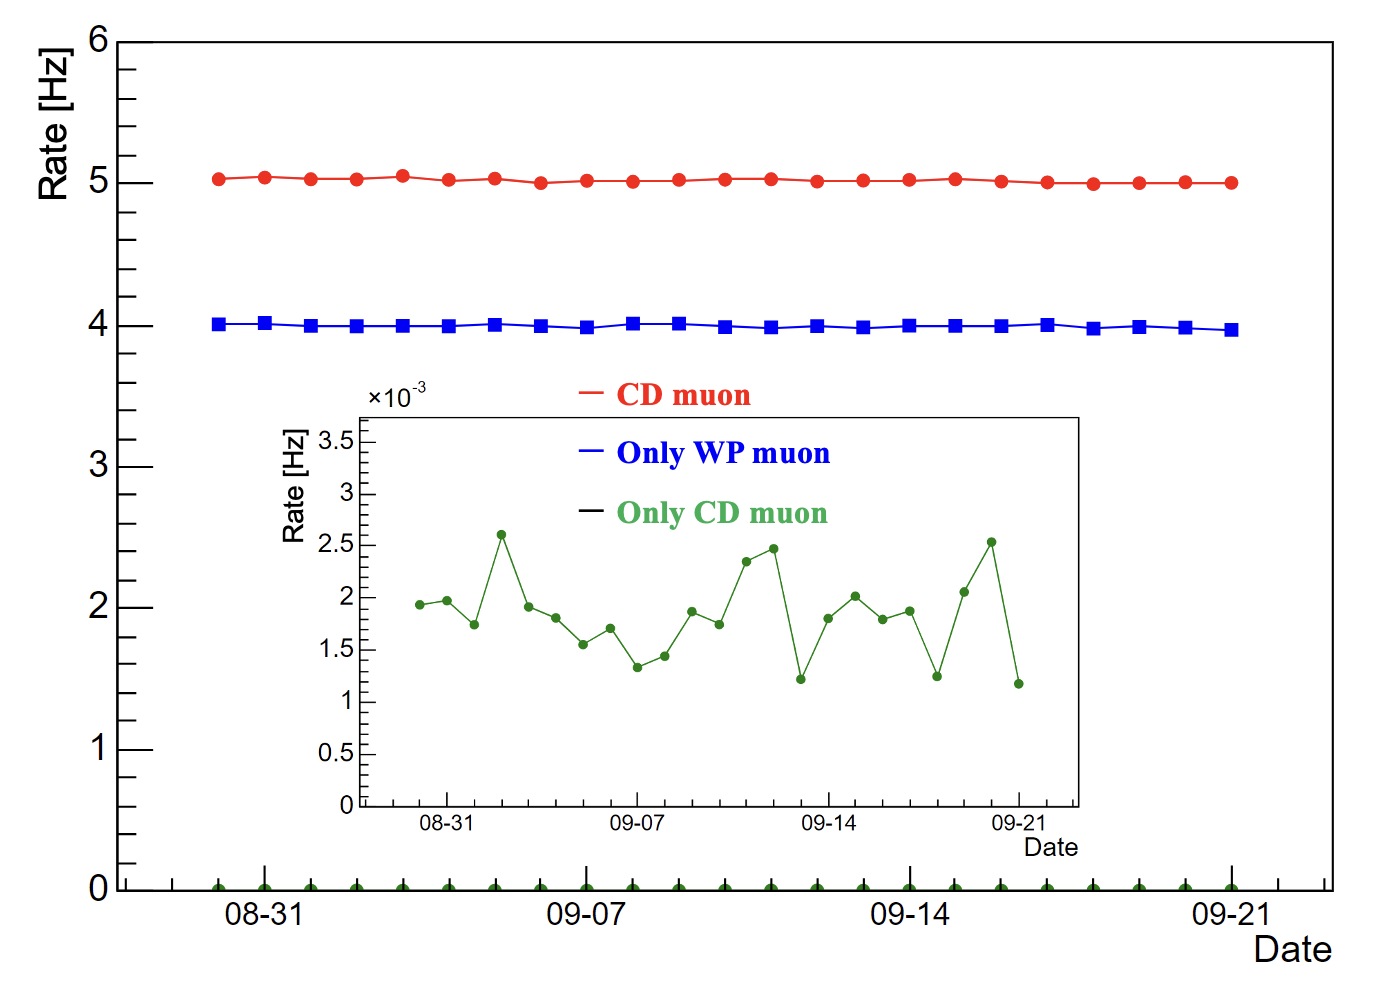
\includegraphics[width=10cm]{2_selection/muon_rate.png}
    \caption{Muon rate as a function of time.}
    \label{fig:muon_rate}
\end{figure}

\subsection{Summary}


Table~\ref{tab:ibd_selection} shows the summary of IBD selection criteria from two groups.
\begin{table}[!htbp]
    \caption{Summary of IBD selection criteria.}
    \label{tab:IbdSel}
    \centering
    \footnotesize% fontsize
    \setlength{\tabcolsep}{4pt}% column separation
    \renewcommand{\arraystretch}{1.2}%row space 
    %\resizebox{\linewidth}{!}{
    \begin{tabular}{lm{6cm}m{6cm}}
        \hline
        Criterion & Selection A1 (IHEP) & Selection A2 (SYSU) \\ 
        \hline
        PMT flasher & Applied & - \\
        %Fiducial volume & \multicolumn{2}{c}{r < 16.5 m, |z| < 15 m} \\
        Fiducial volume & r < 16.5 m, |z|<15.5m & r < 16.9 m, |z|<15.5m \\
        Prompt energy  & (0.7, 12) MeV & [0.7, 12] MeV \\
        Delayed energy & (2.0, 2.5) MeV & [2.0, 2.5] MeV\\
        Coincidence time & (5, 1000) $\mu$s & [5, 1000] $\mu$s \\
        Relative distance & < 1.5 m & < 1.5 m \\
        Multiplicity cut & No other events > 0.7~MeV in the FV or (2.0, 2.5)~MeV outside the FV within 2 ms before  and 1 ms after the delayed & No other events with energy (0.7, 15) MeV in the FV within 2 ms before the delay or within 1 ms after delay \\
        Water pool muon veto & Veto if the delayed is within (0, 5 ms) after NPE > 700 in WP & Veto [-2 $\mu$s, 2 ms] after NPE > 700 in WP \\
        CD muon veto & Veto if the delayed is within (0, 5 ms) after NPE > $3 \times 10^{4}$ in CD & Veto [-1 ms, 6.0 ms] after NPE > $3 \times 10^{4}$ in CD \\
        Spallation neutron veto & Veto if the delayed satisfies $\Delta r$ < 4 m and $\Delta t$ < 1.2 s after spallation neutrons with NPE$_{spn} \in$ (3000, 30000) and $T_{spn2\mu} \in$ (20, 2000) $\mu$s & Veto $\Delta r$ < 4 m and $\Delta t$ < 1.2 s after spallation neutrons  with $E_{spn} \in$ (1.8, 10) MeV and $T_{spn2\mu} \in$ (50, 1000) $\mu$s \\
        \hline
    \end{tabular}
    %}
    \label{tab:ibd_selection}
\end{table}

Figures~\ref{fig:IBD_energy_spectra}, \ref{fig:IBD_energy_spectra_2D}, \ref{fig:IBD_dt}, \ref{fig:IBD_r3} and \ref{fig:IBD_vertex} show the distributions of the selected IBD candidates. Figure~\ref{fig:IBDrate} shows the raw IBD rate as a function of time.

\begin{figure}[!htbp]
    \centering
      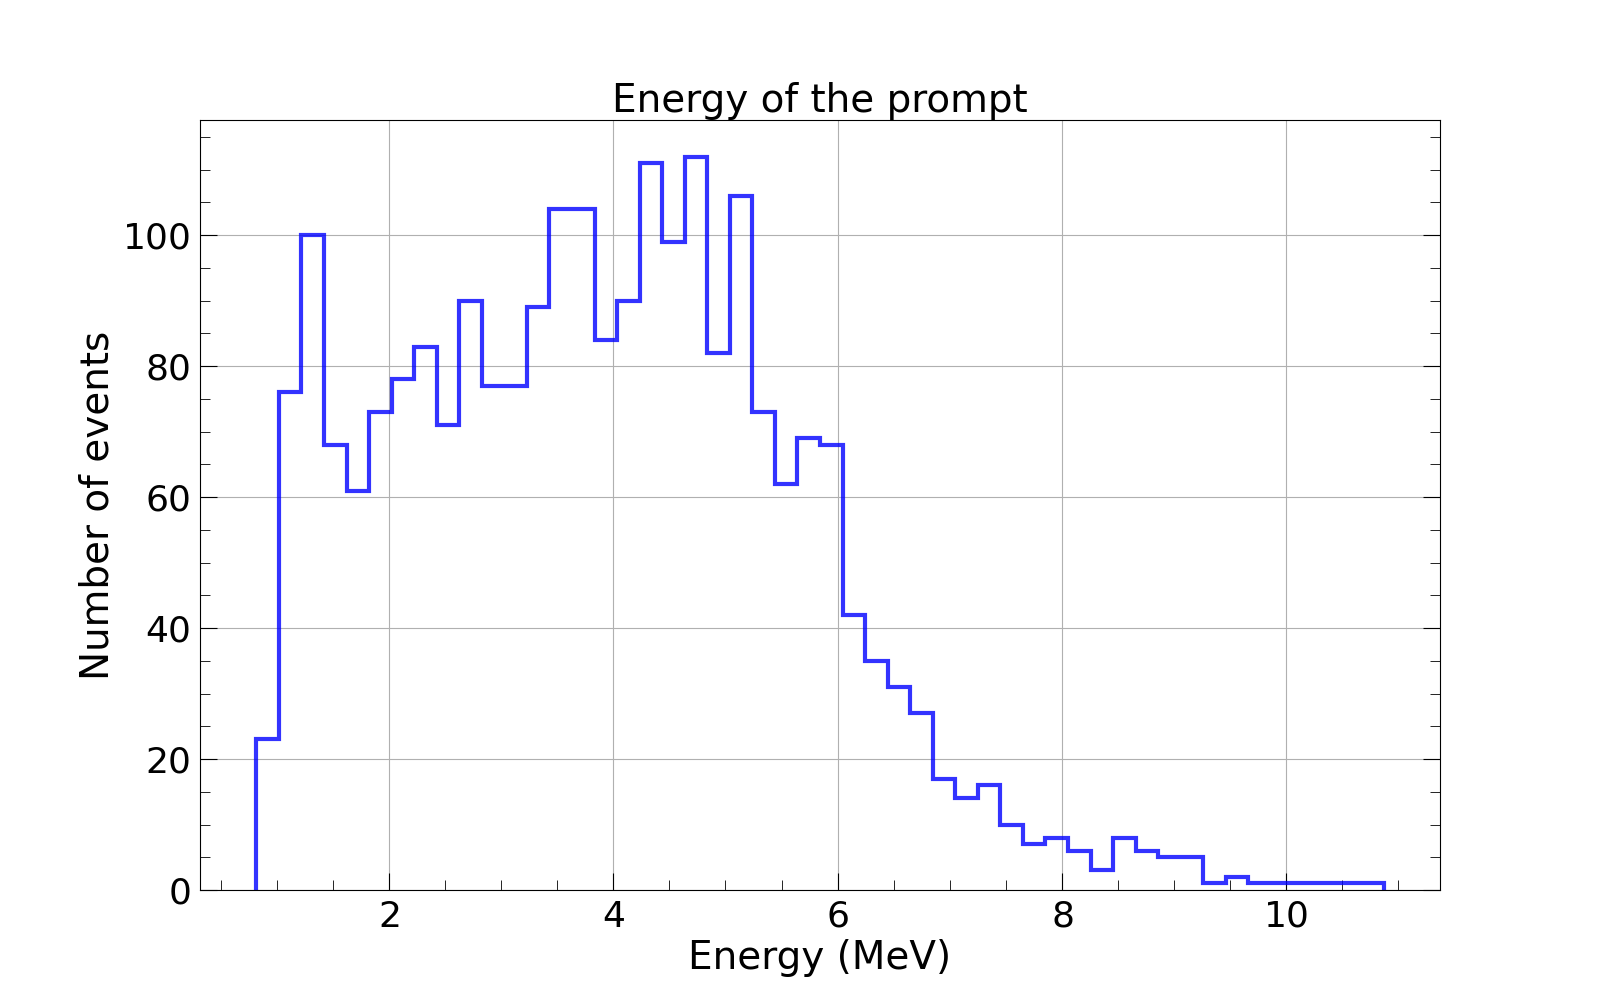
\includegraphics[width=0.49\textwidth]{2_selection/h_ibd_e_p.png}
      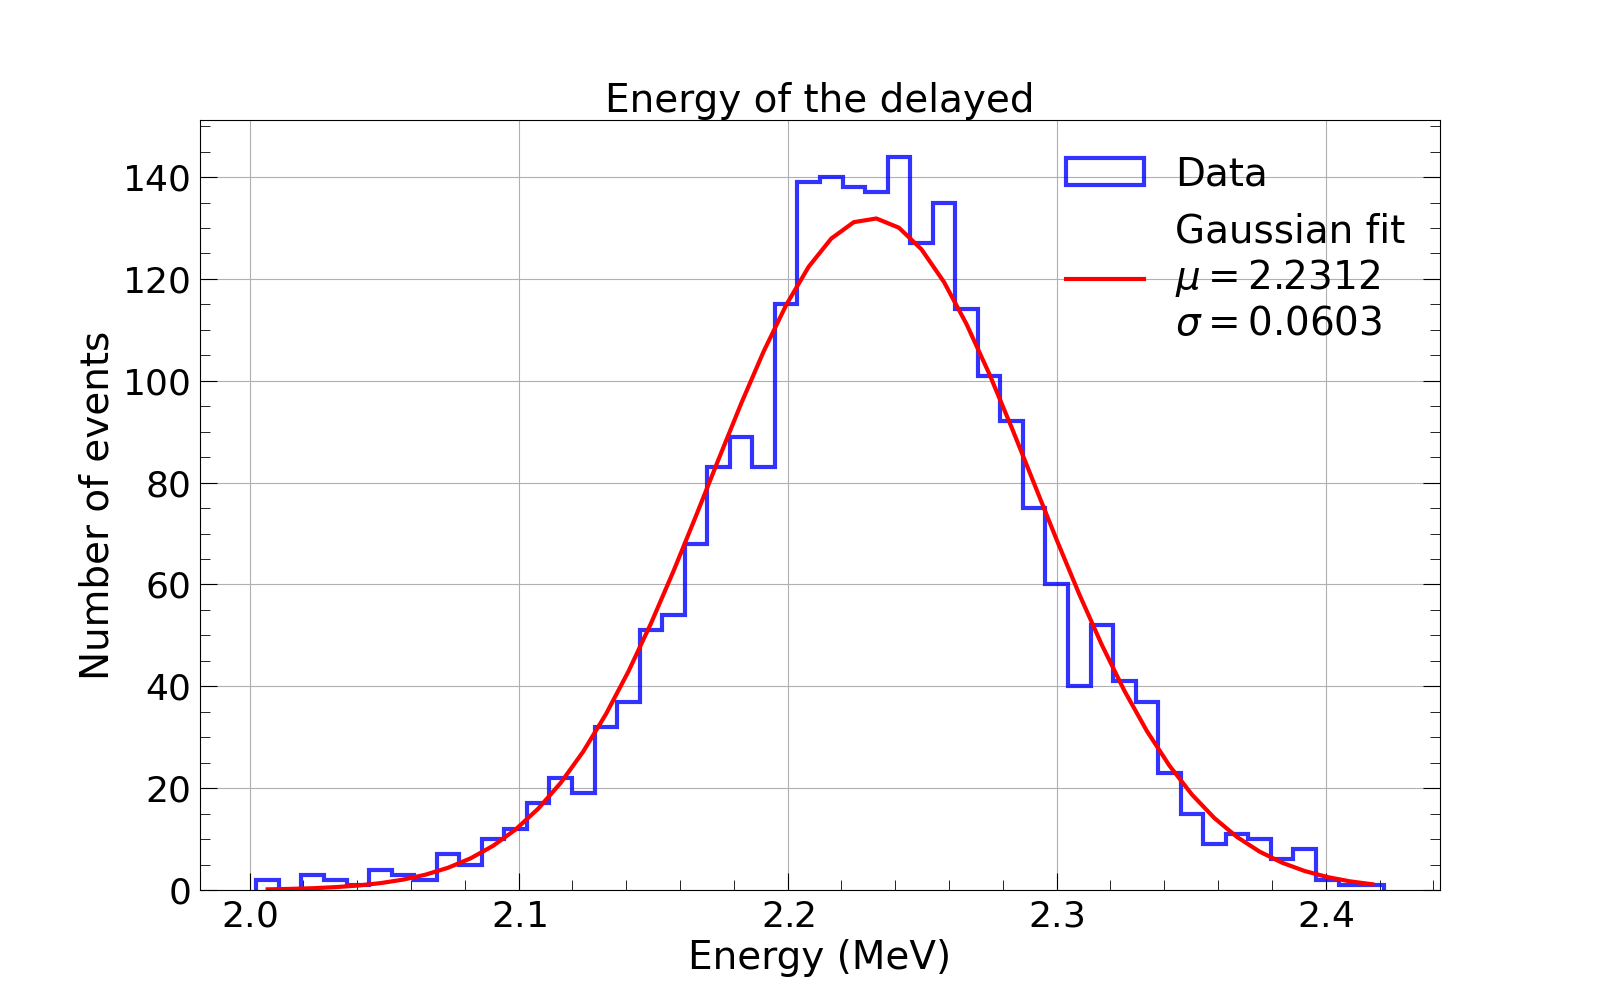
\includegraphics[width=0.49\textwidth]{2_selection/h_ibd_e_d.png}
    \caption{The prompt and delayed energy spectra.}
    \label{fig:IBD_energy_spectra}
\end{figure}


\begin{figure}[!htbp]
    \centering
      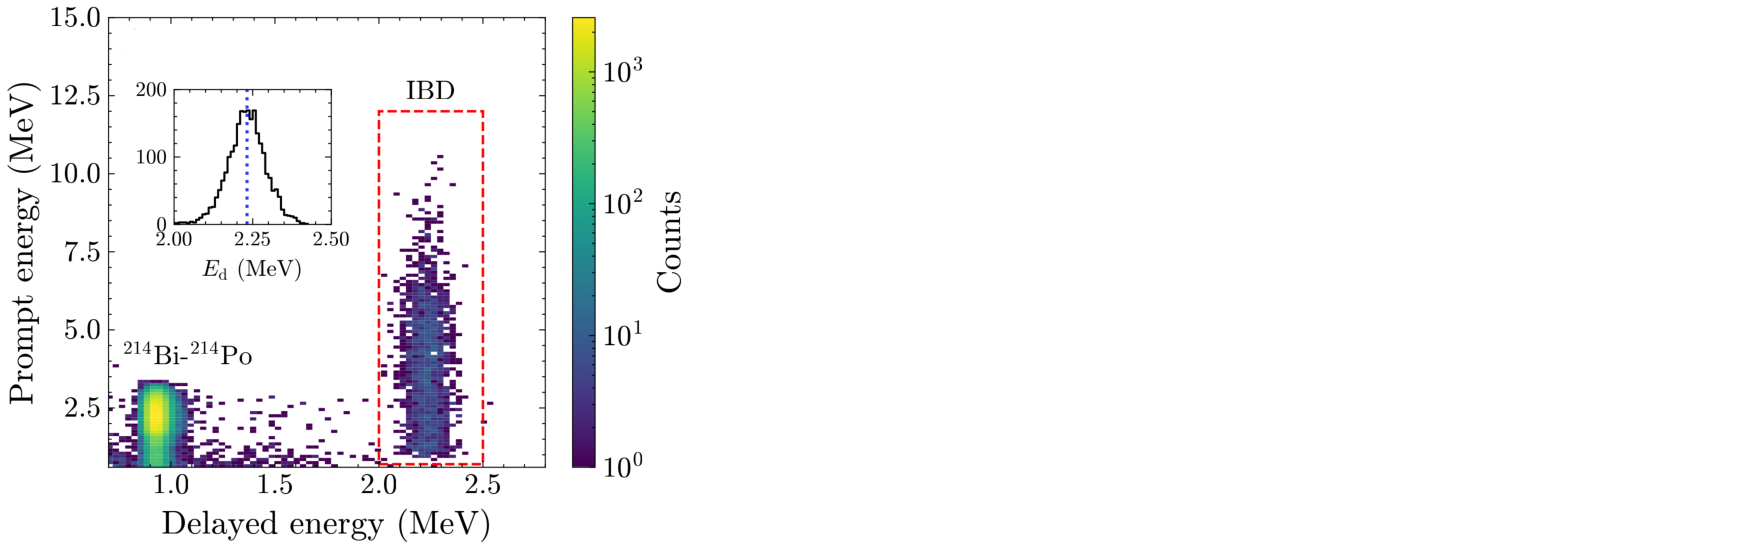
\includegraphics[width=0.7\textwidth]{2_selection/Fig_2D_dt_distance_withgroupABC_noa.pdf}
    \caption{Two-dimensional prompt-versus-delayed energies (with enlarged delayed energy window) showing the $^{214}$Bi-$^{214}$Po cluster at $E_d\sim$1~MeV and the IBD selection region (dashed box).}
    \label{fig:IBD_energy_spectra_2D}
\end{figure}

\begin{figure}[!htbp]
    \centering
    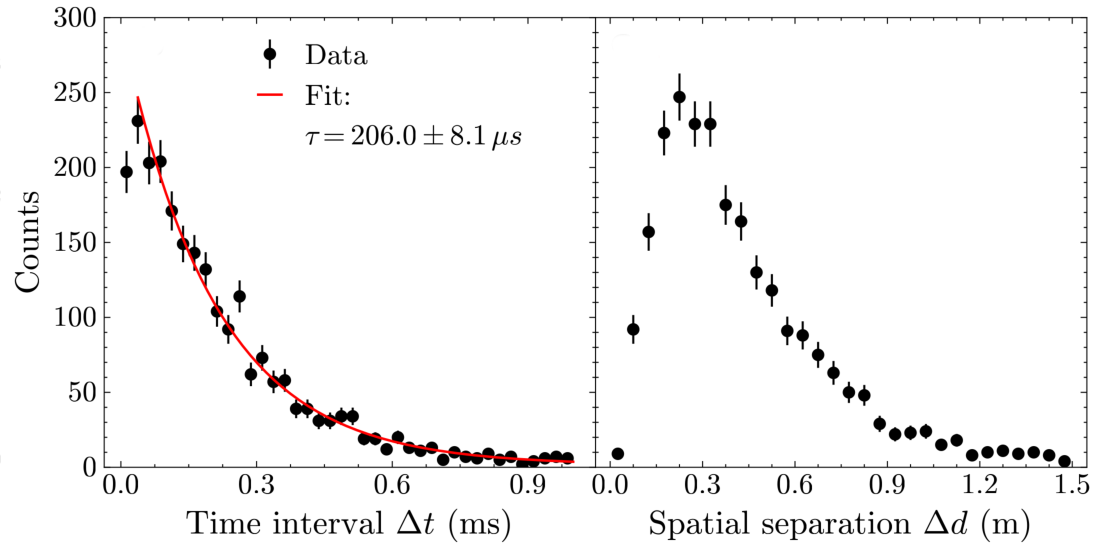
\includegraphics[width=0.8\textwidth]{2_selection/Fig_2D_dt_distance_A.pdf}
    \caption{Left panel: Temporal correlation following an exponential decay with a fitted neutron-capture time of $\tau=206.1\pm8.1\mu s$. The deviation of the first point is due to the $\Delta t >5$~$\mu s$ cut and is therefore not included in the fit. Right panel: Spatial separation $\Delta d$ of the prompt and delayed vertices.}
    \label{fig:IBD_dt}
\end{figure}

\begin{figure}[!htbp]
    \centering
    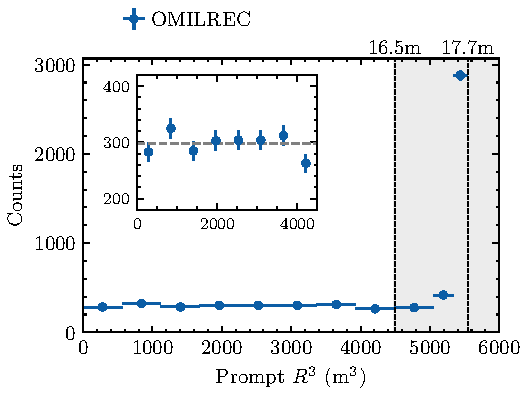
\includegraphics[width=0.8\textwidth]{2_selection/Fig_r3_p_GroupA.pdf}
    \caption{Spatial distribution of reactor neutrino candidates. Prompt-event counts versus reconstructed cubic radius (R3) are shown for the OMILREC. Horizontal bars indicate $R^3$ bin widths; vertical dashed lines mark the FV boundary (16.5 m) and detector edge (17.7 m). The inset shows the uniform event density within the FV, with the dashed line indicating the mean count level. The rising counts beyond the FV are primarily due to accidental coincidences, with minor contributions from fast- and double-neutron backgrounds. }
    \label{fig:IBD_r3}
\end{figure}

\begin{figure}[!htbp]
    \centering
    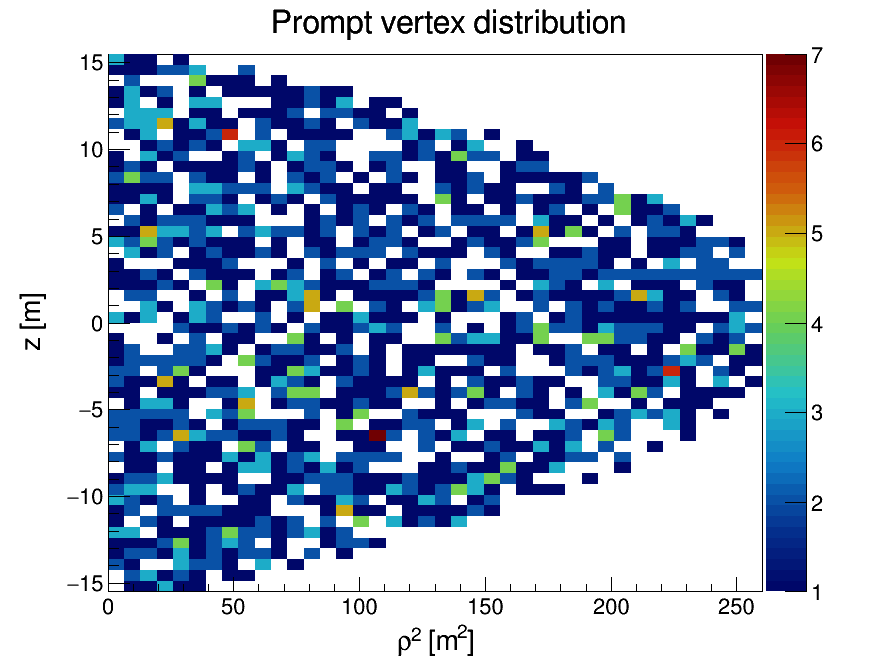
\includegraphics[width=0.49\textwidth]{2_selection/h_ibd_rho_z_p.png}
    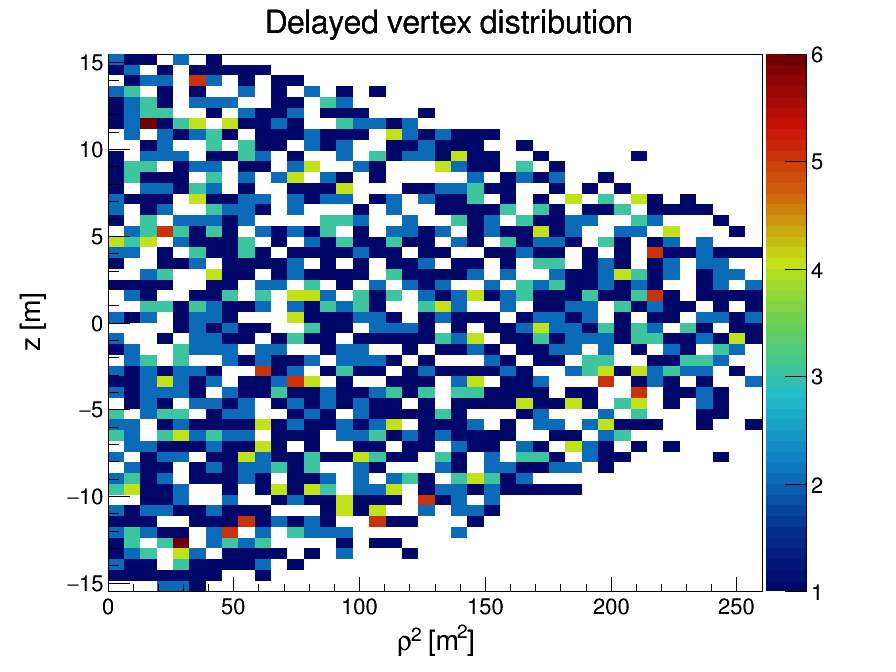
\includegraphics[width=0.49\textwidth]{2_selection/h_ibd_rho_z_d.png}
    \caption{Vertex distribution of the prompt and delayed signals.}
    \label{fig:IBD_vertex}
\end{figure}

\begin{figure}[!htbp]
    \centering
    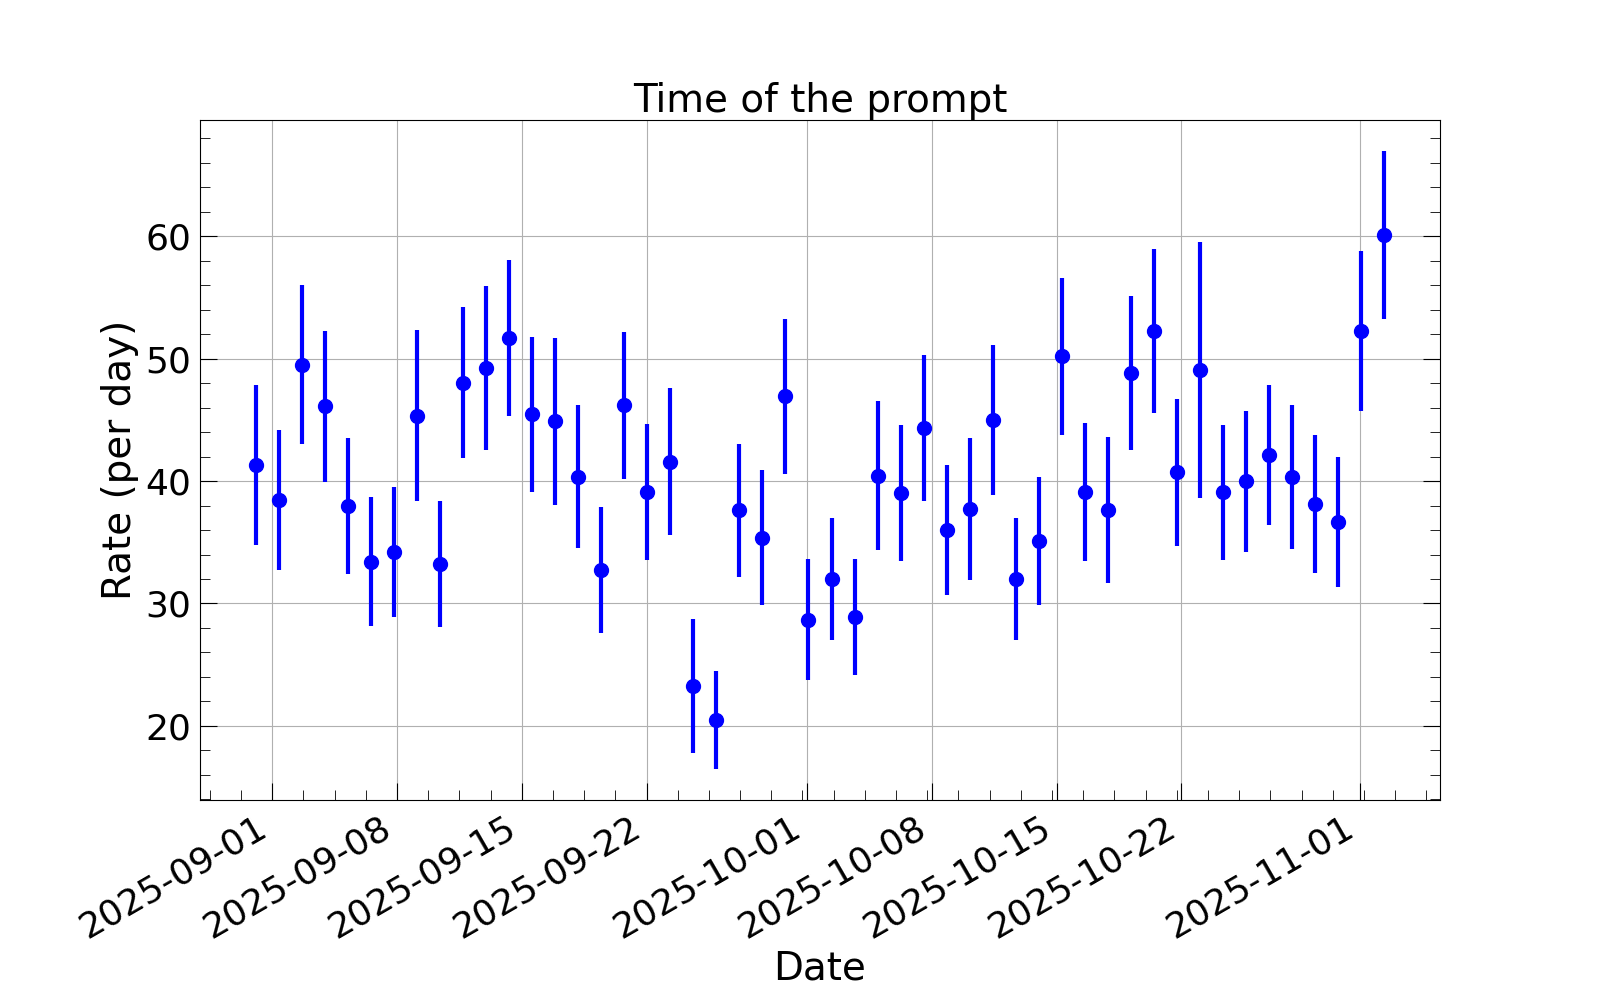
\includegraphics[width=12cm]{2_selection/IBD_rate_reprodb.png}
    \caption{Measured IBD rate as a function of time (no efficiency correction; no background-subtraction).}
    \label{fig:IBDrate}
\end{figure}

%\begin{figure}[!htbp]
%    \centering
%    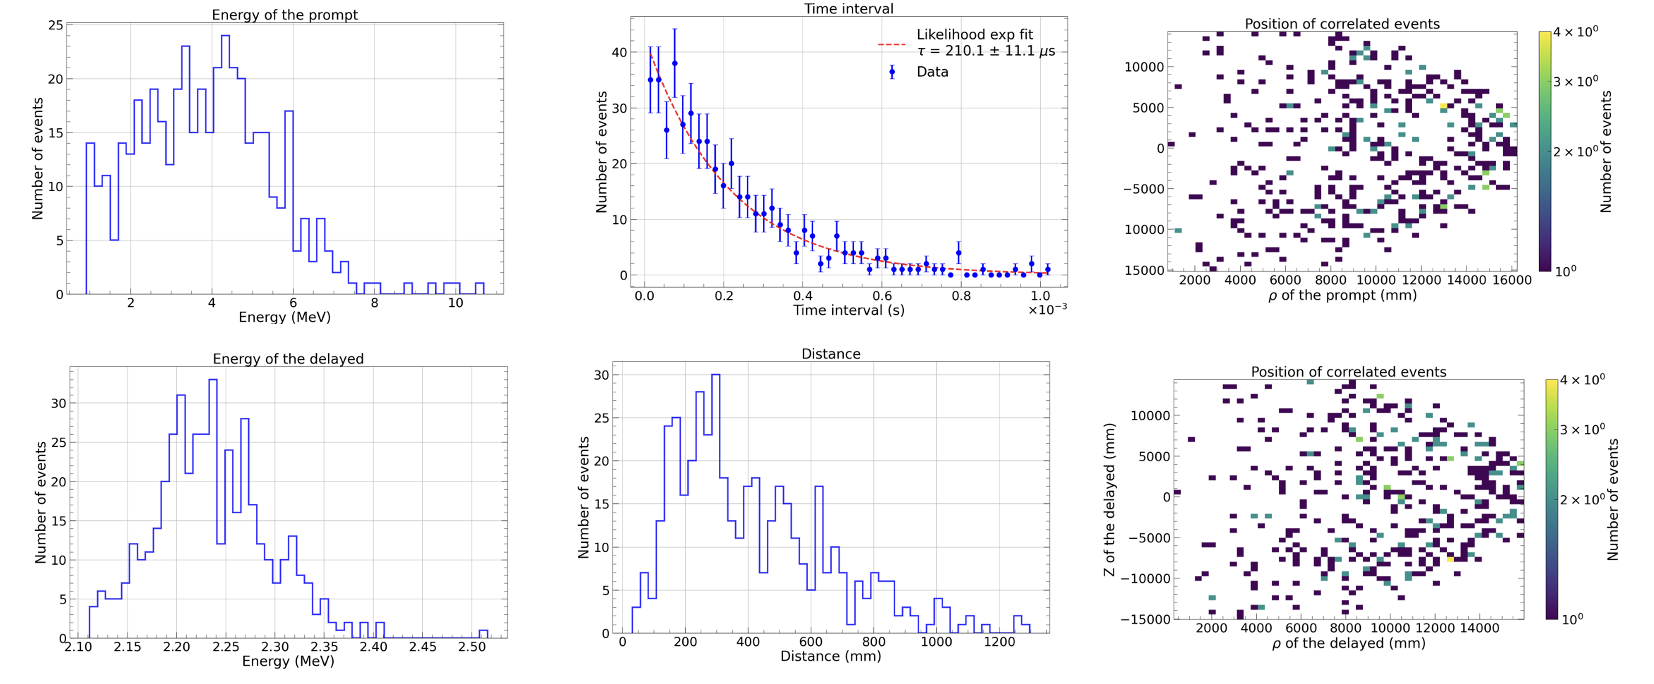
\includegraphics[width=0.9\textwidth]{2_selection/IBD_ReProdA25.png}
%    \caption{IBD distributions using ReProd25A.}
%    \label{fig:IBD_vertex}
%\end{figure}

\section{Background analysis}
\label{sec:background}

\subsection{Flashers}
Flashing PMT induced backgrounds, i.e., flashers were discriminated by the fired PMT T/Q pair information. Here the standard deviations of fired PMTs' T/Q pair number and T/Q pairs' hit time were used:
$\sigma_{N_{\text{hit}}} = \sqrt{ \frac{1}{m-1} \sum_{i=1}^{m} \left( N_{\text{hit},i} - \bar{N}_{\text{hit}} \right)^2 }$, where $\bar{N}_{\text{hit}} = \frac{1}{m} \sum_{i=1}^{m} N_{\text{hit},i}$, $m$ is the fired PMT number; and $\sigma_{t_{\text{hit}}} = \sqrt{ \frac{1}{n-1} \sum_{j=1}^{n} \left( t_{\text{hit},j} - \bar{t}_{\text{hit}} \right)^2 }$, where $\bar{t}_{\text{hit}} = \frac{1}{n} \sum_{j=1}^{n} t_{\text{hit},j}$, $n$ is the hit number. Based on the 2D distribution of the two variables shown in fig \ref{fig:flasherdistribution}, we developed an ellipse cut as defined:
\begin{equation}
    \epsilon=\left( \frac{\sigma_{N_{\text{hit}}} - 0.55}{0.45} \right)^2
+ \left( \frac{\sigma_{t_{\text{hit}}} - 170}{80} \right)^2 < 1
\end{equation}

\begin{figure}
    \centering
    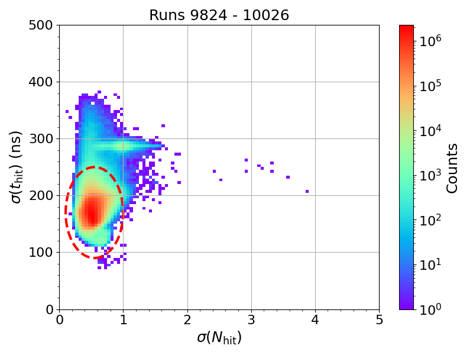
\includegraphics[width=0.5\linewidth]{3_background/fig_flasher_discriminate_quantities.png}
    \caption{2D distribution of $\sigma_{t_{\text{hit}}}$ v.s. $\sigma_{N_{\text{hit}}}$. Select CD triggers with $E_\text{rec}\in(0.7, 12]~\mathrm{MeV}$ after cosmic-ray muon veto from physics runs. The ellipse cut region is marked with the red dashed line.}
    \label{fig:flasherdistribution}
\end{figure}

Beyond the ellipse cut region, the CD triggers are considered "nonphysical", which are mainly contributed by the flashers. About 0.05 Hz events are cut off in normal runs. By assuming that all cut off events are physical triggers, we can estimate that the upper limit on the inefficiency is less than 0.1\% (shown in fig \ref{fig:flasherinefficiency}). Runs with a rate higher than this are classified as 'abnormal' due to their flasher-rich nature. Unlike normal runs, abnormal runs show a distinct peak caused by flashers. As shown in fig \ref{fig:flashercontamination}, the separation between physical events and flashers becomes clearer as the energy increases. There may be a inflection point between the peaks formed by physical events and flashers. The contamination from remaining flashers, estimated by extending the inflection point into the signal region, does not exceed 0.05\% in the worst case.

\begin{figure}[htbp]
    \centering
    \begin{subfigure}[b]{0.19\textwidth}
        \centering
        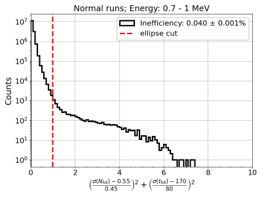
\includegraphics[width=\textwidth]{3_background/fig_flasher_inefficiency_0.7-1.png}
    \end{subfigure}
    \begin{subfigure}[b]{0.19\textwidth}
        \centering
        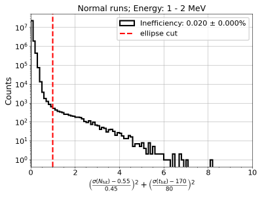
\includegraphics[width=\textwidth]{3_background/fig_flasher_inefficiency_1-2.png}
    \end{subfigure}
    \begin{subfigure}[b]{0.19\textwidth}
        \centering
        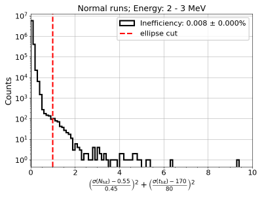
\includegraphics[width=\textwidth]{3_background/fig_flasher_inefficiency_2-3.png}
    \end{subfigure}
    \begin{subfigure}[b]{0.19\textwidth}
        \centering
        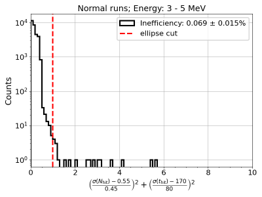
\includegraphics[width=\textwidth]{3_background/fig_flasher_inefficiency_3-5.png}
    \end{subfigure}
    \begin{subfigure}[b]{0.19\textwidth}
        \centering
        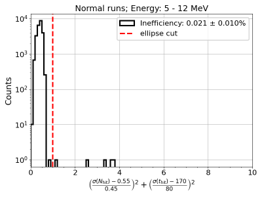
\includegraphics[width=\textwidth]{3_background/fig_flasher_inefficiency_5-12.png}
    \end{subfigure}
    \caption{CD physical triggers inefficiency of flasher cut in different energy ranges. $\epsilon$ distributions of normal runs are used. }
    \label{fig:flasherinefficiency}
\end{figure}

\begin{figure}[htbp]
    \centering
    \begin{subfigure}[b]{0.19\textwidth}
        \centering
        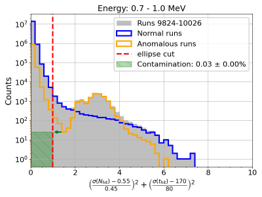
\includegraphics[width=\textwidth]{3_background/fig_flasher_contamination_0.7-1.png}
    \end{subfigure}
    \begin{subfigure}[b]{0.19\textwidth}
        \centering
        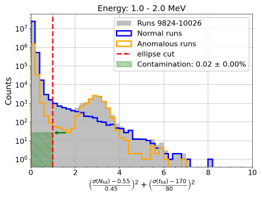
\includegraphics[width=\textwidth]{3_background/fig_flasher_contamination_1-2.png}
    \end{subfigure}
    \begin{subfigure}[b]{0.19\textwidth}
        \centering
        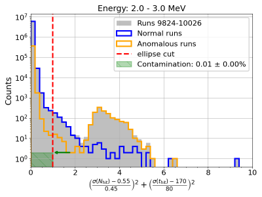
\includegraphics[width=\textwidth]{3_background/fig_flasher_contamination_2-3.png}
    \end{subfigure}
    \begin{subfigure}[b]{0.19\textwidth}
        \centering
        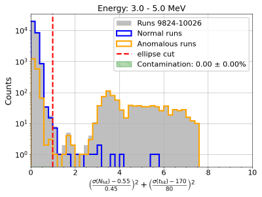
\includegraphics[width=\textwidth]{3_background/fig_flasher_contamination_3-5.png}
    \end{subfigure}
    \begin{subfigure}[b]{0.19\textwidth}
        \centering
        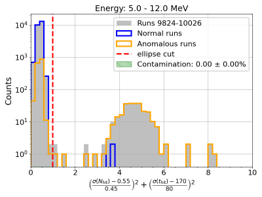
\includegraphics[width=\textwidth]{3_background/fig_flasher_contamination_5-12.png}
    \end{subfigure}
    \caption{Flasher contamination after cut in different energy ranges. Green regions are the extension of inflection point, which can be seen as the remained flashers.}
    \label{fig:flashercontamination}
\end{figure}

%\td{Uncertainty and inefficiency for IBD? Need selected IBD's distribution}

\subsection{Accidental background}
The accidental background was determined using an time-offwindow method. This technique employs selection criteria identical to the standard IBD analysis, except for the coincidence time window applied to the prompt and delayed signals. We pair delayed-like events with prompt-like candidates taken from time windows far away from the true coincidence region. For each delayed candidate that passes the muon and multiplicity vetoes, the algorithm shifts the delayed time backward by 2, 10, 12, 17, and 30 s, forming 500 off-time windows (100 windows for each main time offset). Within each shifted window, a virtual delayed signal is placed at the edge of the window, and we search for prompt-like events that satisfy the same energy, spatial, and time-difference cuts as real IBD pairs. Both the delayed and prompt candidates must also pass their own muon and multiplicity vetoes, ensuring that no muon or nearby activity occurs within the veto windows before or after each candidate. The scheme is shown in Fig.~\ref{fig:off_window}.

\begin{figure}
    \centering
    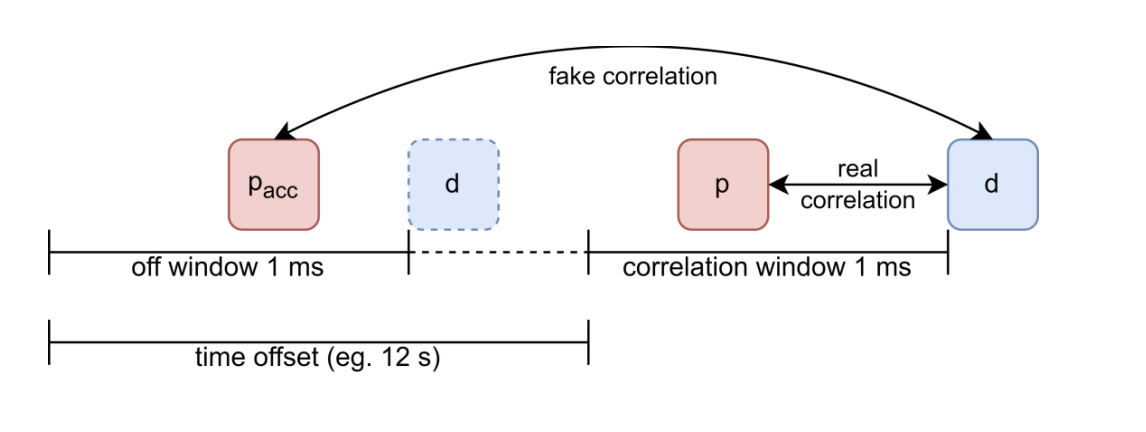
\includegraphics[width=0.8\linewidth]{2_selection/off_window_scheme.png}
    \caption{The scheme of the off-window method. }
    \label{fig:off_window}
\end{figure}

The time-offwindow method requires additional selections and corrections. Although it follows the same selection strategy as the standard IBD selection, the impact of muon-related backgrounds differs. In the standard IBD selection, the prompt signal is close to the delayed signal and thus well separated from muons. But in the time-offwindow method, the prompt signal can be close to muons. We apply an additional muon veto and multiplicity cut on the virtual delayed signal and correct the efficiency, to make sure the results from both selections consistent. This procedure was validated using simulation dataset as shown in Fig.~\ref{fig:off_window_correction}..

\begin{figure}
    \centering
    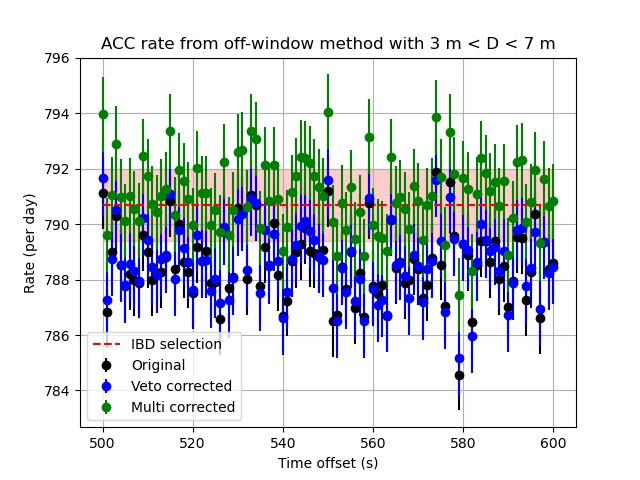
\includegraphics[width=0.7\linewidth]{3_background/rate_off_window_500s_fastn_fv176_eos.png}
    \caption{Validation of the correction on time-offwindow method with released distance cut. The difference is decreased from 0.26\% to 0.04\% after correction.}
    \label{fig:off_window_correction}
\end{figure}

The accidental background was found to be 0.049$\pm$0.003 counts per day for the fiducial volume $r<16.5$~m, |z|<15.5~m. The uncertainty of this measurement is dominated by the statistical uncertainty in the event rate measured within the off-time window. The results are shown in Fig.~\ref{fig:ACC_rate_shape} and Fig.~\ref{fig:ACC_vertex}.

\begin{figure}[!htbp]
    \centering
    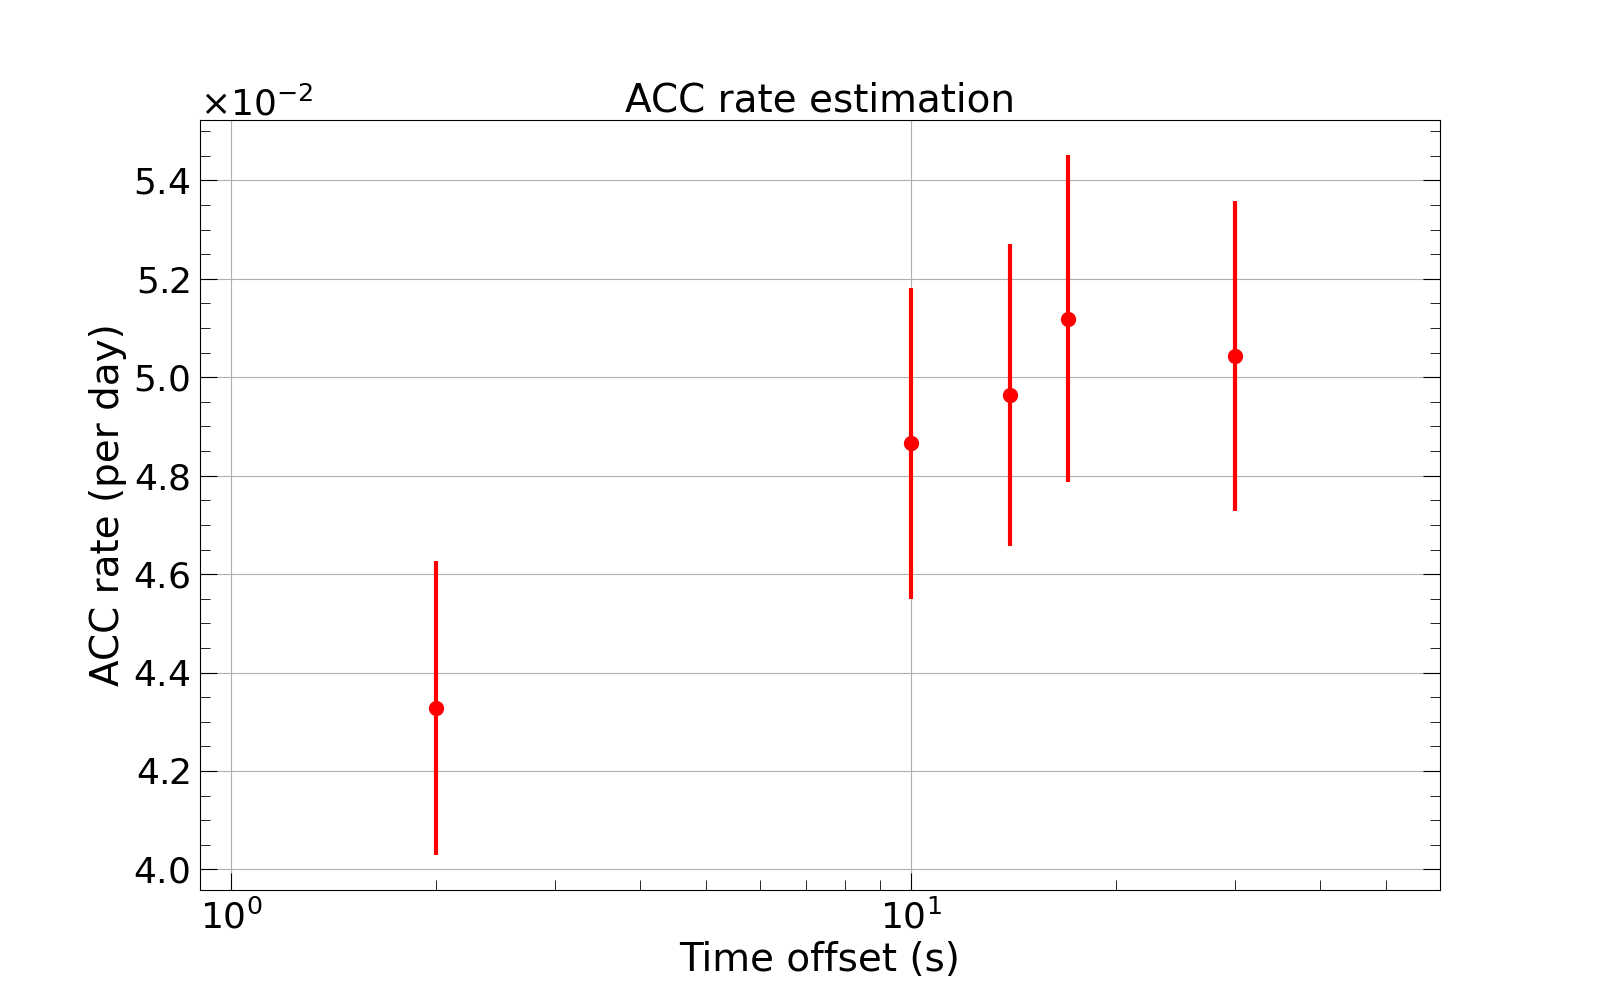
\includegraphics[width=0.49\textwidth]{3_background/h_good_d_15_rate_acc_main_eff.png}
    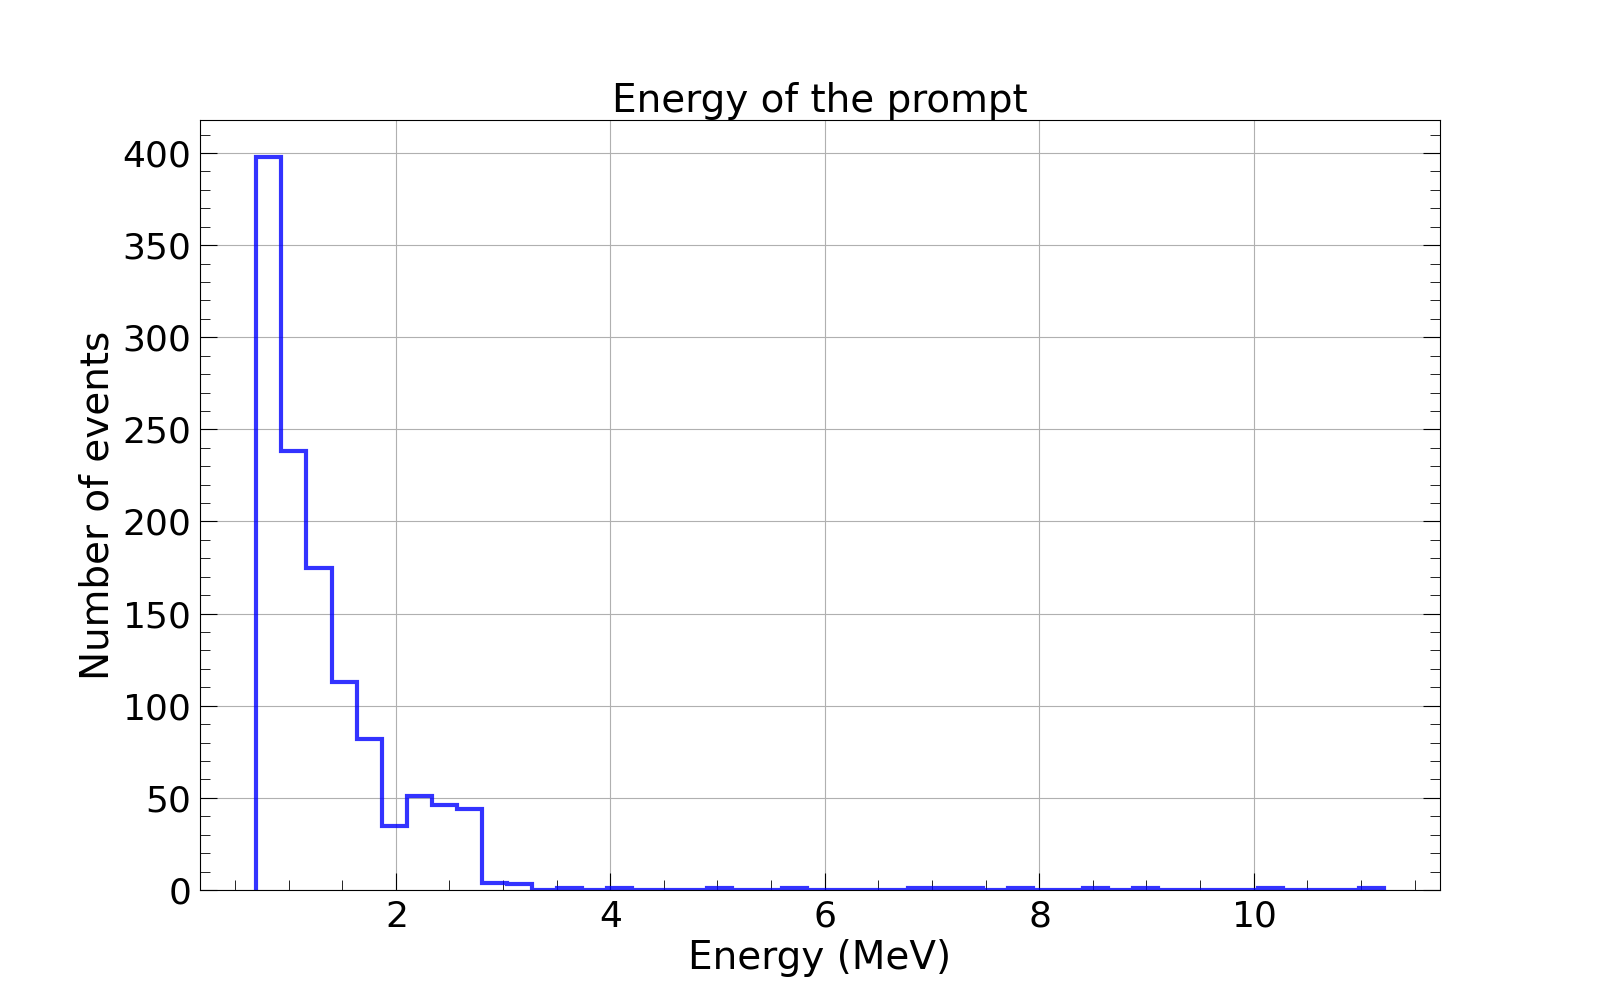
\includegraphics[width=0.49\textwidth]{3_background/h_good_d_15_e_p_0.png}
    \caption{Left: Estimated rate with extra veto and multiplicity cut efficiency correction. Right: Energy spectrum of the prompt signal of accidental coincidence background.}
    \label{fig:ACC_rate_shape}
\end{figure}

\begin{figure}[!htbp]
    \centering
    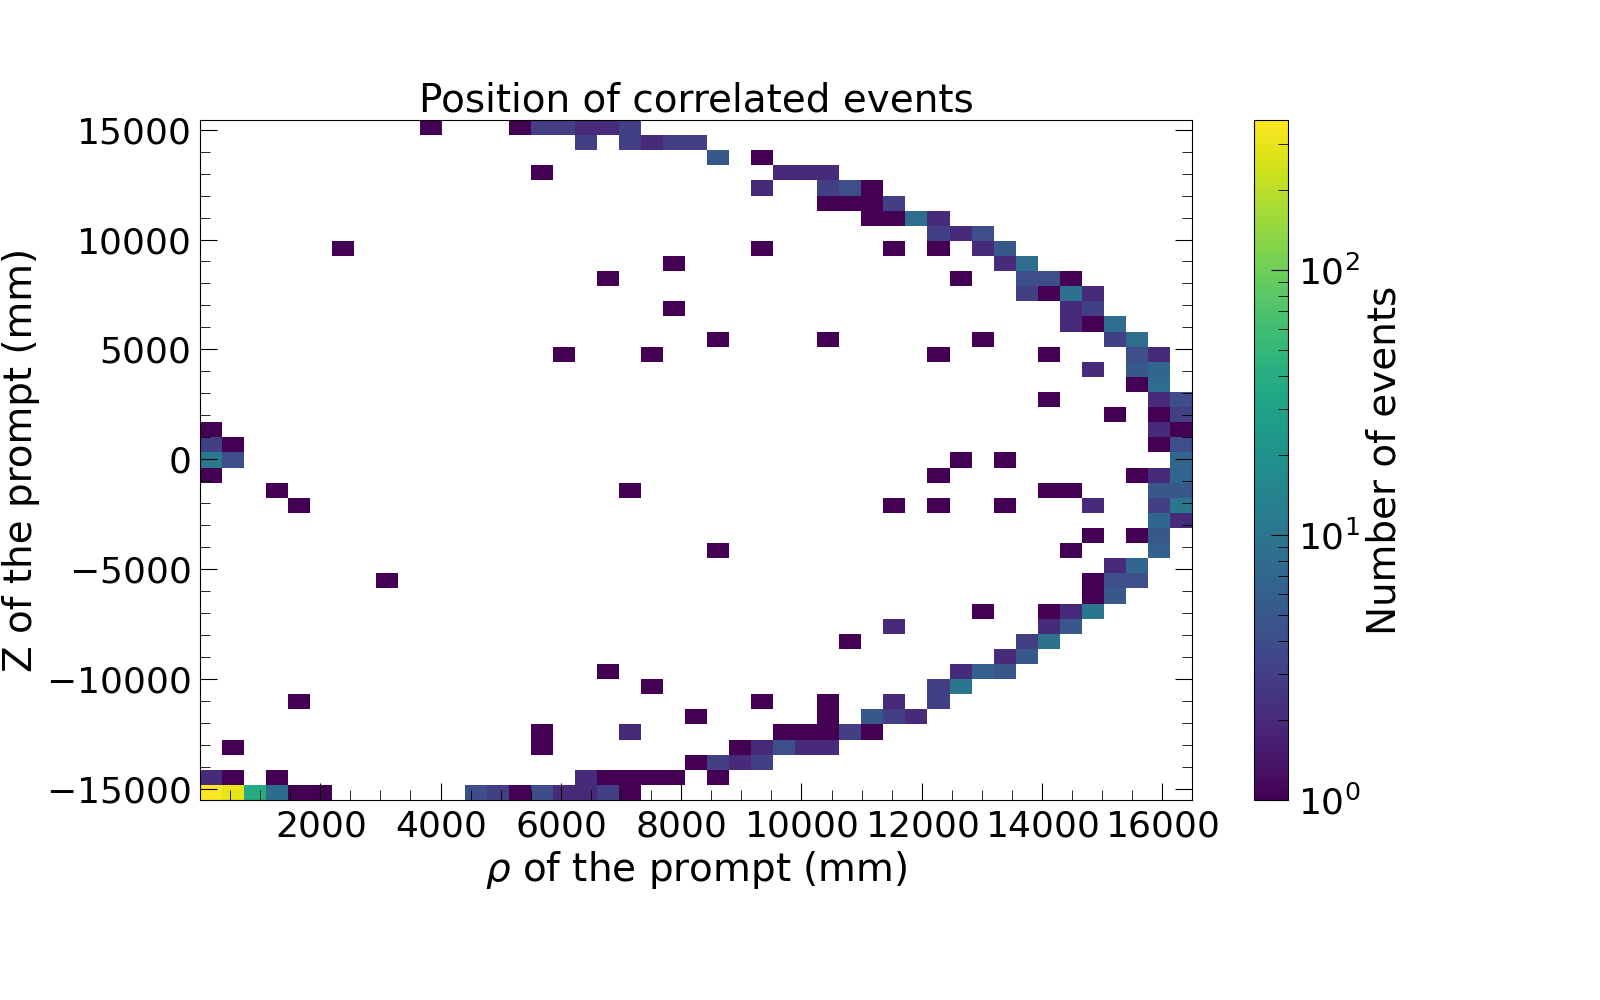
\includegraphics[width=0.49\textwidth]{3_background/h_good_d_15_rho_z_p_0.png}
    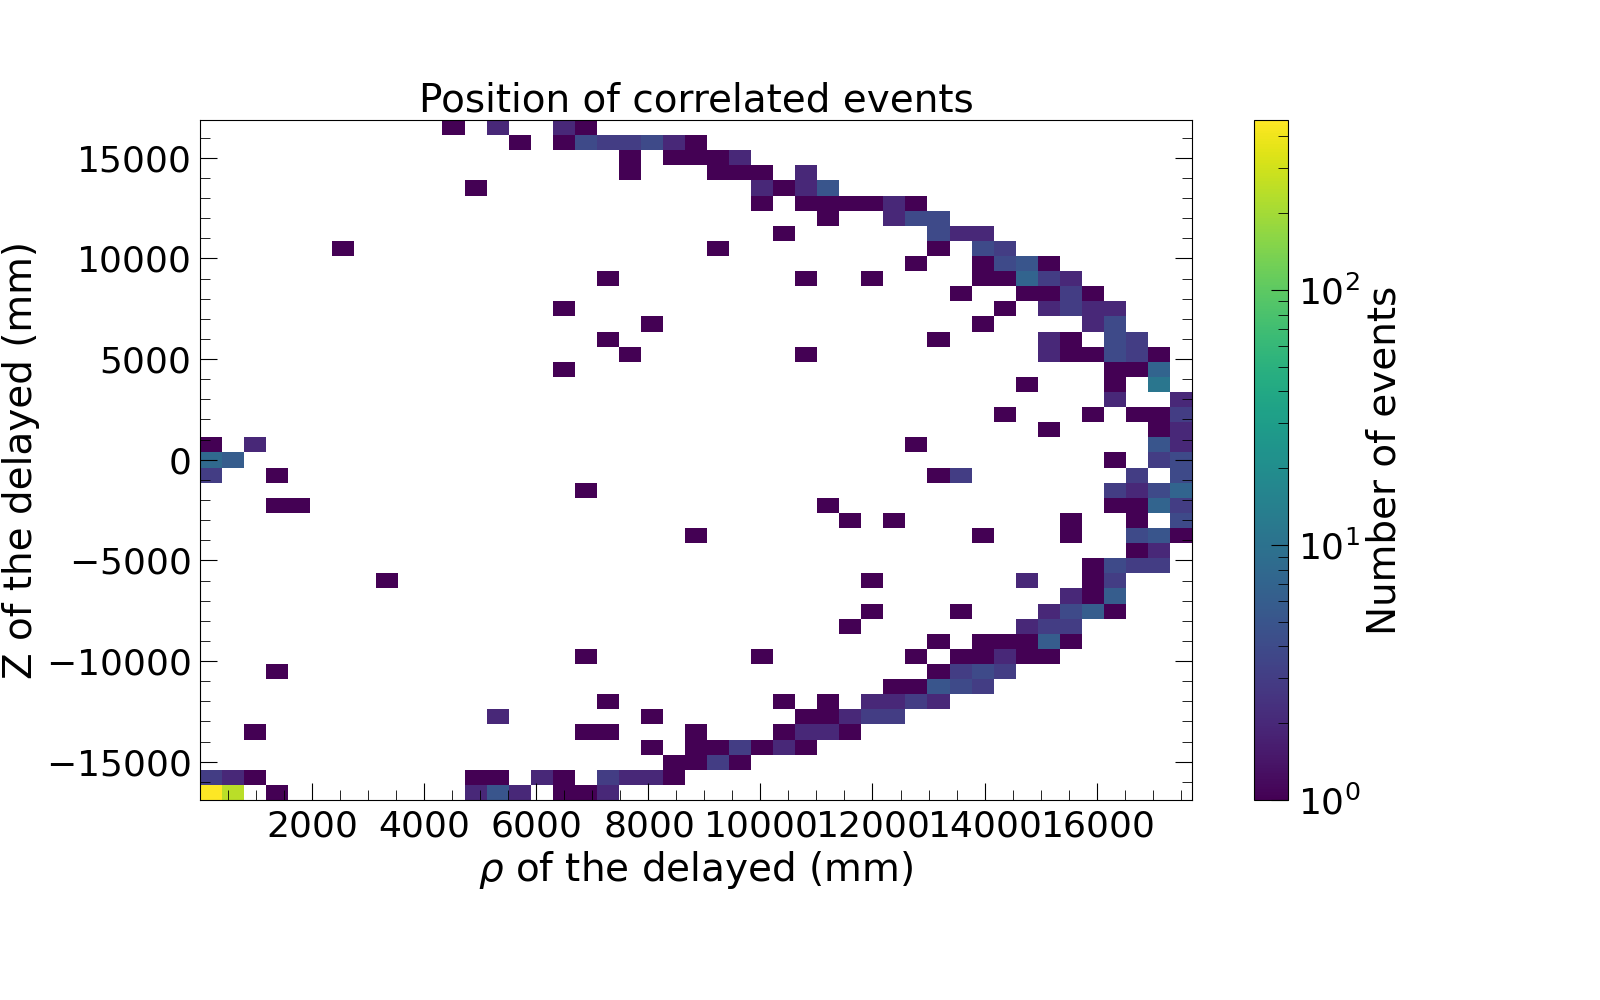
\includegraphics[width=0.49\textwidth]{3_background/h_good_d_15_rho_z_d_0.png}
    \caption{Vertex distribution of the prompt and delayed signals selected by off-window method.}
    \label{fig:ACC_vertex}
\end{figure}

\subsection{\Li}
Cosmogenic induced spallation isotopes on $^{12}$C in the LS can become a correlated background for IBD. Among them, $^9$Li and $^8$He are the dominant ones, each with a branching ratio of 51\% and 16\% $\beta$-neutron cascade decay. The $\beta$ decays have a Q value of 13.6 MeV for $^9$Li and 10.7 MeV for $^8$He. They have a relatively long half-life of 178.0 ms and 119.0 ms, respectively \cite{nndc}. The $^{9}$Li/$^{8}$He yield is derived from a time-since-last-muon fit, as it is produced by muon unlike the IBD. More details on the methods can be found in \cite{li9_doc_db}.

\subsubsection{Yield evaluation}
% \textcolor{red}{numbers are to update with ReprodB}

The dataset used in this results is based on the same one for IBD selection, i.e. ReProd25C with OMIREC reconstruction. An IBD sample is prepared with the same selection criteria as A1, but no spallation neutron veto or any shower muon veto to retain $^{9}$Li/$^{8}$He in the sample. The muon is defined as a CD trigger (Q>3e4 PE) with a correlated WP trigger (Q>1e3 PE) within $\pm$5$\mu$s. The time since last muon distribution is fitted by the following function:

\begin{equation}
    N(t) = \sum_{iso}N_{iso}\lambda_{iso}e^{-\lambda_{iso}t} + N_\mathrm{(IBD+Acc+iso2)}R_\mu e^{-R_\mu t}
\end{equation}

where $iso$ runs over $^9$Li, $^8$He, $\lambda_{iso}=R_\mu+1/\tau_{iso}$, and $R_\mu$ is the muon rate. $N_\mathrm{IBD+Acc+iso2}$ represents IBD events, Accidental events and $^{9}$Li/$^{8}$He uncorrelated to the muon. The fraction between the number of $^8$He and $^9$Li events is fixed to be 0.0143. The time since the last muon fit does not work when the muon rate is high. In Figure~\ref{fig:time_fit_li9}, example fits are shown for the time since the last muon of different visible energies. The fitted muon rates are consistent with the rates calculated by counting. $^{9}$Li/$^{8}$He events are produced by muons with high-energy deposits during showers. Clear $^{9}$Li/$^{8}$He are fitted for muon energy larger than 1e7 pe ($\sim$5 GeV). For muon energy smaller than 1e7 PE, the fit gives a much smaller number of $^{9}$Li/$^{8}$He, the error is very large due to a much worse $^{9}$Li/$^{8}$He to IBD ratio. We also tried to float the lifetime of $^{9}$Li/$^{8}$He, and the fitted lifetime is consistent with $^{9}$Li/$^{8}$He lifetime within uncertainties.

To properly take into account the correlations between the four time-since-last-muon distributions in different muon energy slices, a joint fit of the four energy slices is performed. The fitted error is also cross checked with another MC and  bootstrap methods. And they are found consistent. 

\begin{figure}
    \centering
    \includegraphics[width=0.8\linewidth]{3_background/time_fit_li9_example.png}
    \caption{Time since last muon fit for different muon visible energy (PE) regions: [1e6, 7e6], [7e6, 1e7], [1e7, 1.2e7], [1.2e7, 2e9] (from left to right, top to down). }
    \label{fig:time_fit_li9}
\end{figure}

To increase the $^{9}$Li/$^{8}$He event purity in the IBD sample, we require events with $E_p>6$ MeV. The results is summarized in Figure~\ref{fig:fitted_rate_comp}. The fraction of events with with $E_p>6$ MeV over $E_p>0.7$ MeV 0.40$\pm$0.06, compared to the predictions of 0.40/0.36 from DYB/common input. Note that the results for $E_{p}$ $>$ 0.7 MeV in Figure~\ref{fig:fitted_rate_comp} are derived from direct fitting.

For $^{9}$Li/$^{8}$He events generated by $Q_\mu$<5e6 PE, we use the correction factor from MC truth \cite{li9_doc_db}. After taking into account the selection efficiency ($\sim$0.6988) as well \cite{li9_doc_db}, the $^{9}$Li/$^{8}$He yield ($\beta$-$n$ branch) is evaluated to be 73.6$\pm$2.7 cpd. This yield is derived from the total fitted SPN-tagged events plus the residual events following SPN veto.

\begin{figure}
    \centering
    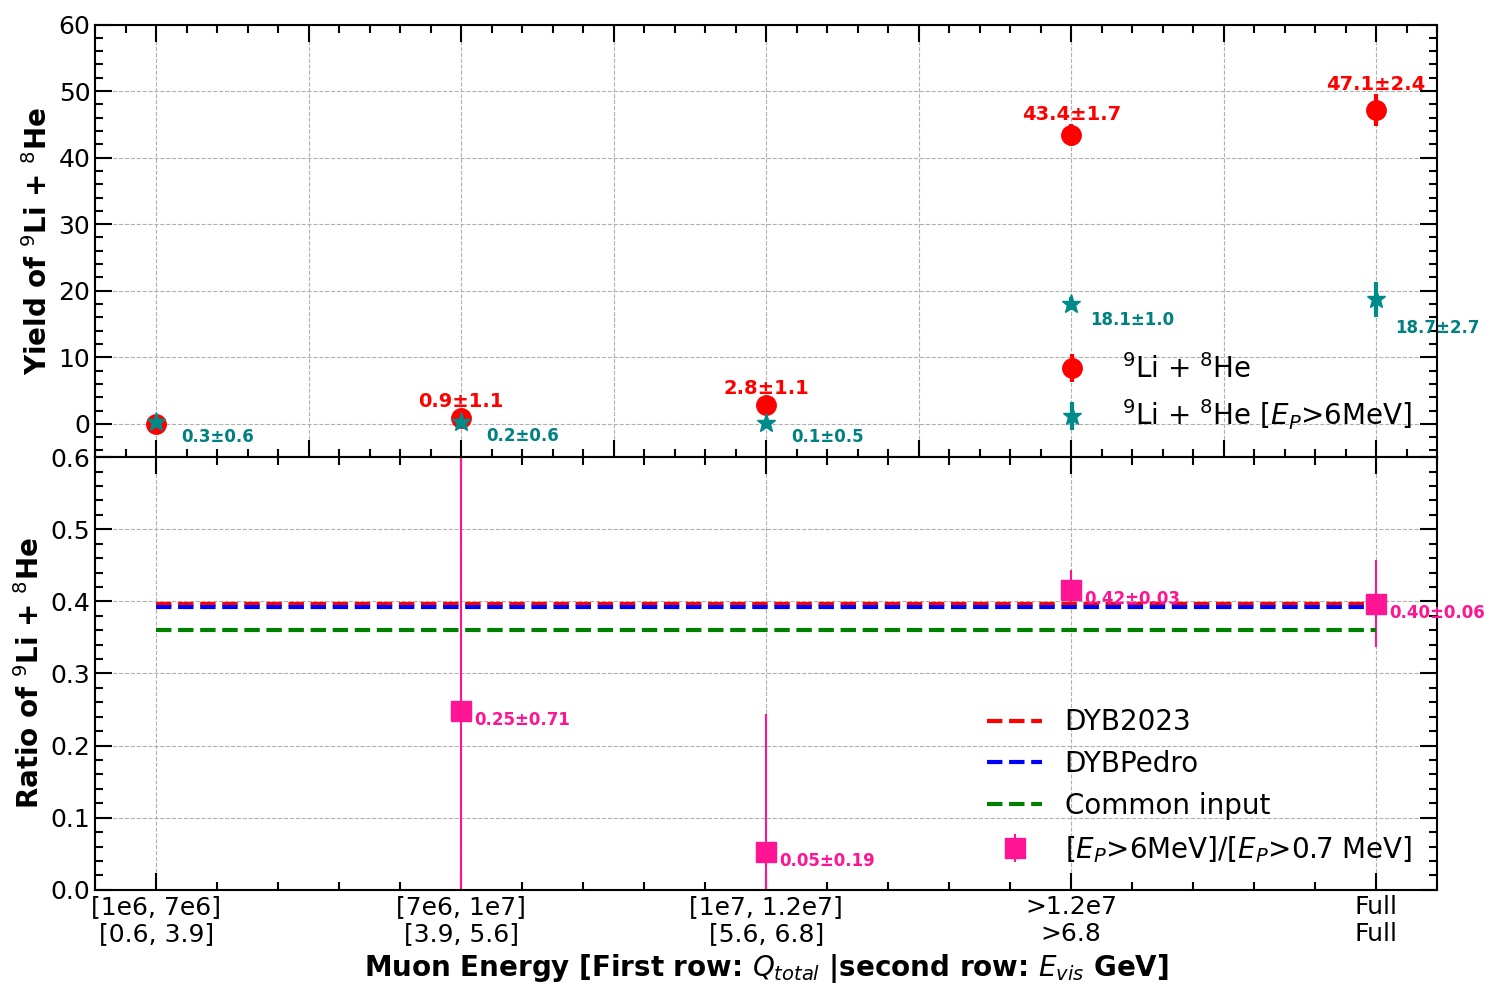
\includegraphics[width=0.7\linewidth]{3_background/fitted_rate_comp_w_Ep_gt_6MeVnew.png}
    \caption{Fitted $^{9}$Li/$^{8}$He rate comparison with a prompt energy cut of $>$6 MeV.}
    \label{fig:fitted_rate_comp}
\end{figure}

% \begin{table}[!htbp]
%     \caption{\Li rate summary.}
%     \label{tab:li9}
%     \centering
%     \begin{tabular}{c|cccc}
%         \hline
%         Muon energy [PE] & $<$5e6 & [5e6, 1e7] & [1e7, 2e7] & $>$2e7 \\
%         \hline
%         Livetime [day] & \multicolumn{4}{c}{33.1} \\
%         \hline
%         Counts      & 51$\pm$34  & 0$\pm$80  & 333$\pm$82 & 1087$\pm$41  \\
%         Rate [cpd]  &   &   &   & \\
%         \hline
%         Counts (Ep>6 MeV)  & 23$\pm$18  & 0$\pm$11  & 118$\pm$49 & 473$\pm$25 \\
%         Rate [cpd]   &   &   &   & \\
%         \hline 
%     \end{tabular}
% \end{table}


\subsubsection{Veto strategy and residual background}
\Li~is often produced accompany with neutrons. Therefore, we use a spallation neutron (spn) veto to remove \Li~events in this analysis. The spn is tagged with the following criteria: [20, 2000] $\mu$s after muon, and 3000 PE$<Q_\mathrm{spn}<$ 30000 PE. %(This are slightly different from the A1 IBD selection, will converge in the next update).% 
The neutron peak energy cut is relaxed to account for the events impacted by afterpulses after large muon events. For each identified spn, a sphere veto of 4m radius around the spn vertex within 1.2 s is implemented. 

\begin{figure}
    \centering
    \includegraphics[width=0.8\linewidth]{3_background/time_fit_w_spn_veto.png}
    \caption{fit results after spn veto for different muon visible energy (PE) regions: [1e6, 7e6], [7e6, 1e7], [1e7, 1.2e7], [1.2e7, 2e9] (from left to right, top to down). }
    \label{fig:spn_veto}
\end{figure}

The remaining \Li~is evaluated by time since the last muon fit. The result is summarized in Figure~\ref{fig:spn_veto_rate_summary}. More than 97\% \Li~ events are rejected for the $Q_\mu$>1.2e7 PE region. The rejection for lower energy slice is worse. An overall 90\% of \Li~events are rejected in total. The residual \Li~event rate after veto is $4.3\pm1.4$ (after efficiency correction: $6.2\pm2.1$) cpd. The dominant residual contribution are from two medium energy regions from 5e6 to 1.2e7 PE. 
%This could be due to the CTU threshold increase after muon events. For lower energy muon events, the afterpulse impact is smaller and the spn can not pass the trigger threshold. One possible improvement in the future is to lower the after-muon CTU threshold for low energy muons. 

\begin{figure}
    \centering
    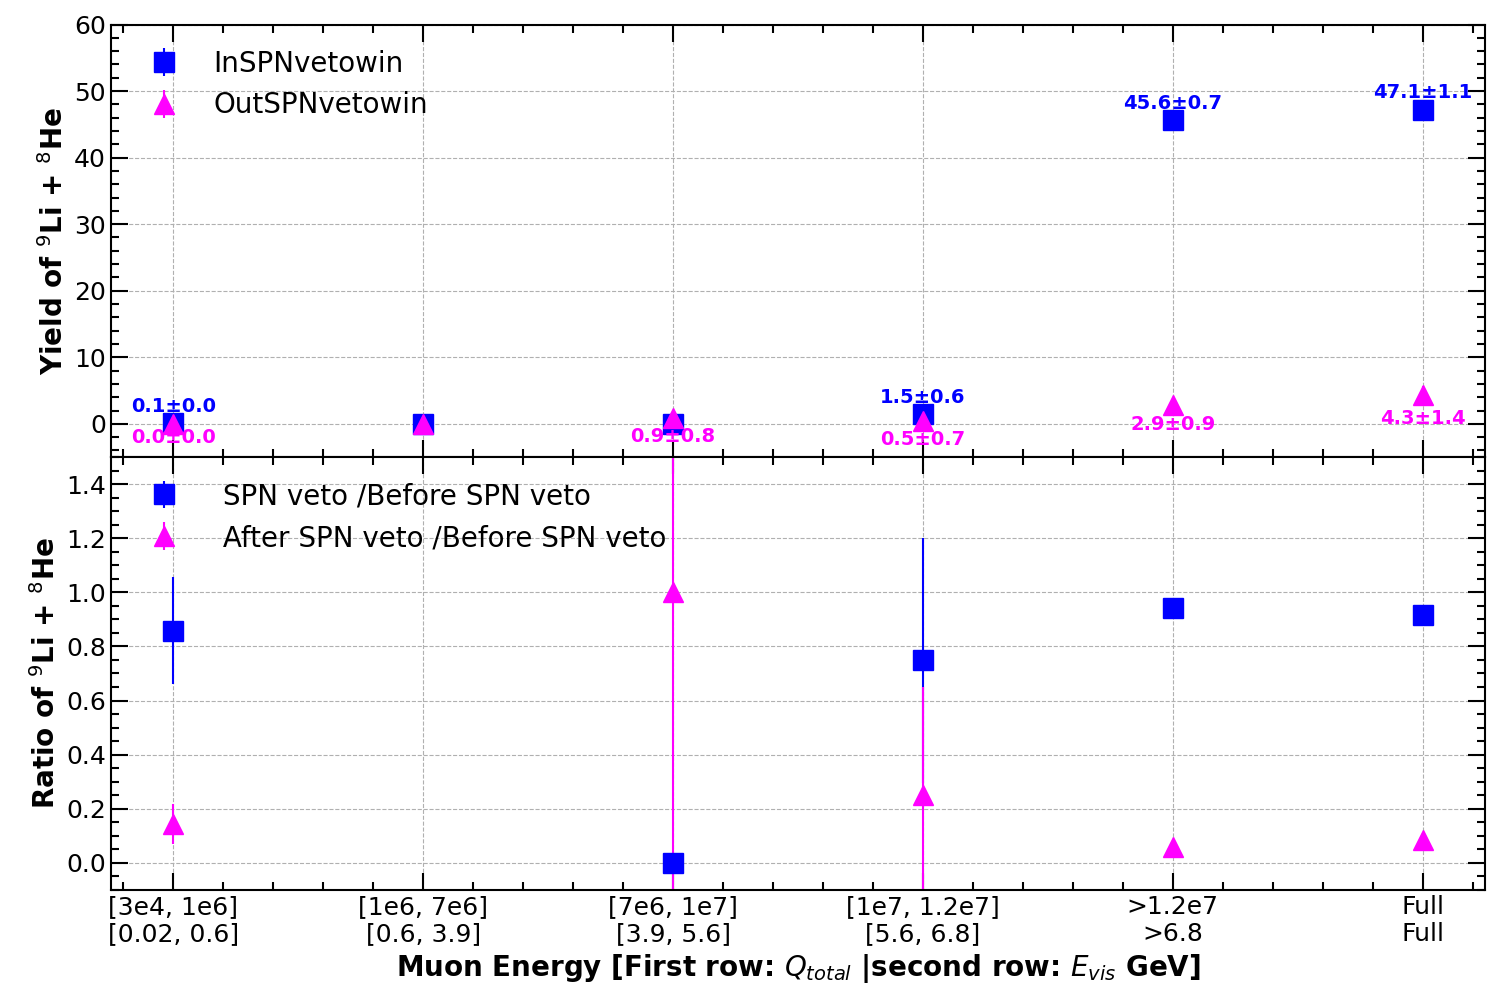
\includegraphics[width=0.8\linewidth]{3_background/spn_veto_rate_summarynew.png}
    \caption{\Li~event rate summary with spn veto.}
    \label{fig:spn_veto_rate_summary}
\end{figure}


% \begin{table}[!htbp]
%     \caption{\Li rate summary after spallation neutron veto.}
%     \label{tab:li9_after_veto}
%     \centering
%     \begin{tabular}{c|cccc}
%         \hline
%         Muon energy [PE] & $<$5e6 & [5e6, 1e7] & [1e7, 2e7] & $>$2e7 \\
%         \hline
%         Livetime [day] & \multicolumn{4}{c}{33.1} \\
%         \hline
%         Counts      & 17$\pm$23  & 71$\pm$42  & 80$\pm$56  & 35$\pm$17  \\
%         Rate [cpd]  &   &   &   &   \\
%         Rate [cpd]  & \multicolumn{4}{c}{6.1$\pm$\td{error from combined fit}} \\
%         \hline
%         Counts (Ep>6 MeV)   & 15$\pm$8  & 23$\pm$14  & 41$\pm$24  & 25$\pm$9 \\
%         Rate [cpd]          &   &   &   & \\
%         \hline
%         Residual [cpd]  &   &   &   &   \\
%         \hline 
%     \end{tabular}
% \end{table}
\subsubsection{MC comparison}
To compare the yields of $^9$Li and $^8$He with those from the GEANT4-v11 simulation, we first establish a calibration between the measured muon visible energy and simulated muon energy loss. Figure~\ref{fig:mueloss} demonstrates that the simulated muon energy loss in the liquid scintillator agrees with the muon visible energy in real data within the energy range of 0.5 GeV to tens of GeV. This agreement is achieved after scaling the simulation by a factor of 1.7$\times$10$^6$ photoelectrons per GeV to obtain the total charge. Using this established relationship and applying the same veto  strategy in the simulation, we then determined the yields for $^9$Li and $^8$He.
\begin{figure}
    \centering
    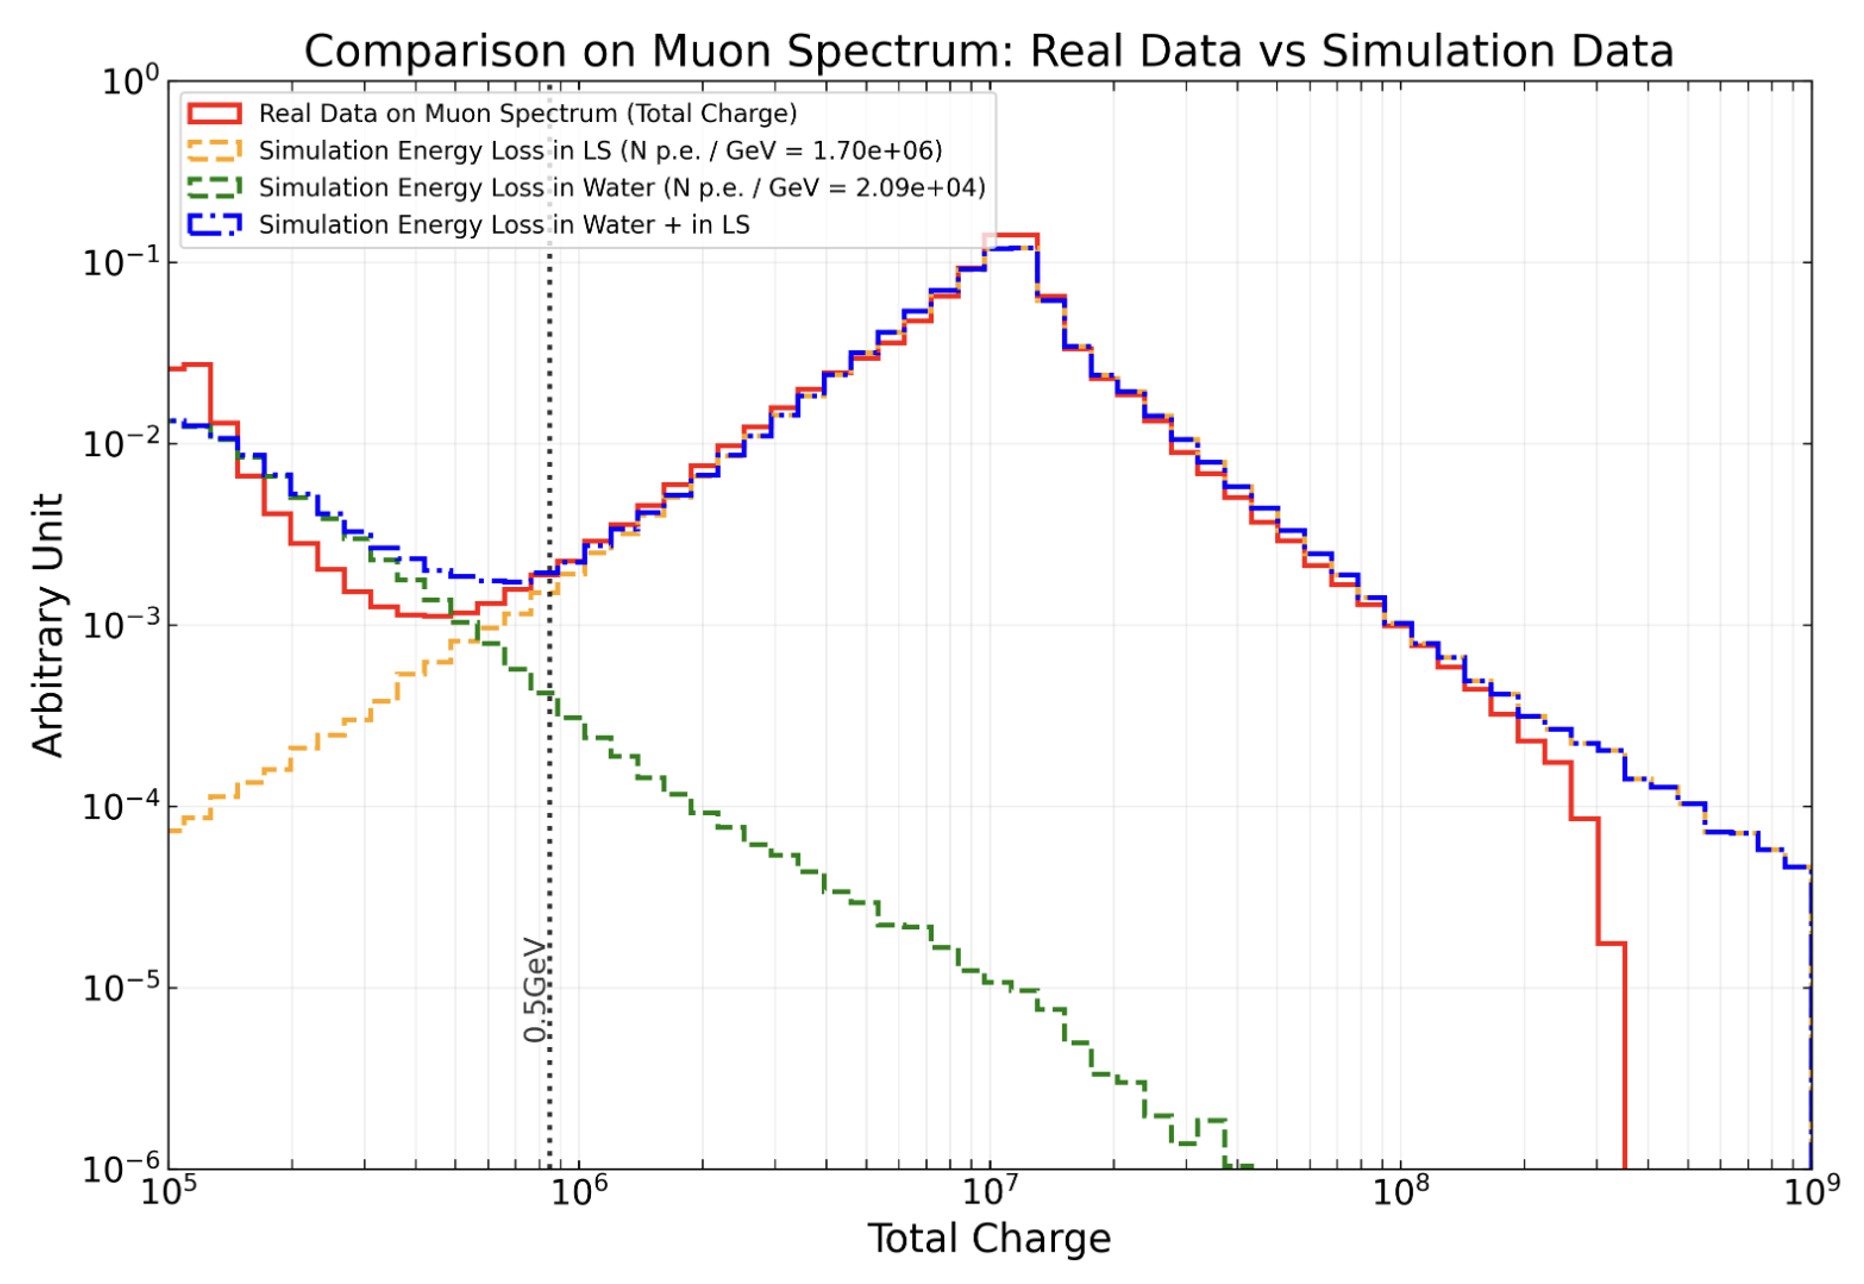
\includegraphics[width=0.8\linewidth]{3_background/muonEloss.png}
    \caption{The simulated muon energy loss in the liquid scintillator matches the muon visible energy in real data well.}
    \label{fig:mueloss}
\end{figure}

Figure~\ref{fig:li9mc} compares the yields of both residual and total $^9$Li and $^8$He from the MC and real data after applying corrections for detector efficiency and muon rate. The residual yields in the IBD sample show good agreement between the simulation and data.
\begin{figure}
    \centering
    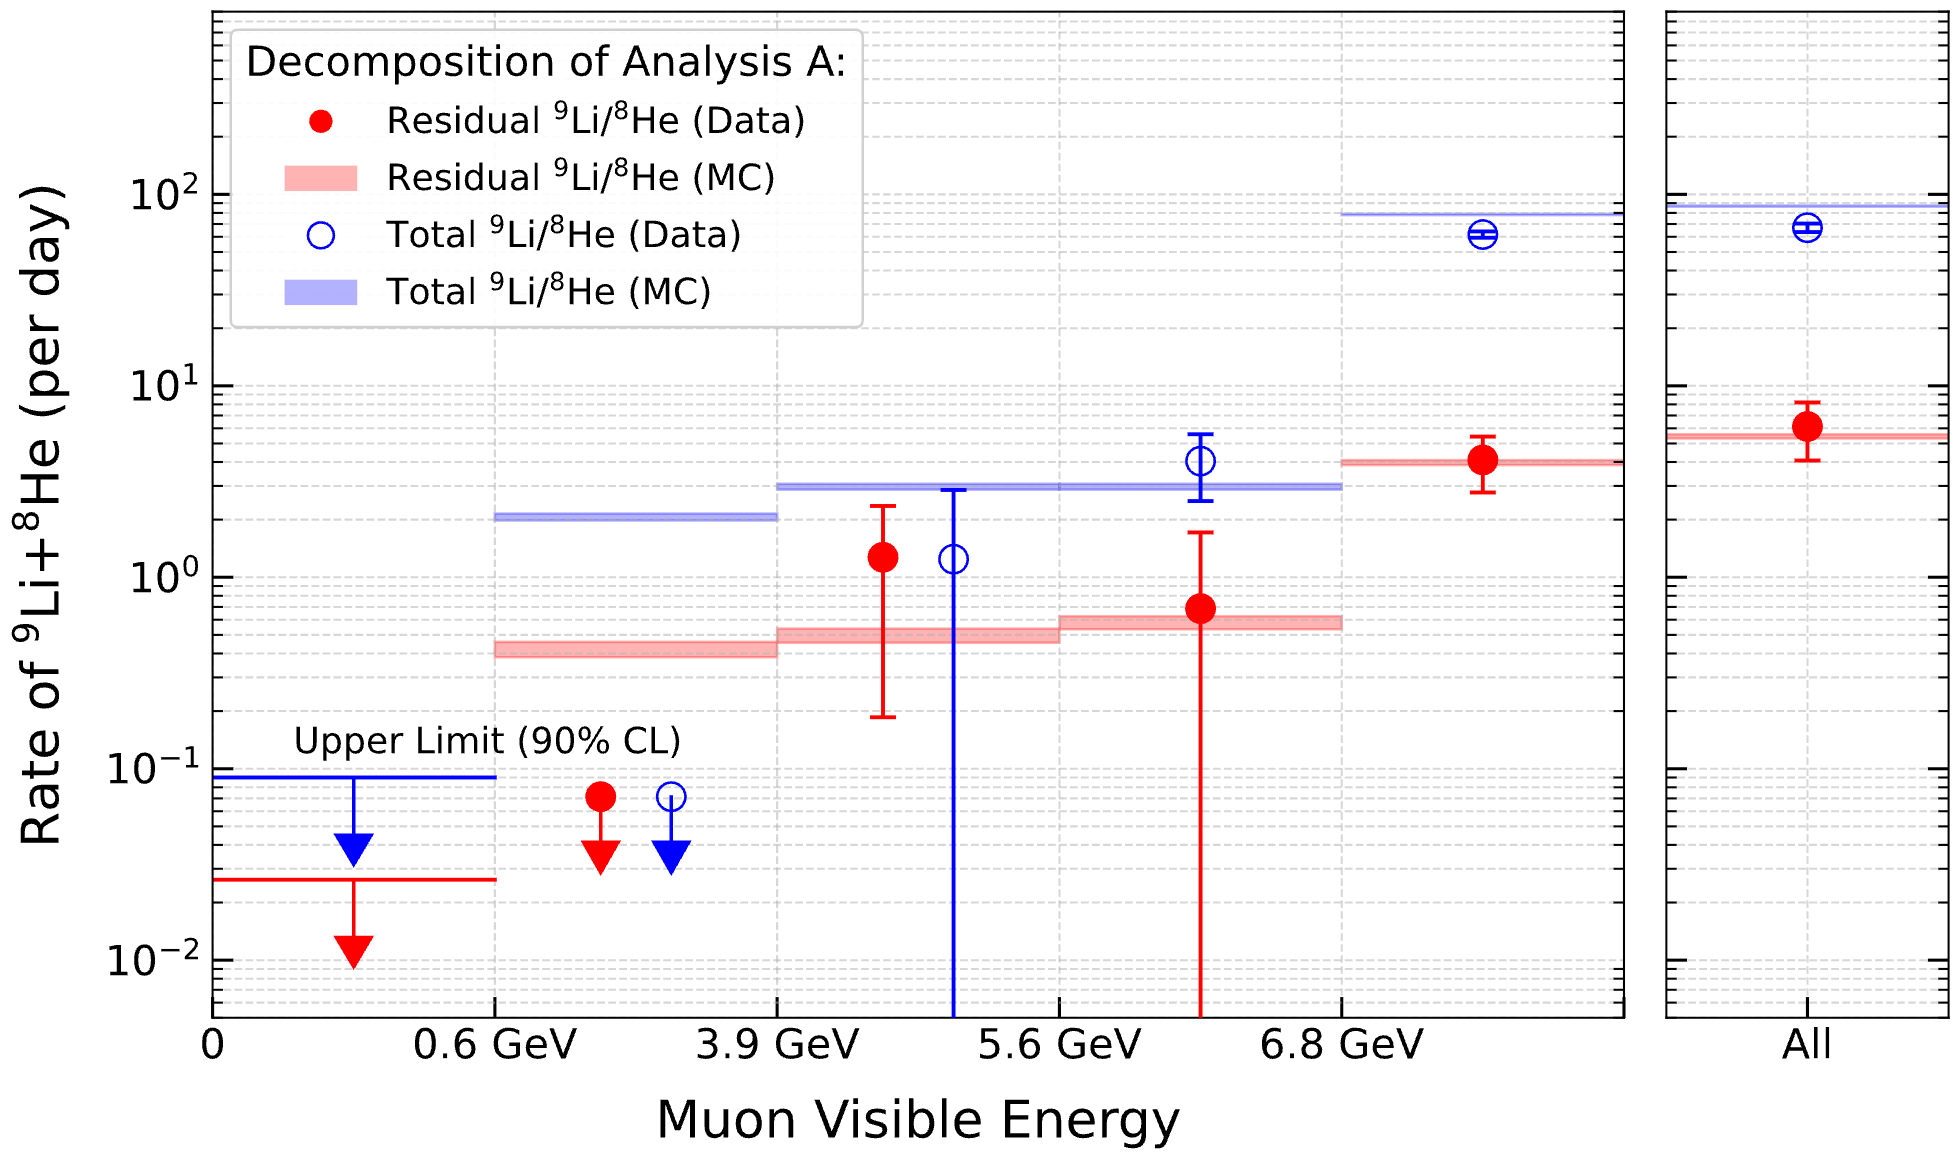
\includegraphics[width=0.8\linewidth]{3_background/li9mc.png}
    \caption{ The comparison of the simulation and real data for the yields of $^9$Li and $^8$He.}
    \label{fig:li9mc}
\end{figure}

\subsubsection{Energy Spectrum}

$^{9}$Li/$^{8}$He energy spectrum can be measured from data in-situ, using SPN-correlated sample. The results are shown in Figure~\ref{fig:li9_spec}, which the corresponding muon energy is $>$ 1.2$\times$10$^7$ pe. Figure~\ref{fig:li9_spec} shows the measured and different predicted energy spectrum. In the left plot, differences between the data and models are presented. A new theoretical modeling of $^9$Li spectrum is proposed in \cite{li9_spec}, and shown in Figure~\ref{fig:li9_spec}. It takes special account into the distribution of the excited states of the intemediate $^9$Be, $^5$He and $^8$Be. These differences are generally small, with deviations of < 20\% for most data points. Additionally, statistical fluctuations dominate the observed discrepancies.
% The measured data spectrum have a reasonable agreement with the predictions above 6 MeV. A clear discrepancies around 3 MeV are  shown for different predictions. 

The right plot presents a comparison of the predicted energy spectra for $^{9}$Li/$^{8}$He from different models. The relative differences between these spectra are generally < 20\%, except energies below 2 MeV, where the discrepancy originates from the DYB2023 model. Finally, through the synthesis of data-model comparisons and inter-model comparisons, the overall uncertainty is determined to be 20\%.
 % The nominal $^9$Li spectrum for the fit will be based on CZ's modeling, constrained by the spn tagged data. The shape error will take into account the difference from data and the several models. The detailed implementation is in progress.
\begin{figure}
    \centering
    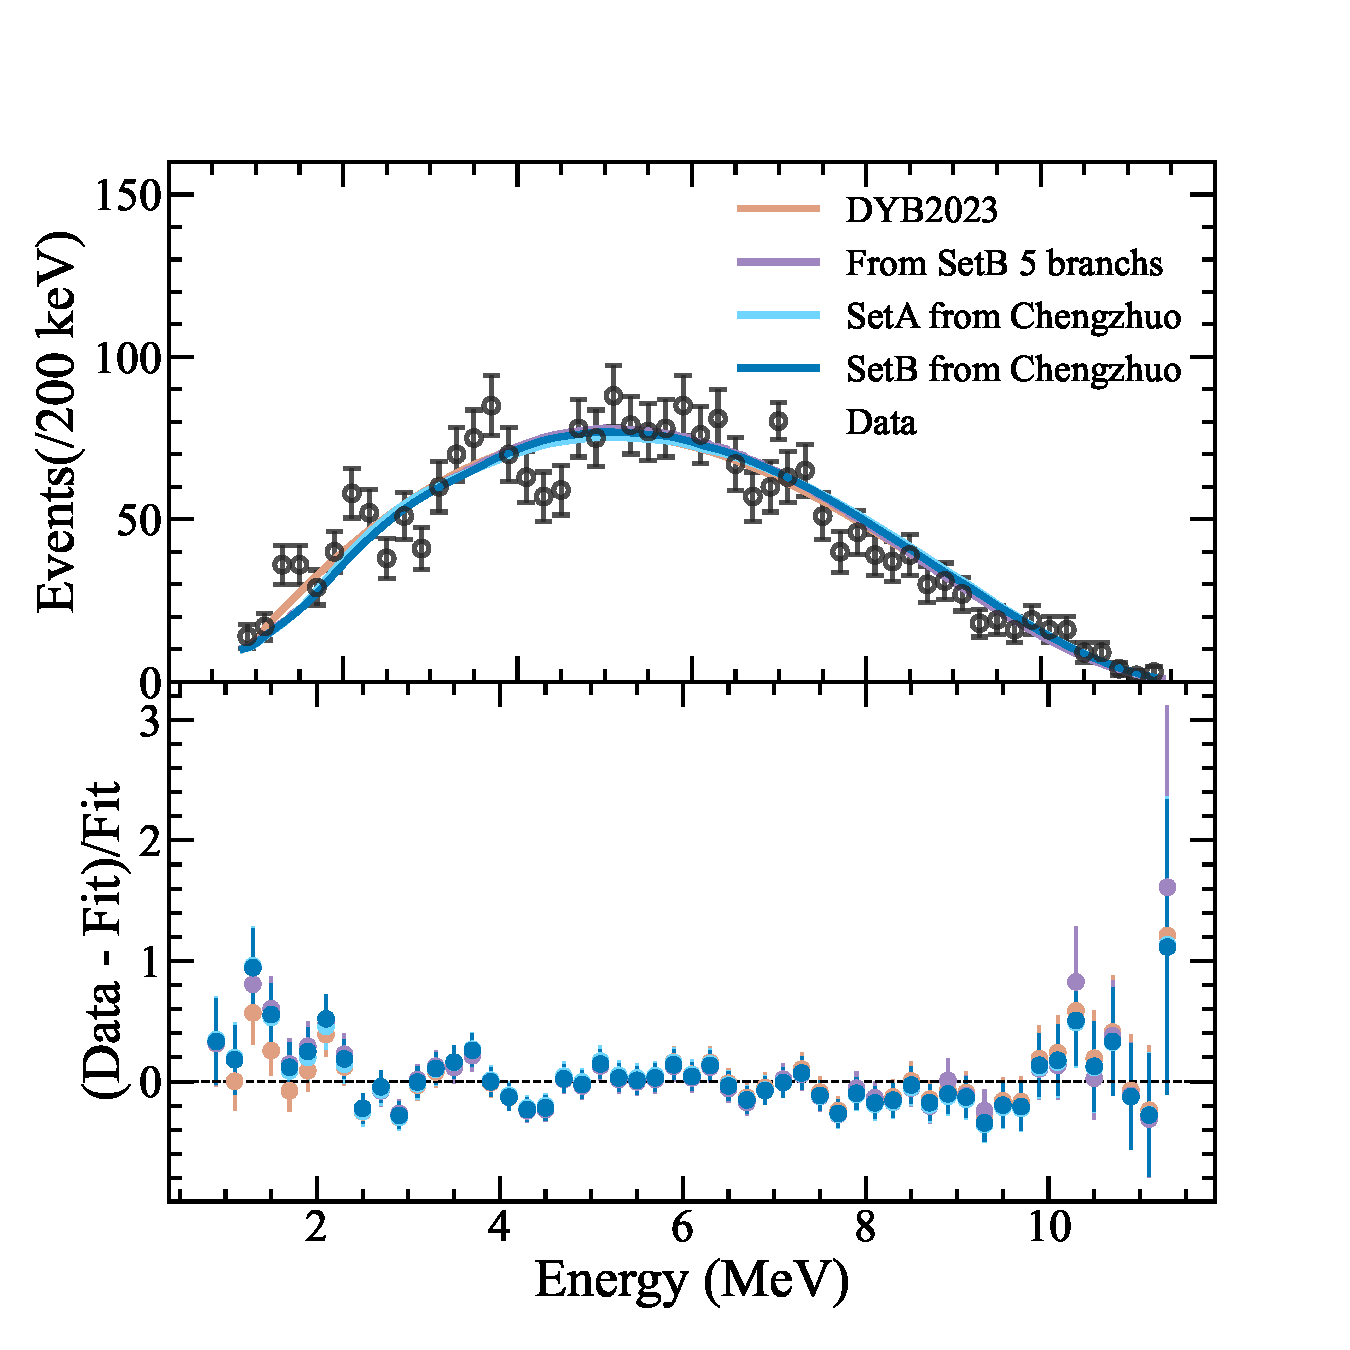
\includegraphics[width=0.45\linewidth]{3_background/Li9energyspectra_comdatamodels.pdf}
    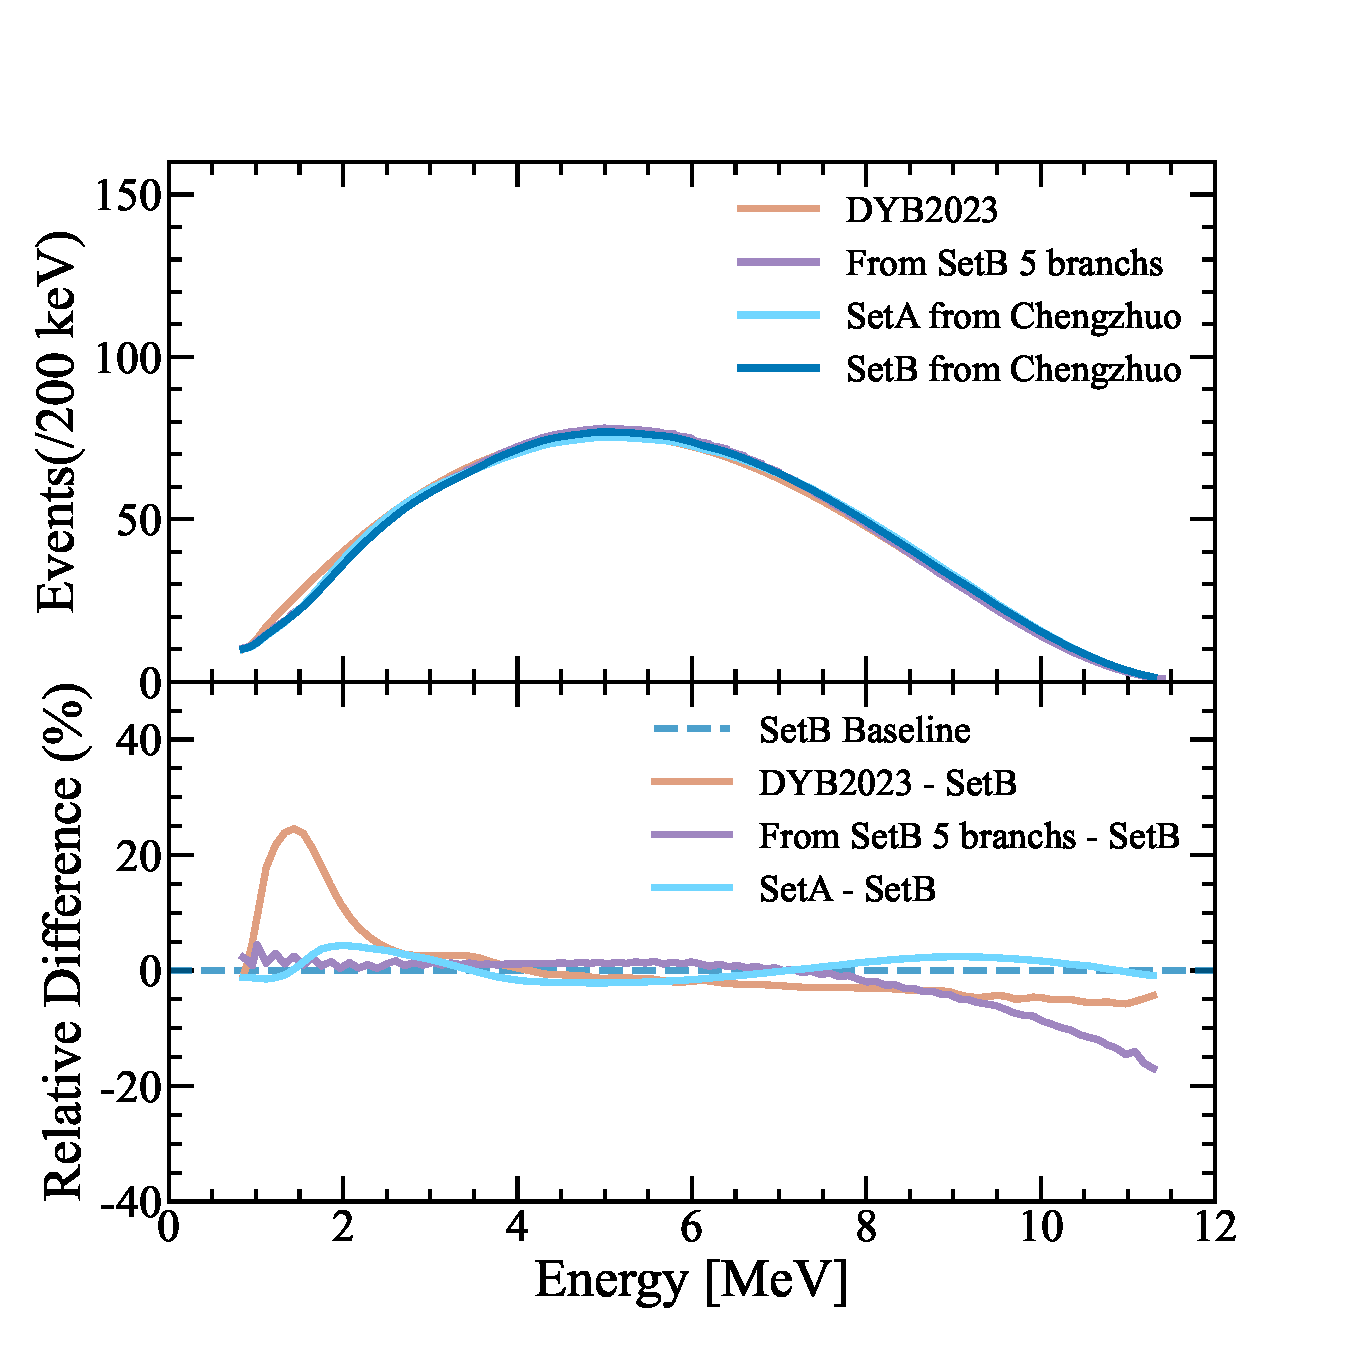
\includegraphics[width=0.45\linewidth]{3_background/Li9energymodelcompare.pdf}
    \caption{$^{9}$Li/$^{8}$He spectrum measured from data and predictions. The measured energy spectrum is tagged by high energy muon with energy larger than 1.2e7 pe, which gives a high purity sample. The left plot shows the results of data and three models. The right plot are predictions from the DYB2023 and sets from Chengzhuo. Model differences are presented in the lower panel of the right plot.}
    \label{fig:li9_spec}
\end{figure}

% \begin{figure}
%     \centering
%     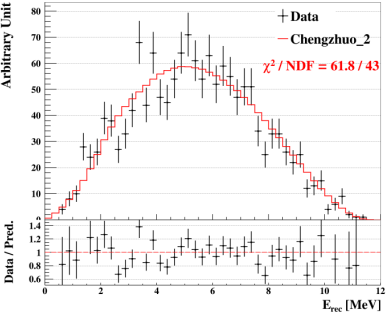
\includegraphics[width=0.6\linewidth]{3_background/li9_CZ.png}
%     \caption{Comparison of the $^9$Li spectrum tagged with spn and the new prediction from Chengzhuo.}
%     \label{fig:li9_CZ}
% \end{figure}

\subsection{Fast neutrons/double neutrons}

  Energetic neutrons generated by cosmic-ray muons represent a background in the JUNO experiment, mainly through two distinct mechanisms: single fast neutrons and double neutron captures. Fast neutrons can imitate an Inverse Beta Decay (IBD) event via elastic scattering off a proton (producing a prompt signal) followed by capture on hydrogen (yielding a delayed signal). Similarly, double neutrons constitute a correlated background in which a muon produces two separate neutrons that are subsequently captured, generating a prompt-like signal from the first neutron’s capture and a delayed signal from the second.
\subsubsection{Rate}
This study employs a comprehensive methodology that integrates Monte Carlo simulations with real-data analysis. The fast neutron selection cut used: prompt energy[0.7,12]MeV, delay energy[2.1,2.5]MeV, prompt signal time [0,2us] from last muon, prompt and delay signal time difference [1,1500]us. The Fidual volume (FV) cut, R<16.5 and |Z|<15.5m. One Monte Carlo dataset(1168-day MC data), containing only rock muons was used, yielding a fast-neutron rate of approximately 0.02/day and a double-neutron rate of 0.05/day, with a total rate below 0.1/day. The spectrum is shown in Figure~\ref{fig:fastn}. Both fast and double-neutron backgrounds are found to be strongly concentrated near the detector’s periphery, rendering them highly sensitive to the fiducial volume cut. Given the low statistical counts for both fast neutrons and double neutrons, a conservative uncertainty of 100\% has been assigned to the rate evaluation.A fast-neutron rate of approximately 0.02$\pm$0.02/day and a double-neutron rate of 0.05$\pm$0.05/day, 
 
\begin{figure}[h]
    \centering
    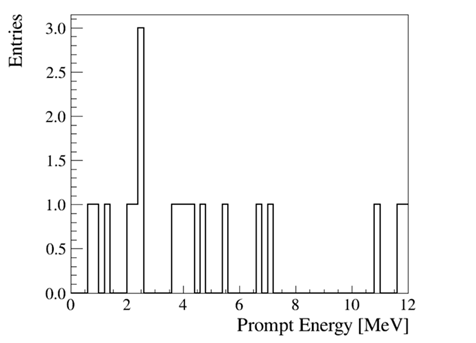
\includegraphics[width=8cm]{3_background/fastn-prompt.png}
    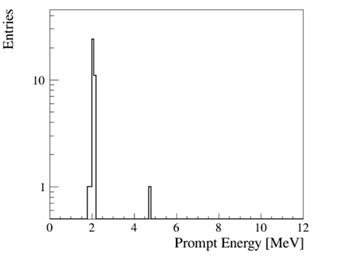
\includegraphics[width=8cm]{3_background/doublen_prompt.png}
    \caption{The prompt energy spectrum for fast neutron(Left figure) and double neutron(Right figure) from MC}
    \label{fig:fastn}
\end{figure}


% \begin{figure}[h]
 %   \centering
 %   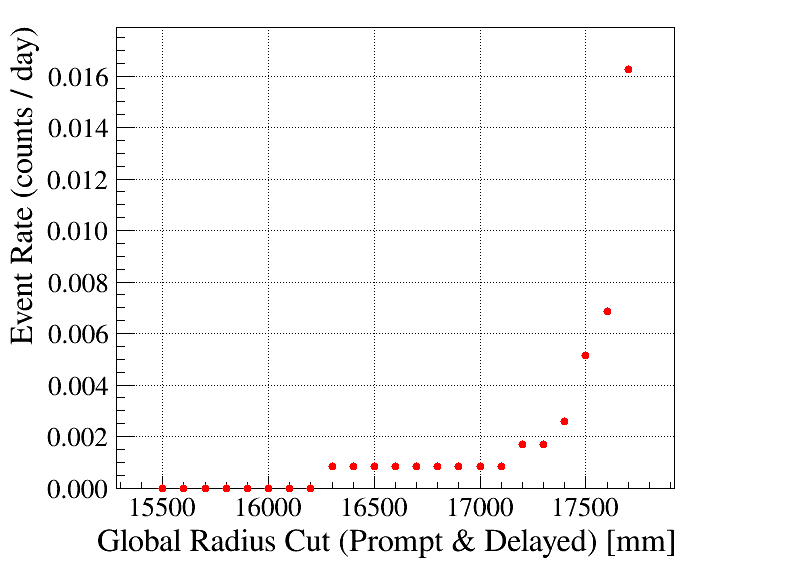
\includegraphics[width=8cm]{3_background/fastn-R.png}
 %   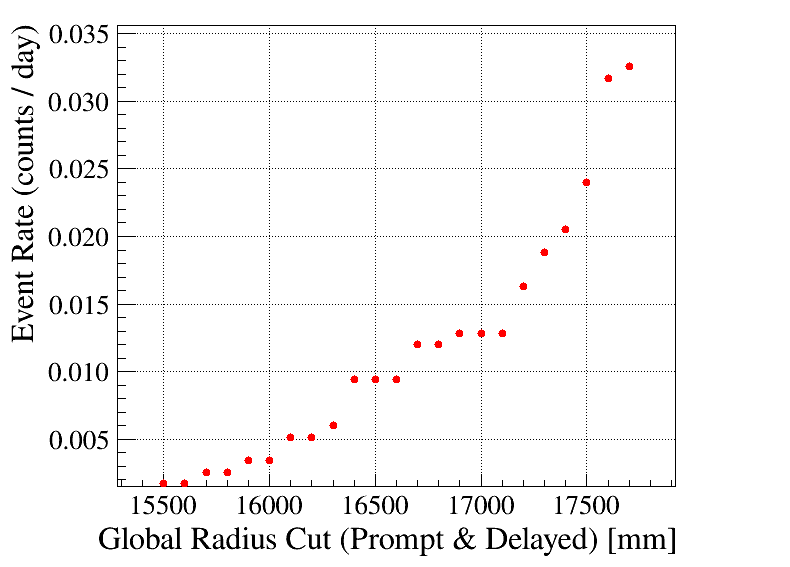
\includegraphics[width=8cm]{3_background/doublen-R.png}
 %   \caption{fast neutron(Left figure) and double neutron(Right figure) background vs detector radius}
 %   \label{fig:fastnR}
%\end{figure}
 

To validate and enrich these findings, real data are employed. A dedicated sample of corner-clipping muons from the Water Pool (with WP PE < 1000 and nHit > 250) is selected to estimate background levels. In an initial dataset spanning ~61 days, 1 fast neutron candidate was observed, while 4 double-neutron candidates were identified. For double neutrons, the expected coincidence events from IBD and Li9 decays within the selection window amount to approximately 4 event. Thus, no significant double-neutron background is observed during this data-taking period. 

\subsubsection{Spectrum}      
   For the energy spectrum study, since both the MC and data statistics are not enough. we intend only to select the high-energy neutrons energy deposited(proton recoil) spectrum to get more statistics, and only select the energy deposited with [0,2us] and FV<16.9 m without other cuts. Since the low statistics, we use a flat fit function to describe the fast-n spectrum.
  For the double neutron prompt signal spectrum from a neutron capture, we'll use the IBD delay signal neutron capture spectrum. The prompt energy spectrum for fast neutron and double neutron will be used, as shown in Fig.~\ref{fig:fastN-spectrum}. 
  
  The energy spectrum uncertainty of fast neutrons was evaluated by comparing the results from a constant linear fit and a first-order polynomial fit, with the discrepancy between these two functions yielding a conservative uncertainty estimate of 60\%. For the double neutron spectrum, the peak shifter error of the calibration source located inside the detector was less than 1\%. By shifting the entire spectrum upward and downward by 1\% and comparing it with the original spectrum, an approximate uncertainty of 50\% was derived.
   \begin{figure}[h]
    \centering
    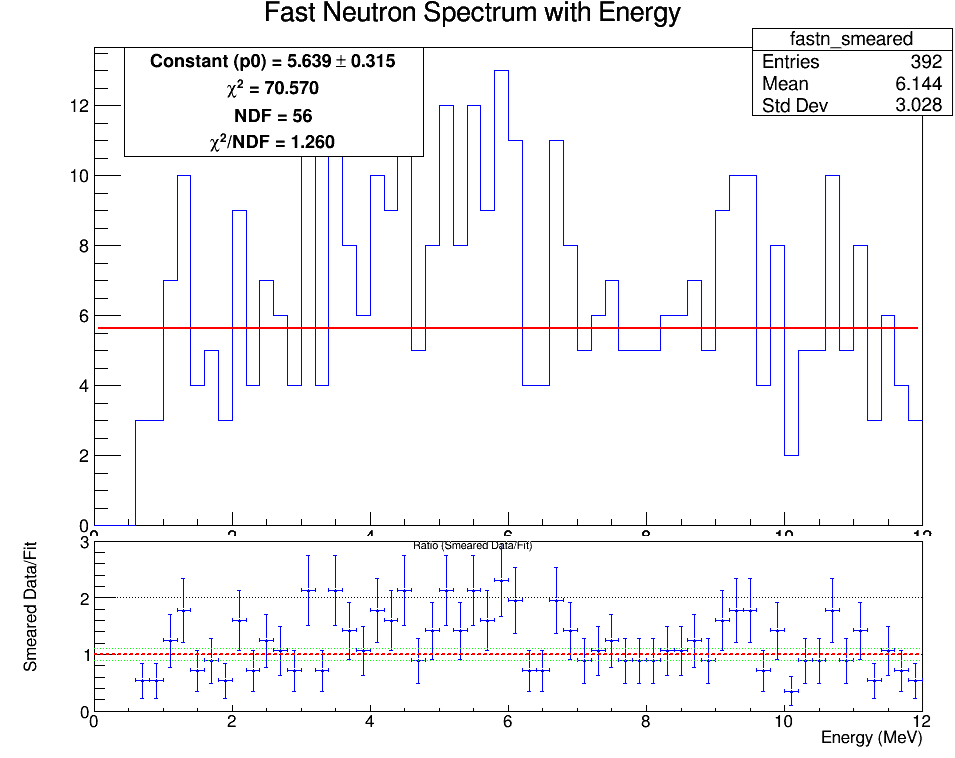
\includegraphics[width=7cm]{3_background/fastn_PromptSpectrum.png}
    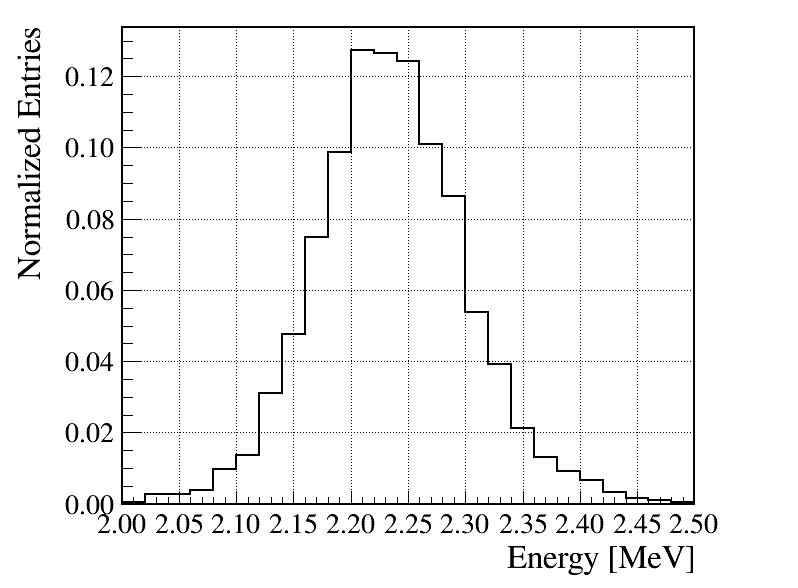
\includegraphics[width=8cm]{3_background/doublen_promptSpectrum.png}
    \caption{fast neutron prompt energy spectrum(Left figure) and double neutron prompt energy spectrum(Right figure) }
    \label{fig:fastN-spectrum}
\end{figure}
 

\subsection{Double $^{12}$B and other potential cosmogenic isotopes}
Cosmogenic isotopes produced by muons traversing the detector, constitute a significant background in IBD analyses. These isotopes are predominantly generated in proximity to muon tracks, often accompanied by neutron production due to muon-induced spallation. The temporal and spatial correlation among isotopes originating from the same muon event enables their effective identification as correlated pairs. In this section, we systematically investigate all potential cosmogenic isotopes that contribute to correlated pair formations (see DocDB: 14926), followed by a discussion of additional $\beta$--$n$ background (see DocDB: 14951) beyond the previously studied $\mathrm{^{9}Li}$ and $\mathrm{^{8}He}$.

\subsubsection{Observation of correlated events in extened delayed-energy window}
\begin{figure}[htbp]
		\centering
		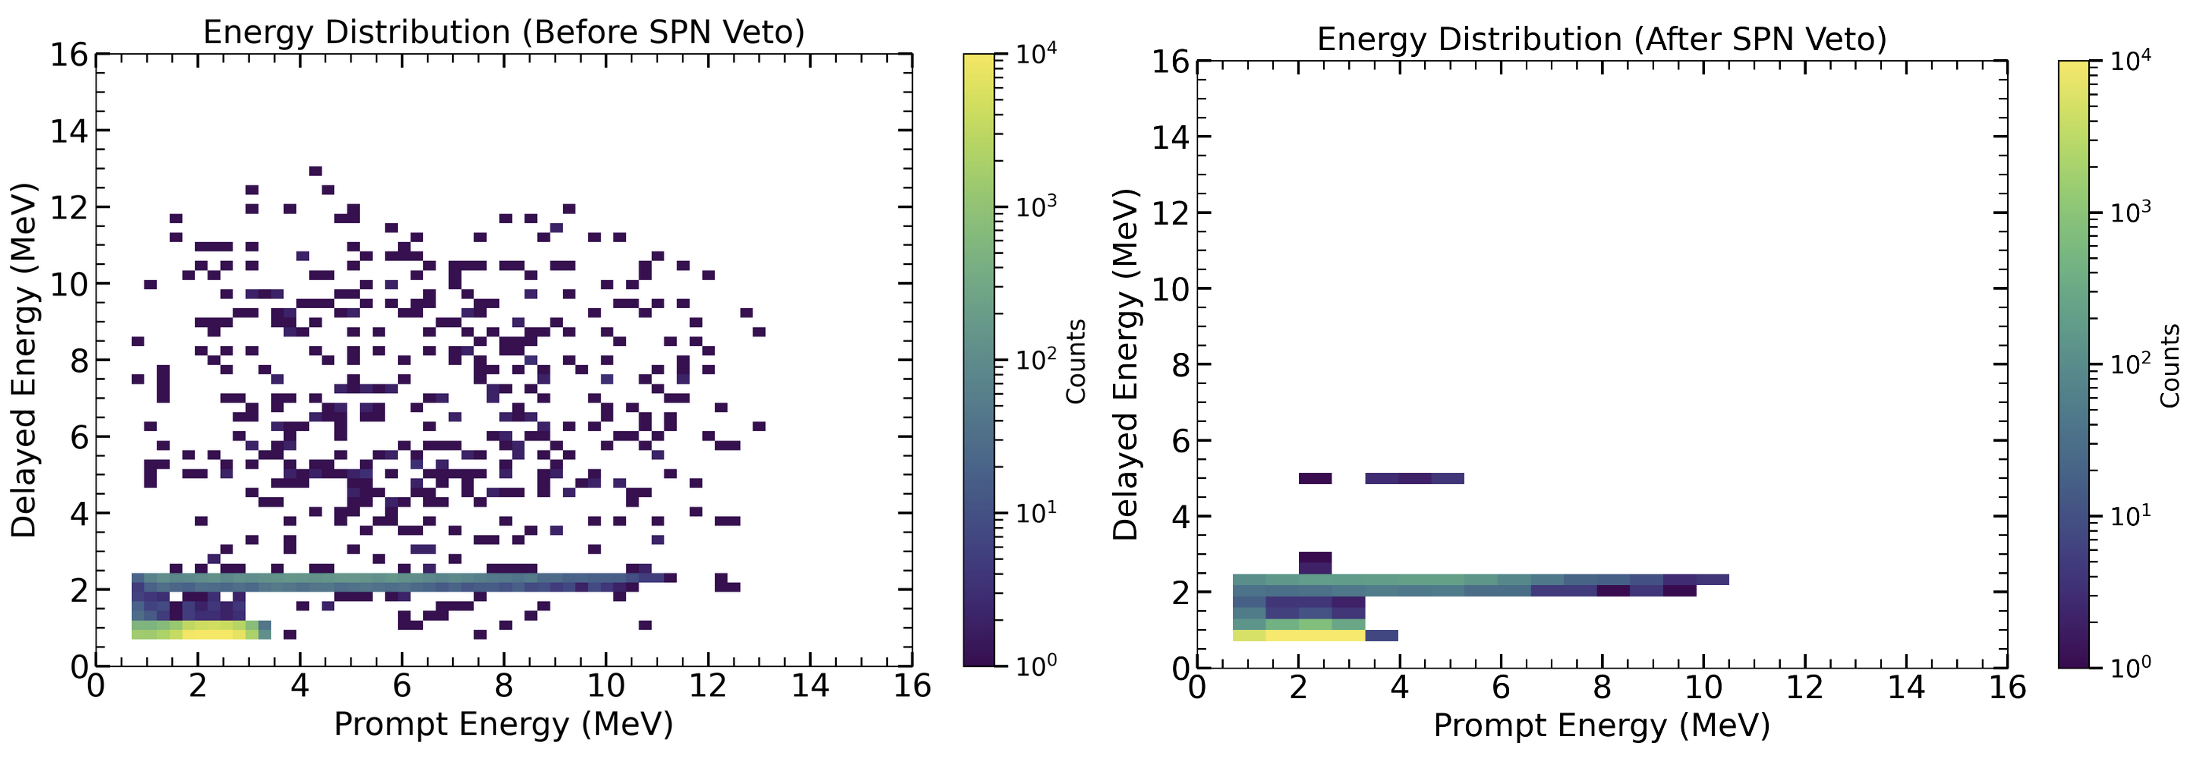
\includegraphics[width= 0.80\columnwidth]{3_background/B12extendeddelayed.png}
		\caption{During the IBD selection process, expanding the energy window for delayed signals reveals additional correlated events with delayed energies exceeding 3 MeV. We observe a reduction in correlated events exhibiting delayed energies exceeding 3 MeV after SPN veto compared to the previous analysis, attributable to the inclusion of muon information from bad files.}
        \label{fig:extendde}
\end{figure}
When the delay energy window in the IBD selection is extended, additional correlated events with delayed energies exceeding 3~MeV become observable, as illustrated in Figure~\ref{fig:extendde}. These events can mimic genuine IBD signals within the neutron capture energy region, necessitating a combined analysis of simulation and experimental data to accurately extrapolate the background rate.
\subsubsection{Paired particle types with $\mathrm{^{12}B}$}
Based on the observed production rates, energy spectra, and lifetimes, the majority of these correlated events before SPN veto are attributed to $\mathrm{^{12}B}$. In this study, we concentrate primarily on $\mathrm{^{12}B}$, with other isotopes addressed in subsequent analyses. To ensure consistency between simulation and experimental data, identical selection criteria are applied in the simulation, including a 5 ms muon veto window, pairing cuts, and multiplicity cuts. 


Figure~\ref{fig:b12time} shows the comparison of real data and MC results for the time difference relative to muons. Red points represent real data obtained from the delayed signal delay time to the closest muon, and are in good agreement with the blue MC points corresponding to pairs involving $\mathrm{^{12}B}$. Purple points denote double $\mathrm{^{12}B}$ events, while yellow points denote pairs involving $\mathrm{^{12}B}$ with other particle components. The lifetime extraction from fits to the comprehensive $\mathrm{^{12}B}$ dataset (green points) yields 29{ms}, aligning with the expected value. However, its production rate in simulation is notably lower than that in real data, suggesting the need for improved calibration of muon induced isotope yields.

\begin{figure}[htbp]
		\centering
		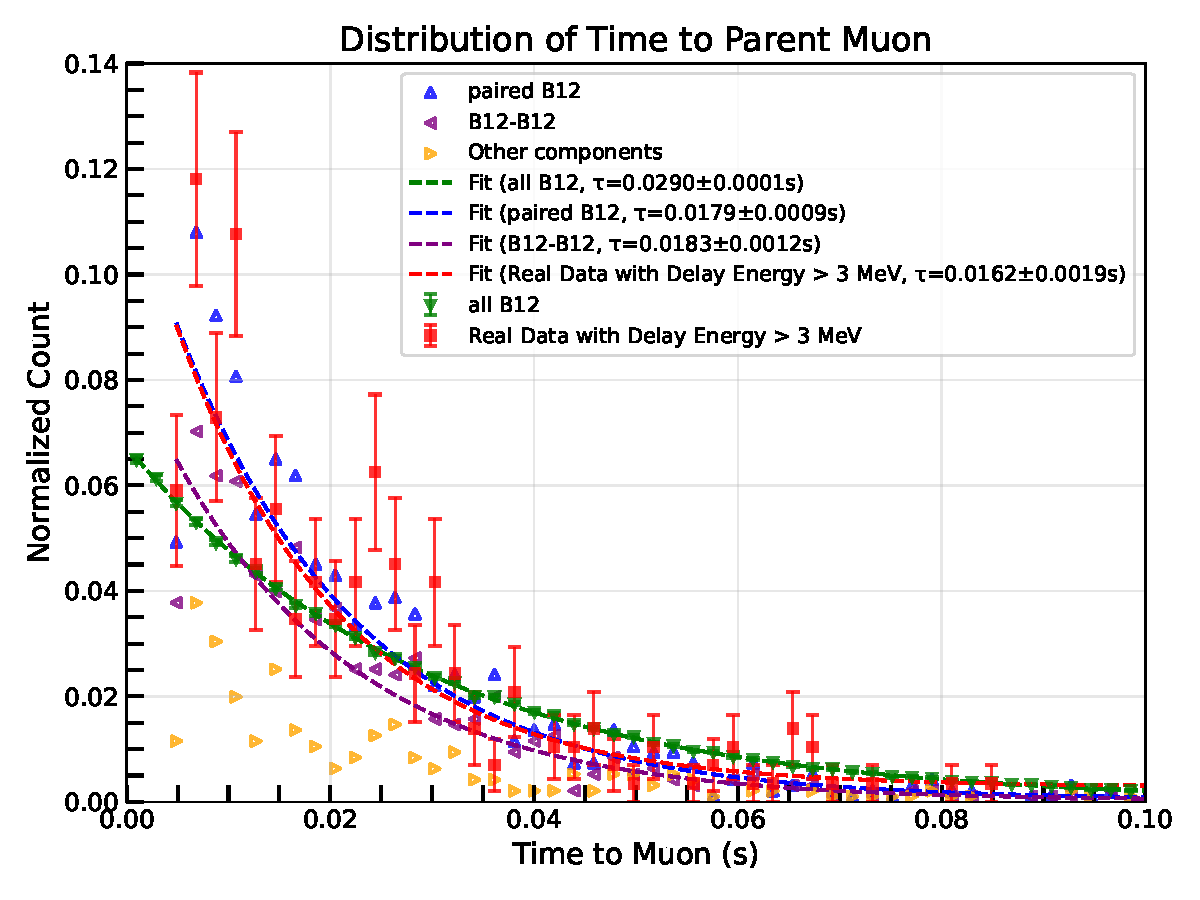
\includegraphics[width= 0.60\columnwidth]{3_background/B12t2mu.pdf}
		\caption{Comparison of time differences relative to the parent muons between the data and MC. Red points correspond to data, obtained from the delayed signal with respect to the nearest muon in time. Blue points correspond to pairs with B12 in the simulation. Purple points denote double-B12 events (B12–B12 pairs) in the MC, while yellow points represent pairs containing other particle components; both purple and yellow points are normalized to the count of blue-marked paired events. Green points show all B12 data in the MC, normalized to its total count.}
        \label{fig:b12time}
\end{figure}


\begin{table}[htbp]
\centering
\begin{tabular}{|l|c|c|}
\hline
\textbf{Paired particle with $\mathrm{^{12}B}$} & \textbf{Paired rate before spn veto(cpd)} & \textbf{Proportion} \\
\hline
$\mathrm{^{12}B}$   & 5.10 & 69.9\% \\
\hline
$\mathrm{^{12}N}$   & 1.03 & 14.2\% \\
\hline
$\mathrm{^{9}C}$    & 0.39 & 5.4\% \\
\hline
$\mathrm{^{8}Li}$   & 0.26 & 3.6\% \\
\hline
$\mathrm{^{6}He}$   & 0.21 & 2.8\% \\
\hline
$\mathrm{^{8}B}$    & 0.21 & 2.9\% \\
\hline
$\mathrm{^{10}C}$   & 0.03 & 0.4\% \\
\hline
$\mathrm{^{11}C}$   & 0.02 & 0.2\% \\
\hline
$\mathrm{^{9}Li}$   & 0.02 & 0.3\% \\
\hline
$\mathrm{^{8}He}$   & 0.02 & 0.2\% \\
\hline
neutron             & 0.01 & 0.1\% \\
\hline
$\mathrm{^{11}Be}$  & 0.00 & 0.0\% \\
\hline
$\mathrm{^{16}N}$   & 0.00 & 0.0\% \\
\hline
\textbf{Total}      & \textbf{7.27} & \textbf{100\%} \\
\hline
\end{tabular}
\caption{Paired particle types with $\mathrm{^{12}B}$ and their contributions before SPN veto over a 150-day Geant4-10 simulation sample.}
\label{tab:b12}
\end{table}


Table~\ref{tab:b12} summarizes the particle types paired with $\mathrm{^{12}B}$ in a 150-day simulation sample. After scaling to match the muon rate observed in real data, the total pairing rate is approximately 7.3 cpd, with the majority of paired signals consisting of double $\mathrm{^{12}B}$ combinations.
\subsubsection{Correlated events including all potential cosmogenic isotopes}
\begin{table}[htbp]
\centering
\begin{tabular}{|l|c|c|}
\hline
\textbf{Paired Particle} & \textbf{Rate before spn veto (cpd)} & \textbf{Rate after spn veto (cpd)} \\
\hline
$\mathrm{^{12}B}$ & 9.99 (7.27) & 0.01 (0.04) \\
\hline
$\mathrm{^{12}N}$ & 1.31 (1.17) & 0.004 (0) \\
\hline
$\mathrm{^{8}Li}$ & 0.82 (0.66) & 0.08 (0.05) \\
\hline
$\mathrm{^{9}C}$ & 0.17 (0.51) & 0 (0) \\
\hline
$\mathrm{^{6}He}$ & 0.92 (0.43) & 0.08 (0.02) \\
\hline
$\mathrm{^{8}B}$ & 0.12 (0.37) & 0.02 (0.02) \\
\hline
$\mathrm{^{10}C}$ & 0.18 (0.15) & 0.06 (0.06) \\
\hline
$\mathrm{^{11}C}$ & 0.11 (0.03) & 0.08 (0) \\
\hline
$\mathrm{^{9}Li}$ & 0.21 (0.03) & 0 (0) \\
\hline
$\mathrm{^{8}He}$ & 0.04 (0.01) & 0 (0) \\
\hline
Be11 & 0 (0.01) & 0 (0.01) \\
\hline
N16 & 0 (0) & 0 (0) \\
\hline
\textbf{Total} & \textbf{10.92 (8.02)} & \textbf{0.23 (0.15)} \\
\hline
\end{tabular}
\caption{Correlated events rate including all potential cosmogenic isotopes with and without SPN veto over a 277.5-day Geant4-11 simulation sample (150-day Geant4-10 simulation sample in bracket).}
\label{tab:paired_table2}
\end{table}




We extend Table~\ref{tab:paired_table2} to include all potential isotopes, not only B12 in two simulation samples. Before the SPN veto, the total paired rate is 10.92 (8.02) cpd (with 9.99 (7.27) cpd attributed to B12 and Li-9/He-8 neutron pairings not included). After applying the SPN veto, the total is 0.23 (0.15) cpd.
\begin{figure}[htbp]
		\centering
		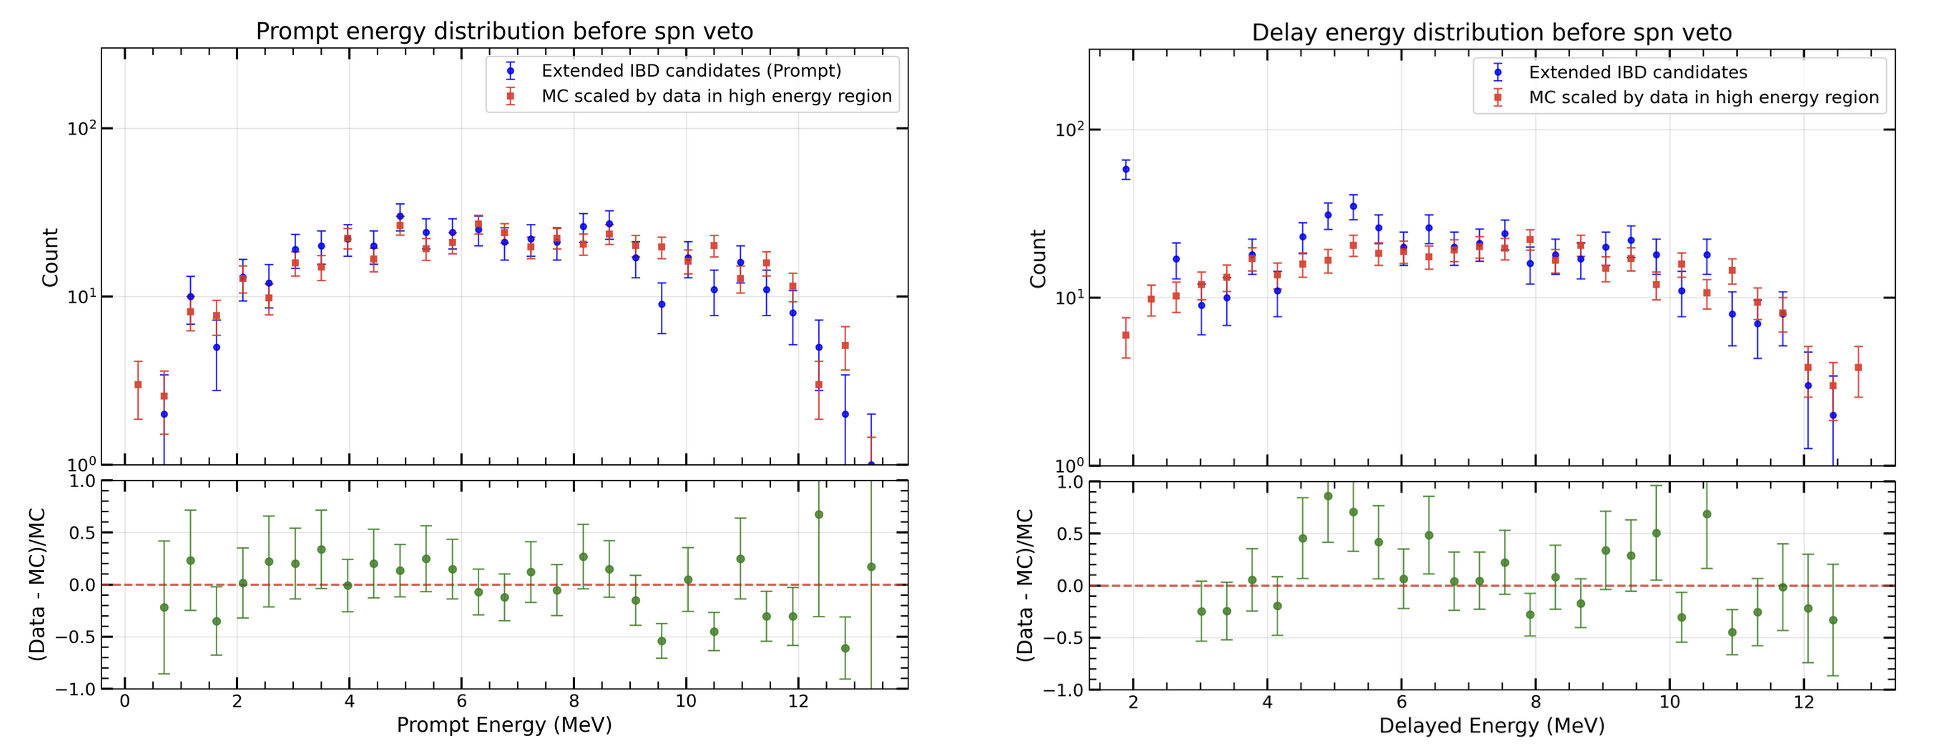
\includegraphics[width= 0.90\columnwidth]{3_background/B12spec.png}
		\caption{Extended delay energy spectrum and prompt energy spectrum for IBD candidates selection in real data (blue) and the scaled MC delay energy spectrum for correlated events from all potential cosmogenic isotopes (red).}
        \label{fig:b12delay}
\end{figure}




Two 59.1-day data samples were analyzed, one incorporating the spn veto and the other excluding it. 
Figure~\ref{fig:b12delay} shows the extended delay energy spectrum for IBD candidates selection (blue); the red curve shows the scaled MC delay energy spectrum for correlated events from all potential cosmogenic isotopes.
To extrapolate the IBD background in the 2.1–2.6 MeV delay energy interval, we employ the rate above 6 MeV threshold to suppress neutron capture events on carbon. 


\begin{table}[htbp]
\centering

\newcommand{\tabletitlewidth}{4.5cm}

\begin{tabular}{|l|c|c|}
\hline
\makebox[\tabletitlewidth][l]{\textbf{Before SPN veto ($\mathrm{E_d}$)}} & \textbf{$>6$ MeV} & \textbf{2.1--2.6 MeV} \\
\hline
G4-10 rate (cpd) & 4.65 $\pm$ 0.19 (stat.) & 0.28 $\pm$ 0.05 (stat.) \\
\hline
G4-11 rate (cpd) & 5.08 $\pm$ 0.14 (stat.) & 0.36 $\pm$ 0.05 (stat.) \\
\hline
Data rate (cpd) & 6.55 $\pm$ 0.40 (stat.) & \textbf{0.46 $\pm$ 0.07 (sys.) $\pm$ 0.11 (stat.)} \\
\hline
\end{tabular}

\vspace{0.3cm} 

\begin{tabular}{|l|c|c|}
\hline
\makebox[\tabletitlewidth][l]{\textbf{After SPN veto ($\mathrm{E_d}$)}} & \textbf{$>6$ MeV} & \textbf{2.1--2.6 MeV} \\
\hline
G4-10 rate (cpd) & 0.04 $\pm$ 0.02 (stat.) & 0.01 $\pm$ 0.01 (stat.) \\
\hline
G4-11 rate (cpd) & 0.04 $\pm$ 0.01 (stat.) & 0.01 $\pm$ 0.01 (stat.) \\
\hline
Data rate (cpd) & $<0.055$ (90\% CL)& \textbf{<0.014  (90\% CL)} \\
\hline
\end{tabular}

\caption{Rates before and after the SPN veto for two energy windows, with the 2.1–2.6 MeV IBD background extrapolated via the Geant4-10 and Geant4-11 simulation derived ratio.}
\label{tab:rates_ED_before}
\end{table}



Before the SPN veto, the rate for delay energy above 6 MeV is 6.55 cpd, slightly higher than the MC prediction as shown in Table~\ref{tab:rates_ED_before}. This difference can be explained by the data showing a $\mathrm{^{12}B}$ production rate higher than the expected rate from MC. Using the simulation derived IBD background ratio yields an extrapolated IBD background rate in data of 0.46 cpd, with a statistical uncertainty of 0.11 cpd, and a systematic uncertainty of 0.07 is estimated by comparing results from different simulation samples. 
After applying the SPN veto, no candidate events are observed. This allows us to establish a 90\% CL upper limit of 0.055 cpd on the signal rate for events with delayed energy > 6 MeV. The 90\% CL upper limit on the corresponding extrapolated IBD background is 0.014 cpd. As this limit is negligible, it was not included in the subsequent analysis.

\subsubsection{Cosmic ray induced ${\beta}$-n isotopes}
Beyond $\mathrm{^9Li}$ and $\mathrm{^8He}$, several $\mathrm{\beta}$-n isotopes produced by cosmic ray spallation can contribute to IBD like backgrounds in JUNO, including $\mathrm{^{11}Li}$, $\mathrm{^{12}Be}$, $\mathrm{^{14}B}$, $\mathrm{^{16}C}$, $\mathrm{^{17}N}$, and $\mathrm{^{18}N}$. For the long lived species such as $\mathrm{^{16}C}$, $\mathrm{^{17}N}$, and $\mathrm{^{18}N}$, their delayed neutron-emitting decays make vetoing by spallation neutrons or  muon track particularly challenging. Consequently, a quantitative assessment of this irreducible background relies on simulation. Using combined FLUKA and Geant4 simulations, we estimate the total $\mathrm{\beta}$-n background from isotopes excluding $\mathrm{^{17}N}$ to be approximately 0.02~cpd with a systematic uncertainty of about 40\%. The $\mathrm{^{17}N}$ $\mathrm{\beta}$-n background rate remains uncertain, as the two simulations differ by roughly an order of magnitude and require further cross-checking. Notably, $\mathrm{^{17}N}$ constitutes the dominant $\mathrm{\beta}$-n background despite the uncertainty, details can be found in DocDB: 14951.


\subsection{$^{13}$C($\alpha$, n)$^{16}$O}
%Done by Rongping.

$\alpha$ from natural radioactivity may interact with a nucleus and emit a neutron. The reaction, formed by X($\alpha$;n)Y, introduces background to the LS based neutrino experiments. In the LS detector, $\alpha$ comes from $^{238}$U, $^{232}$Th, and $^{210}$Po decay chains. The nucleus $^{13}$C is a natural component of Carbon which is rich in the LS. The $^{13}$C($\alpha$;n)$^{16}$O reaction
forms the correlation as following: the prompt signal is neutron elastic scattering on proton or inelastic scattering on $^{12}$C, and the delayed signal is neutron capture on Hydrogen. If $^{16}$O is in the excited state, de-excitation of $^{16}$O emits  or conversion electron which also contributes to the prompt signal. The signature is the same as $\overline{\nu}_e$, so such events can't be distinguished from $\overline{\nu}_e$ samples. The background rate and spectrum should be subtracted carefully from the neutrino candidates.

\subsubsection{Neutron yield and spectrum}
A newly developed generator code for calculating the alpha-n yield has been developed by Rongping (IHEP), details can be found in Doc14912. The difference of this method to SaG4n (published paper) is that the deposited energy for each step is simulated directly in JUNOSW with default detector parameters and G4 version (Geant4.10.04.p02), while SaG4n is a separate generator built based on Geant4.11.1.2.

A comparison of neutron yield and spectrum between these two methods are shown in Table~\ref{tab:alphaNyield} and Figure~\ref{fig:alphaNspec}. The two results of neutron yield are consistent within the uncertainty of 25\%, while the spectrum has some difference, this will be updated with the new production.

\begin{table}[!htbp]
    \caption{Comparison of alphaN yield from two generators.}
    \label{tab:alphaNyield}
    \centering
    \footnotesize% fontsize
    \setlength{\tabcolsep}{4pt}% column separation
    \renewcommand{\arraystretch}{1.2}%row space 
    \begin{tabular}{c|c|c|c}
        \hline
        Neutron yield & IHEP & SaG4n & Ratio  \\
        
        [count/chain] & (G4.10.04.p02,J24.3.0) & (G4.11.1.2) & (SaG4n/IHEP) \\ \hline
        $^{238}$U & 7.39e-7 & 6.36e-7 & 86\% \\
        $^{232}$Th & 9.44e-7 & 8.58e-7 & 91\% \\
        $^{210}$Po & 6.13e-8 & 5.11e-8 & 83\% \\
        \hline 
    \end{tabular}
\end{table}

In this step, we also get the 2D distrution of neutron kinetic energy and alpha 
deposited energy. This distribution is then sent to JUNOSW for further simulation to get the prompt signal.

\begin{figure}[h]
    \centering
    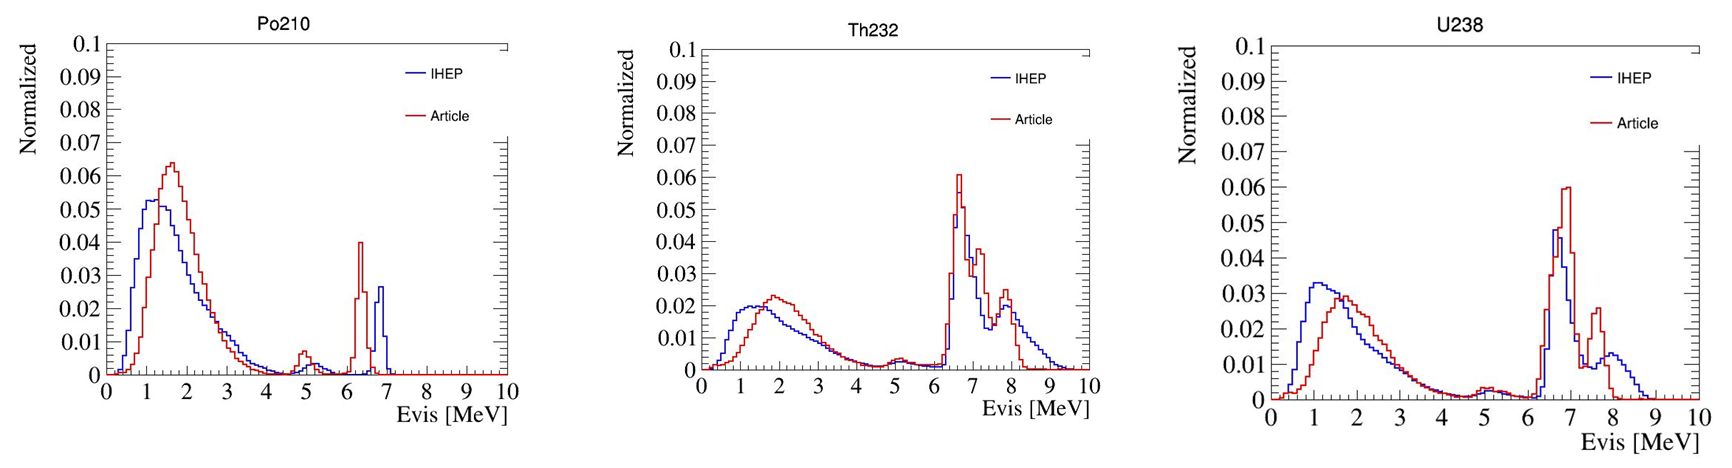
\includegraphics[width=16cm]{3_background/alphaNspec.png}
    \caption{Comparison of alphaN prompt spectrum from two generators.}
    \label{fig:alphaNspec}
\end{figure}

\subsubsection{Alpha rate}
The rates of $^{238}$U, $^{232}$Th are measured by BiPo correlated signal selection, details about the selection methods are described in Doc14623 and Doc14613. The rate of $^{210}$Po is measured by fitting the alpha peak in the total spectrum, details can be found in Doc14616.

The evolution of $^{214}$BiPo and $^{212}$BiPo are shown in Figure~\ref{fig:UTh}. The radon in LS in the begining is high, which lead to higher BiPo rate. The $^{214}$BiPo and $^{212}$BiPo have reached equilibrium states now, and the expected plateau are (7.5$\pm$0.9)$\times$10$^{-17}$ g/g for $^{238}$U and (8.2$\pm$0.7)$\times$10$^{-17}$ g/g for $^{232}$Th.

\begin{figure}[h]
    \centering
    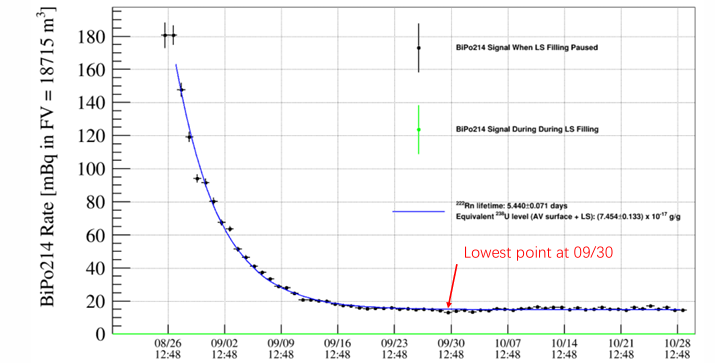
\includegraphics[width=8cm]{3_background/U238_update.png}
    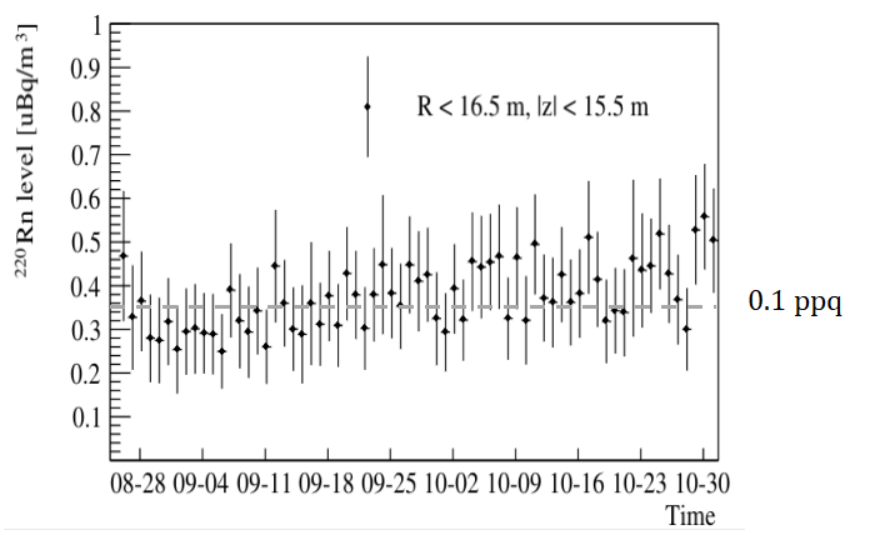
\includegraphics[width=9cm]{3_background/Th232_update.png}
    \caption{The evolution of $^{238}$U and $^{232}$Th within IBD FV cut (R<16.5m, |z|<15.5m).}
    \label{fig:UTh}
\end{figure}



The evolution of $^{210}$Po is shown in Figure~\ref{fig:Po210}. The half-life of $^{210}$Po is 138.376~days, thus the decay is slower and not reach equilibrium at present. The amount of $^{210}$Po was measured at the end of the LS filling at about 5$\times$10$^4$~cpd/kt, decreasing to an average (4.3$\pm$0.3)$\times$10$^4$~cpd/kt over the first two months of science runs.


\begin{figure}
    \centering
    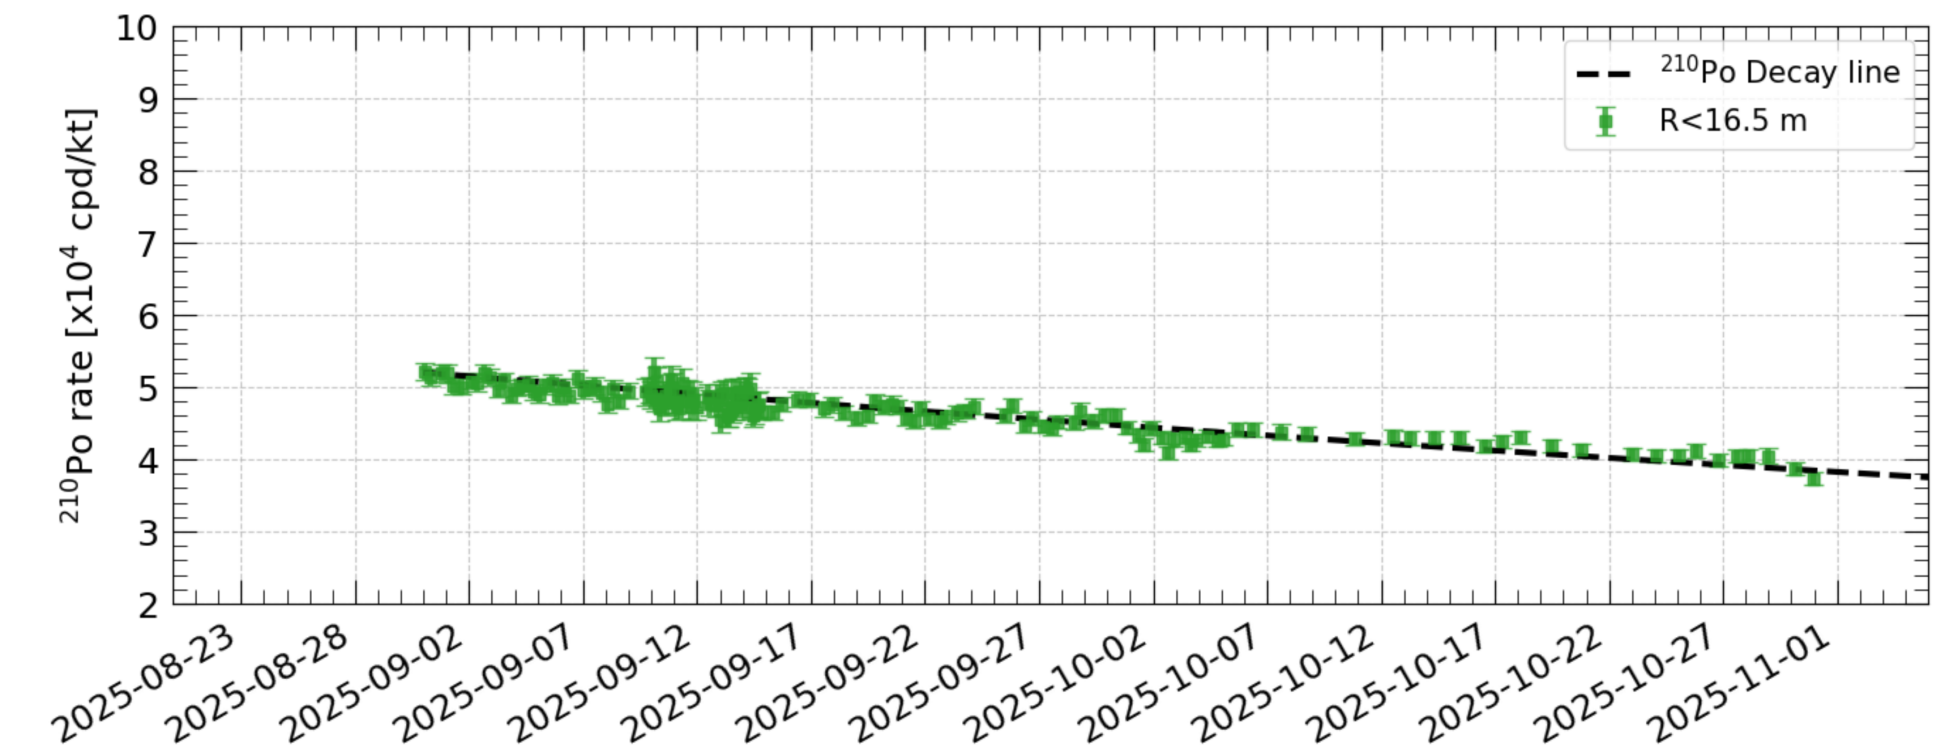
\includegraphics[width=0.75\linewidth]{3_background/Po210_update.png}
    \caption{The evolution of $^{210}$Po within IBD FV cut (R<16.5m).The black dashed line represents the $^{210}$Po decay curve, and its variation trend is quite consistent with that of the rate.  }
    \label{fig:Po210}
\end{figure}

\subsubsection{Final alphaN background rate}
With the calculated neutron yield from Table~\ref{tab:alphaNyield} and measure alpha rate, the final alphaN background rate is summarized in Table~\ref{tab:alphaN}.

% \begin{table}[!htbp]
%     \caption{Final alphaN background rate and uncertainty.}
%     \label{tab:alphaN}
%     \centering
%     \footnotesize% fontsize
%     \setlength{\tabcolsep}{4pt}% column separation
%     \renewcommand{\arraystretch}{1.2}%row space 
%     \begin{tabular}{c|cc|cc|cc}
%         \hline
%         \multirow{2}{*}{Alpha source} & \multicolumn{2}{c|}{Neutron yield [10$^{-7}$]} & \multicolumn{2}{c|}{Decay rate [cpd]} & \multicolumn{2}{c}{AlphaN rate [cpd]}  \\ \cline{2-7}
%         & value & uncertainty & value & uncertainty & value & uncertainty  \\ \hline
%         $^{238}$U & 6.36 & 25\% & 2.19 $\times 10^3$ & 10\% &1.5 $\times 10^{-3}$ & 27\% \\
%         $^{232}$Th & 8.58 & 25\% &68 & 16\% & 4.4 $\times 10^{-4}$& 30\% \\ 
%         $^{210}$Po & 0.613 & 25\% &7.8 $\times 10^5$ & 5\% & 4.4 $\times 10^{-2}$& 25\% \\
%         \hline 
%     \end{tabular}
% \end{table}

\begin{table}[!htbp]
    \caption{Final alphaN background rate and uncertainty.}
    \label{tab:alphaN}
    \centering
    \footnotesize% fontsize
    \setlength{\tabcolsep}{4pt}% column separation
    \renewcommand{\arraystretch}{1.2}%row space 
    \begin{tabular}{c|cc|cc|cc}
        \hline
        \multirow{2}{*}{Alpha source} & \multicolumn{2}{c|}{Neutron yield [10$^{-7}$]} & \multicolumn{2}{c|}{Decay rate [cpd]} & \multicolumn{2}{c}{AlphaN rate [cpd]}  \\ \cline{2-7}
        & value & uncertainty & value & uncertainty & value & uncertainty  \\ \hline
        $^{238}$U & 6.36 & 25\% & 2.2 $\times 10^3$ & 12\% &1.5 $\times 10^{-3}$ & 27\% \\
        $^{232}$Th & 8.58 & 25\% &64 & 9\% & 4.1 $\times 10^{-4}$& 27\% \\ 
        $^{210}$Po & 0.613 & 25\% &7.5 $\times 10^5$ & 7\% & 4.3 $\times 10^{-2}$& 25\% \\
        \hline 
    \end{tabular}
\end{table}

\subsection{World reactor neutrinos}
%By Rongping.

The main IBD signals of reactor antineutrinos are from the Yangjiang and Taishan NPPs, but there are also other more remote reactors all around the world.
In Table~\ref{tab:WR-1000}, we have listed the IBD rates of several reactors from world reactor contributions, with the distance less than 1000 km.
\begin{table}[!htbp]
    \caption{IBD rates of several reactors from world reactor contributions\textcolor{red}{(with an nominal efficiency of 82\%)}.}
    \label{tab:WR-1000}
    \centering
    \footnotesize% fontsize
    \setlength{\tabcolsep}{4pt}% column separation
    \renewcommand{\arraystretch}{1.2}%row space 
    \begin{tabular}{c|c|c|c|c}
        \hline
        Reactors & Core numbers & Distance (km) & Thermal Power (${\rm GW}_{\rm th}$) & Rate (cpd)\\ \hline
        FangChengGang & 4 & 411 & $2.905\times2+3.150\times2$ & 0.45\\
        ChangJiang & 2 & 478 & $1.930\times2$ & 0.13\\
        ZhangZhou & 1 & 543 & $3.150\times1$ & 0.08 \\
        FuQing & 6 & 796 & $2.905\times4+3.050\times2$ & 0.21 \\
        NingDe & 4 & 956 & $2.905\times4$ & 0.09\\
        \hline 
    \end{tabular}
\end{table}

From the Common Input for reactor neutrino analysis (and also in NMO and geo-neutrino sensitivity studies), we have considered the neutrino signal from the nearby reactors up to 300 km as the signal, including those from Yangjiang, Taishan and Daya Bay reactors, yet neutrinos from other remote nuclear power plants are usually defined as the world reactors, and will be the background for the oscillation analysis (Scenario A).

There is another scenario (Scenario B) that treats all the reactors up to 500 km as the signal, including additional contribution from FangChengGang and ChangJiang reactors, because weekly reactor running information will be available for all reactor cores within 500 km away from the JUNO site.

In scenario A (Scenario B), it will contribute 1.48 (0.90) IBD events per day \textcolor{red}{with an nominal efficiency of 82\% (same as the NMO paper and common inputs)}.

To calculate the world reactor neutrinos, We employ two main sources of information on the nuclear power plants and their running status, one is the International Atomic Energy Agency (IAEA), the other one is China Nuclear Energy Association (CNEA).
The former can provide the yearly and monthly running information for commercial and research reactors worldwide, and the latest effective duty factors until the end of 2024 are available. For CENA, quarterly information on reactors in mainland China can be obtained until the third quarter of 2025.%  June of 2025. Information of the third quarter will be online soon.

The time evolution of the world reactor neutrinos from IAEA are shown in Fig.~\ref{fig:WR-time-1}, where one can read that the event rate is steadily increasing and the ratio of those from Mainland China is also increased from 60\% to 80\%. Meanwhile, one can also calculate the world reactor neutrinos by replacing the information of reactors from Mainland China with CENA information, which is illustrated quarterly in Fig.~\ref{fig:WR-time-2}.
\begin{figure}%[h]
    \centering
    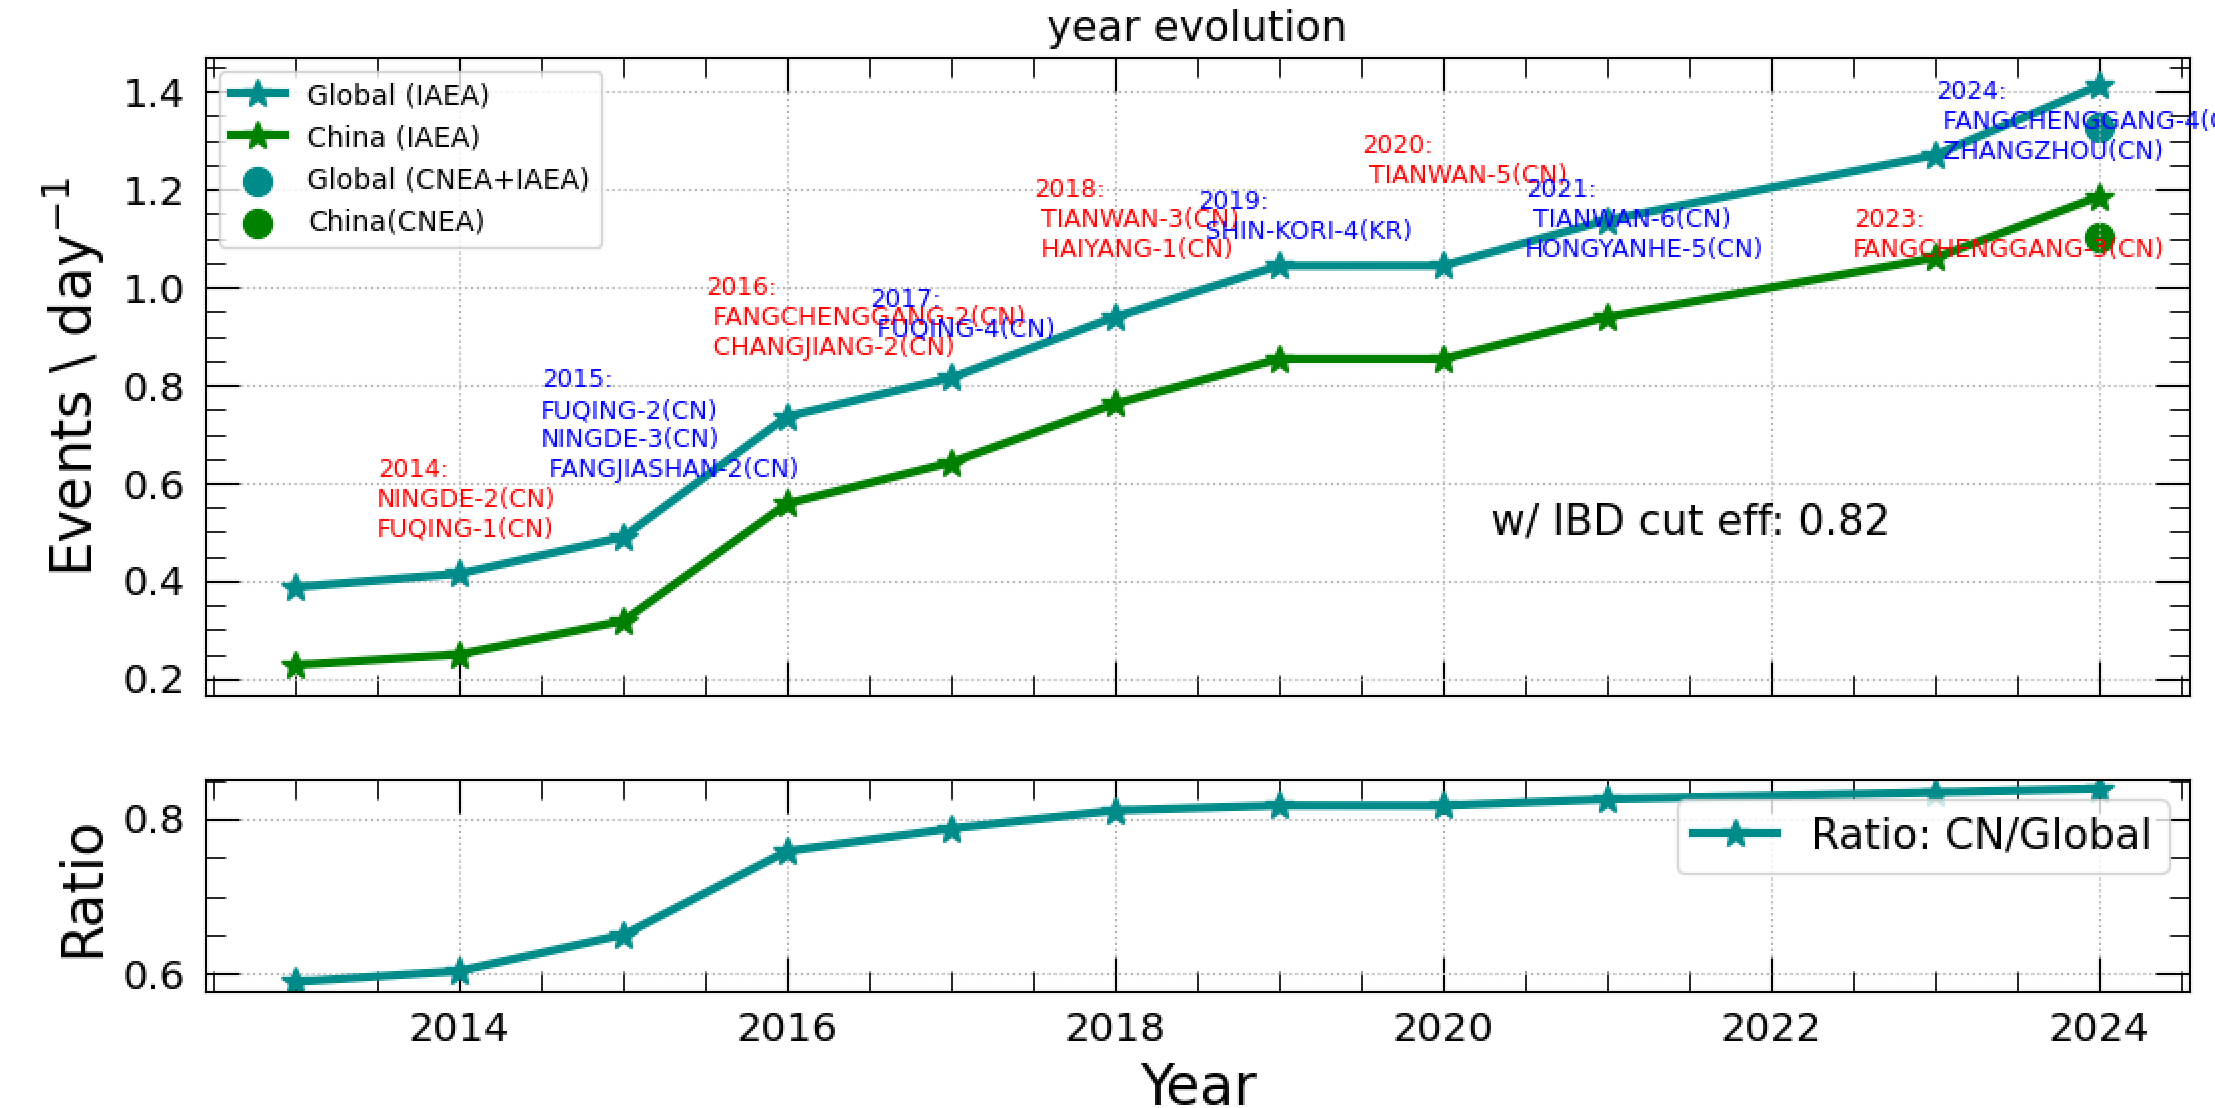
\includegraphics[width=0.75\linewidth]
    {3_background/Time_evolution-1_update.png}
    \caption{The yearly time evolution of IBD events from world reactor neutrinos \textcolor{red}{(with an nominal efficiency of 82\%)}.}
    \label{fig:WR-time-1}
\end{figure}


% \begin{figure}[h]
%     \centering
%     \includegraphics[width=0.75\linewidth]
%     {3_background/Time-evolution-2_update.png}
%     \caption{The quarterly time evolution of IBD events from world reactor neutrinos \textcolor{red}{(with an nominal efficiency of 82\%)}.}
%     \label{fig:WR-time-2_1}
% \end{figure}

\begin{figure}
    \centering
    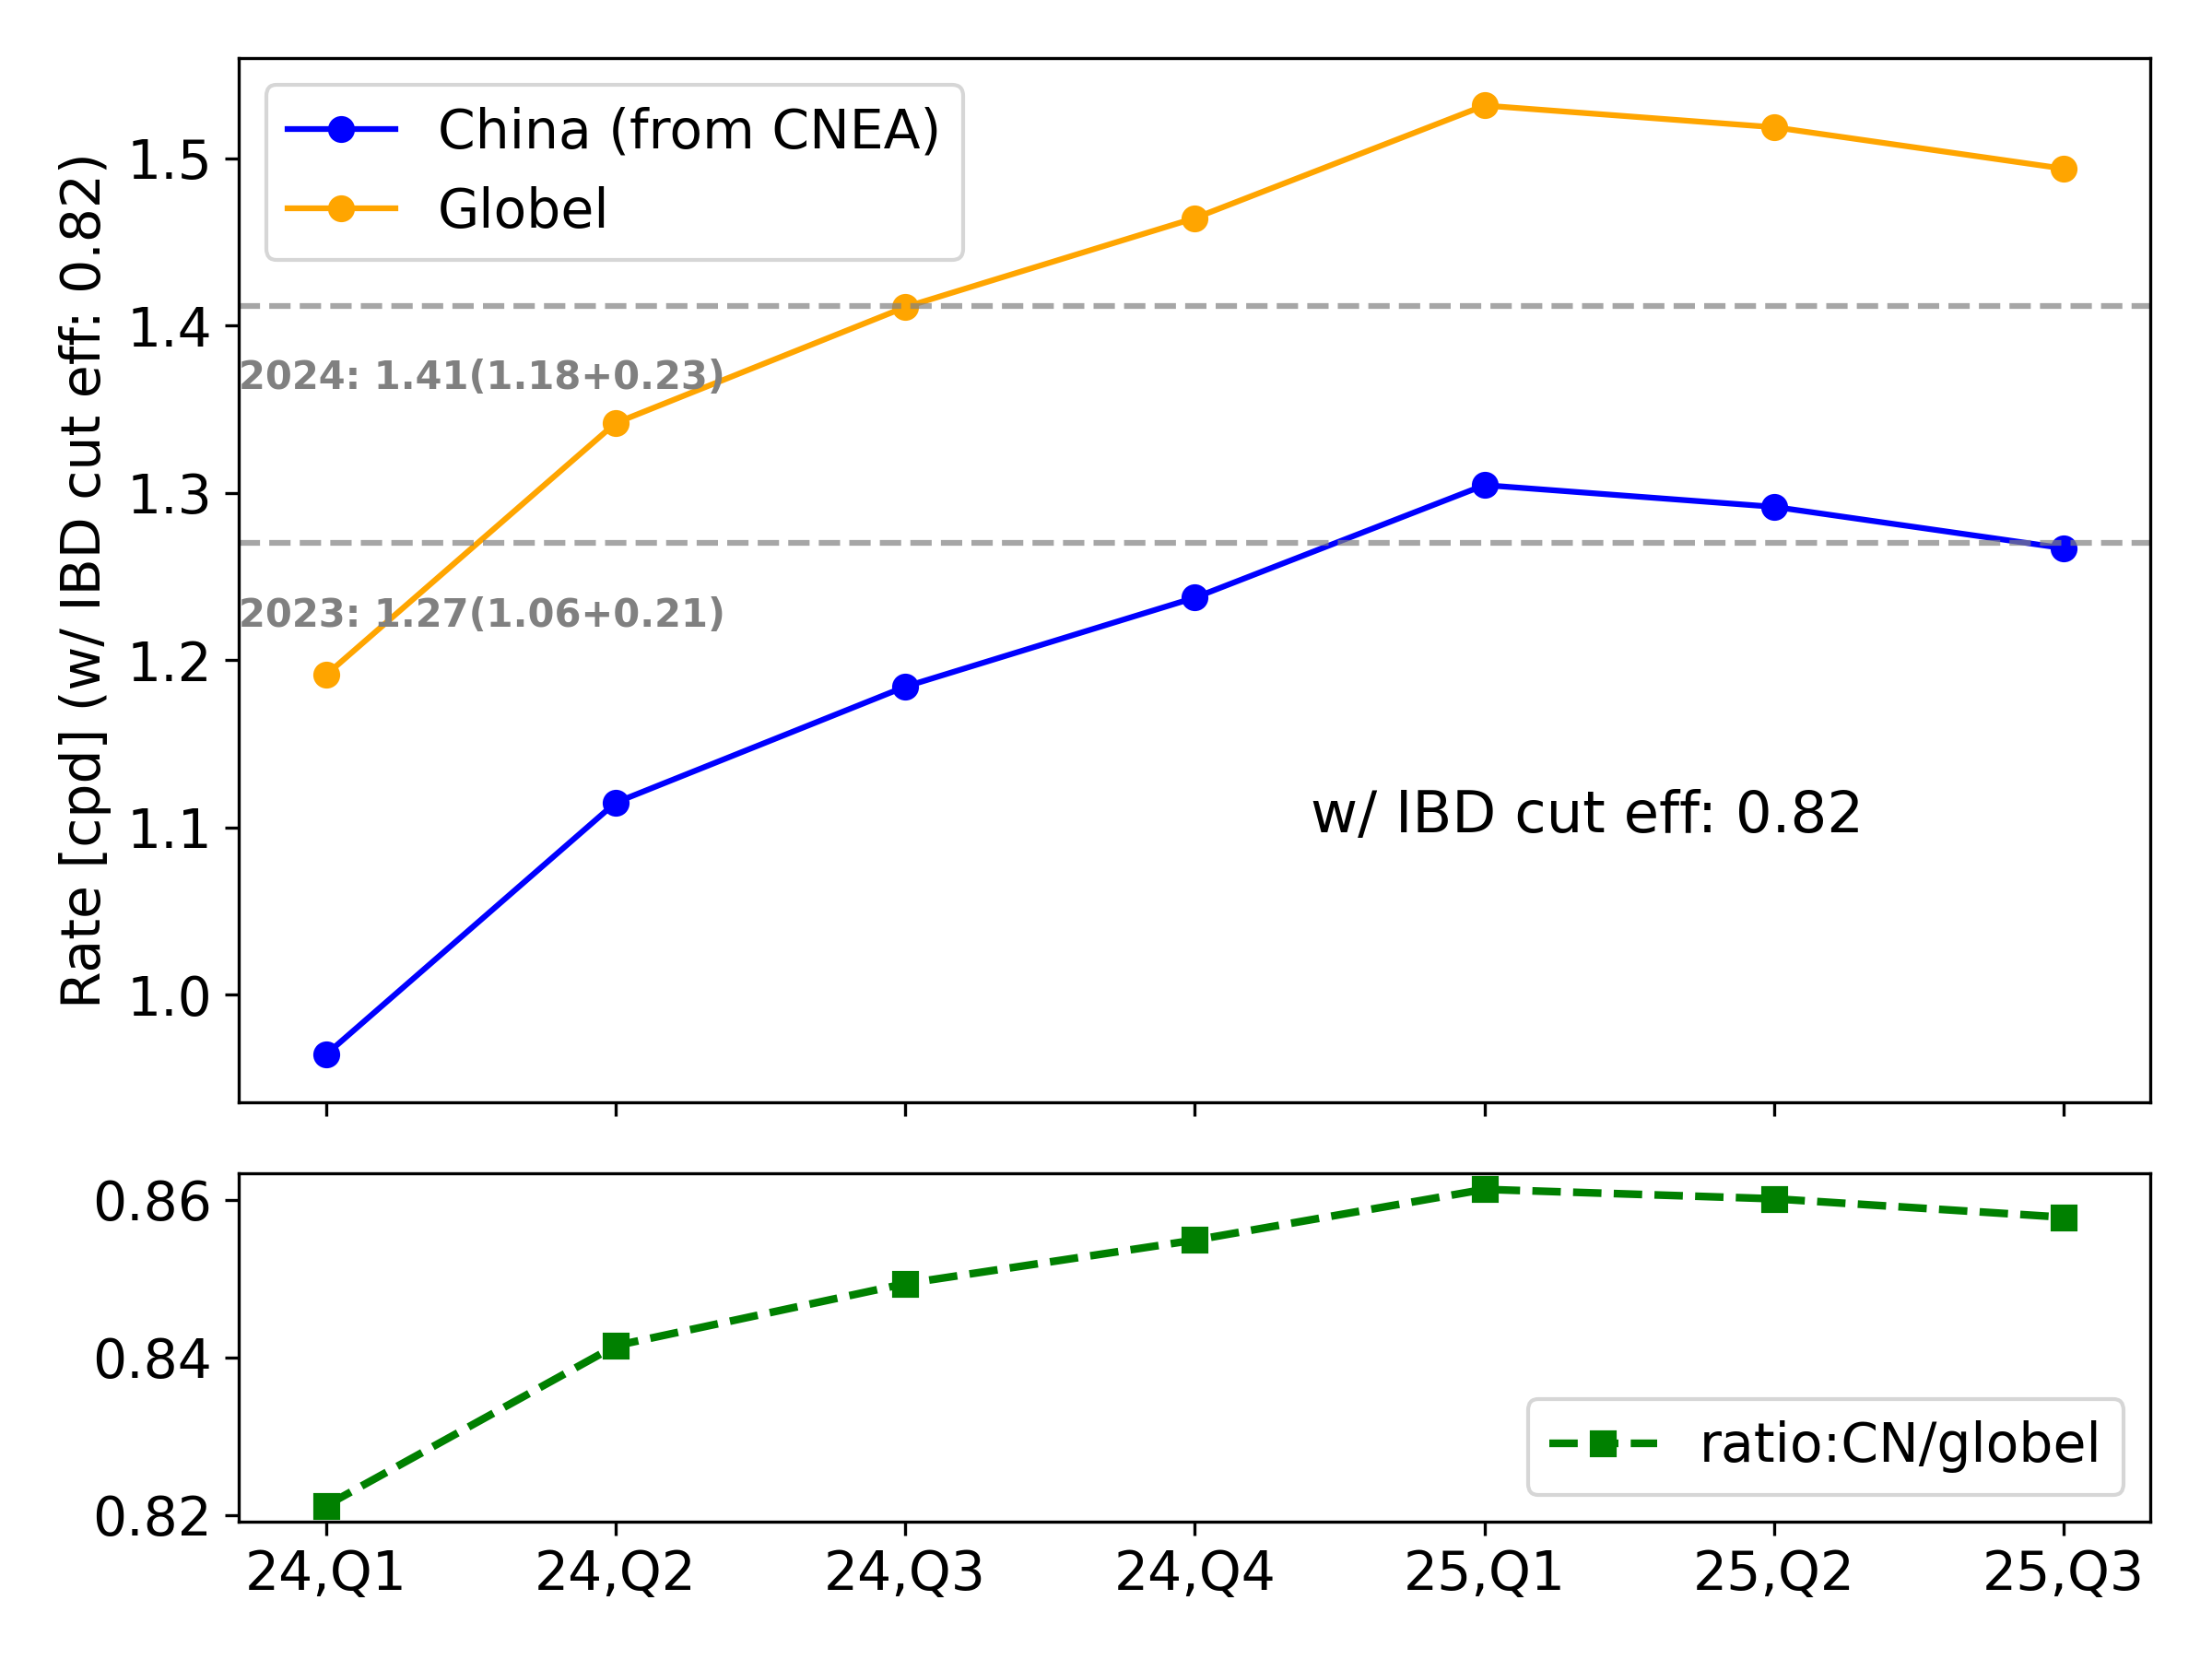
\includegraphics[width=0.75\linewidth]{3_background/time_evolution-3_update.png}
    \caption{The quarterly time evolution of IBD events from world reactor neutrinos \textcolor{red}{(with an nominal efficiency of 82\%)}.}
    \label{fig:WR-time-2}
\end{figure}




\begin{figure}[h]
    \centering
    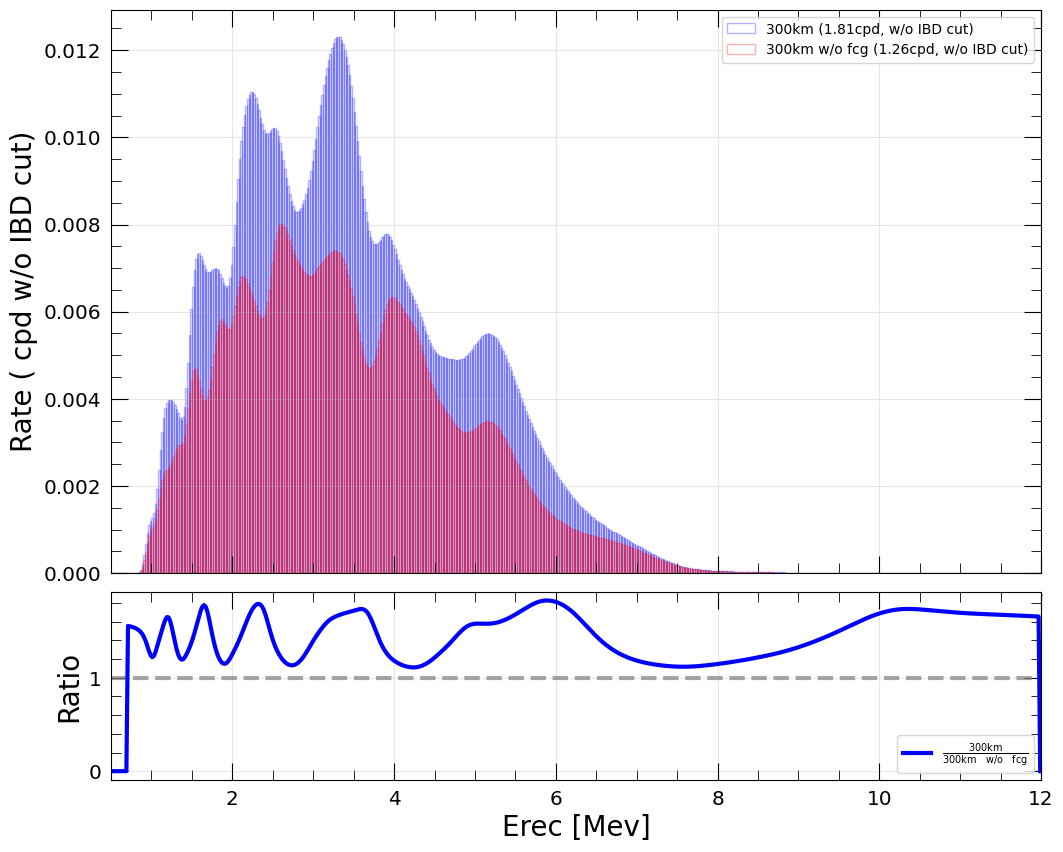
\includegraphics[width=0.7\linewidth]
    {3_background/time_evolution_update_251211}
    \caption{The spectrum shape of the IBD events from world reactor neutrinos. The detector response including energy resolution has been used.}
    \label{fig:WR-shape}
\end{figure}



From the time evolution study, we can conclude that contributions from reactors outside of mainland China are rather stable and the information in 2024 should be accurate enough for the current study. one the other hand, the reactor information for nearby reactors inside China should be as latest as possible. From Fig.~\ref{fig:WR-time-2}, we can observe that the first half year of 2025 is rather stable, and we are waiting for the third quarter release. 
Finally the reactors from Taiwan, China are absence from either of the above sources, thus we assume a distance of 1000 km and an effective thermal power of 10 ${\rm GW}_{\rm th}$.

We also calculate the neutrino events from research reactors from IAEA, and obtain the rate of $1.5\times10^{-3}$ cpd, which can be negligible.

By taking the duty factor information for the second quarter of 2025 in CNEA and all the others for the average one of 2024 in IAEA, we can calculate the event rate of world reactor neutrinos as 1.48 cpd \textcolor{red}{with an nominal efficiency of 82\%}. The spectrum shape of the world reactor neutrinos is shown in Fig.~\ref{fig:WR-shape}, and the detector response including energy resolution has been used. From the figure one can observe that the oscillation effect is still significant.

For the uncertainty evaluation, we mostly follow the method for the signal part, but the exception is the fission fraction is not known and one can only rely on the typical burnup period to make an educated guess. Since the fission fraction range of $^{235}{\rm U}$ could vary from 75\% to 50\%, we emply a half range of around 12\% to evaluate its induced uncertainty (see DocDB: 13065).
For Scenario A, by combining the uncertainty of thermal power (0.5\%), fission fraction (1.1\%), IBD yield (2\%) and detection (1.8\%) induced uncertainties, \textcolor{red}{we can have the total rate uncertainty of 3\%. Finally, considering the time delay of available reactor information, we would like to enlarge the rate uncertainty to 10\%}. The shape uncertainty is mainly from isotopic spectra from four isotopes. \textcolor{red}{It is evaluated as 5\%} from the theoretical model consideration (see DocDB: 5929), thus will keep unchanged for different binning scheme.
An alternative evaluation using the data driven method (from DYB data) will be provided soon.

Finally we want to comment that the oscillation effect is fixed when the world reactor neutrinos are considered as the background.
This may induce bias for the oscillation parameters when the true parameters are different from the current PDG central values. 
A study by comparing the world reactor neutrinos as either the signal (oscillation is properly considered for all reactors) or the background of Scenario A (the oscillated spectrum is fixed at the PDG central value) is employed and illustrated in Fig~\ref{fig:WR-bias}. The bias is around $0.05\sigma$ for 50 days of data, and will increase to $0.2\sigma$ for 6 years.
\begin{figure}[h]
    \centering
    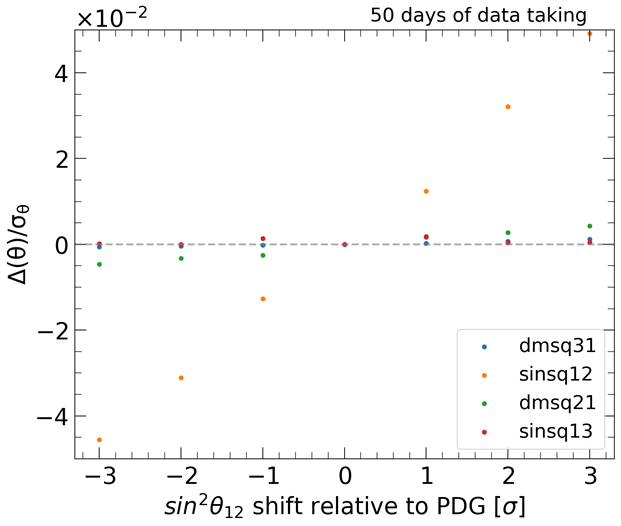
\includegraphics[width=0.7\linewidth]
    {3_background/WR-Bias-theta12.png}
    \caption{The induced bias of oscillation parameters by treating the world reactor neutrinos of further than 300 km (Scenario A) as fixed background, and assuming a shift of $\sin^2\theta_{12}$ relative the PDG value (bias induced by the shift of other parameters is smaller). The data taking time is 50 days.}
    \label{fig:WR-bias}
\end{figure}

\textcolor{red}{Given that the signal contribution from the Fangchenggang reactor accounts for a significant proportion of the overall signal from world reactors, and detailed operational information about this reactor is accessible, in our first paper, we incorporate Fangchenggang as a signal reactor (building upon the existing set of signal reactors), while classifying other reactors located more than 300 km away as world reactors and the uncertainty is same with before.}
%Our plan for this analysis of 50 days data is to employ Scenario B, because it can both largely reduce the bias and take into account the availability of reactor information.
%A quantitative test for this option will be provided soon.


\subsection{Geo-neutrinos}
%By Rongping.

%Geo-neutrinos are produced 
Geo-neutrinos are generated from the beta decay chains of the nuclear isotopes with long half-lives such as $\Um$, $\Th$, and $\K$ inside the Earth. At the JUNO detector, only the geo-neutrinos from $\Um$ and $\Th$ are observable above the threshold energy of the inverse beta decay (IBD) reaction ($\bar{\nu}_e + p \to e^+ + n$).

To make the prediction for the geo-neutrino singal, we make a new assessment of individual geo-neutrino fluxes by using the summation method from the decay chains of $\Um$ and $\Th$. The integration of the updated nuclear database, consideration of forbidden transitions, and inclusion of higher-order corrections yield significant spectral deviation compared to the currently commonly used Enomoto fluxes.
Compared to the Enomoto flux model, the IBD yield will have a decrease of $3.47\%$ for $\Um$ and $9\%$ for $\Th$.
Meanwhile, the spectral comparison is shown in Fig.~\ref{fig:geoUTh}. The spikes come from small changes of the Q values of beta branches, and the shape distortion is due to the forbidden decay features. The spectra used in the fitting will be convoluted with the IBD interaction with neutron recoils, the detector response and resolution.
\begin{figure}[h]
    \centering
    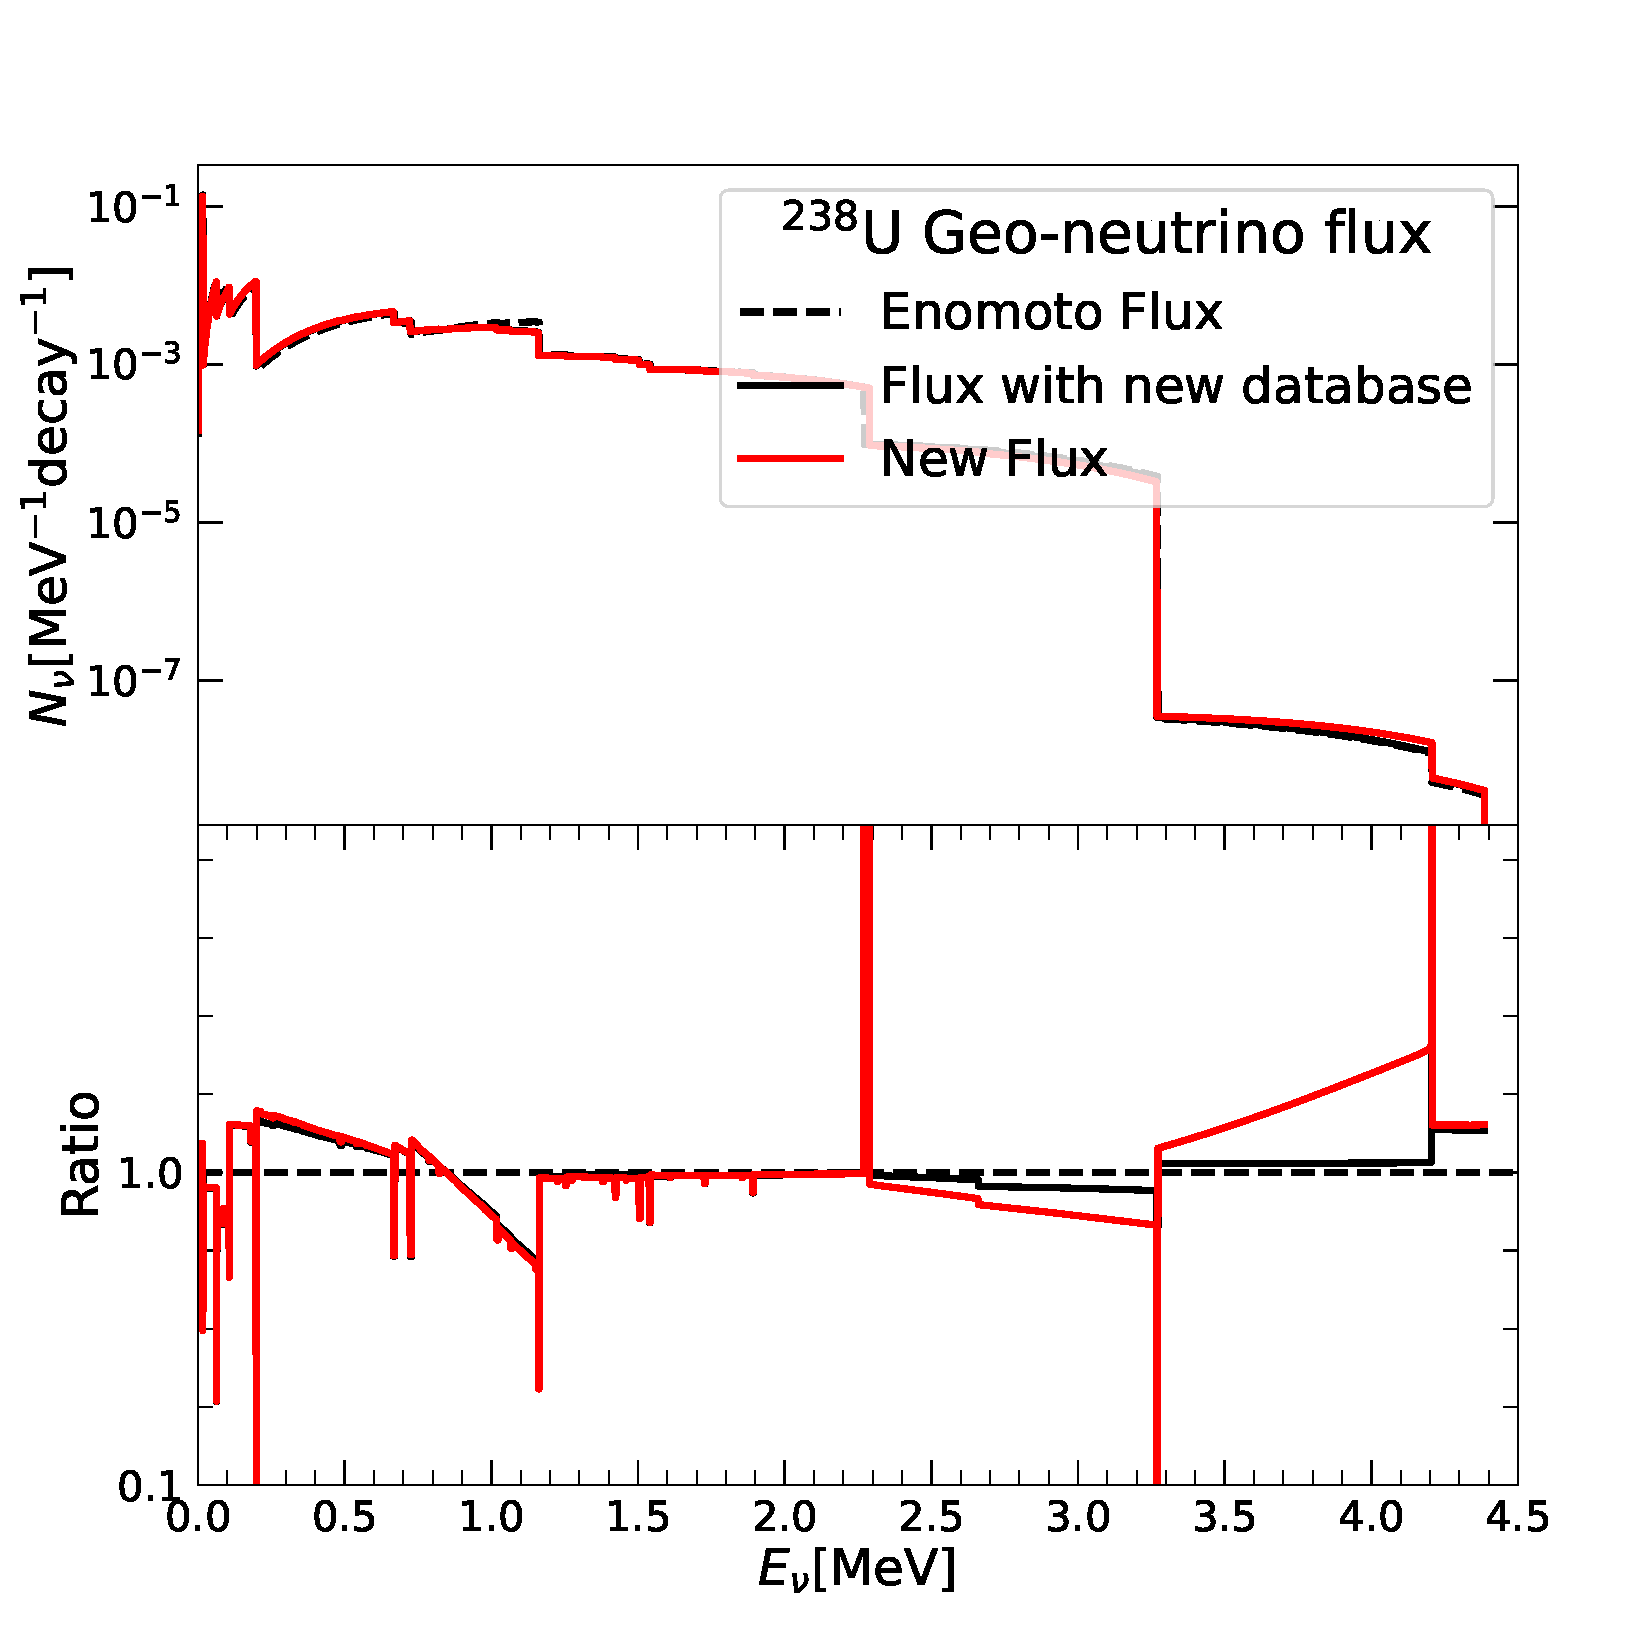
\includegraphics[width=8cm]{3_background/geoU238.pdf}
    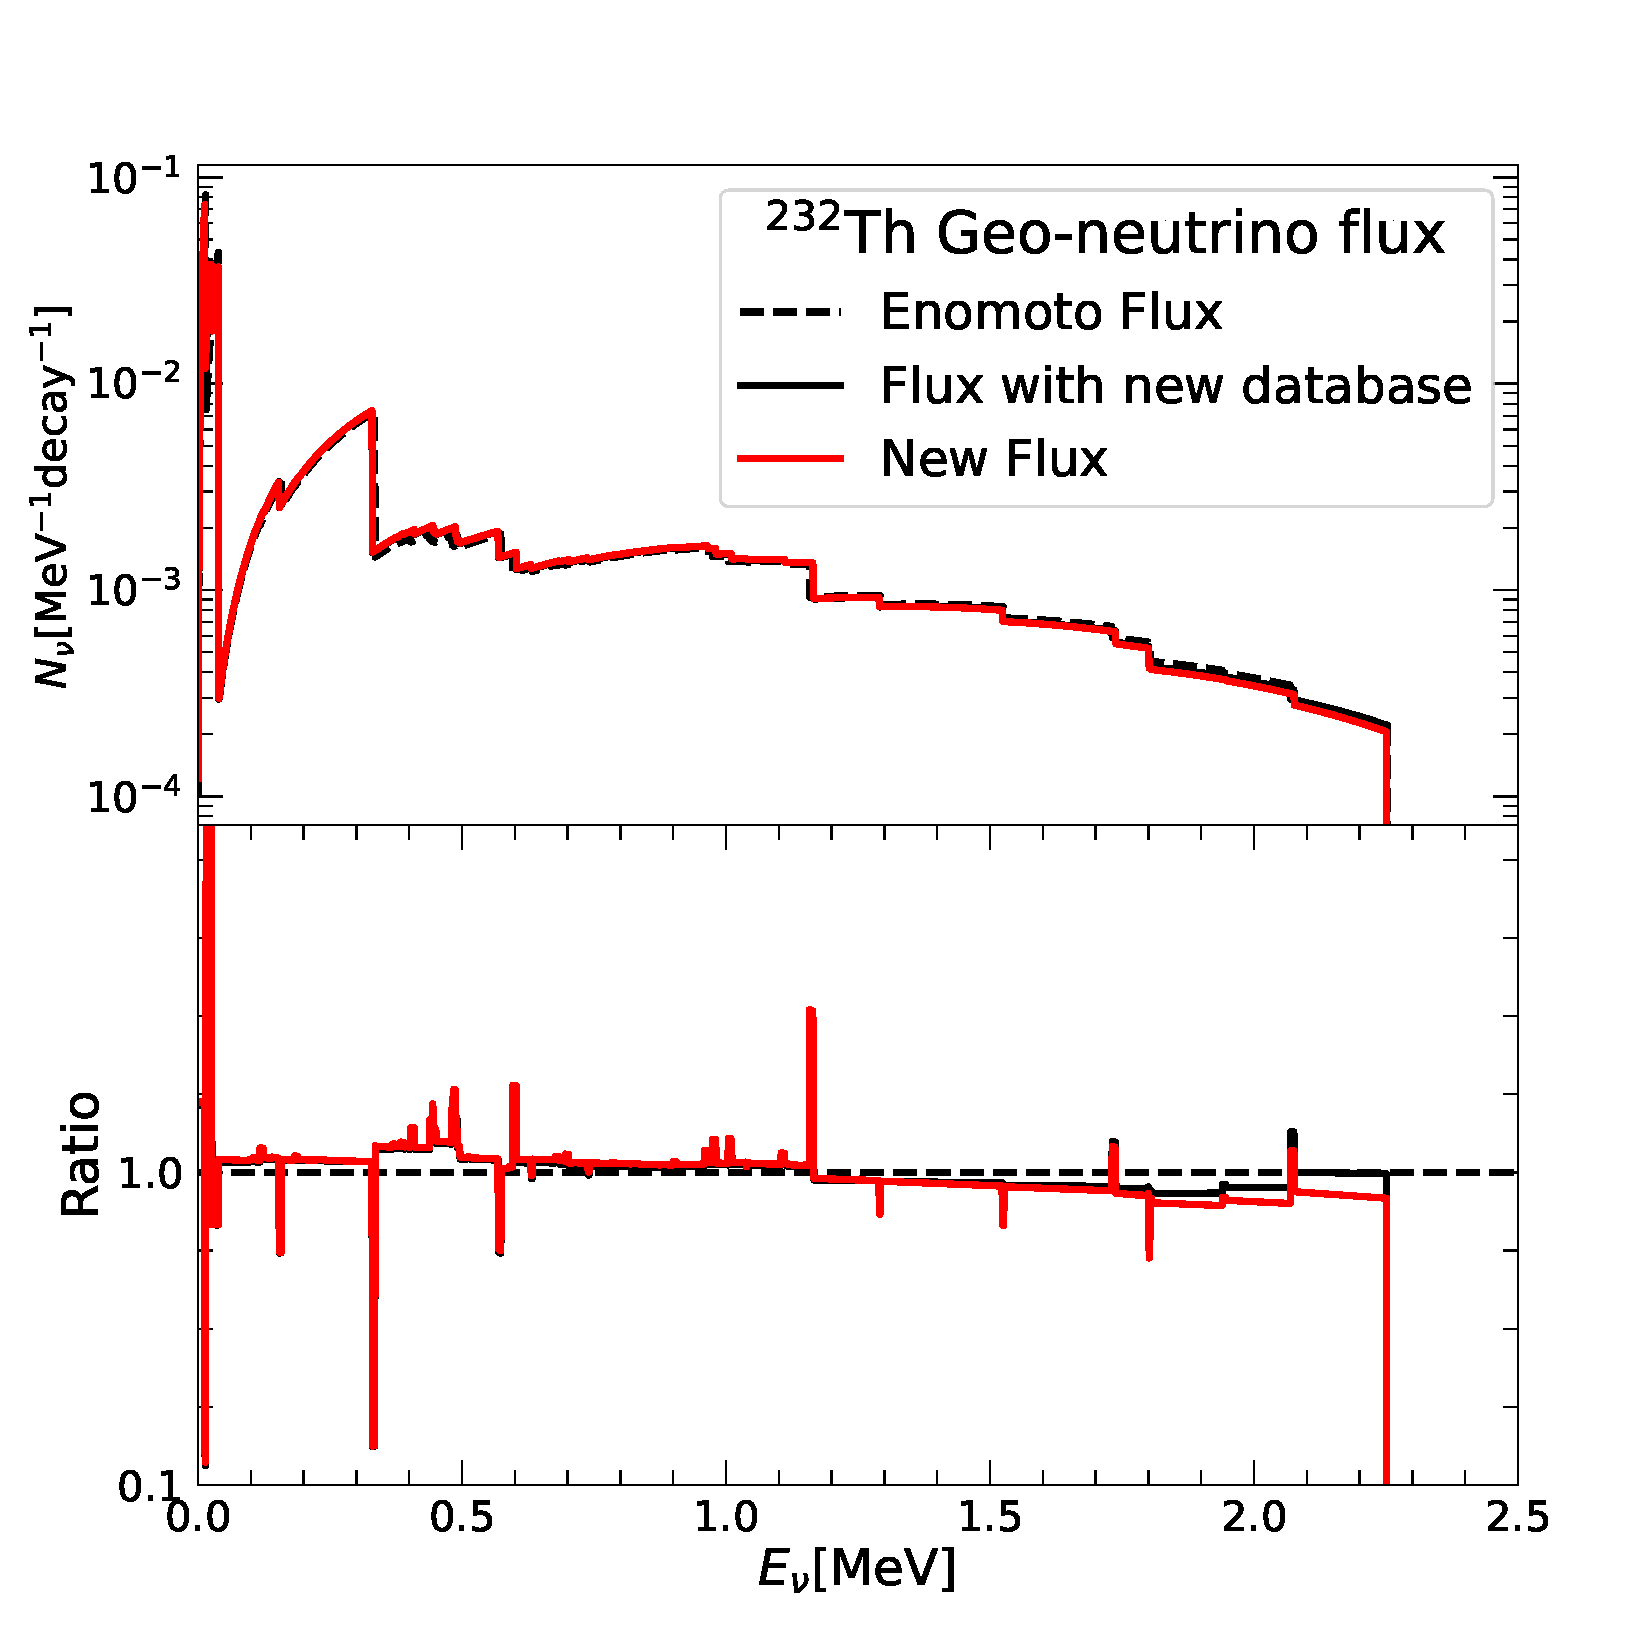
\includegraphics[width=8cm]{3_background/geoTh232.pdf}
    \caption{The geo-neutrino energy spectra from the decay chains of $\Um$ and $\Th$.}
    \label{fig:geoUTh}
\end{figure}

The rate of geo-neutrino signals depends on the inputs of geo-science information [see DocDB:13109, and tech-note and paper draft of geo-neutrino sensitivity paper DocDB: 14784]. For the crustal contribution, most of the variations are from either using the abundance of local rock samples near the JUNO site or the average values, in which the crust rates are ranged from $30.9^{+6.5}_{-5.2}$ TNU of the RRM model, to $40.4^{+5.6}_{-5.0}$ TNU of the JULOC model. For the mantle contribution, the variation are even larger, with three categories of poor-H, medium-H and rich-H models, having the rates of $\sim 2.8$ TNU, $\sim8.0$ TNU, and $\sim17.4$ TNU respectively. By directly combining the whole range of crustal and mantle contributions, the geo-neutrino rate can range from 27.5 TNU to 63.4 TNU. In order to cover the whole range and to be model independent, we choose the value  $44.3\pm18$ TNU [$1.75(1\pm40\%$) cpd](100\% efficiency). Note that totally free or 100\% uncertainty is an alternative choice.

% we choose the central value and half range as the rate uncertainty consideration, i.e., $45.5\pm18$ TNU [$1.4(1\pm40\%$) cpd]. Note that totally free or 100\% uncertainty is an alternative choice.

Typically we can choose a $\sim 5\%$ shape uncertainty for the database and beta decay uncertainty. The uncertainty from oscillation parameters is evaluated to be at the percentage level and can be included in the $5\%$ shape uncertainty. Note that the sensitivity of all parameters has negligible change when the shape uncertainty is increased to 20\% . 

\textcolor{red}{In our first paper, we also placed constraints on the U/Th ratio of the geoneutrino background, with an associated uncertainty of 10$\%$,and the center value of the ratio is 0.29.}

\subsection{Atmospheric neutrinos}
Atmospheric neutrino neutral current interaction with the carbon nuclei can knock out nucleons and introduce correlated IBD backgrounds. The event rate relative for reactor IBD analysis from such events were studied comprehensively in \cite{nc_epjc_2024}. Using state-of-the-art neutrino interaction models including GENIE (3.0.6) and NuWro (19.02), the impact on the event rate in the IBD energy region [0.7, 12] MeV due to nuclear models, final state interactions are studied. Using the avearge of five selected representing models, the nominal NC background rate is calculated to be 2.1$\pm$0.7 kton$^{-1}$yr$^{-1}$ (or 0.12$\pm$0.04 cpd in 20kton LS). The de-excitation of final state particles is implemented with a TALYS-based model. A 10\% rate difference is observed with de-excitation effect turned on and off. Therefore, a conservative 10\% rate error is assigned for de-excitation. Taking into another 10\% rate uncertainty from atmospheric neutrino flux, a total 50\% rate error is quoted.

The shape error is accounted by the shape-only distortion of each model w.r.t. the average model as 1$\sigma$ deviation \cite{nc_nominal}. Therefore, the NC background spectrum is treated in the following way:

\begin{equation}
    f(E) = A(f_0(E) + \sum_{i=1}^{5}a_if_i(E) )
\end{equation}

where $f_0(E)$ is the nominal model, $f_i(E)$ is the shape-only difference between the $i$-th model and the nominal model. $A$ is the rate nuisance parameter contrained to follow Gaus(1, 0.5) and $a_i$ follows Gaus(0, 1).

\subsection{Summary}
\begin{table}[!htbp]
    \caption{Summary of signal and backgrounds. The detection efficiencies are included. }
    \centering
    \footnotesize% fontsize
    \setlength{\tabcolsep}{4pt}% column separation
    \renewcommand{\arraystretch}{1.2}%row space
    %\resizebox{\linewidth}{!}{
    \begin{tabular}{lcc}
        \hline
          & Selection A1 & Shape uncertainty \\ 
        \hline
        $\overline{\nu}_{e}$ candidates & 2379 & - \\
        DAQ live time (days) & 59.08 & - \\
        Geoneutrinos (day$^{-1}$) & 1.23$\pm$0.49 & 5\% bin-to-bin + Th/U=0.29$\pm$0.03\\
        World reactors (day$^{-1}$) & 0.88$\pm$0.09 & 5\% bin-to-bin \\
        Accidentals (day$^{-1}$) & 0.049$\pm$0.003 & 20\% \\
        BiPo214 (day$^{-1}$) & 0.18$\pm$0.10  & 5\% \\
        Fast neutron (day$^{-1}$) & 0.02$\pm$0.02 & 60\% \\
        Double neutron (day$^{-1}$) & 0.05$\pm$0.05 & 50\% \\
        \Li~(day$^{-1}$) & 4.28$\pm$1.44 & 20\% \\
        %B12-B12 & <0.02 & xx \\
        Atmospheric neutrinos (day$^{-1}$) & 0.08$\pm$0.04 & Option2 in DocDB-14940 \\
        $^{13}$C ($\alpha, n$) $^{16}$O (day$^{-1}$) & 0.04$\pm$0.02  & 50\% bin-to-bin \\
        %$\overline{\nu}_{e}$ rate  (day$^{-1}$) & xx$\pm$xx & -\\
        \hline
    \end{tabular}
    %}
    \label{tab:selResults}
\end{table}



\section{Efficiency calculation and systematic uncertainty analysis}

\subsection{Detection efficiency}
The predicted IBD number is calculated as
\begin{equation}
    N_{IBD} = \phi_{\nu}\sigma_{\rm IBD}N_{p} \epsilon_{\mu}\epsilon_{m}\epsilon_{\rm FV}\epsilon_{ep}\epsilon_{ed}\epsilon_{dt}\epsilon_{dr}
    \label{eq:pred_ibd_num}
\end{equation}
where $\phi_{\nu}$ is the reactor neutrino flux, $\sigma_{\rm IBD}$ the IBD reaction cross section, $N_{p}$ the number of target proton and $\epsilon_{i}$ the detection efficiency for the i-th cut.

In this section, we present the estimation of all the detection efficiencies and their corresponding systematic uncertainties.


\subsubsection{Target proton number}
We take the results from DocDB-14944.
The target proton number is estimated as $1.442 \times 10^{33}$ with the relative uncertainty 1\%.

\subsubsection{Fiducial volume cut}
In principle, the efficiency of FV cut can be calculated analytically. In this geometric calculation, we assume a perfect sphere, and the efficiency can be calculated as 
\begin{equation}
    \epsilon_{\rm FV} = \left(\frac{R_{\rm FV}}{R_{\rm CD}}\right)^{3} = 81.01\%
    \label{eq:fv_eff}
\end{equation}
Including the efficiency of z cut, the final effiency is 80.57\%.
Considering the bias of vertex reconstruction of 10 cm [DocDB-14862], it leads to $\sim$ 1.8\% uncertainty of the efficiency.

To do a data-driven estimation of the efficiency, spatially homogeneous samples are needed.
There are three alternative samples for the estimation: B12, SPN tagged Li9 and high-energy IBDs.
Moreover, the systematic uncertainty can be constrained by comparing the analysis using these three kinds of samples as well.

For B12 events, MC studies reveal that B12 events produced by muons with deposited energy > 0.5 GeV have nearly uniform radial vertex distribution (with the contribution from muons with energy < 0.5 GeV being negligible), as shown in Fig. \ref{fig:B12_r3_mc}.
This conclusion is confirmed with data, as shown in Fig. \ref{fig:B12_r3_data}.
Significant edge effect is found in data, which needs more careful investigation.

\begin{figure}[h]
  \centering
  \begin{subfigure}[t]{0.52\textwidth}
    \centering
    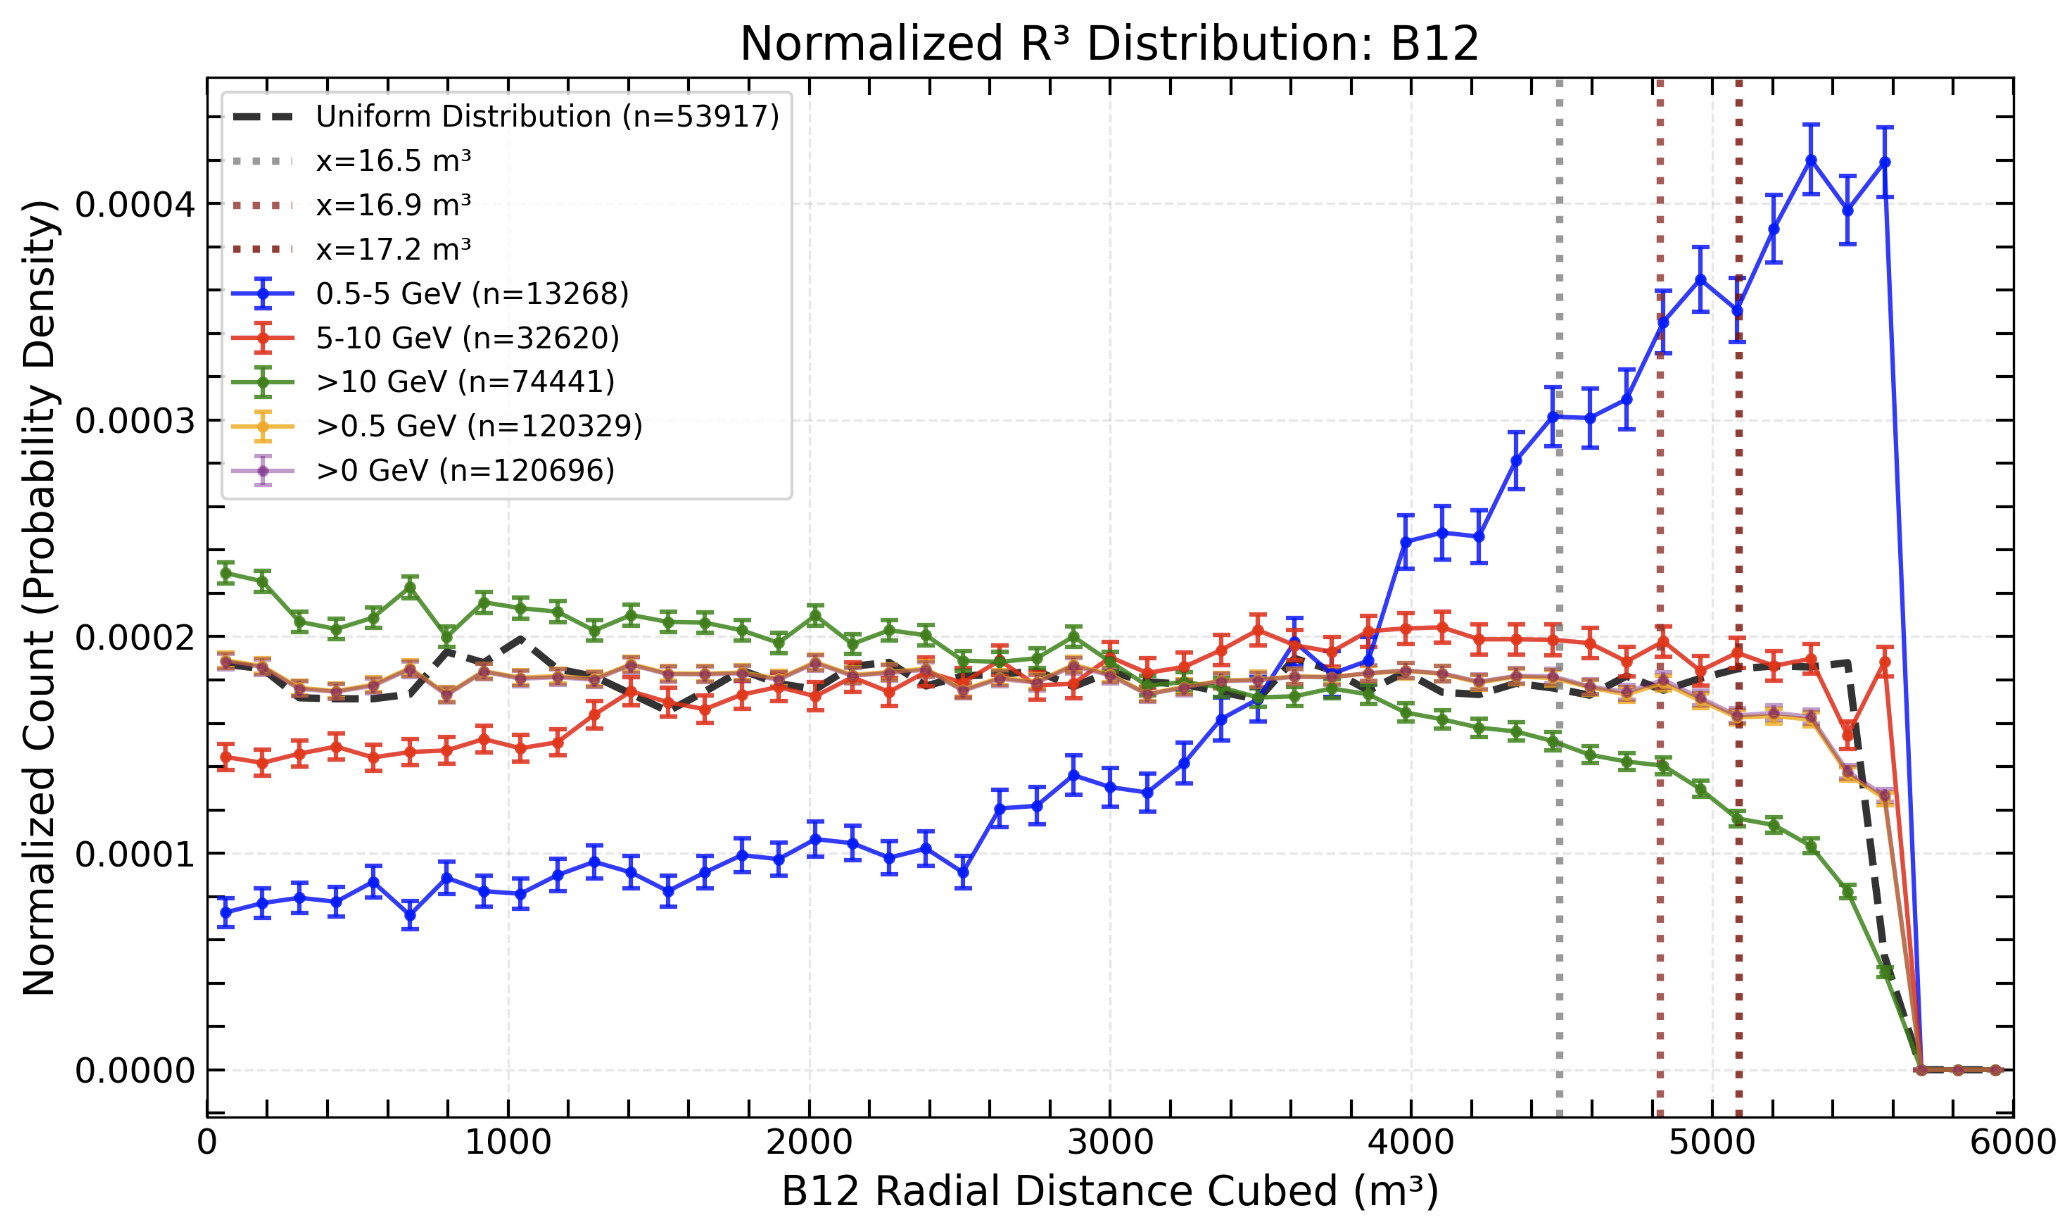
\includegraphics[width=\linewidth]{4_efficiency/B12_r3_mc.png}
    \caption{}
    \label{fig:B12_r3_mc}
  \end{subfigure}
  \hfill
  \begin{subfigure}[t]{0.43\textwidth}
    \centering
    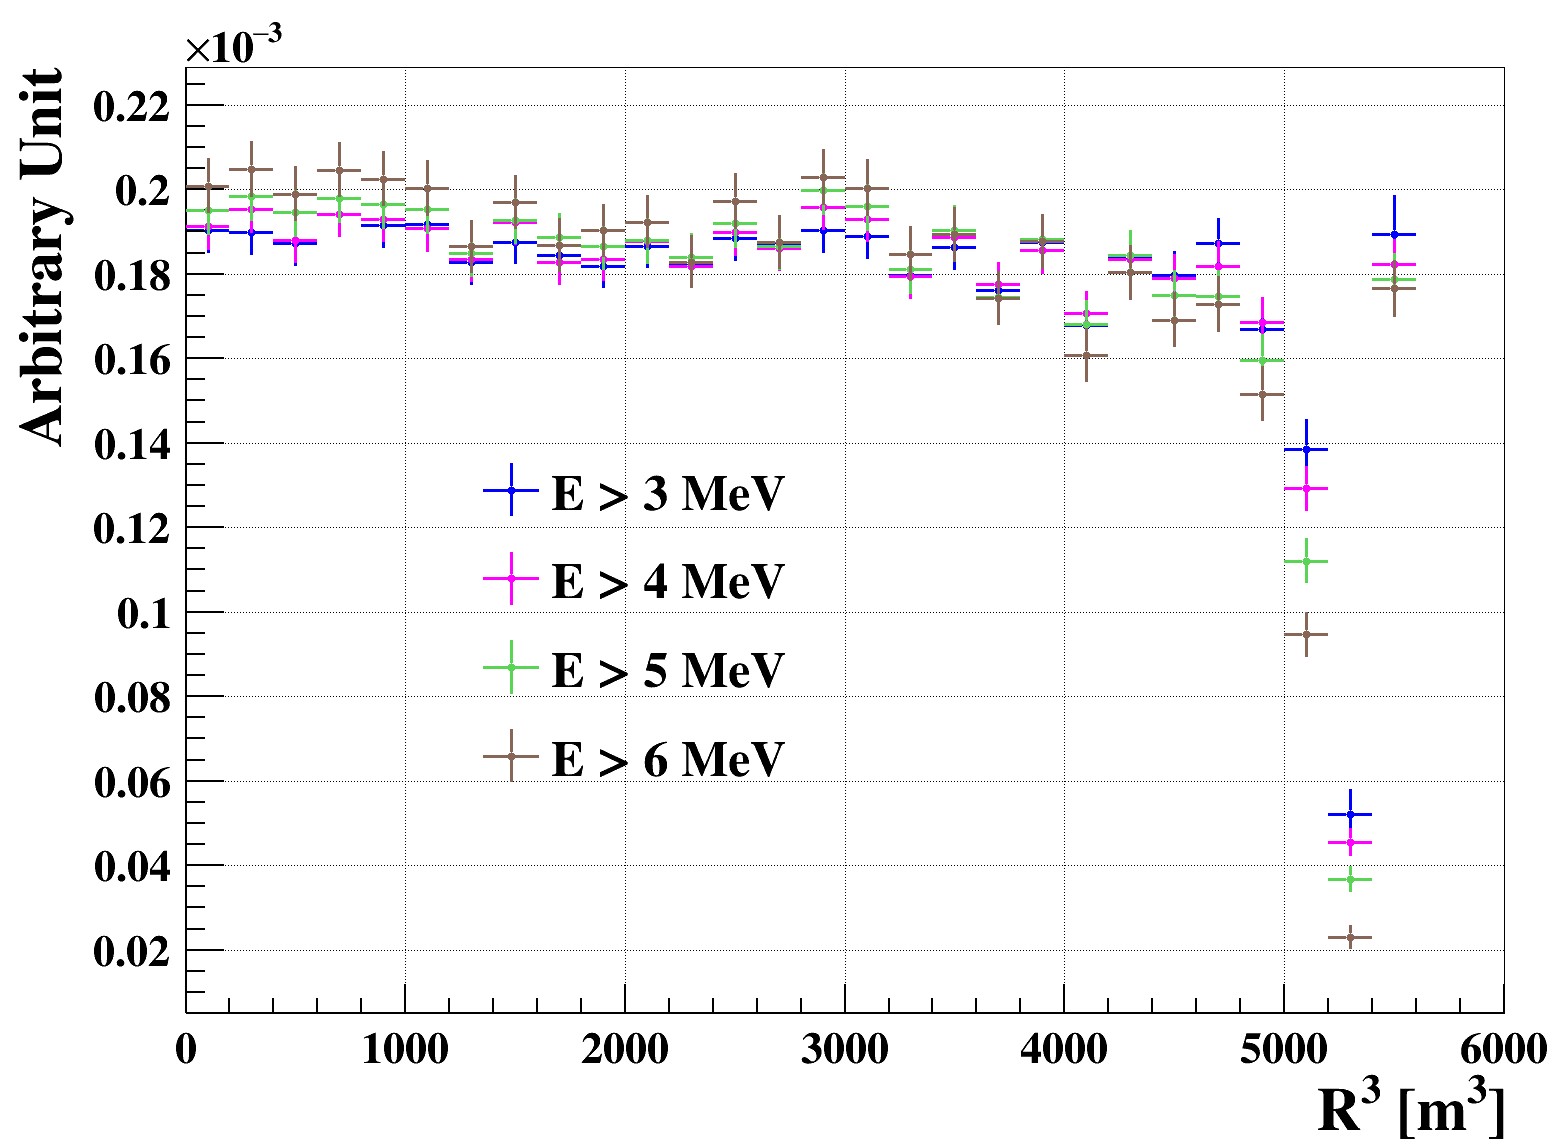
\includegraphics[width=\linewidth]{4_efficiency/B12_r3_data.png}
    \caption{}
    \label{fig:B12_r3_data}
  \end{subfigure}
  \caption{Radial vertex distribution of B12 in (a) MC and (b) data tagged by muons with reconstructed energy > 0.5 GeV.}
\end{figure}

As shown in Fig. \ref{fig:li9_r3_mc}, Li9 events produced by muons with deposited energy > 0.5 GeV have nearly uniform radial vertex distribution as well, which can be selected with neutron tagging in data.

\begin{figure}
    \centering
    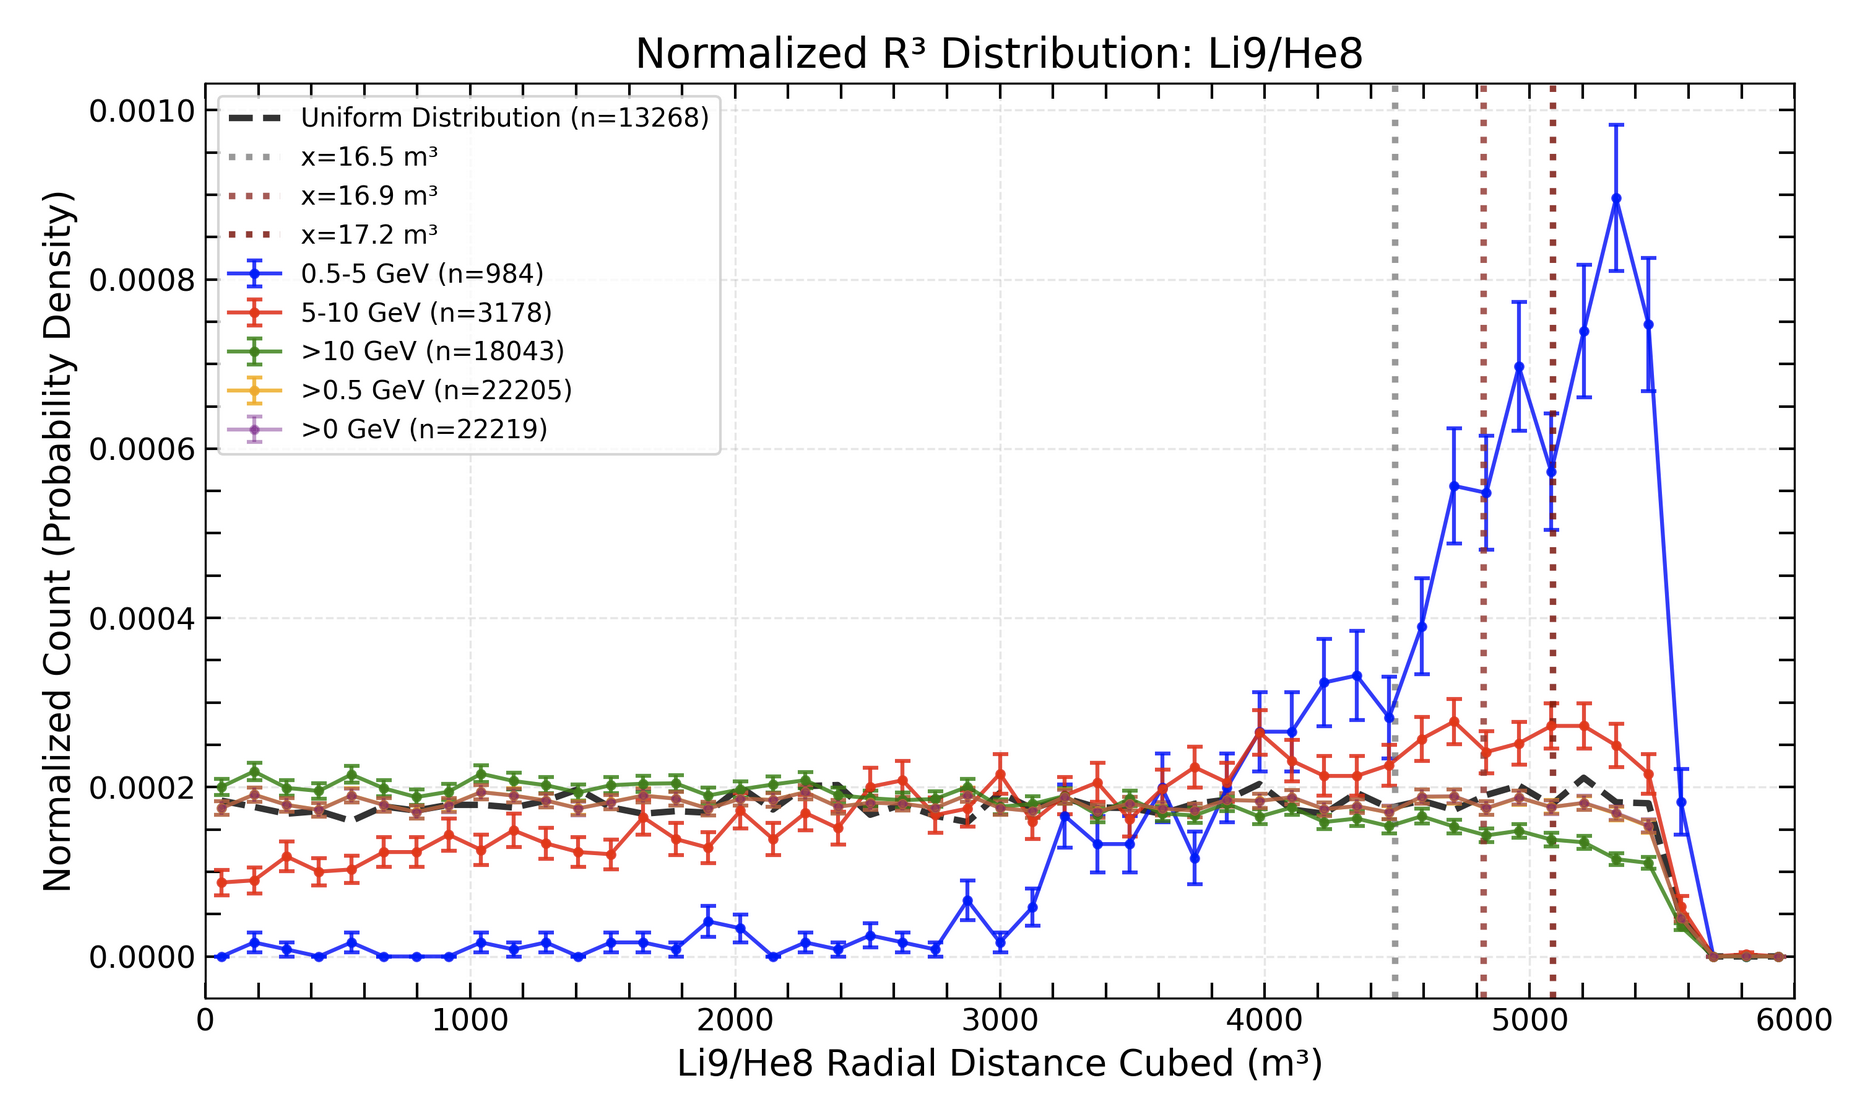
\includegraphics[width=0.5\linewidth]{4_efficiency/li9_r3_mc_v2.png}
    \caption{Radial vertex distribution of Li9 in MC.}
    \label{fig:li9_r3_mc}
\end{figure}

The efficiency also can be estimated with high-energy IBD samples, which is a more reasonable way [DocDB-15101].
To study the efficiency, FV cut is removed and high-energy cut is applied.
As shown in Fig. \ref{fig:IBD_candidate_spectra_fvCut}, after the cut ($E_p$ > 3.5 MeV), the accidental background should be negligible.
Additionally, SPN veto is removed to include more statistics and ensure uniform vertex distribution.
Fig. \ref{fig:IBD_r3_ed_beforeSPN} shows the $r^3$-vertex distribution after all above cuts, indicating nearly uniform radial distribution.


\begin{figure}[h]
  \centering
  \begin{subfigure}[t]{0.45\textwidth}
    \centering
    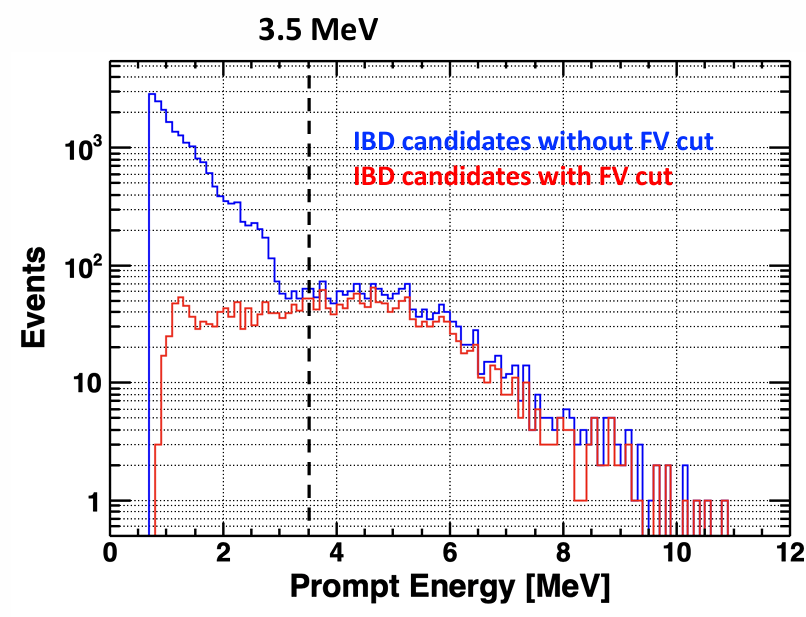
\includegraphics[width=\linewidth]{4_efficiency/IBD_candidate_spectra_fvCut.png}
    \caption{}
    \label{fig:IBD_candidate_spectra_fvCut}
  \end{subfigure}
  \hfill
  \begin{subfigure}[t]{0.5\textwidth}
    \centering
    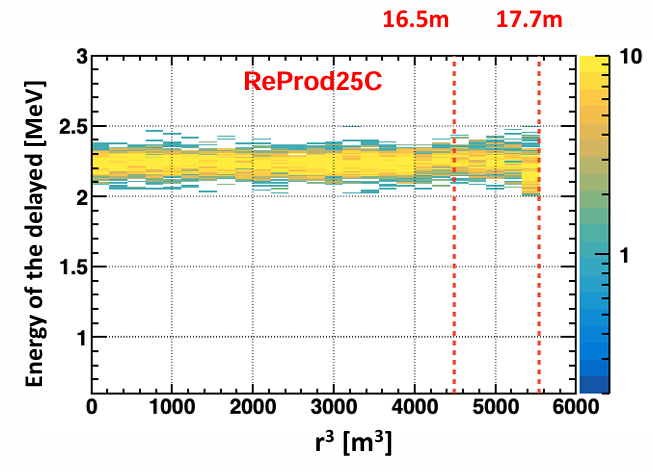
\includegraphics[width=\linewidth]{4_efficiency/IBD_r3_ed_beforeSPN.png}
    \caption{}
    \label{fig:IBD_r3_ed_beforeSPN}
  \end{subfigure}
  \caption{(a) Prompt spectra of IBD candidates without (blue line) and with (red line) FV cut. (b) $r^3$-$E_d$ distribution  of IBD candidate with prompt energy > 3.5 MeV and without FV cut and SPN veto.}
\end{figure}

Subsequently, the FV cut efficiency could be estimated as
\begin{equation}
    \epsilon^{\rm IBD}_{\rm FV} = \frac{\text{(IBDs with FV cut)}}{\text{(IBDs without FV cut)} \times (1+\epsilon_{\text{spill-out}})} (E_p > 3.5 \text{MeV})
    \label{eq:fv_eff_ibd}
\end{equation}
where $\epsilon_{\text{spill-out}}$ is the correction factor by spill-out effect where IBD neutrons could leak out LS region near the CD edge. Using 10 keV neutron MC samples provided by Peidong Yu, $\epsilon_{\text{spill-out}}$ is estimated as 2.4\%.
Then, the efficiency is calculated as ($79.61 \pm 0.58 (\text{stat.})$)\%.
The relative difference between geometric calculation and the estimation based on high-energy IBD sample is 1.2\%, which is consistent with each other.

The uncertainty could be estimated by the variation of the number density of IBD candidates near the FV edge.
As shown in Fig. \ref{fig:IBD_r3_density_omilrec}, the average density in FV is calculated as $d_{\text{inFV}}$ = 0.186 events/m$^3$, and the density in $r=[16, 16.5]$ m regions is $d_{r=[16, 16.5] m}$ =  0.15 events/m$^3$.
Then the uncertainty is estimated as 
\begin{equation}
    \sigma_{\rm FV} = 1 - \frac{V(r<16m) \times d_{\text{inFV}} + V(16<r<16.5m) \times d_{r=[16, 16.5] m}}{V(r<16.5m) \times d_{\text{inFV}}} = 1.6\%
    \label{eq:fv_eff_ibd}
\end{equation}

\begin{figure}
    \centering
    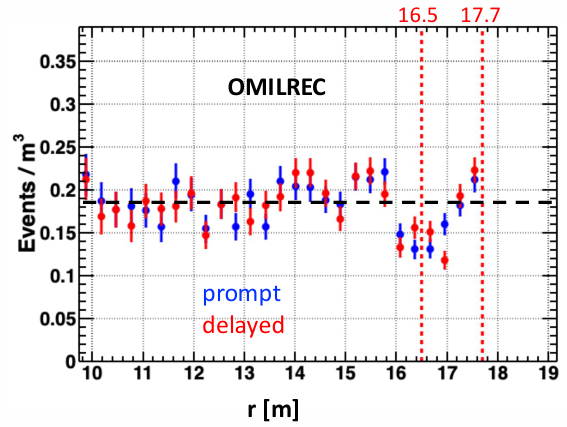
\includegraphics[width=0.5\linewidth]{4_efficiency/IBD_r3_density_omilrec.png}
    \caption{The number density of IBD candidates along radial direction. The black dashed line represents the average density in FV.}
    \label{fig:IBD_r3_density_omilrec}
\end{figure}


\subsubsection{Muon veto}
To suppress cosmogenic backgrounds, three types of muon veto strategies are designed:
\begin{itemize}
    \item WP and CD muon veto: apply on delayed signals over the whole target volume.
    \item Spallation neutron (SPN) veto: apply on delayed signals inside the sphere around spallation neutron events.
    \item Muon track veto (not included in this note): apply on delayed signals around muon tracks.
\end{itemize}

For the first type of muon veto, the corresponding efficiency is calculated as the ratio of live time to DAQ time:
\begin{equation}
    \epsilon_{\mu,\text{wholeV}} = \frac{(\text{Live time after first type of veto})}{(\text{DAQ time})} = 95.55\%
    \label{eq:muon_veto_eff_all_volume}
\end{equation}
The uncertainty mainly comes from the time precision ($\sim$ 8 ns), which is negligible.

Since the SPN veto is just applied on specific volume, the above estimation method is not applicable any more.
A novel grid method, named as XYZFrame, is proposed to calculate SPN veto efficiency with negligible uncertainty [DocDB-14949].
In this method, the whole target volume is divided into cubic cells whose radius can be optimized according to the resolution of vertex reconstruction, as shown in Fig. \ref{fig:xyzframe_sketch}. 
Then, we calculate their live time by regarding each cell as a sub-detector and integrate over all the cell to get the total live time and efficiency.
%Fig. \ref{fig:muon_spn_veto_eff} shows the calculated results.

\begin{figure}
    \centering
    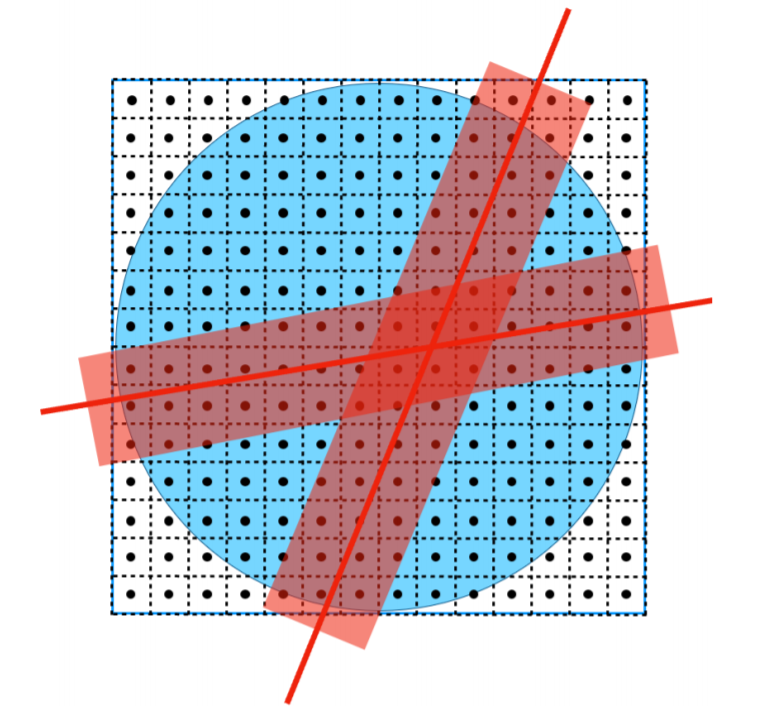
\includegraphics[width=0.5\linewidth]{4_efficiency/xyzframe_sketch.png}
    \caption{Sketch of XYZFrame method for the calculation of the SPN veto efficiency.}
    \label{fig:xyzframe_sketch}
\end{figure}

% \begin{figure}
%     \centering
%     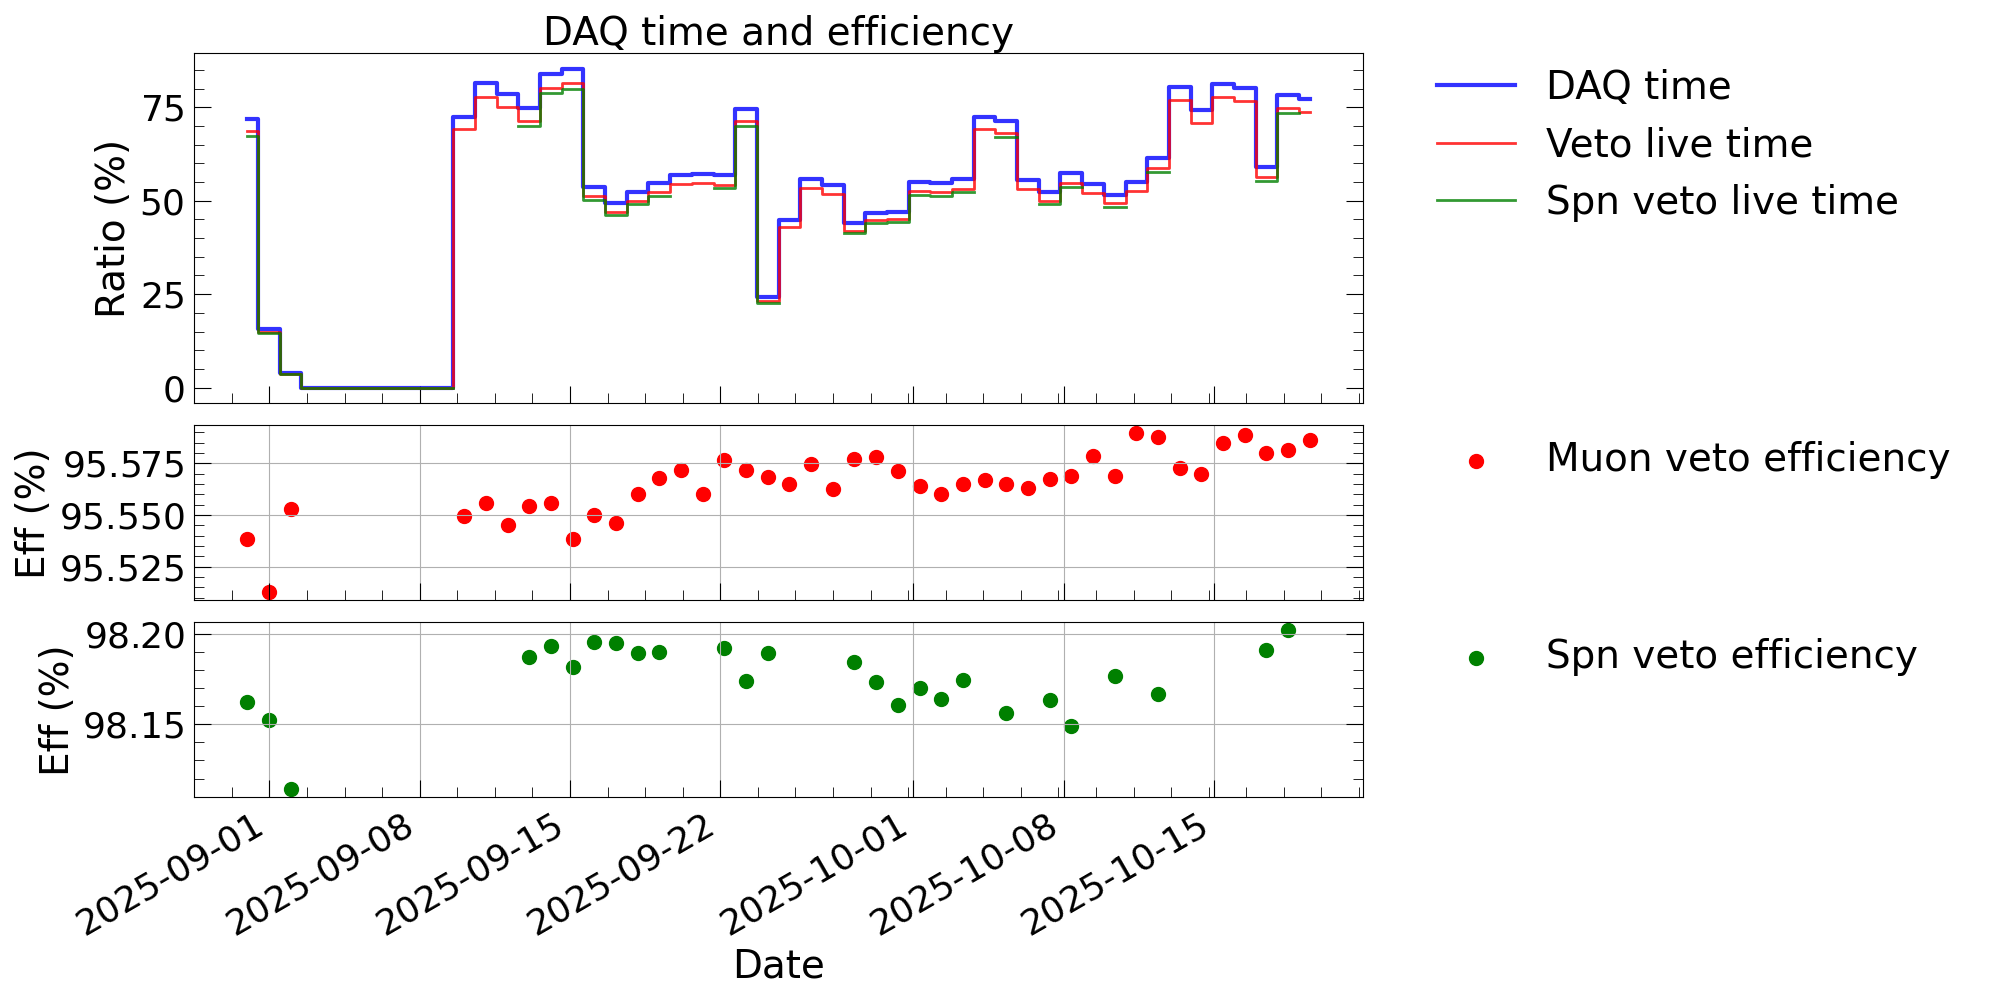
\includegraphics[width=0.95\linewidth]{4_efficiency/muon_spn_veto_eff.png}
%     \caption{Time variation of calculated muon veto and SPN veto efficiency (updating).}
%     \label{fig:muon_spn_veto_eff}
% \end{figure}


\subsubsection{Multiplicity cut}
In principle, the multiplicity cut efficiency can be calculated with the single rate analytically:
\begin{equation}
    \epsilon_{m} = e^{-(3R_{s}+3R_{c}+R_{\mu})T_{\rm corr}} \left( \int^{T_{\rm veto}}_{0} R_{\mu} e^{-R_{\mu}t_{1}} e^{-\int^{T^{\rm veto}}_{T_{\rm veto}-t_{1}} f(t_{2})dt_{2} } dt_{1} + e^{-R_{\mu}T_{\rm veto}} \right)
    \label{eq:multi_eff_cal}
\end{equation}

The efficiency also can be calculated with live time method with negligible uncertainty, as shown in Fig. \ref{fig:multi_eff_cal} [DocDB-14397].
Fig. \ref{fig:multi_eff_vs_time} shows the calculated results.

\begin{figure}
    \centering
    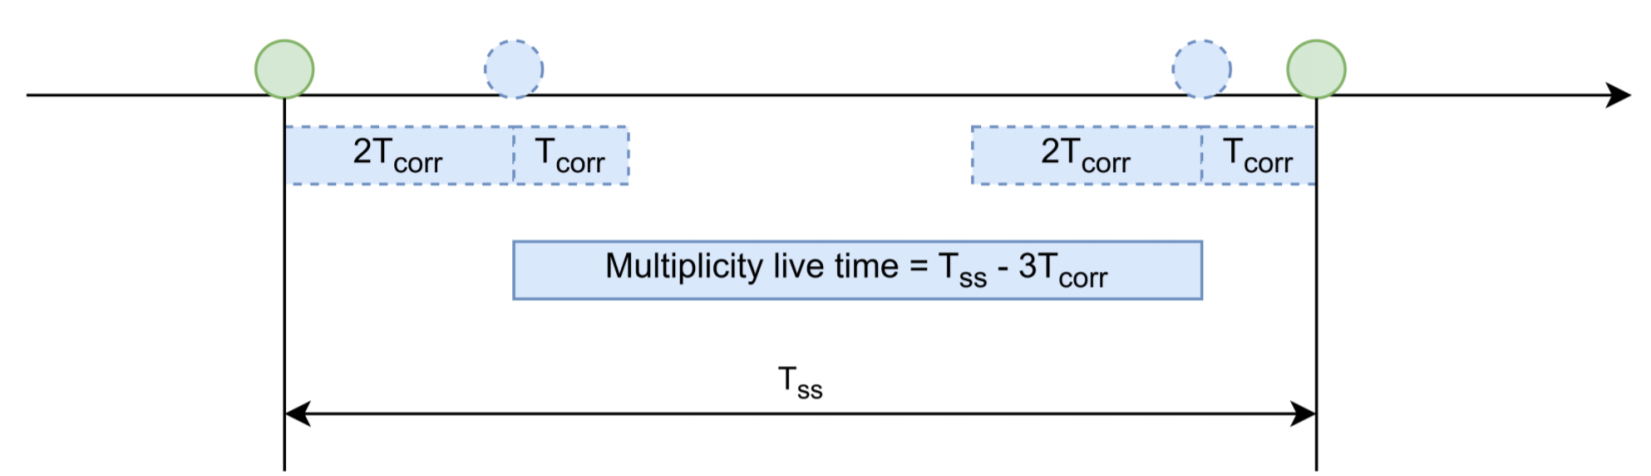
\includegraphics[width=0.95\linewidth]{4_efficiency/multi_eff_cal.png}
    \caption{Sketch for the calculation of the multiplicity cut efficiency. Green solid circles represent real events, and bule dashed circles imaginary signals.}
    \label{fig:multi_eff_cal}
\end{figure}

\begin{figure}
    \centering
    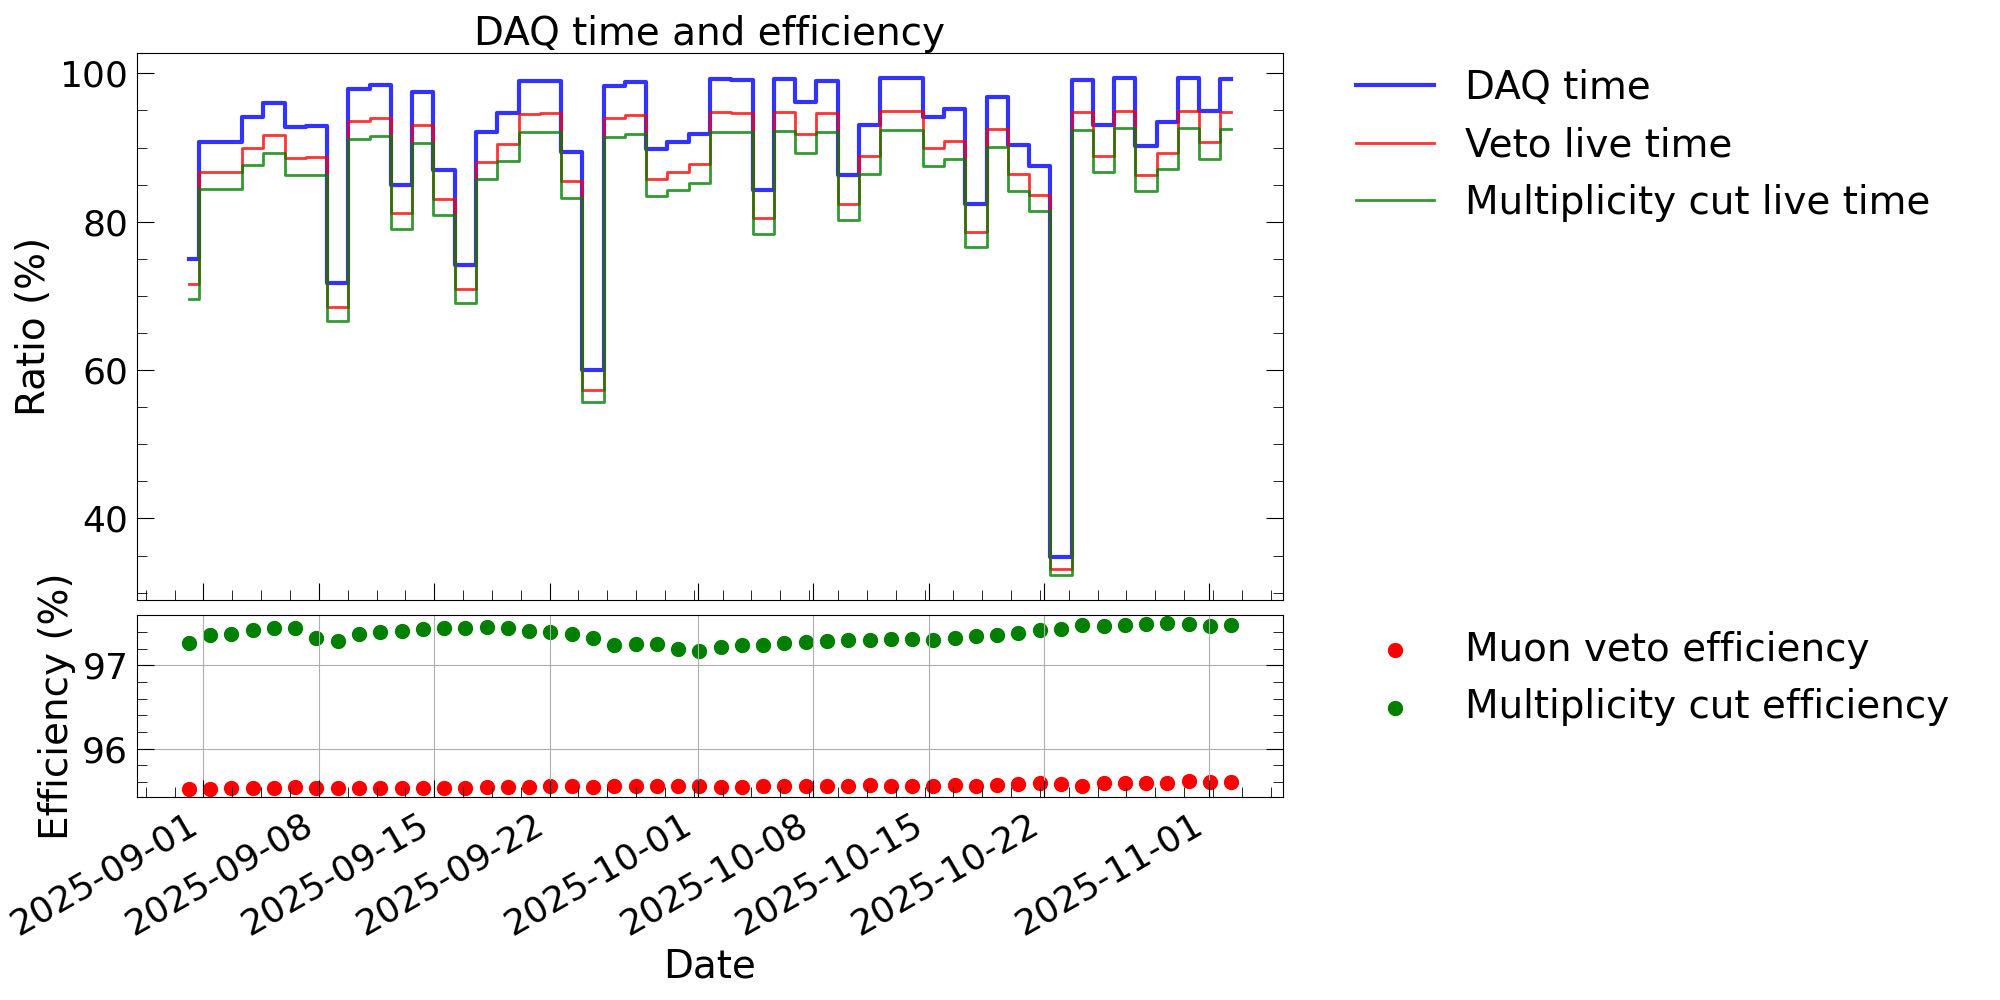
\includegraphics[width=0.95\linewidth]{4_efficiency/multi_eff_vs_time.jpg}
    \caption{Time variation of calculated multiplicity cut efficiency.}
    \label{fig:multi_eff_vs_time}
\end{figure}


\subsubsection{Prompt energy cut}
The prompt energy of IBDs is constrained within (0.7, 12) MeV. The in-efficiency mainly comes from two parts: energy leakage and energy resolution.

With the tight FV cut, the energy leakage effect is negligible, as confirmed with MC samples and shown in \ref{fig:ep_mc_all}, \ref{fig:ep_mc_169} and \ref{fig:ep_mc_165}.

\begin{figure}[h]
  \centering
  \begin{subfigure}[t]{0.32\textwidth}
    \centering
    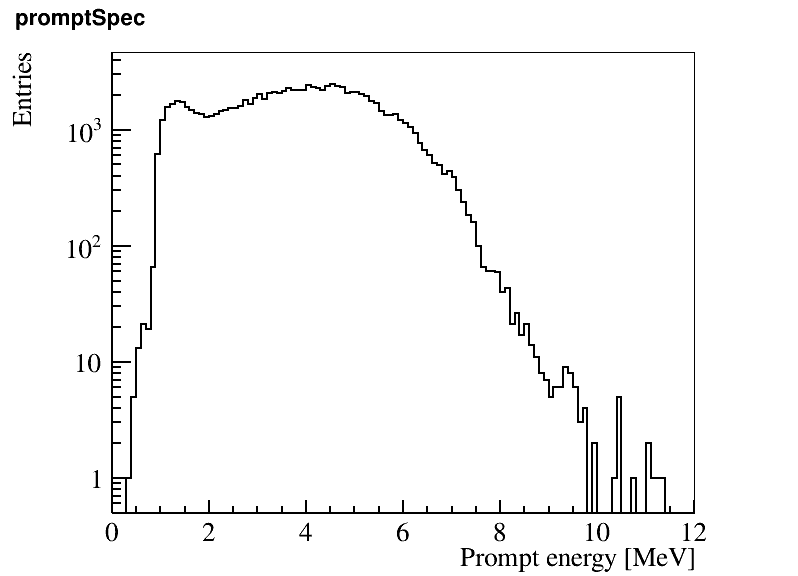
\includegraphics[width=\linewidth]{4_efficiency/promptSpec_logy_mc_ibd_all.png}
    \caption{}
    \label{fig:ep_mc_all}
  \end{subfigure}
  \hfill
  \begin{subfigure}[t]{0.32\textwidth}
    \centering
    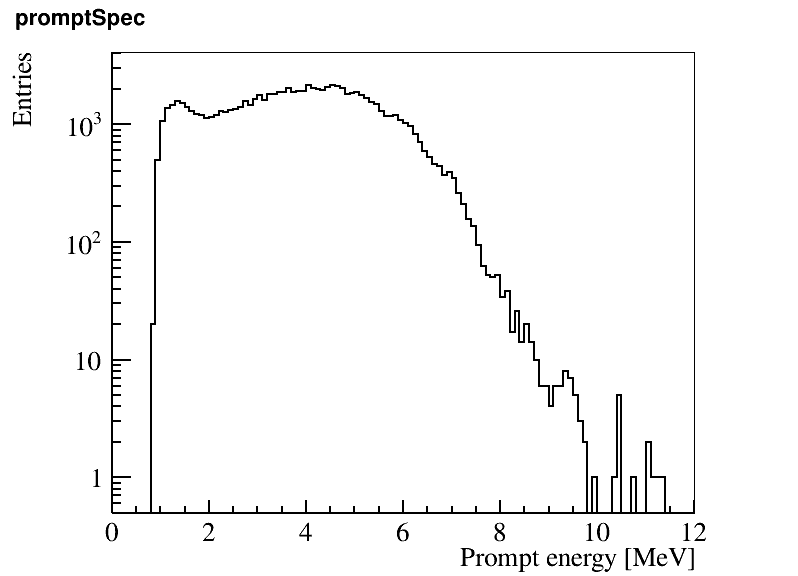
\includegraphics[width=\linewidth]{4_efficiency/promptSpec_logy_mc_ibd_169.png}
    \caption{}
    \label{fig:ep_mc_169}
  \end{subfigure}
  \hfill
  \begin{subfigure}[t]{0.32\textwidth}
    \centering
    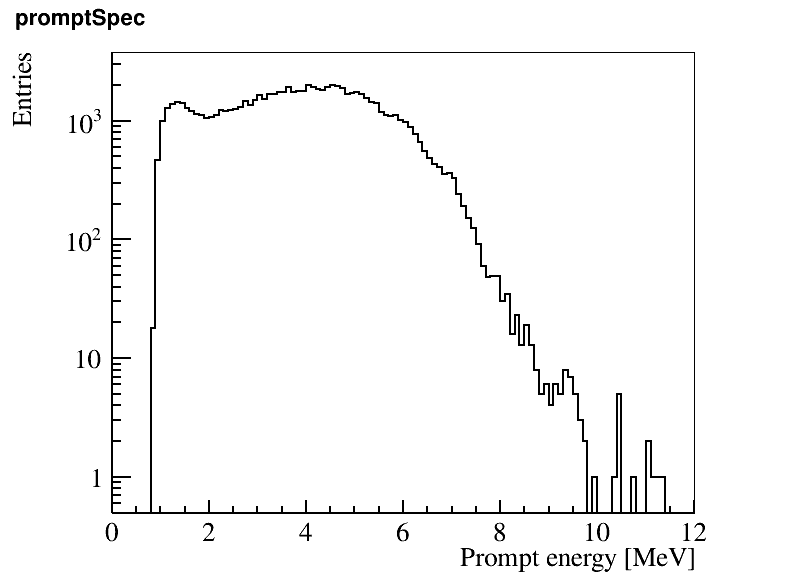
\includegraphics[width=\linewidth]{4_efficiency/promptSpec_logy_mc_ibd_165.png}
    \caption{}
    \label{fig:ep_mc_165}
  \end{subfigure}
  \caption{Prompt spectra of MC IBDs with different FV cuts: (a) no FV cut, (b) FV < 16.9 m and (c) FV < 16.5 m.}
\end{figure}

To study the in-efficiency caused by the energy resolution, we use calibration data of Ge68 source with two 0.511 MeV $\gamma$s emitted, which is corresponding to the lowest energy of IBDs without energy leakage.
As shown in the Fig. \ref{fig:Ge68_spec_x0y0z0_fit}, one single Gaussian function is used in the fitting to get the peak energy $\mu$ and resolution $\sigma$.
Then the lowest reconstructed prompt energy is estimated as $\sim$ 0.77 MeV for OEC energy and $\sim$ 0.75 MeV for OMILREC energy, which are both higher than the energy threshold of 0.7 MeV.

\begin{figure}
    \centering
    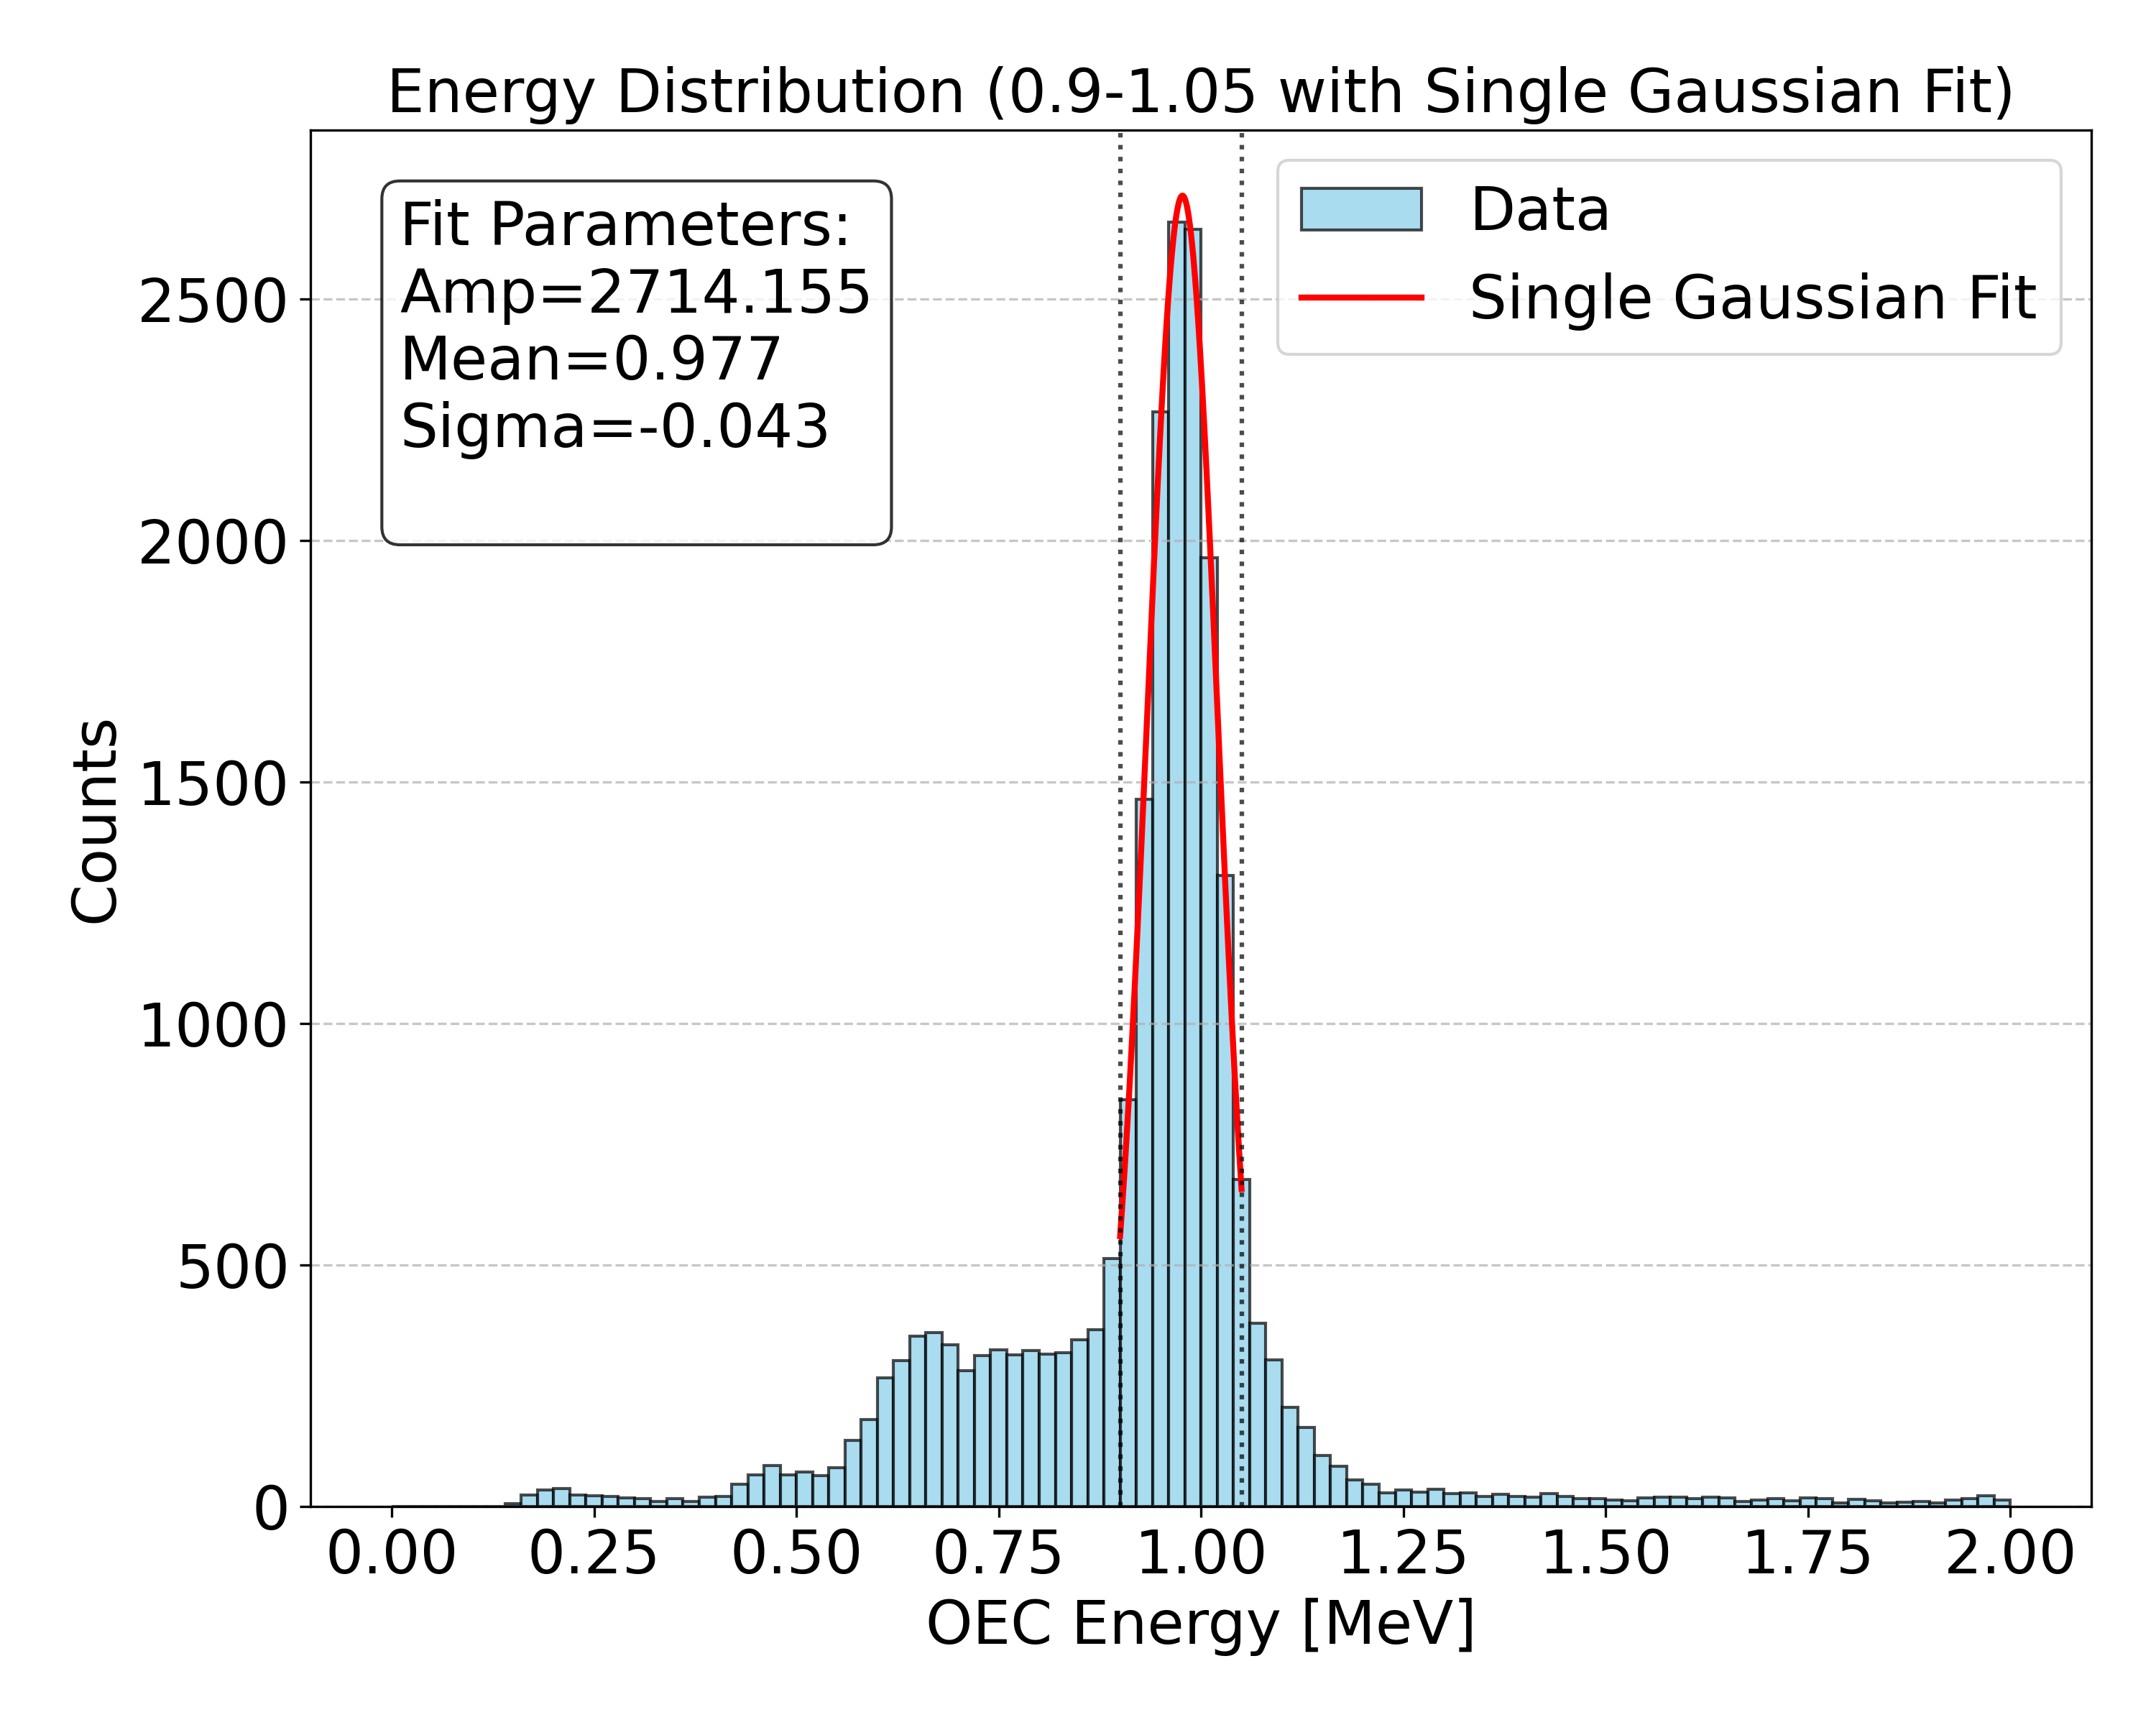
\includegraphics[width=0.5\linewidth]{4_efficiency/Ge68_spec_x0y0z0_fit.png}
    \caption{Energy spectrum of $^{68}$Ge source at CD center. The full-energy peak is fitted with single Gaussian function.}
    \label{fig:Ge68_spec_x0y0z0_fit}
\end{figure}

In summary, the in-efficiency and the corresponding uncertainty of prompt energy cut are both negligible in our selections.

\subsubsection{Delayed energy cut}
As discussed in the previous section and shown in Fig. \ref{fig:ed_mc_all}, \ref{fig:ed_mc_169} and \ref{fig:ed_mc_165}, the energy leakage effect is negligible with this tight FV cut.
Thus, we use a single Gaussian function to fit the delayed spectrum, as shown in Fig. \ref{fig:delayedSpec_ibd}.
Then the efficiency of delayed energy cut is calculated with the fitting function as 
\begin{equation}
    \epsilon_{ed} = \frac{N(2.0~{\rm MeV} < E_{d} < 2.5~{\rm MeV})}{N(\text{Without Ed cut})} = 99.99\%
    \label{eq:ed_eff}
\end{equation}

\begin{figure}[h]
  \centering
  \begin{subfigure}[t]{0.32\textwidth}
    \centering
    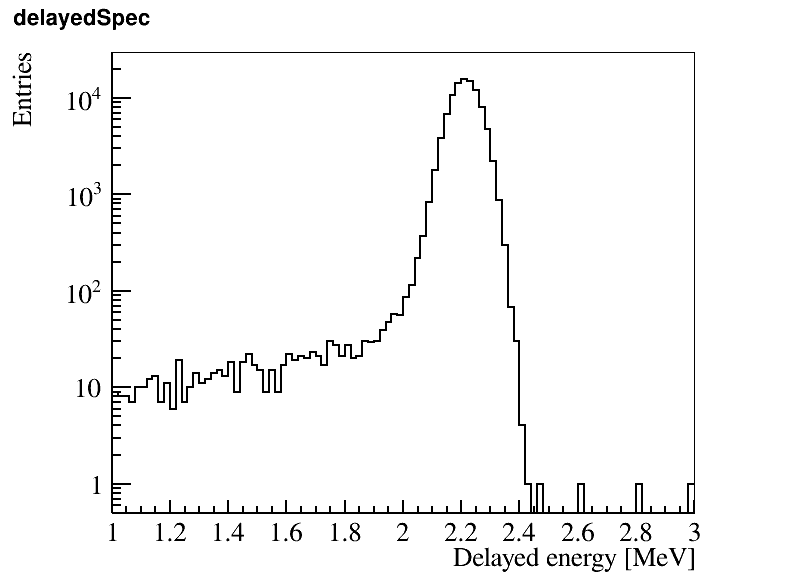
\includegraphics[width=\linewidth]{4_efficiency/delayedSpec_logy_mc_ibd_all.png}
    \caption{}
    \label{fig:ed_mc_all}
  \end{subfigure}
  \hfill
  \begin{subfigure}[t]{0.32\textwidth}
    \centering
    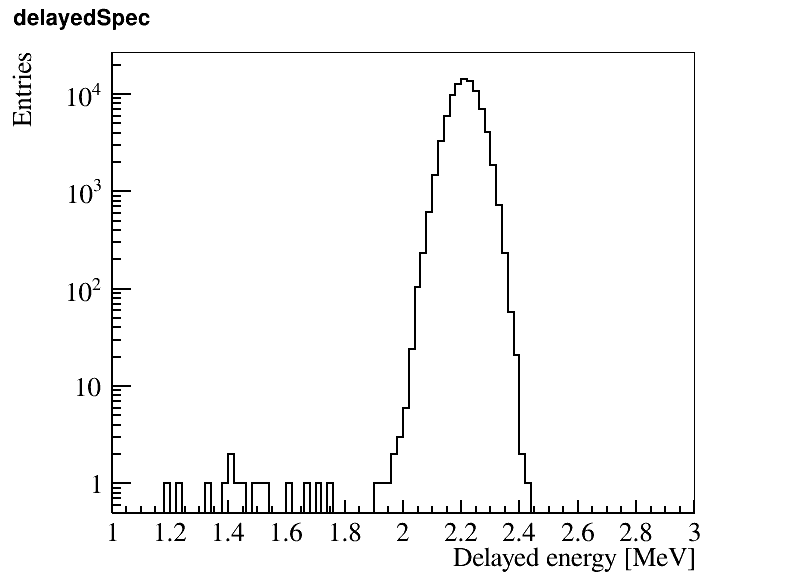
\includegraphics[width=\linewidth]{4_efficiency/delayedSpec_logy_mc_ibd_169.png}
    \caption{}
    \label{fig:ed_mc_169}
  \end{subfigure}
  \hfill
  \begin{subfigure}[t]{0.32\textwidth}
    \centering
    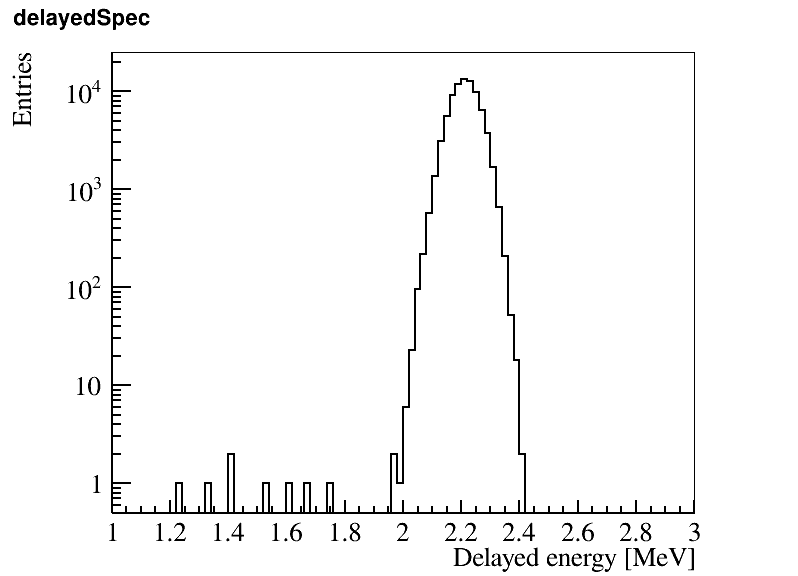
\includegraphics[width=\linewidth]{4_efficiency/delayedSpec_logy_mc_ibd_165.png}
    \caption{}
    \label{fig:ed_mc_165}
  \end{subfigure}
  \caption{Delayed spectra of MC IBDs with different FV cuts: (a) no FV cut, (b) FV < 16.9 m and (c) FV < 16.5 m. Significant energy leakage is found without any FV cut and negligible effect exists with FV < 16.9 m or FV < 16.5 m.}
\end{figure}

The analysis of the corresponding systematic uncertainty is still under way. 
It mainly comes from the fitting strategy and energy response related uncertainty which will lead to the distortion of spectrum shape.
Since the efficiency is high enough, the systematic uncertainty is set to 0.1\% directly.

\begin{figure}
    \centering
    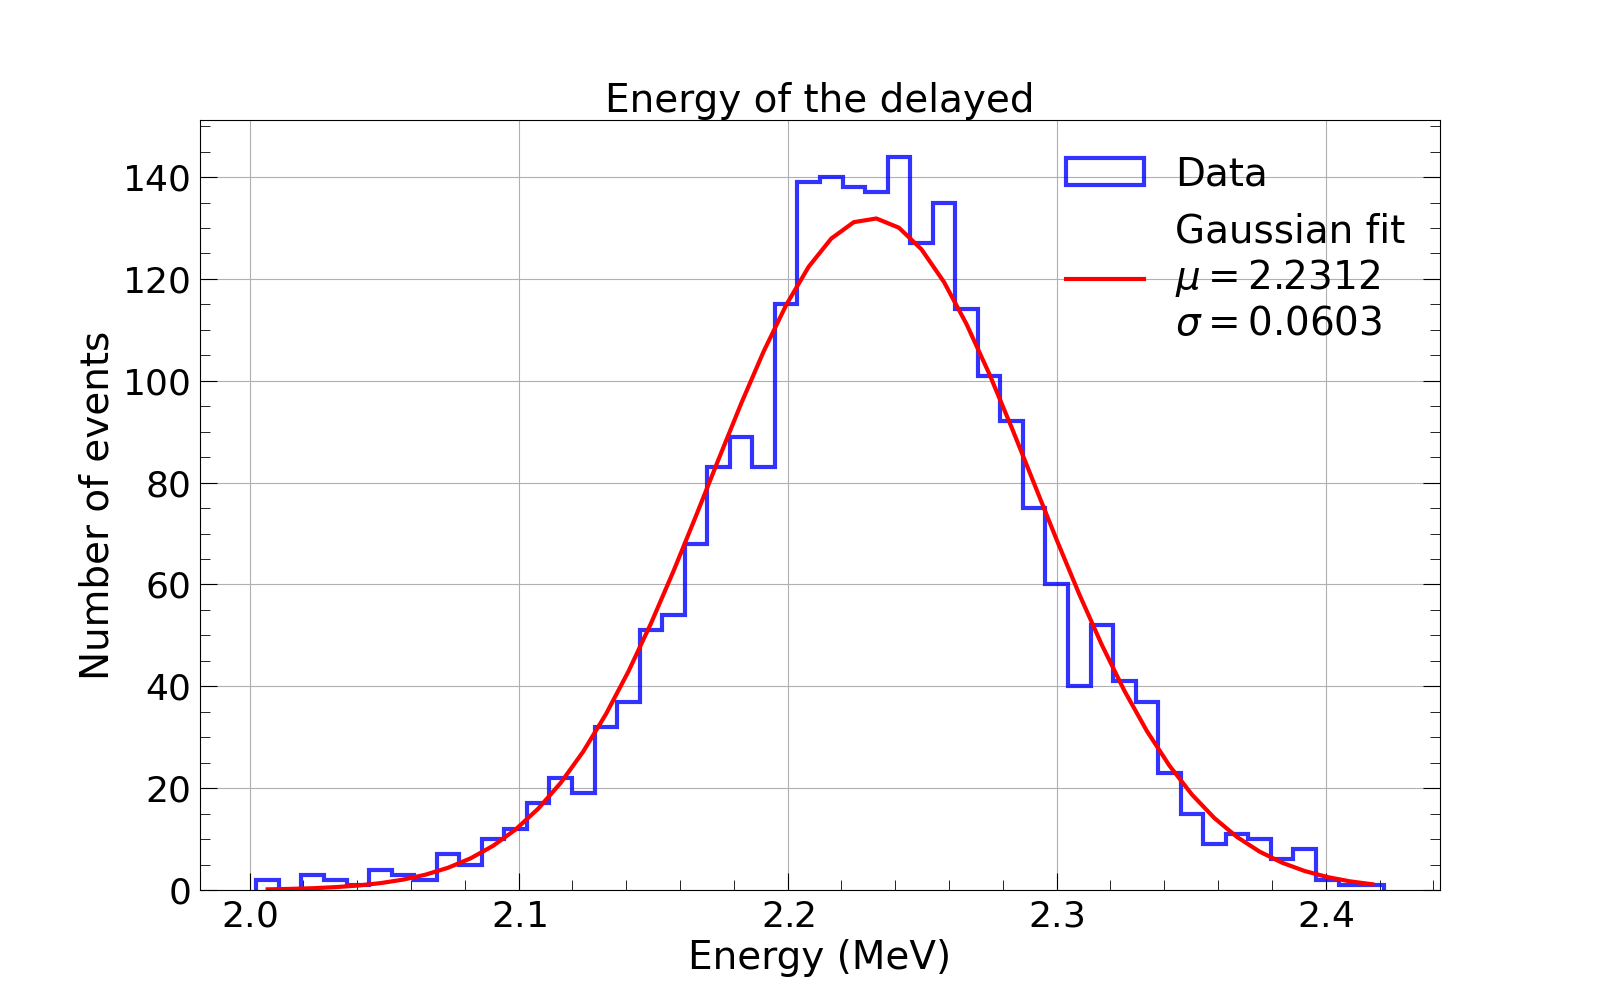
\includegraphics[width=0.5\linewidth]{2_selection/h_ibd_e_d.png}
    \caption{Delayed spectrum of IBD candidates. The data is fitted with single Gaussian function.}
    \label{fig:delayedSpec_ibd}
\end{figure}

Noting that the efficiency estimation is based on the OEC energy, the efficiency for OMILREC reconstruction will be re-calculated once enough re-production data and fine-tuning MC samples are ready.


\subsubsection{Time interval cut}
The time interval between prompt and delayed signals are composed of two parts, neutron thermalization ($\sim$ 4 $\mu$s) and neutron capture on hydrogen (nH) ($\sim$ 220 $\mu$s).
As a preliminary study, we neglect the contribution from the thermalization which is much faster compared to neutron capture and has small effect on the estimation of the efficiency.
In this case, the time constant should be identical for AmC and IBD.
By fitting the time interval distribution, the time constant $\tau$ can be obtained from these two samples, as shown in Fig. \ref{fig:dt_ibd} and Fig. \ref{fig:dt_AmC}. Then, the efficiency of dt cut can be calculated with the fitting function as
\begin{equation}
    \epsilon_{dt} = \frac{N(5~\mu s<dt<1000~\mu s)}{N(\text{Without dt cut})} = 96.80\%
    \label{eq:dt_eff}
\end{equation}

\begin{figure}[h]
  \centering
  \begin{subfigure}[t]{0.45\textwidth}
    \centering
    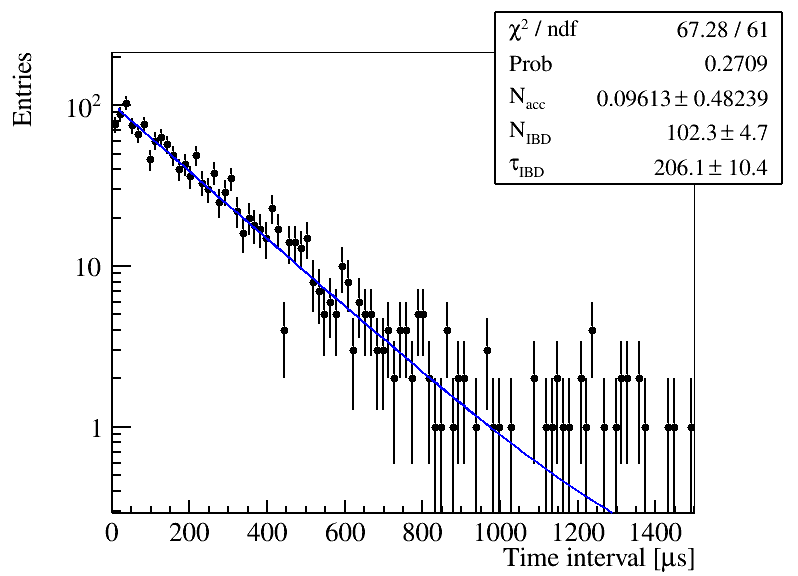
\includegraphics[width=\linewidth]{4_efficiency/dt_ibd.png}
    \caption{}
    \label{fig:dt_ibd}
  \end{subfigure}
  \hfill
  \begin{subfigure}[t]{0.45\textwidth}
    \centering
    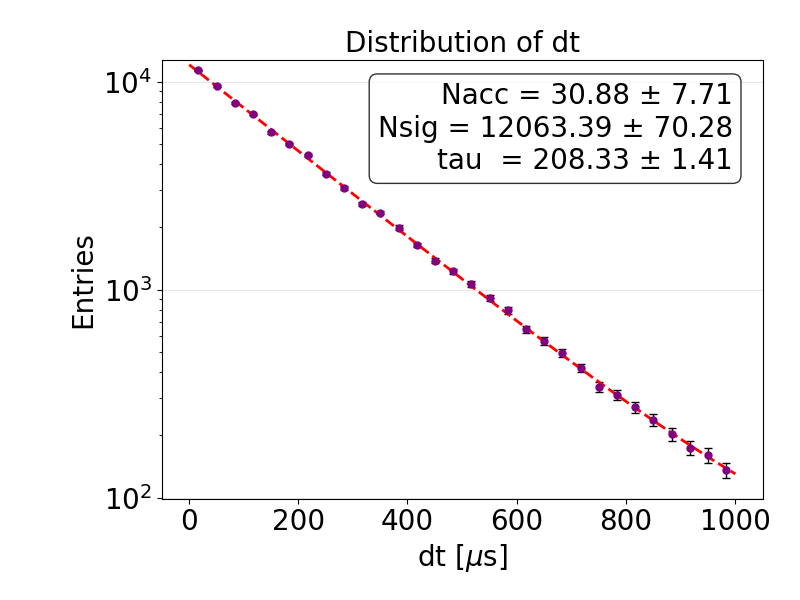
\includegraphics[width=\linewidth]{4_efficiency/dt_AmC_fit.png}
    \caption{}
    \label{fig:dt_AmC}
  \end{subfigure}
  \caption{Time interval distribution of (a) IBDs and (b) AmC correlated events. The data is fitted with an exponential decay function plus an constant.}
\end{figure}

The systematic uncertainty mainly comes from the time precision ($\sim$ 8 ns) and the fitting error of the time constant.
The time precision has negligible effect on the efficiency.
For the second factor, we compared the fitting time constant $\tau$ with AmC and IBD samples, and found the relative difference as $\sim$ 1\%. Then, it leads to the relative difference of the efficiency as $\sim$ 0.02\%, which is taken as the systematic uncertainty.


\subsubsection{Relative distance cut}
In this section, we use IBD candidate sample to estimate the efficiency of relative distance (dr) cut. 

To make an unbiased estimation, backgrounds should be removed from the sample.
After the standard IBD selection, the main backgrounds include Li9, geo-neutrinos, world reactor neutrinos, accidental background and so on. Geo-neutrinos and world reactor neutrinos have the same dr distribution as IBDs', which has not effect on the estimation.
As shown in Fig. \ref{fig:dr_ibd_li9_amc_mc}, IBD and Li9 have the same distribution of relative distance within the uncertainty. Thus, it's acceptable to reserve Li9 in the sample as well. 
However, the dr distribution of accidental background is flat, which will bias the estimation.
To remove this background, more strict selections are applied: $E_p$ > 1.5 MeV, and $dt$ < 600 $\mu$s.
For comparison, distributions of MC IBD [DocDB-13483] and AmC are shown in Fig. \ref{fig:dr_ibd_li9_amc_mc} as well. 

\begin{figure}
    \centering
    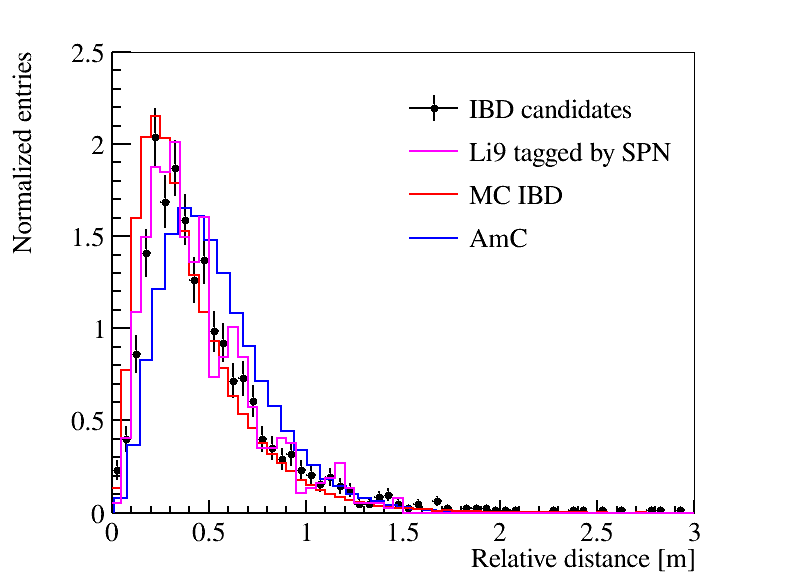
\includegraphics[width=0.5\linewidth]{4_efficiency/dr_ibd_li9_amc_mc.png}
    \caption{Relative distance distribution of IBD candidates with strict selections (black points), Li9 tagged by SPN (magenta line), MC IBDs (red line) and AmC correlated events (blue line).}
    \label{fig:dr_ibd_li9_amc_mc}
\end{figure}

With the above sample, the efficiency could be estimated as
\begin{equation}
    \epsilon_{dr} = \frac{N(dr<1.5~{\rm m})}{N(dr<3~{\rm m})} = 98.28\%
    \label{eq:dr_eff}
\end{equation}
According to MC studies, all IBDs have the relative distance dr < 3 m. Meanwhile, larger upper limit of the denominator in Eq. \ref{eq:dr_eff} will include more backgrounds and then leads to biased results.

The systematic uncertainty is estimated as the relative difference between IBD candidate and MC samples, which leads to 0.1\% uncertainty.


\subsubsection{Hydrogen-carbon capture ratio}
Inside LS region, IBD neutrons will be captured by hydrogens (nH) or carbons (nC), while in this technote only nH events are used.
To figure out the hydrogen-carbon capture ratio $\epsilon_{\text{nHCap}}$, we select AmC events with larger delayed energy region extending to 6 MeV, as shown in Fig. \ref{fig:full_delayed_spec_AmC}.
Then the ratio is estimated as
\begin{equation}
    \epsilon_{\text{nHCap}} = \frac{N(E_d<\text{3 MeV})}{N_{\text{total}}} = 99.32\% \pm 0.19\% (\text{stat.})
    \label{eq:nH_cap_ratio}
\end{equation}
The effect on the oscillation fitting results from the capture ratio is negligible (see in the section for the oscillation analysis), so it's neglected in the first physics paper.

\begin{figure}
    \centering
    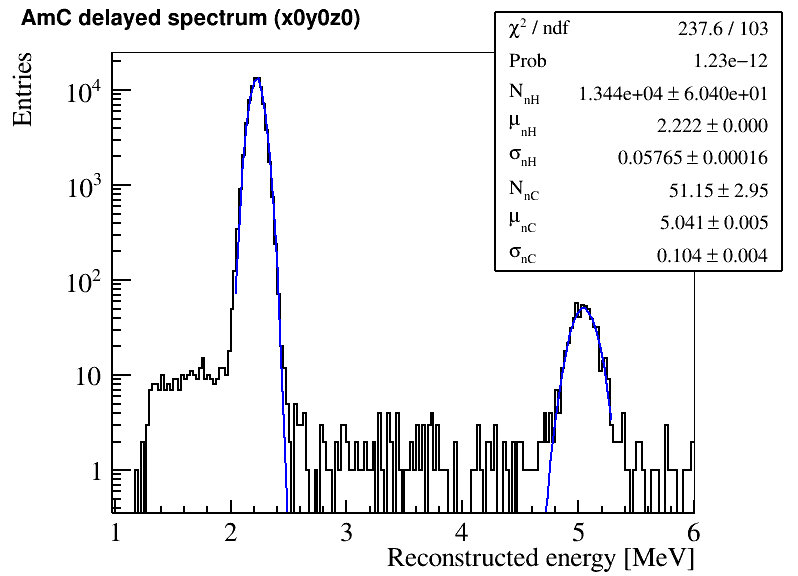
\includegraphics[width=0.5\linewidth]{4_efficiency/full_delayed_spec_AmC.png}
    \caption{Full delayed spectrum of AmC source.}
    \label{fig:full_delayed_spec_AmC}
\end{figure}


\subsubsection{Spill-in and spill-out effects}
If IBD reaction happen outside LS but near the edge of internal surface of acrylic vessel, the $\gamma$s from this electron-positron annihilation and the corresponding neutron may enter the LS region and contribute to the signal samples. However, since we only treat LS as the target volume, this contribution is not included in the prediction and should be considered separately. In this note, we call it spill-in effect.

Generally, IBD positron will deposite energy locally with only few millimeters displacement, while the $\gamma$s from this electron-positron annihilation will travel a few tens of cm. Besides, IBD neutrons take a few cm to be thermalized and the 2.2 MeV $\gamma$ from neutron capture travels a few tens of cm. Fortunately, since the edge of FV is far away from the internal surface of acrylic vessel ($\sim$ 1.2 m), these events can't reach the FV.
In short, spill-in effect is negligible, thanks to the tight FV cut.

For spill-out effect, $\gamma$s from the electron-positron annihilation and neutron go outside LS region. This effect has been included in the energy leakage effect.

These effects will be re-evaluated once the fine-tuning MC samples is ready.


\subsubsection{Summary}
Detector related systematic uncertainties for neutrino flux are summarized in \ref{tab:DetErr}.

\begin{table}[!htbp]
    \caption{Summary of detector related systematic uncertainties for neutrino flux in JUNO only analysis.}
    \label{tab:DetErr}
    \centering
    \footnotesize% fontsize
    \setlength{\tabcolsep}{4pt}% column separation
    \renewcommand{\arraystretch}{1.2}%row space 
    \begin{tabular}{lcc}
        \hline
         & Efficiency & Relative uncertainty \\ 
        \hline
        Proton number & - & 1\% \\
        Flasher cut & > 99.9\% & Negligible \\
        FV cut & 80.57\% & 1.6\% \\ 
        Prompt energy cut & 100\% & Negligible \\
        Delayed energy cut & 99.99\% & 0.1\% \\
        CD and WP muon veto & 95.55\% & Negligible \\
        Multiplicity cut & 97.36\% & Negligible \\
        Spallation neutron veto & 98.00\% & Negligible \\
        Coincidence time cut  & 96.80\% & 0.02\% \\
        Relative distance cut & 98.28\% & 0.10\% \\
        nH-nC ratio (neglect in first physics paper) & 99.32\% & 0.19\% \\
        \hline
        Total & 69.88\% & 1.89\% \\
        \hline
    \end{tabular}
\end{table}



\subsection{Energy response}

As shown in Fig.~\ref{fig:Energy_response_process}, the energy response of LS exhibits a non-linear dependence on the deposited energies of charged particles, primarily owing to ionization quenching and Cherenkov radiation effects. Additional non-linearity may arise during the PMT charge reconstruction process. Generally, dispersion and fluctuations occur in each stage of the energy response and detection process, collectively contributing to the overall energy resolution.

\begin{figure}[h]
    \centering
    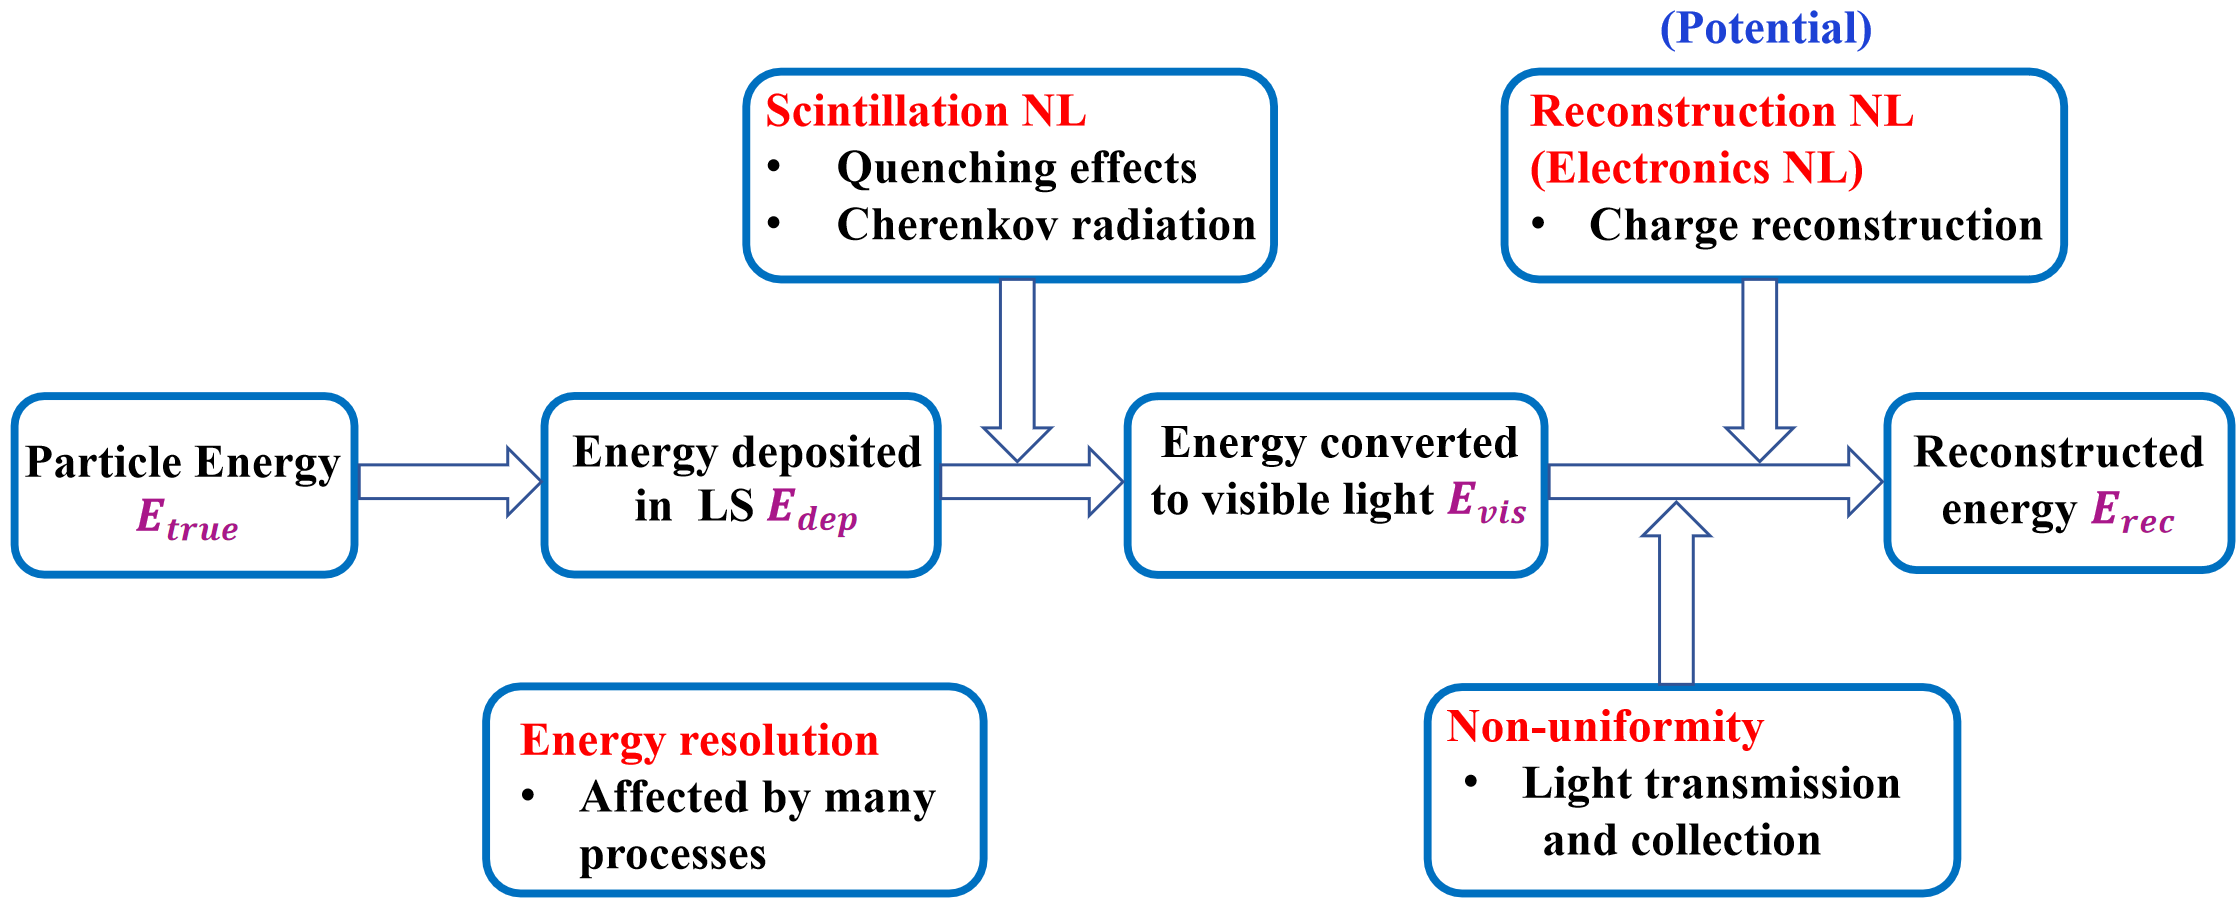
\includegraphics[width=0.9\linewidth]{4_efficiency/EnergyResponseProcess.png}
    \caption{The process of energy response.}
    \label{fig:Energy_response_process}
\end{figure}

\subsubsection{Calibration Source Selection}
\label{subsec:calibration_sources}

Table~\ref{tab:calibration_sources} summarizes the calibration sources utilized in the JUNO experiment for characterizing the energy response. These sources provide mono-energetic $\gamma$-rays and other characteristic signals across a wide energy range. The calibration strategy differs based on the source characteristics:
\begin{itemize}
    \item For \textbf{single-like events} (e.g., $\gamma$ sources like $^{137}\mathrm{Cs}$, $^{54}\mathrm{Mn}$), the event selection relies on the dynamic Fiducial Volume (FV) method described in Section~\ref{subsec:fv_selection}. Both the vertex reconstruction and energy estimation for these selections are based on the \textbf{P25C dataset}.
    \item For the AmC source, which requires identifying correlated prompt and delayed signals, an additional time coincidence selection is applied after the dynamic FV cuts to significantly reduce accidental backgrounds.
\end{itemize}

\begin{table}[h!]
\centering
\caption{Calibration sources used for energy response analysis in JUNO.}
\label{tab:calibration_sources}
\begin{tabular}{ccl}
\toprule
\textbf{Sources/Processes} & \textbf{Type} & \textbf{Radiation (MeV)} \\
\midrule
$^{137}\mathrm{Cs}$ & $\gamma$ & 0.662 \\
$^{54}\mathrm{Mn}$ & $\gamma$ & 0.835 \\
$^{60}\mathrm{Co}$ & $\gamma$ & 1.173 + 1.333 \\
$^{40}\mathrm{K}$ & $\gamma$ & 1.461 \\
$^{68}\mathrm{Ge}$ & $e^{+}$ & Annihilation 0.511 + 0.511 \\
$^{241}\mathrm{Am}$-$^{13}\mathrm{C}$ & $n, \gamma$ & $n + 6.13$ ($^{16}\mathrm{O}^{*}$) \\
$(n,\gamma)\mathrm{H}$ & $\gamma$ & 2.223 \\
$(n,\gamma)^{12}\mathrm{C}$ & $\gamma$ & 4.94 (68\%) or 3.68 + 1.26 (32\%) \\
\bottomrule
\end{tabular}
\end{table}

\paragraph{Dynamic Fiducial Volume Selection}
\label{subsec:fv_selection}

A data-driven approach is employed to define a run-dependent and source-position-dependent Fiducial Volume (FV) for each calibration run. This dynamic FV selection optimizes the signal-to-background ratio (S/B) by comparing the event distributions in both energy and spatial domains between the calibration data and a dedicated background run. A fundamental pre-selection requires all candidate events to pass a 5 ms muon veto to suppress backgrounds induced by cosmic-ray muons.

The dynamic FV selection algorithm proceeds sequentially through three dimensions:

\begin{enumerate}
    \item \textbf{Energy Region Selection:} The reconstructed energy spectrum ($E_{\mathrm{rec}}$) of the calibration run is compared with the background spectrum from one physic run. The relative difference, defined as $R_{\mathrm{diff}} = 100\% \times (N_{\mathrm{run}} - N_{\mathrm{bkg}})/N_{\mathrm{bkg}}$, is computed across energy bins. A threshold is set at the median of all $R_{\mathrm{diff}}$ bins, and a scanning algorithm identifies the contiguous energy region where $R_{\mathrm{diff}}$ consistently exceeds this threshold. This defines the optimal energy window for spatial selection in the following, typically centered around the expected $\gamma$-ray peak.
    \item \textbf{Radial ($\rho = \sqrt{x^2 + y^2}$) Constraint:} Using events within the selected energy range, the same $R_{\mathrm{diff}}$ method is applied to the radial distribution. The algorithm scans outward from $\rho = 0$ to find the radius $\rho_{\mathrm{max}}$ where $R_{\mathrm{diff}}$ drops below its mean value. This $\rho_{\mathrm{max}}$ defines the maximum radial extent of the FV for that run.
    \item \textbf{Longitudinal ($Z$) Constraint:} Events satisfying the previous energy and radial cuts are used to analyze the distribution of the reconstructed $Z$ coordinate relative to the expected source position $Z_{\mu}$. The $R_{\mathrm{diff}}$ thresholding yields $Z_{\mathrm{max}}$, the maximum allowed absolute deviation $|Z - Z_{\mu}|$ along the longitudinal axis.
\end{enumerate}

\begin{figure}[h!]
    \centering
    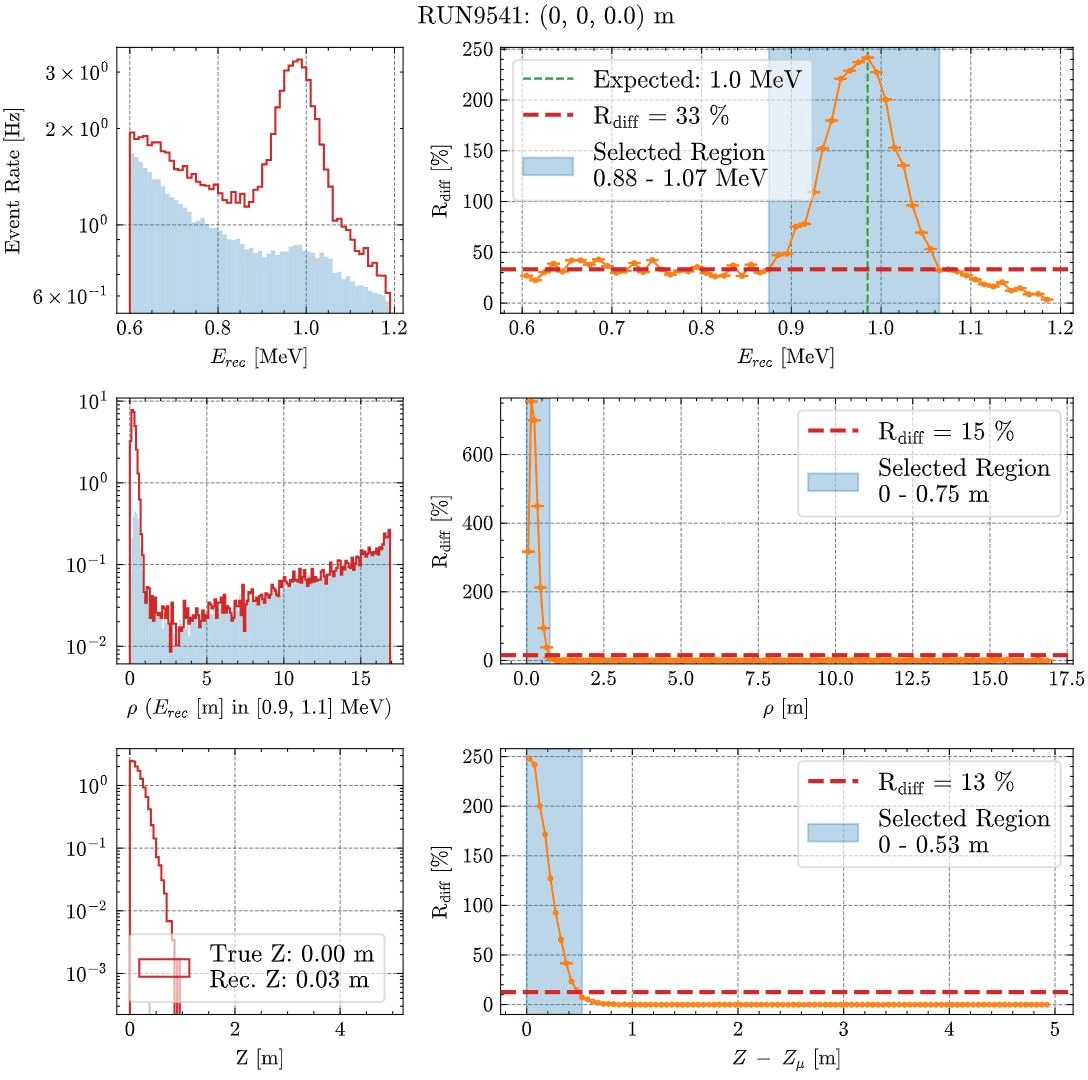
\includegraphics[width=0.8\textwidth]{4_efficiency/Ge68_FV_selection.png}
    \caption{Example of the dynamic Fiducial Volume selection for a central $^{68}$Ge run (RUN9541). \textbf{(Top)}: Energy spectra of the calibration run (red) and background (blue). \textbf{(Bottom)}: Relative difference $R_{\mathrm{diff}}$ with the selected energy region highlighted. The median $R_{\mathrm{diff}}$ threshold is shown as a red dashed line.}
    \label{fig:energy_selection}
\end{figure}

The final FV is defined by an elliptical cut based on the determined $\rho_{\mathrm{max}}$ and $Z_{\mathrm{max}}$. An event passes the FV cut if it satisfies the following condition:
$$
\sqrt{ \left(\frac{\rho}{\rho_{\mathrm{max}}}\right)^2 + \left(\frac{Z - Z_{\mu}}{Z_{\mathrm{max}}}\right)^2 } \leq 1
$$
where $\rho$ is the radial coordinate of the event and $Z$ is its longitudinal coordinate. The entire process is illustrated for a central $^{68}$Ge run in Fig.~\ref{fig:energy_selection}.

\paragraph{Correlation Selection for AmC Source}
\label{subsec:amc_selection}

Among all calibration sources, only the $^{241}\mathrm{Am}$-C (AmC) neutron source necessitates additional time correlation selection to identify the characteristic signature of neutron capture: a prompt signal from neutron reecoil or excitation, followed by a delayed $\gamma$-ray emission of neutron capture. The selection criteria are summarized in Table~\ref{tab:amc_cuts}. This method is applied after the dynamic FV selection described in Section~\ref{subsec:fv_selection} to further suppress accidental coincidences.

\begin{table}[h!]
\centering
\caption{Time correlation selection criteria for the AmC neutron source.}
\label{tab:amc_cuts}
\begin{tabular}{lll}
\toprule
\textbf{Parameter} & \textbf{Value} & \textbf{Description} \\
\midrule
$\Delta t_{\mathrm{max}}$ & 1 ms & Maximum time difference between prompt and delayed signals \\
$\mu$ veto & 5 ms & Muon veto window applied to all events \\
$E_{\mathrm{prompt}}$ & 0.3--12 MeV & Energy range for the prompt signal \\
$E_{\mathrm{delayed}}$ & 1.4--12 MeV & Energy range for the delayed signal \\
$d_{\mathrm{max}}$ & 5 m & Maximum spatial separation between prompt and delayed vertices \\
\bottomrule
\end{tabular}
\end{table}

The selection algorithm involves the following steps:

\begin{enumerate}
    \item \textbf{Initial Selection:} Events passing the dynamic FV cuts and within a broad energy range of $0.3 < E_{\mathrm{rec}} < 14$ MeV are selected as candidates.
    \item \textbf{Pair Finding:} All pairs of events within the same run occurring within a time window of $\Delta t < 1$ ms are identified. To minimize combinatorial background, only pairs consisting of exactly two events (one candidate prompt, one candidate delayed) are retained.
    \item \textbf{Energy and Distance Cuts:} Each pair must satisfy the energy conditions listed in Table~\ref{tab:amc_cuts} and have a spatial separation $d < 5$ m, ensuring the signals are spatially correlated.
\end{enumerate}

The time difference ($\Delta t$) distribution of the selected candidate pairs is then analyzed. It is fitted with a function of the form $f(\Delta t) = A e^{-\Delta t/\tau} + c$, where the decay constant $\tau$ corresponds to the neutron capture time. The fitted value of $\tau \approx 209$ $\mu$s is consistent with expectations for neutron thermalization and capture in the liquid scintillator, validating the selection efficiency. The results of this procedure, including the $\Delta t$ distribution fit and the correlation between prompt and delayed event energies, are shown in Fig.~\ref{fig:amc_selection}. After applying all selection criteria, the AmC event rate is approximately 70 Hz.

\begin{figure}[h!]
    \centering
    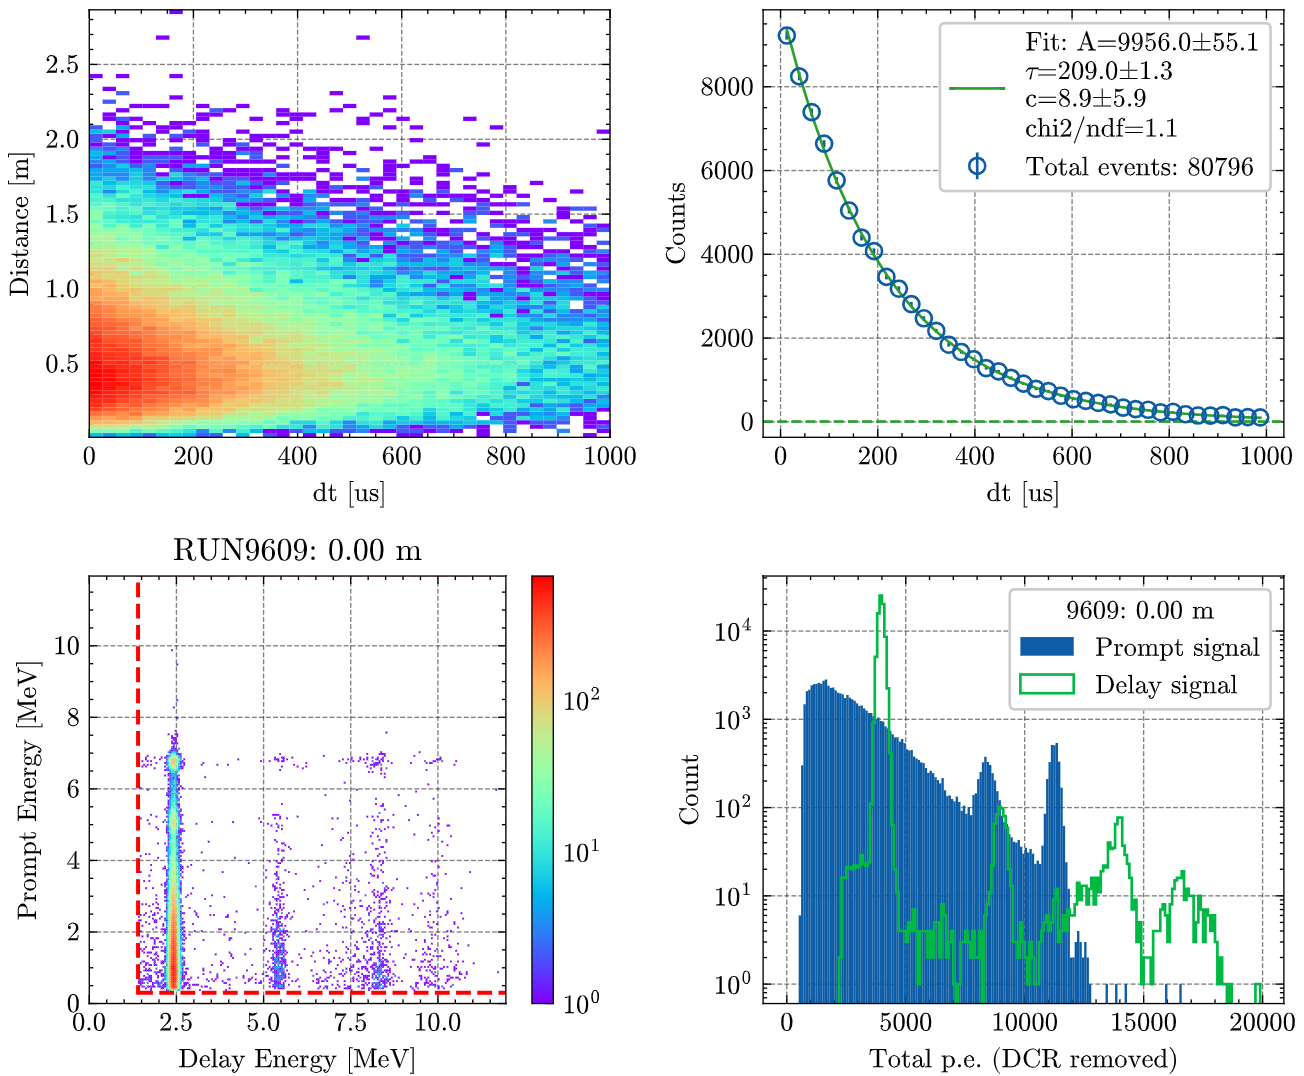
\includegraphics[width=0.9\textwidth]{4_efficiency/AmC_events.png}
    \caption{
        Comprehensive results of the time correlation selection for the AmC neutron source.
        \textbf{Top left}: The two-dimensional distribution of the time difference ($\Delta t$) versus spatial separation between candidate prompt and delayed events. The concentration of events at small $\Delta t$ and small distances is the characteristic signature of neutron capture.
        \textbf{Top right}: The projected $\Delta t$ distribution fitted with an exponential decay function plus a constant background. The extracted neutron capture time constant is approximately 200 $\mu$s, which is consistent with expectations for the liquid scintillator medium.
        \textbf{Bottom left}: The energy correlation plot between the prompt and delayed signals, revealing distinct clusters associated with different neutron interaction processes.
        \textbf{Bottom right}: The total PE energy spectra of the prompt (blue) and delayed (green) signals.
    }
    \label{fig:amc_selection}
\end{figure}

These clean samples provide crucial calibration points at several distinct energies and the energy spectrum is shown in (Fig.~\ref{fig:energy_spectrum}), which are essential for determining the energy scale and characterizing the non-linearity across the entire JUNO detector volume.
\begin{figure}[h!]
    \centering
    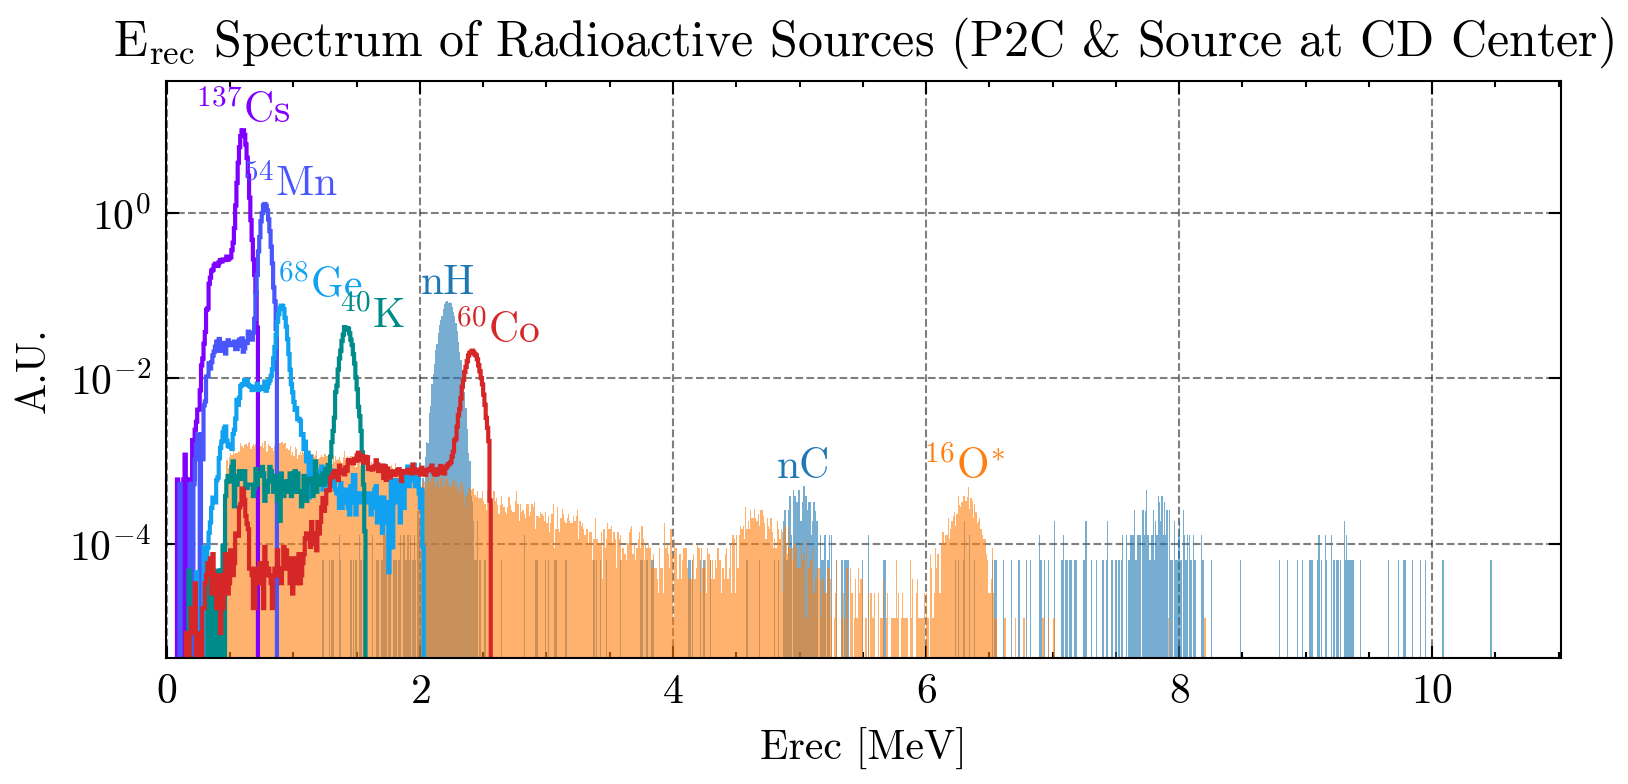
\includegraphics[width=0.9\textwidth]{4_efficiency/Energy_spectrum.png}
    \caption{The energy spectrum from various calibration sources after corresponding event selections}
    \label{fig:energy_spectrum}
\end{figure}

\subsubsection{Spallation Neutron Selection}
\label{subsec:spn_selec}

Spallation neutrons (SPN) are neutrons produced by hadronic showers induced by cosmic-ray muons as they traverse the detector.
%
These neutrons are characterized by the emission of a 2.223~MeV $\gamma$ ray when they are captured by hydrogen after thermalization, typically occurring on a timescale of several hundred microseconds following a CDmuon event.
%
Consequently, a clean sample of SPN can serve as a valuable monitor of temporal variations in the detector energy scale and can be used to estimate the energy scale uncertainty.
%
Furthermore, SPN provide an independent cross-check of the fiducial volume cut efficiency used in physics event selections such as IBD, and allow studies of energy non-linearity as a function of the event position within the detector.

To obtain a clean SPN enriched sample, we designed the selection criteria as 
follows (Fig.~\ref{fig:spn_selec}):

\begin{itemize}
    \item \textbf{Data set}: 
    /eos/juno/juno-reprod/ReProd25C/global\_trigger

    \item \textbf{Parent CDmuon}: OEC energy larger than 200~MeV;
    at least one water-pool muon within $(-2,\,2)\,\mu\text{s}$ of the parent CDmuon;
    no events with energy larger than $20$~MeV within $(-10,\,5)$~ms of the parent CDmuon.

    \item \textbf{In-window (SPN candidate)}: time interval to the parent CDmuon within $(100,\,2000)\,\mu\text{s}$;
    fiducial volume cut $R < 16.5$~m and $\lvert Z \rvert < 15.5$~m;
    afterpulse- and flasher-tag algorithms are applied to remove non-physical events.
    
    \item \textbf{Off-window (accidental background)}: the interval $(-2000,\,-5)\,\mu\text{s}$ before the parent CDmuon, used to characterize the accidental background in the in-window.
\end{itemize}

\begin{figure}[h!]
    \centering
    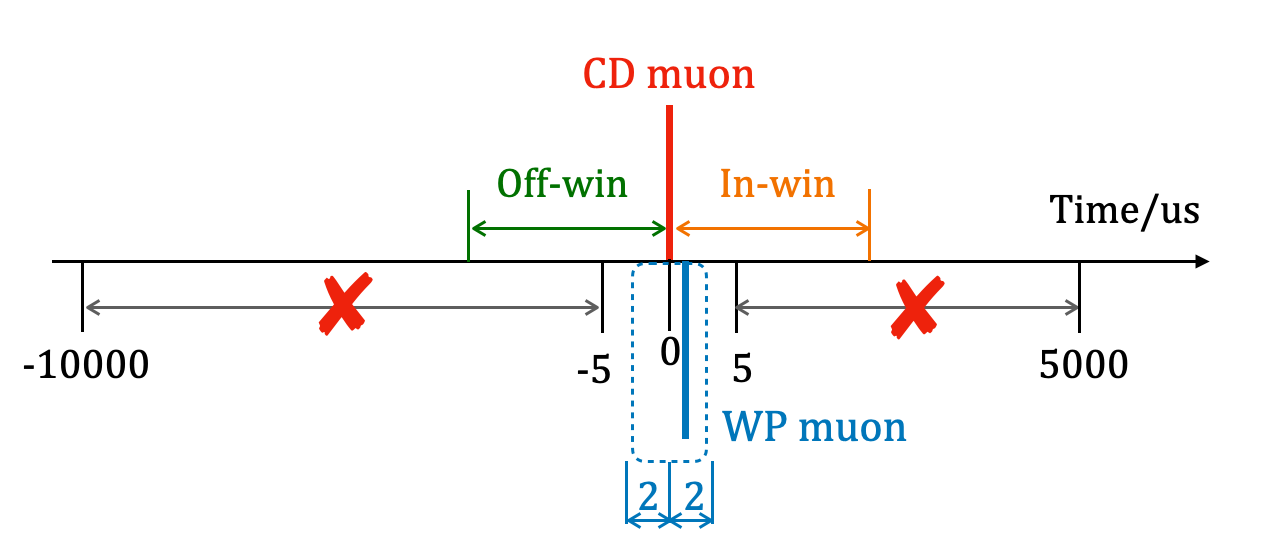
\includegraphics[width=0.9\textwidth]{4_efficiency/SPN_selection.png}
    \caption{Schematic illustration of the selection criteria for cosmogenic spallation neutron candidates.}
    \label{fig:spn_selec}
\end{figure}

In the energy spectrum and time distribution of the selected SPN enriched sample, the contributions from afterpulses and accidental backgrounds are modelled with polynomial and constant functions, respectively, while the SPN is described by a Gaussian distribution in energy and an exponential distribution in the time difference to the parent CDmuon.
%
The fit results are presented in Fig.~\ref{fig:spnFit}, yielding a reconstructed energy peak at 2.26~MeV and a characteristic time constant of 220~$\mu$s for the spallation neutrons captured by hydrogen.
%
Furthermore, by dividing the SPN enriched sample according to data-taking periods and detector spatial regions and performing the fits separately, the SPN sample provides a monitoring of the temporal variation of the detector energy scale (Fig.~\ref{fig:energy_correction_timeline}) as well as its dependence on the event position within the detector (Fig.~\ref{fig:energy_bias_uncertainty}).

\begin{figure}[h]
    \centering
    \begin{subfigure}[t]{0.45\textwidth}
        \centering
        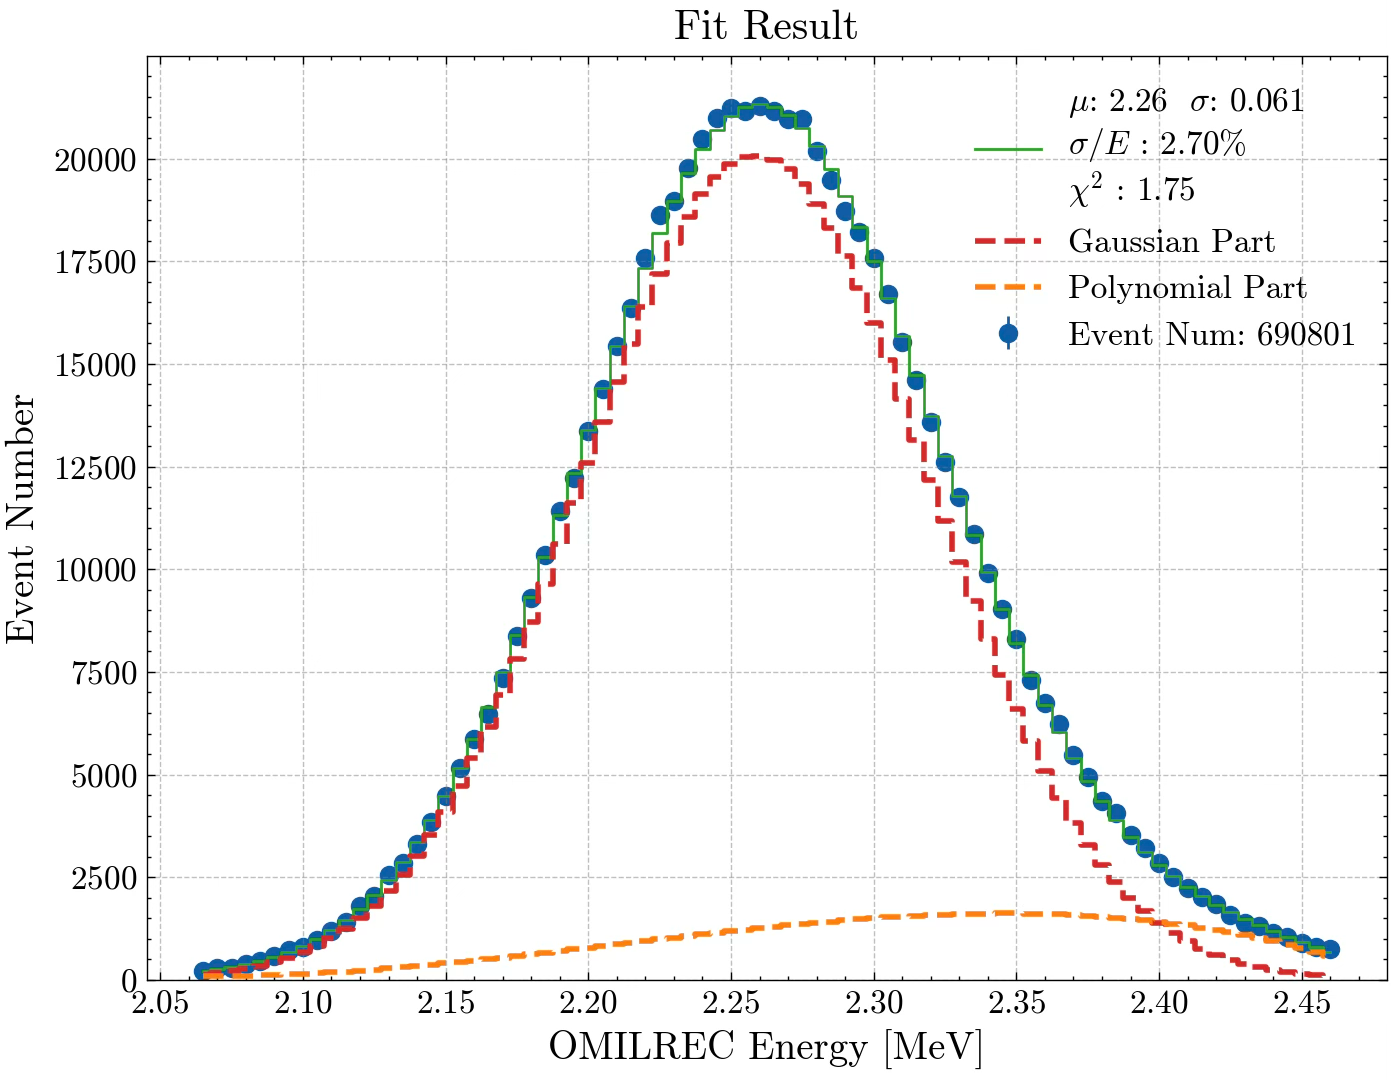
\includegraphics[width=\linewidth]{4_efficiency/SPN_energyFit.png}
        \caption{}
    \label{fig:spnEnergyFit}
    \end{subfigure}
    \hfill
    \begin{subfigure}[t]{0.45\textwidth}
        \centering
        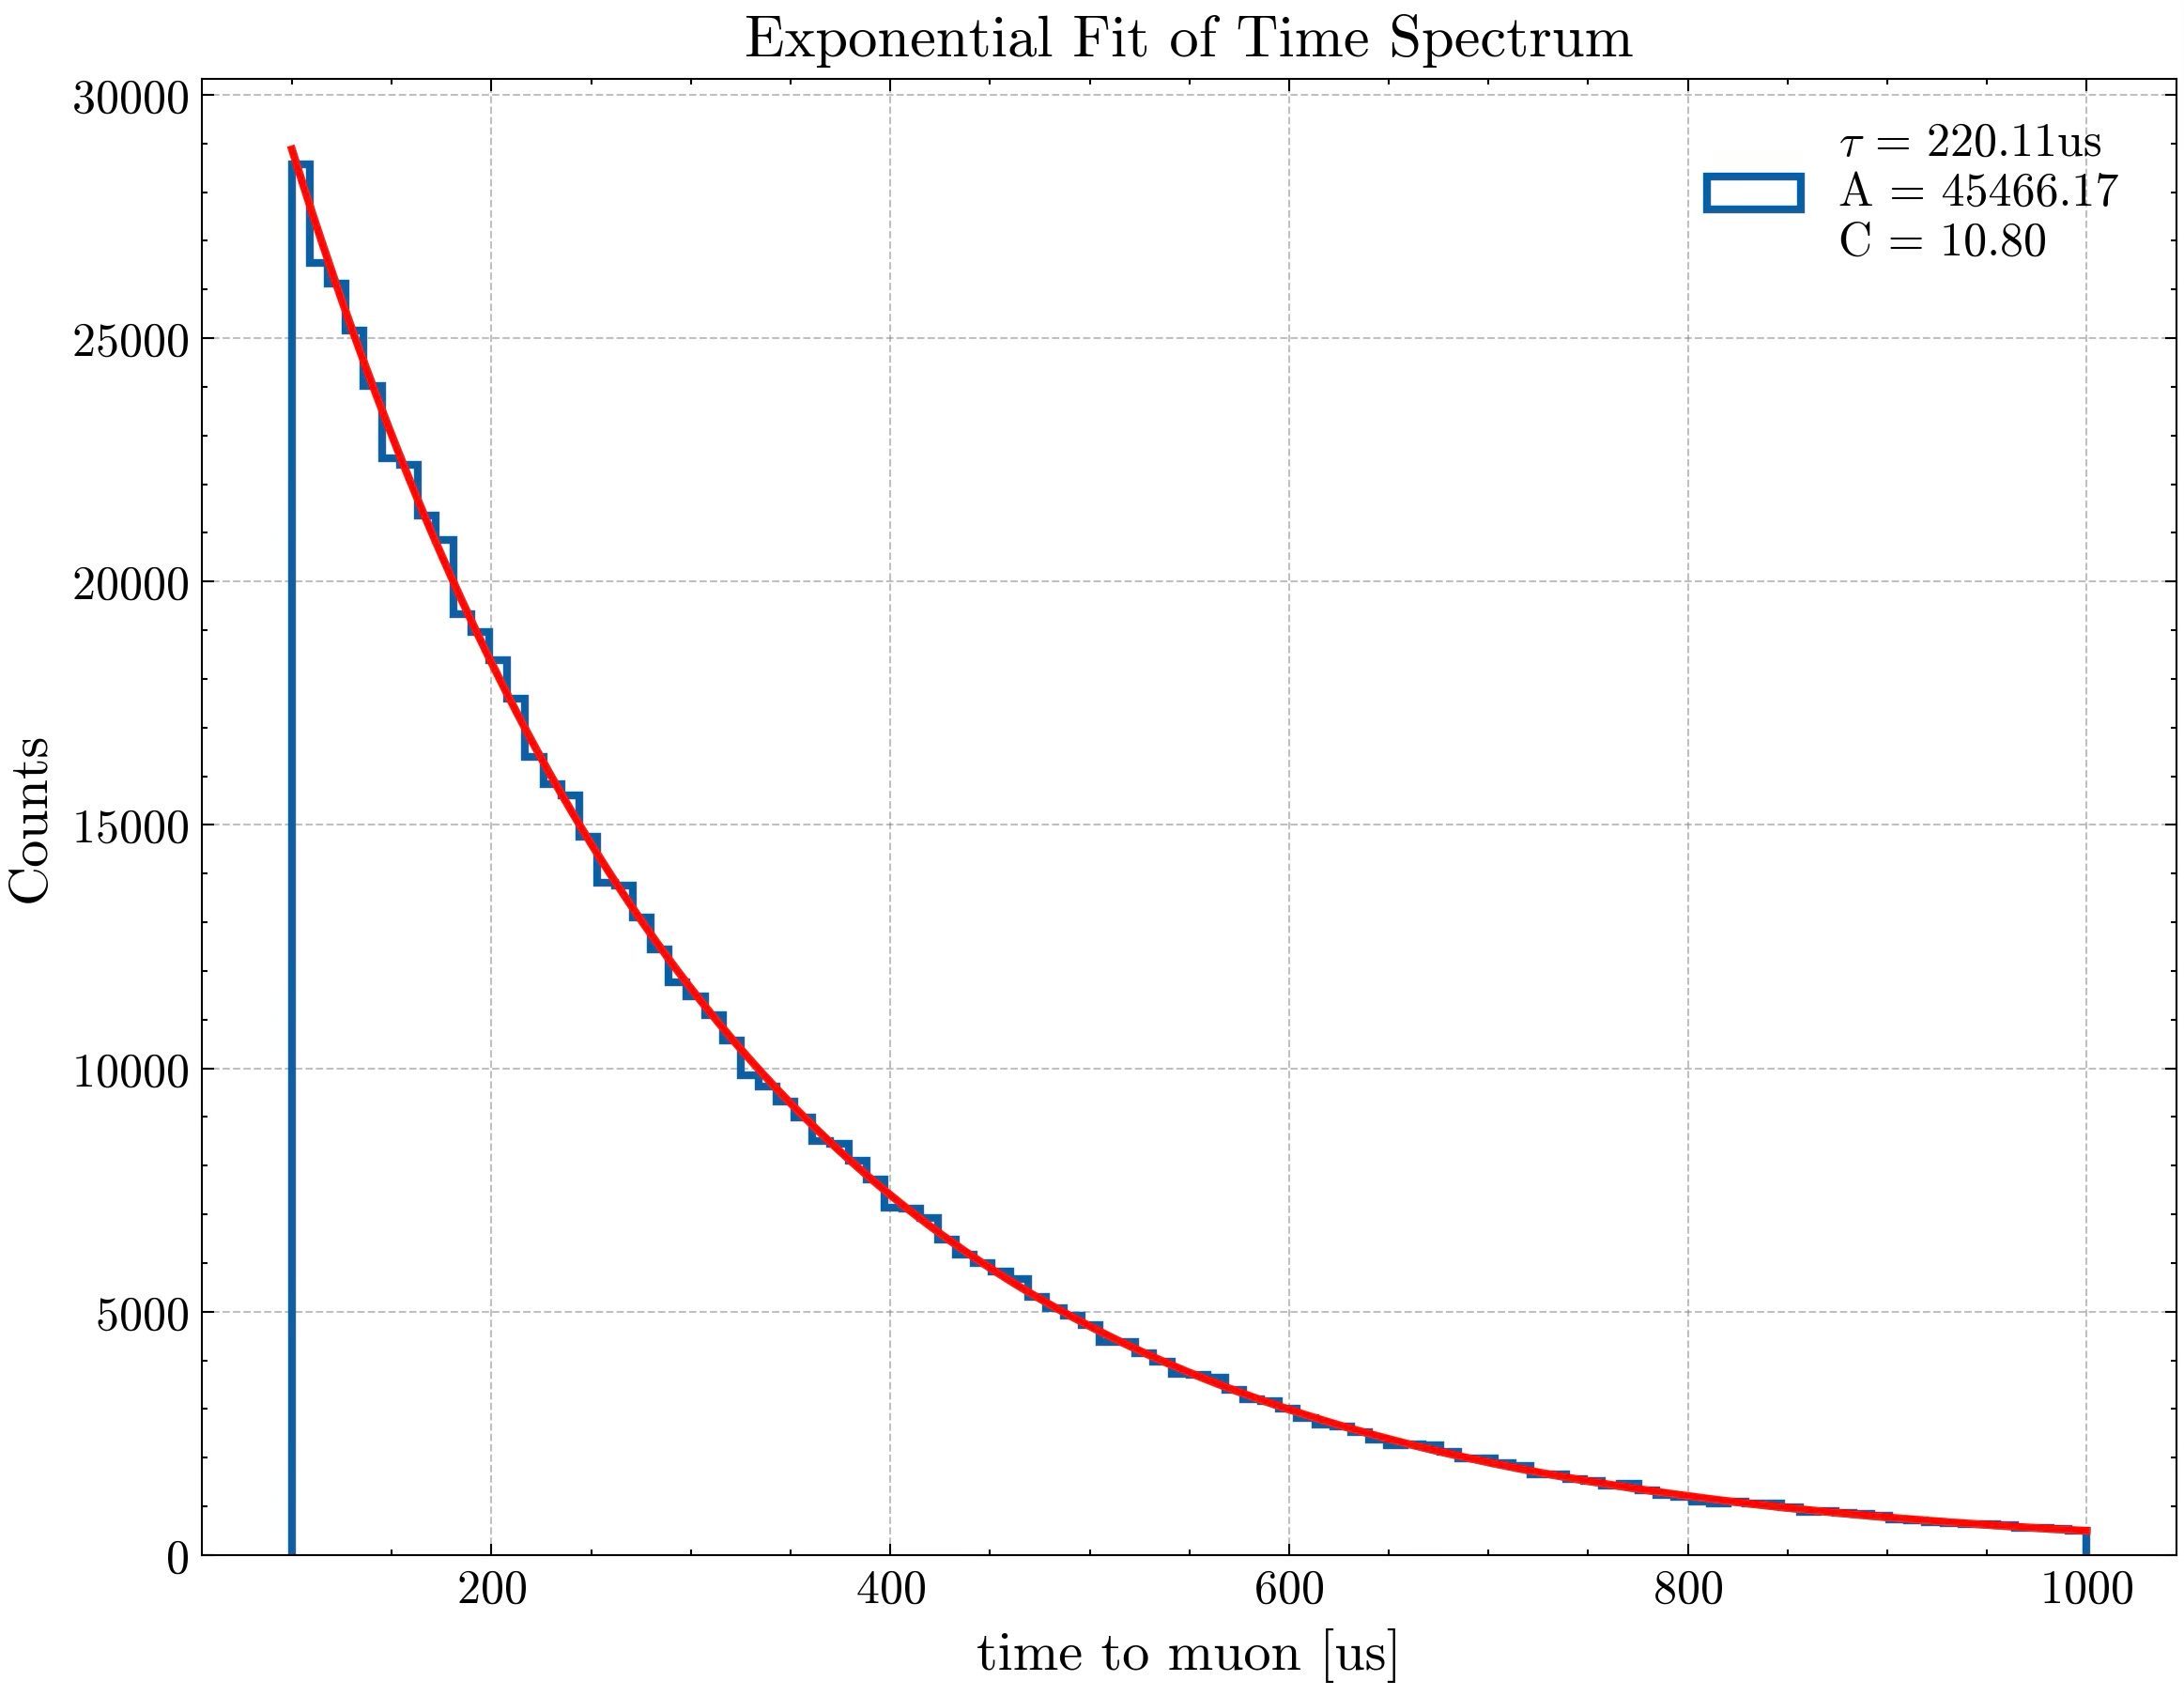
\includegraphics[width=\linewidth]{4_efficiency/SPN_dtFit.png}
        \caption{}
    \label{fig:spnDtFit}
    \end{subfigure}
    \caption{Fits to the energy spectrum~(a) and time distribution~(b) of the spallation neutron enriched sample, yielding a reconstructed energy peak at 2.26~MeV and a characteristic capture time of 220~$\mu$s for spallation neutrons captured by hydrogen.}
    \label{fig:spnFit}
\end{figure}


\subsubsection{Energy scale}
\label{subsec:energy_scale}

The accuracy of the energy reconstruction, known as the energy scale, is a critical input for precision physics measurements in JUNO, particularly for neutrino oscillation analyses. This section details the methodology for establishing, monitoring, and evaluating the systematic uncertainty of the energy scale using the P25C OMILRec dataset.

The energy scale is primarily monitored and corrected using two independent, high-statistics neutron samples: the AmC calibration source (via nH capture) and SPN. The AmC source provides precise, point-like calibrations, while the naturally occurring SPN events enable continuous, detector-wide monitoring. A significant energy drift was observed through P25C dataset. Following this shift, the method for energy drift correction transitioned from using the centrally deployed periodic AmC source to utilizing the SPN sample. The SPN-based correction accounts for the radial dependence of the energy response by calculating average correction factors within concentric spherical shells (e.g., \( R: [0.00, 10.39) \) m, \( [10.39, 13.10) \) m, etc.), providing a robust, day-by-day correction. The timeline of this transition and the evolution of the correction factors are illustrated in Fig.~\ref{fig:energy_correction_timeline}.

\begin{figure}[h!]
    \centering
    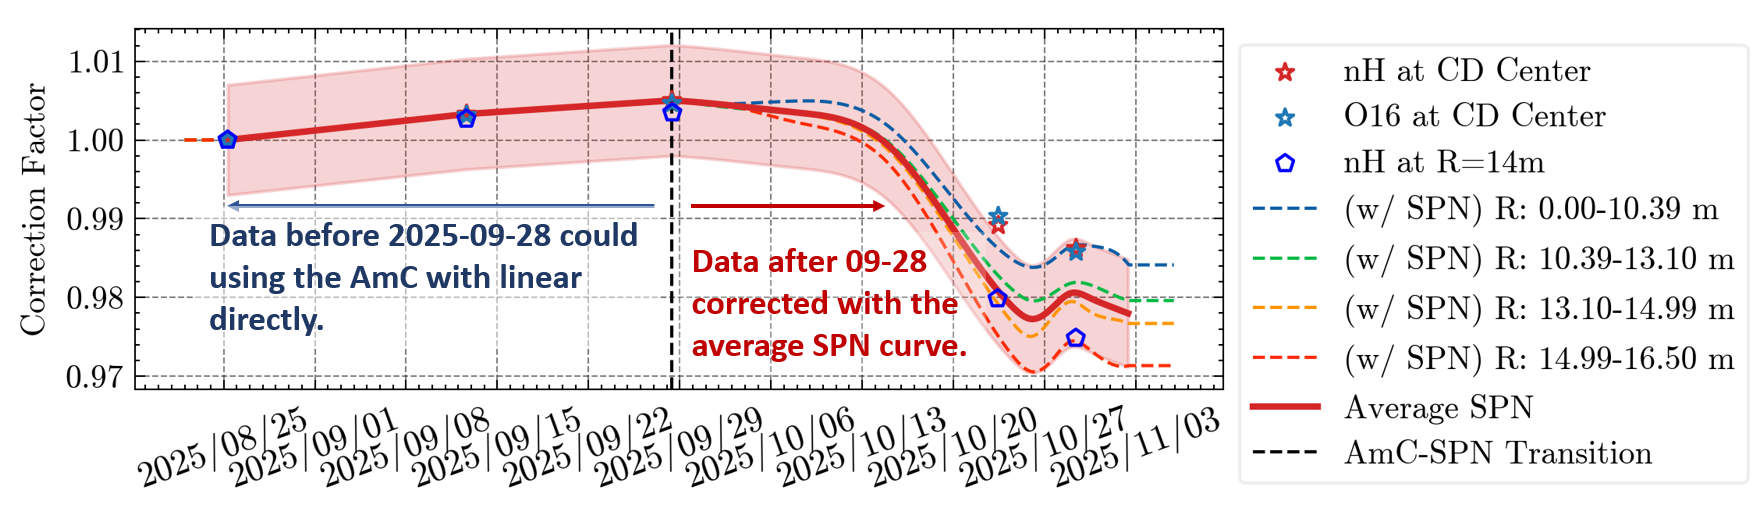
\includegraphics[width=0.9\linewidth]{4_efficiency/energy_scale_correction_timeline.png}
    \caption{
        Timeline of the energy scale correction factor. The correction methodology transitioned from using the central AmC source to a spallation neutron (SPN) based approach after September 28, 2025.
    }
    \label{fig:energy_correction_timeline}
\end{figure}

\paragraph{Assessment of Residual Temporal and Spatial Variations}

The systematic uncertainty of the energy scale is decomposed into residual temporal variation and residual detector non-uniformity. These components are constrained using full-detector samples: cosmogenic SPN and naturally occurring \( ^{214}\text{Po} \) and \( ^{210}\text{Po} \) isotopes from the \( ^{238}\text{U} \) and \( ^{232}\text{Th} \) decay chains.

The temporal stability is quantified by analyzing the daily average of the reconstructed energy \( E_{\text{rec}} \) for the \( ^{210}\text{Po} \) sample and SPN events. The observed root-mean-square (RMS) variation constrains the residual temporal instability to approximately \textbf{0.20\%}. 

To evaluate the spatial non-uniformity, the detector volume is partitioned into equal-volume boxes based on the statistics of available calibration samples. The partitioning scheme uses intervals in \( R^3 \), \( \cos\theta \), and \( \phi \) coordinates to ensure approximately equal statistics in each box. The reconstructed energy \( E_{\text{rec}} \) is calculated for each box using the \( ^{210}\text{Po} \) and SPN samples. The overall spatial variation is then determined by computing the RMS of the \( E_{\text{rec}} \) values across all boxes:

\[
\sigma_{\text{spatial}} = \sqrt{\frac{1}{N-1} \sum_{i=1}^{N} \left( E_{\text{rec}}^i - \langle E_{\text{rec}} \rangle \right)^2 }
\]

where \( N \) is the number of boxes, \( E_{\text{rec}}^i \) is the reconstructed energy in the \( i \)-th box, and \( \langle E_{\text{rec}} \rangle \) is the average reconstructed energy across all boxes. This analysis reveals a residual spatial non-uniformity of \textbf{0.45\%} within the fiducial volume. The consistency of the energy scale derived from these independent, full-volume samples validates that the temporal and spatial variations are well-understood and controlled. This analysis is summarized in Fig.~\ref{fig:energy_stability_uniformity}.

\begin{figure}[h!]
    \centering
    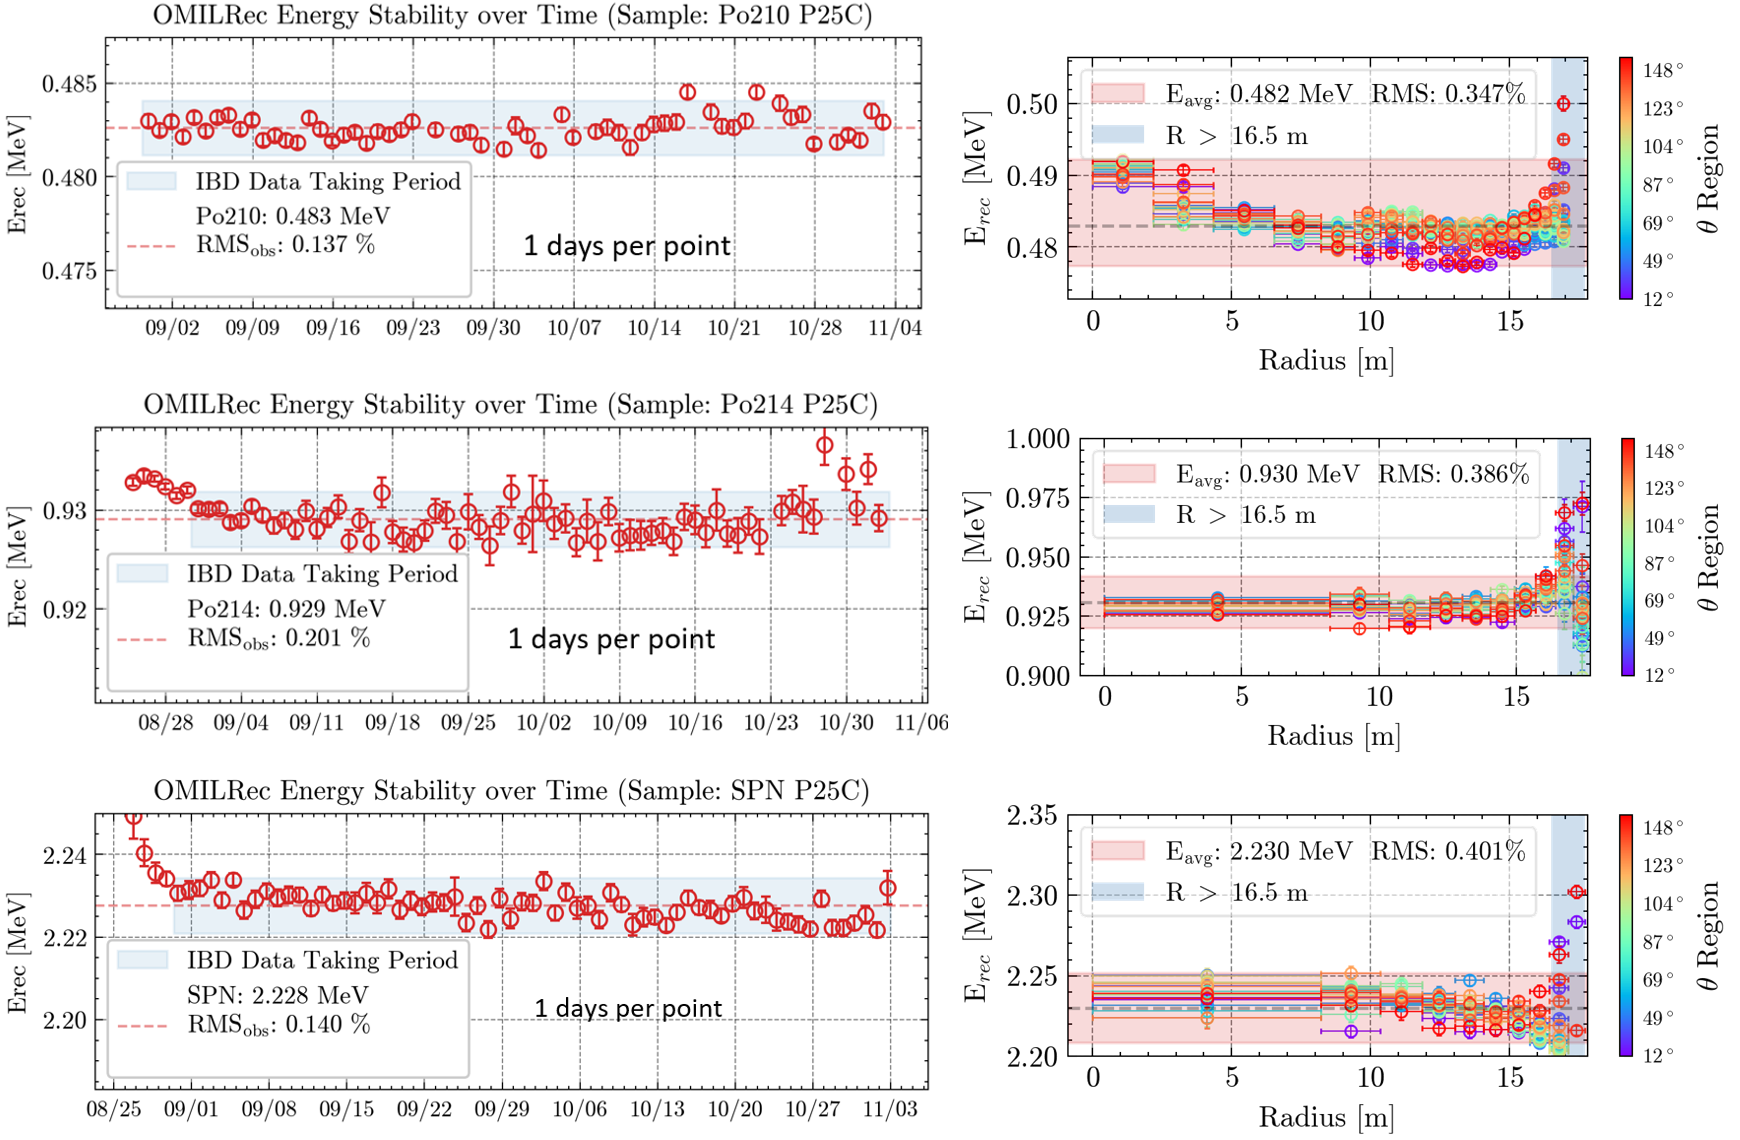
\includegraphics[width=\linewidth]{4_efficiency/energy_scale_stability_uniformity.png}
    \caption{
        Characterization of residual energy scale variations. \textbf{Left} Temporal stability of the reconstructed energy \( E_{\text{rec}} \) for the \( ^{210}\text{Po} \) sample and spallation neutrons. \textbf{Right} Spatial uniformity of \( E_{\text{rec}} \) as a function of detector radius \( R \) for the same samples in the left.
    }
    \label{fig:energy_stability_uniformity}
\end{figure}

\paragraph{Overall Systematic Uncertainty}

The overall systematic uncertainty on the energy scale is conservatively estimated by combining the residual temporal variation (\( \sigma_{\text{time}} \sim 0.20\% \)) and spatial non-uniformity (\( \sigma_{\text{spatial}} \sim 0.45\% \)) in quadrature:

\[
\sigma_{\text{total}} = \sqrt{ \sigma_{\text{time}}^2 + \sigma_{\text{spatial}}^2 }
\]

This yields a energy uncertainty of \textbf{0.50\%}. The robustness of this estimate is demonstrated by the excellent agreement among various independent calibration sources, as shown in Fig.~\ref{fig:energy_bias_uncertainty}. The energy bias \( (E_{\text{rec}} - E_0)/E_0 \) is plotted for neutrons from the AmC source, cosmogenic spallation, antineutrino candidates, \( \gamma \)-sources at fixed positions, and \( \alpha \)-decays from \( ^{214}\text{Po}/^{210}\text{Po} \). For the uniformly distributed \( ^{214}\text{Po} \) and \( ^{210}\text{Po} \) samples, which lack a defined central point, the average reconstructed energy \( \langle E \rangle \) over the detector volume is used as the reference value \( E_0 \). All measurements fall within the \textbf{±0.5\%} uncertainty band, confirming the reliability of the assigned systematic uncertainty for the energy scale in the energy region of interest for JUNO.

\begin{figure}[h!]
    \centering
    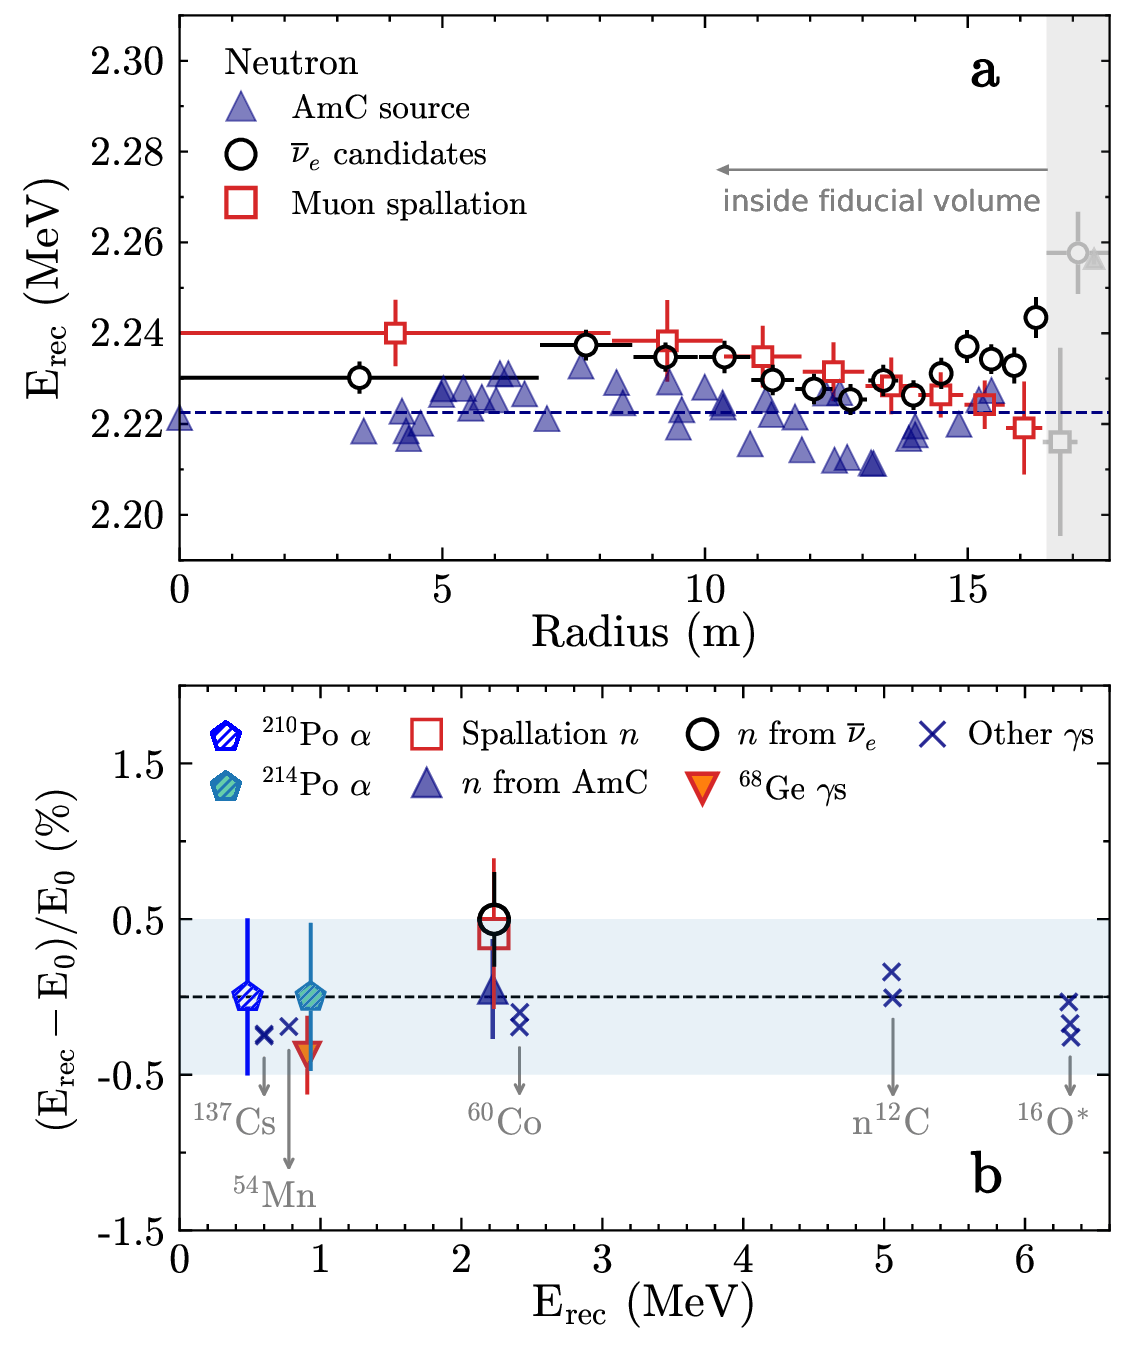
\includegraphics[width=0.8\linewidth]{4_efficiency/energy_bias_uncertainty.png}
    \caption{
        Residual energy bias and systematic uncertainty for the JUNO detector. The relative bias \( (E_{\text{rec}} - E_0)/E_0 \) is shown for various calibration sources, including neutrons (AmC, spallation, from IBD candidates), \( \gamma \)-sources, and \( \alpha \)-decays (\( ^{214}\text{Po}/^{210}\text{Po} \)). For the latter, the average reconstructed energy \( \langle E \rangle \) is used as \( E_0 \). Error bars include contributions from residual temporal and spatial variations. The shaded band represents the overall ±0.5\% systematic uncertainty assigned to the energy scale.
    }
    \label{fig:energy_bias_uncertainty}
\end{figure}

\subsubsection{Energy non-linearity}

This section introduces the modeling of the detector energy response to describe the relationship between the true energy of incident particles and the reconstructed energy. The modeling strategy mainly follows that of the Daya Bay experiment \cite{DayaBay:2019fje}. For JUNO, the non-linearity is predominantly governed by scintillation non-linearity; however, potential reconstruction-induced non-linearity require careful consideration. 

The Birks law is a semi-empirical method used to describe the quenching effect and was applied in this analysis. Several strategies are available for generating the quenching curves with different Birks'  coefficient ($k_B$), including a numerical integration method using $dE/dx$ data from ESTAR and a simulation-based approach utilizing Geant4. These two methods were respectively employed and compared. The Cherenkov contributions can also be modeled using various methods, including a Geant4-based simulation approach, a parametric function-based method, and an approach utilizing the Frank-Tamm formula. Considering the complex absorption and re-emission processes in the LS, only the shape of the Cherenkov contribution is used, and a free parameter $k_C$ is incorporated into the energy non-linearity model. Meanwhile, an additional free parameter $A$ is introduced to describe the absolute energy scale of scintillation non-linearity.


\begin{figure}[h]
  \centering
  \begin{subfigure}[t]{0.45\textwidth}
    \centering
    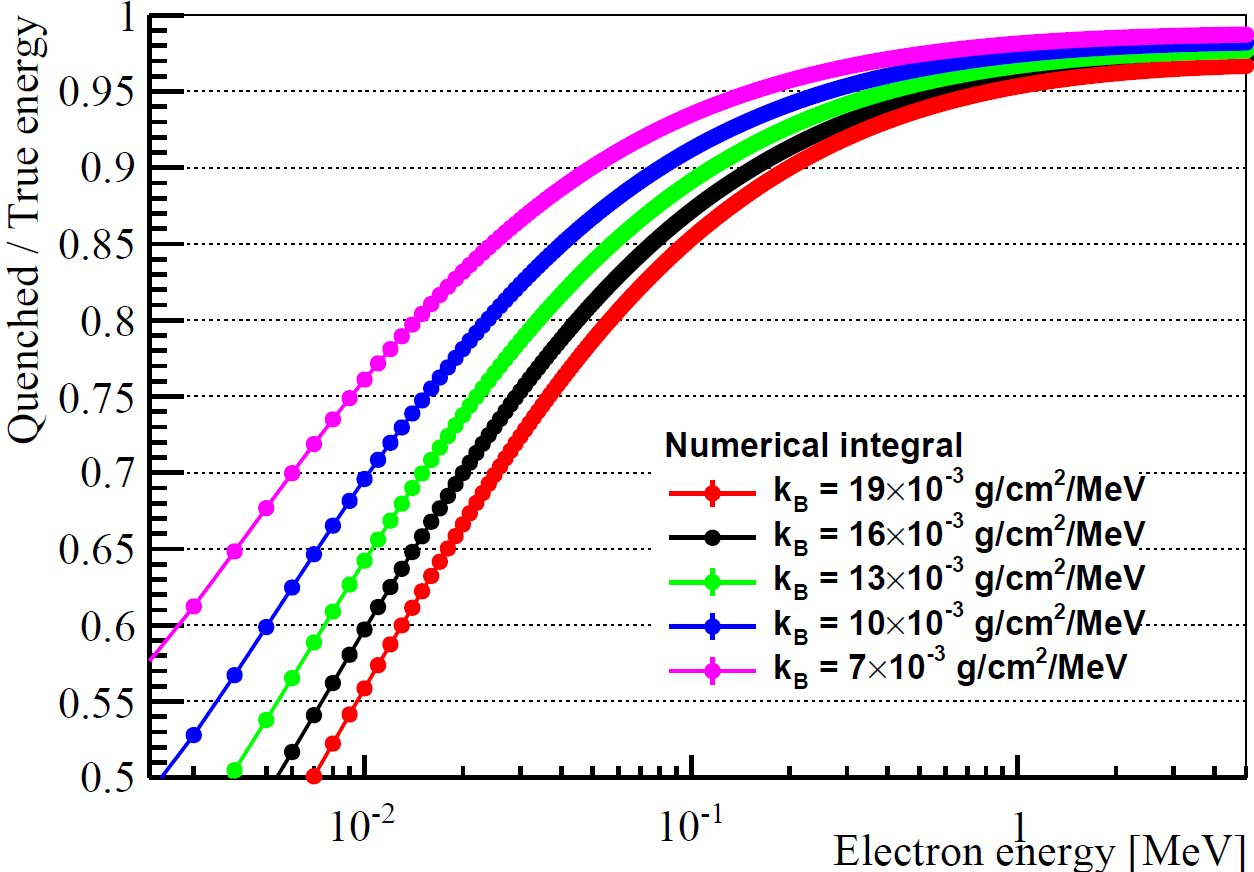
\includegraphics[width=\linewidth]{4_efficiency/quenchingCurves.png}
    \caption{}
    \label{fig:quenchingCurves}
  \end{subfigure}
  \hfill
  \begin{subfigure}[t]{0.45\textwidth}
    \centering
    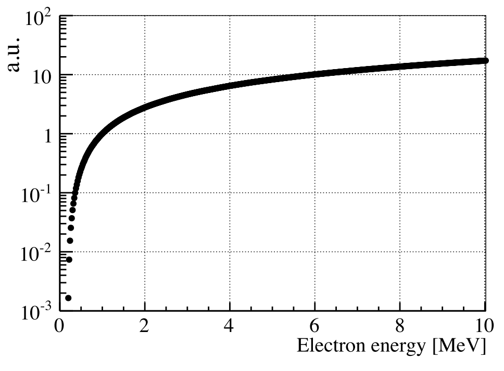
\includegraphics[width=\linewidth]{4_efficiency/CherenkovCurve.png}
    \caption{}
    \label{fig:CherenkovCurve}
  \end{subfigure}
  \caption{Examples of quenching curve and Cherenkov curve. (a) Relationship between deposited energy and visiable energy with different $k_B$ values, calculated with the numerical integration method. (b) The Cherenkov contribution to the $e^-$ kinetic energies, generated by Geant4 simulation and normalized at 1 MeV.}
\end{figure}

It is expected that minor deviations may occur in the COTI charge calculation under conditions involving multiple photoelectrons. According to current SPMT study \cite{spmt_doc_db}, the single-channel charge non-linearity of the LPMT remains below approximately 1\% over the range from 0 to 10 p.e. This non-linearity in charge reconstruction will be propagated to the energy measurement, referred to as the reconstruction non-linearity. In the analysis, it is assumed that the potential reconstruction non-linearity can be described by a gentle exponential function or a linear function, with all normalization points set at the nH peak position (2.223 MeV). For comparison, the case in which the reconstruction non-linearity is strictly zero—corresponding to perfect charge reconstruction—was also analyzed.

To constrain the model parameters and determine the energy nonlinear response, calibration is performed using data from multiple calibration sources positioned at the center of the detector and two kinds of continuous spectra from
high-purity samples ($\rm ^{12}B$ and $\rm ^{11}C$) of cosmogenic isotopes reconstructed in the FV. The former provides eight calibration points ($\rm ^{137}Cs$, $\rm ^{54}Mn$, $\rm ^{40}K$, $\rm ^{68}Ge$, $\rm nH$, $\rm ^{60}Co$, $\rm n^{12}C$, $\rm ^{16}O^{\star}$), which are detailed in Section~\ref{subsec:fv_selection}. The latter yields a continuous $\beta^{-}$ spectrum from $\rm ^{12}B$ decays and a $\beta^{+}$ spectrum from $\rm ^{11}C$ decays, with the visible energy increased by 2 $\times$ 511 keV due to annihilation gamma rays. Further details regarding the analysis of the calibration data can be found in \cite{sourceAna_doc_db} and \cite{spectrumAna_doc_db}.

All model parameters are determined through $\chi^{2}$ minimization to the combined calibration data. Considering that all the calibration sources are loaded at the center of the detector, the majority of the signals received by the PMTs are single photons. The corresponding charge reconstruction deviation can be ignored, so the reconstruction non-linearity was neglected when expecting their energy non-linearity. However, for the $^{12}$B sample which is uniformly distributed over the entire detector, the influence of potential reconstruction non-linearity was considered. The best-fit results to the mono-energetic peaks from gamma calibration sources and the continuous energy spectra from cosmogenic isotopes, as well as the predicted electron and positron non-linearities, are shown in Fig.~\ref{fig:Energy-nonlinearity}. An overall non-linearity uncertainty of 1\% is achieved for positron.

\begin{figure}[h!]
    \centering
    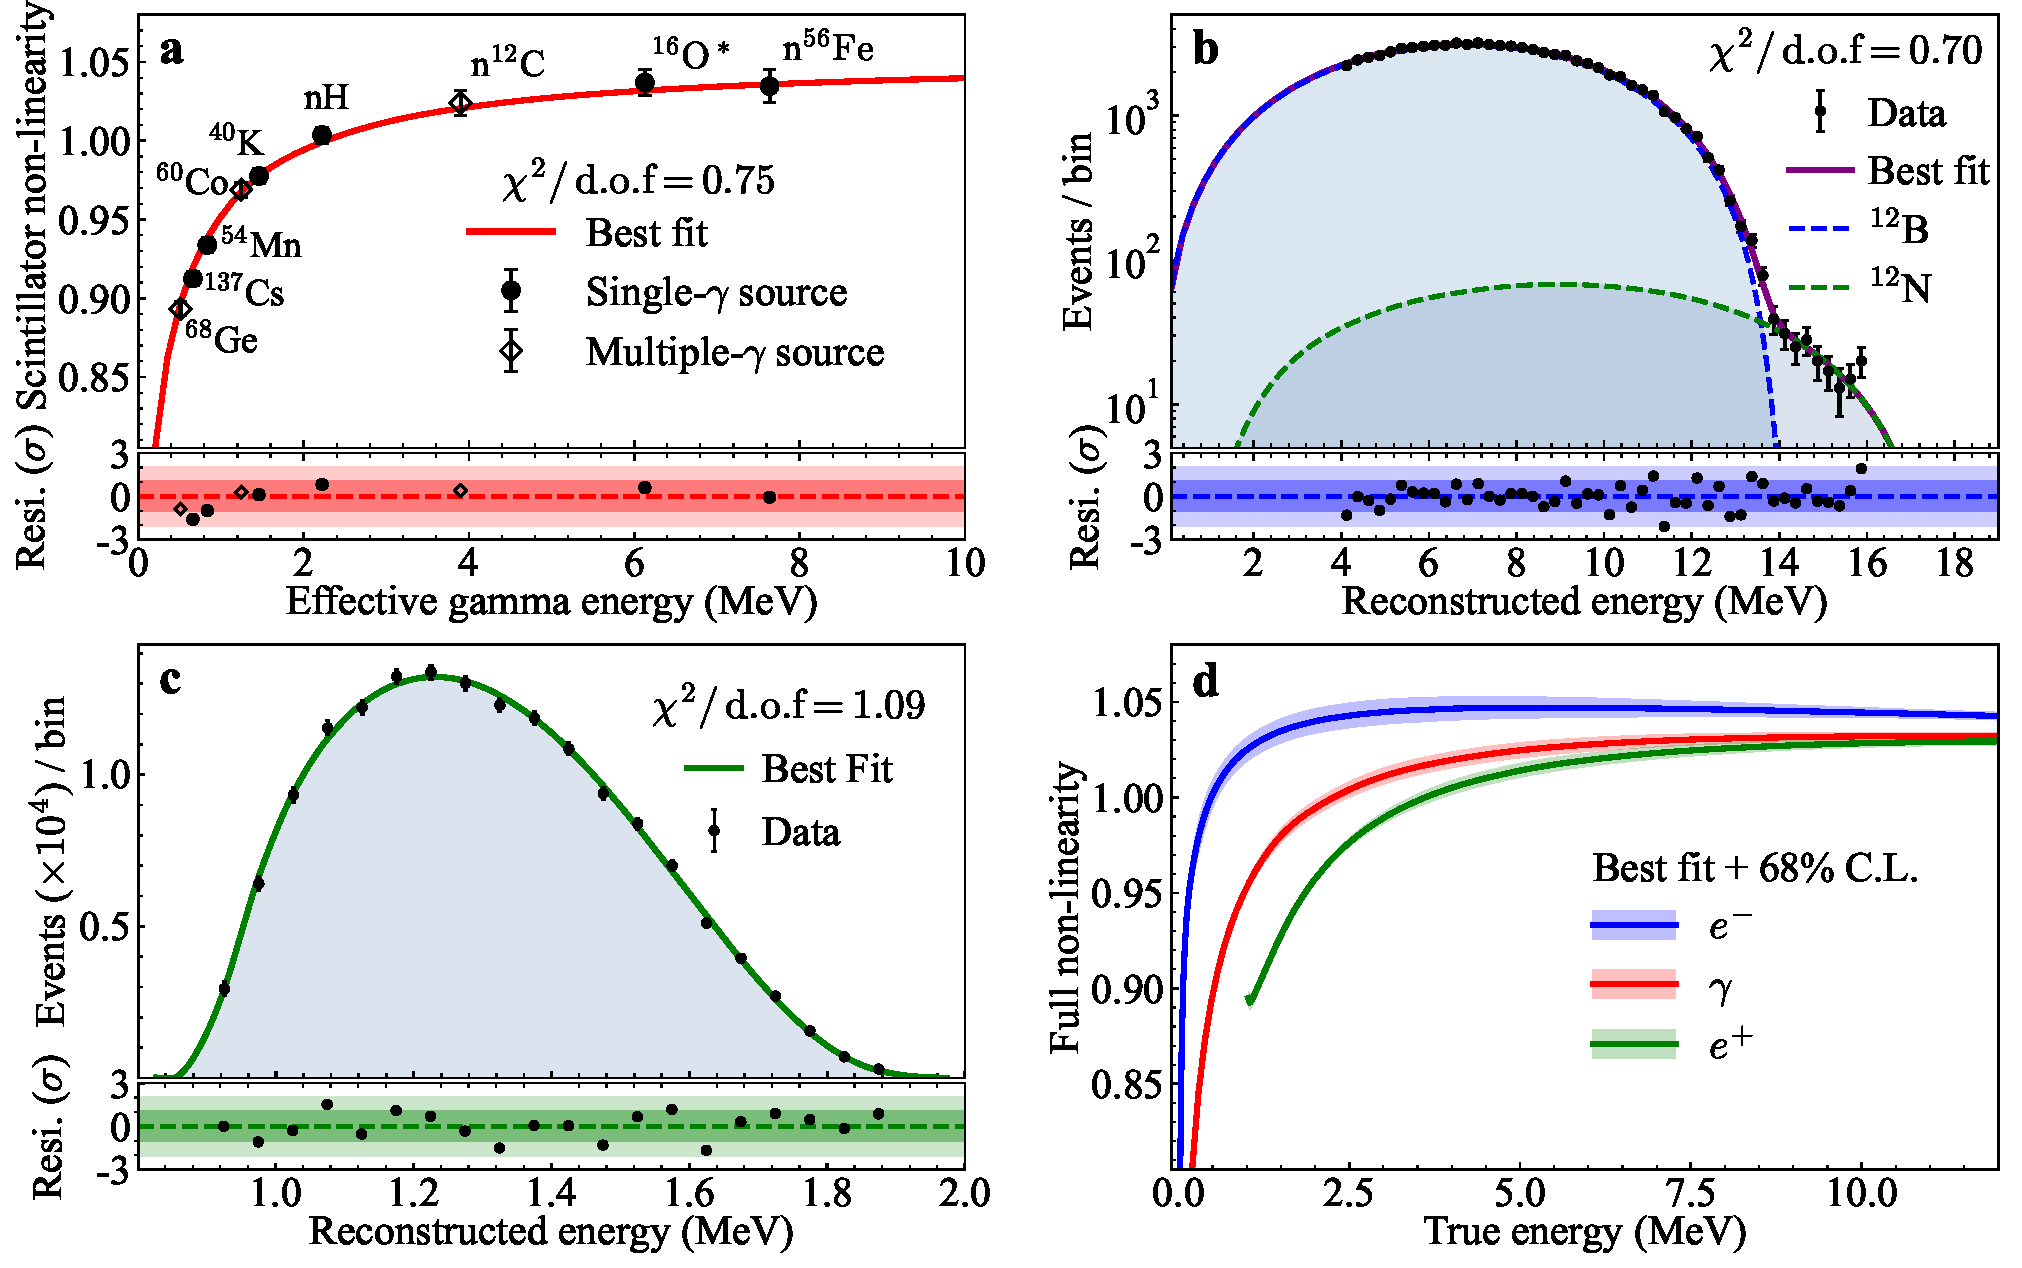
\includegraphics[width=0.9\linewidth]{4_efficiency/Energy-nonlinearity-groupA-Plots-fromYongbo-V15.pdf}
    \caption{Energy scale non-linearity calibration. \textbf{a}, Scintillator non-ninearity from $\gamma$ calibration sources deployed at the detector's center: single-$\gamma$ sources (solid circle), multiple-$\gamma$ sources (hollow rhombus), and the best-fit curve (red). \textbf{b}, Measured cosmogenic $^{12}$B $\beta^{-}$ spectrum (points) compared to prediction (blue line), with a best-fit $^{12}$N component (green dashed line)of 2.7\% identified via its high-energy shoulder. \textbf{c}, Measured $^{11}$C $\beta^{+}$ spectrum (points) and the best-fit model (green line). \textbf{d}, Non-linearity response model for electrons (blue), $\gamma$'s (red), and positrons (green).}
    \label{fig:Energy-nonlinearity}
\end{figure}


In addition, more tests and examinations were conducted, including the use of $^{12}$B samples from different selection strategies and different vertices, etc. A comparison of the non-linearity fits performed under two assumptions—no reconstruction non-linearity and the presence of reconstruction non-linearity (with pull parameter constrained)—shows that the resulting positron non-linearity curves do not differ significantly, with a discrepancy of approximately 0.2\% at 12 MeV. On the other hand, the de-excitation $\gamma$ from neutron absorption on Fe (n$^{56}$Fe) was used for additional validation. It was observed that including the n$^{56}$Fe calibration point in the fit leads to a change of less than 0.02\% in the positron non-linearity, as the $^{12}$B sample provides dominant constraints in the high-energy region. More details and comparison results can be found in \cite{ENL_check_doc_db}. 

\subsubsection{Energy resolution}
\label{subsubsection:EReso}
The energy resolution of the JUNO detector is a fundamental performance parameter that directly impacts the precision of neutrino oscillation measurements. Accurate characterization of the energy resolution is achieved through careful fitting of gamma source spectra. The fitting of gamma source energy spectra provides essential information about the detector's response function, statistical fluctuations, and systematic effects. The quality of these fits determines the reliability of the extracted resolution parameters, which are crucial inputs for the ABC model and subsequent physics analyses.


The energy resolution of the JUNO detector is parameterized using the ABC model, which describes the relative energy resolution $\sigma_E/E$ as a function of visible energy $E$:

\begin{equation}
\frac{\sigma_E}{E} = \sqrt{ \left(\frac{a}{\sqrt{E}}\right)^2 + b^2 + \left(\frac{c}{E}\right)^2 }
\label{eq:abc_model}
\end{equation}

where:
\begin{itemize}
    \item $a$ represents the statistical term related to photon statistics,
    \item $b$ is the constant term accounting for detector non-uniformity and systematic effects,
    \item $c$ is the noise term from electronics and dark noise.
\end{itemize}

This model captures the three dominant contributions to the energy resolution and provides a comprehensive description of the detector's energy response across the full energy range.

It is important to note that the energy resolution in JUNO exhibits particle dependence, as demonstrated in previous studies (e.g., Miao Yu et al.). The resolution for different particle types (electrons, positrons, gammas, etc.) can vary due to differences in energy deposition mechanisms, light yield, and ionization quenching effects. However, due to time constraints and the complexity of implementing particle-dependent resolution models, the current analysis for the P25C dataset utilizes the gamma resolution model as a conservative and standardized approach. This simplification provides a robust baseline for the energy resolution characterization while acknowledging that future analyses may incorporate particle-dependent corrections for improved precision.

\begin{figure}[h!]
    \centering
    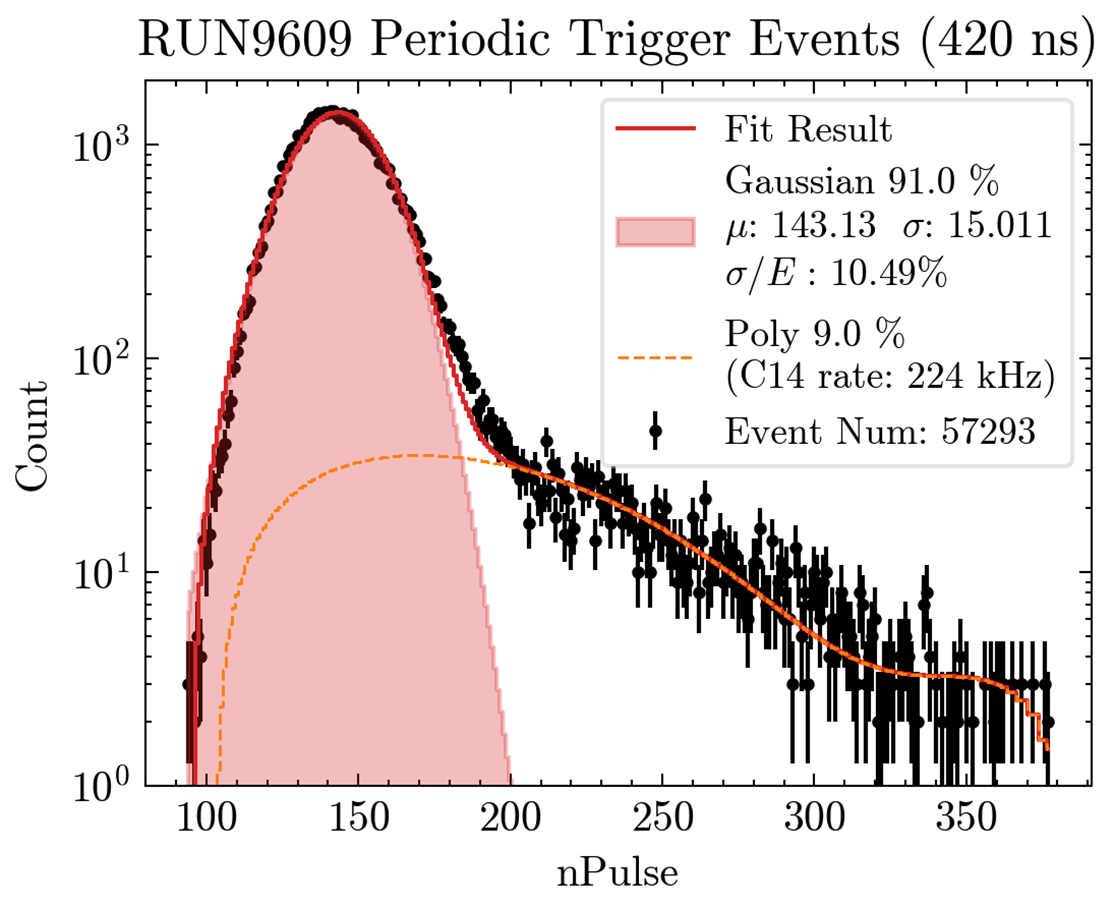
\includegraphics[width=0.8\textwidth]{4_efficiency/periodic_trigger_spectrum.png}
    \caption{Periodic trigger events nPulse spectrum of RUN9609 in 420 ns time window.}
    \label{fig:periodic_trigger}
\end{figure}

The presence of this $^{14}\text{C}$ pile-up tail distorts the energy spectrum of calibration sources. In an ideal, noise-free detector, the response to a mono-energetic gamma would be a near-Gaussian peak. However, the $^{14}\text{C}$ pile-up, by randomly adding low-energy deposits to physical events, broadens and asymmetrically skews this peak as shown in Fig.~\ref{fig:periodic_trigger}. Since a dedicated algorithm for identifying and subtracting $^{14}\text{C}$ pile-up events has not been applied to the P25C dataset, a critical question arises: how does the choice of fitting model (with or without explicit $^{14}\text{C}$ consideration) affect the extracted energy resolution? The following sections will detail and compare these two fitting strategies to quantify this effect.


\paragraph{Fitting Models Without $^{14}\text{C}$ Consideration}
For the majority of calibration sources, two simplified fitting approaches are employed when ignoring $^{14}\text{C}$ effects:
\begin{enumerate}
    \item \textbf{Purely Empirical Formula}: A Gaussian peak plus polynomial background, as shown for $^{137}\text{Cs}$ in Fig.~\ref{fig:cs137_wo_c14}(left).
    \item \textbf{MC-Based Spectrum Fitting for $^{68}$Ge}: Using MC simulations to generate template spectra for fitting, as shown in in Fig.~\ref{fig:cs137_wo_c14}(right).
\end{enumerate}


\begin{figure}[h!]
    \centering
    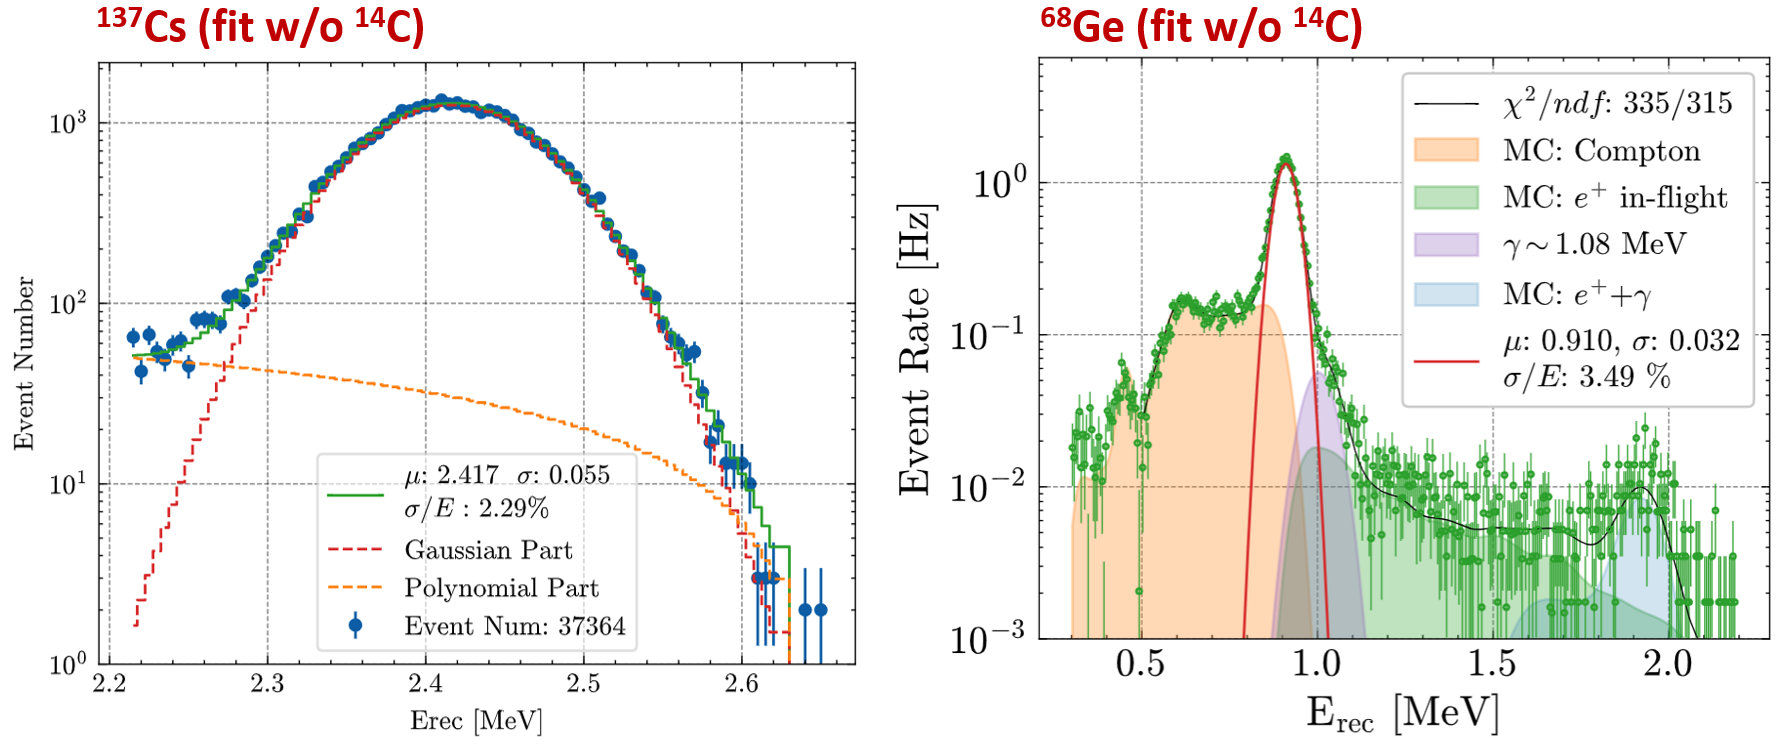
\includegraphics[width=0.8\textwidth]{4_efficiency/Cs137_wo_c14.png}
    \caption{\textbf{Left}: $^{60}\text{Co}$ energy spectrum fitted without $^{14}\text{C}$ consideration. The 2.506 MeV $\gamma$ peak is modeled as a Gaussian plus a polynomial background.\textbf{Right}: MC-based fitting result of $^{68}$Ge}
    \label{fig:cs137_wo_c14}
\end{figure}

\paragraph{Fitting Model with $^{14}\text{C}$ Consideration}
To properly account for $^{14}\text{C}$ effects, we developed a comprehensive fitting framework that incorporates probability weights. The complete model for $^{137}$Cs is formulated as:

\begin{equation}
\begin{aligned}
F_{\text{total}}(E) = & (1 - p - p^{2}) \cdot \left[ A_{\text{FEP}} \cdot f_{\text{FEP}}(E; \mu, \sigma) + A_{\text{Compton}} \cdot f_{\text{Compton}}(E) \right] \\
& + p \cdot F_{\text{1-pile}}(E) + p^{2} \cdot F_{\text{2-pile}}(E)
\end{aligned}
\label{eq:enhanced_fitting_model}
\end{equation}

where:
\begin{itemize}
    \item $A_{\text{FEP}}$ and $A_{\text{Compton}}$ are the amplitude factors for the full-energy peak and Compton background components,
    \item $f_{\text{FEP}}(E; \mu, \sigma)$ is the full-energy peak distribution, modeled as a Gaussian,
    \item $f_{\text{Compton}}(E)$ is the Compton background distribution obtained from MC simulations,
    \item $p$ represent the probabilities of $^{14}\text{C}$ pile-up events, with $(1 - p - p^{2})$ being the probability of no pile-up,
    \item $F_{\text{1-pile}}(E)$ and $F_{\text{2-pile}}(E)$ are the single and double pile-up distributions.
\end{itemize}

The pile-up terms are explicitly defined as convolution operations:

\begin{equation}
\begin{aligned}
F_{\text{1-pile}}(E) &= \left[ A_{\text{FEP}} \cdot f_{\text{FEP}}(E; \mu, \sigma) + A_{\text{Compton}} \cdot f_{\text{Compton}}(E) \right] \ast f_{\text{$^{14}$C}}(E) \\
F_{\text{2-pile}}(E) &= F_{\text{1-pile}}(E) \ast f_{\text{$^{14}$C}}(E)
\end{aligned}
\label{eq:convolution_definitions}
\end{equation}



where $\ast$ denotes the convolution operation, and $f_{\text{$^{14}$C}}(E)$ represents the $^{14}\text{C}$ Qedep energy spectrum. The energy resolution term $\sigma(E)$ used in the Gaussian components is determined by the ABC model mentioned before. Fig.~\ref{fig:with_c14_fits} shows representative fitting results with $^{14}\text{C}$ consideration for multiple sources.

\begin{figure}[h!]
    \centering
    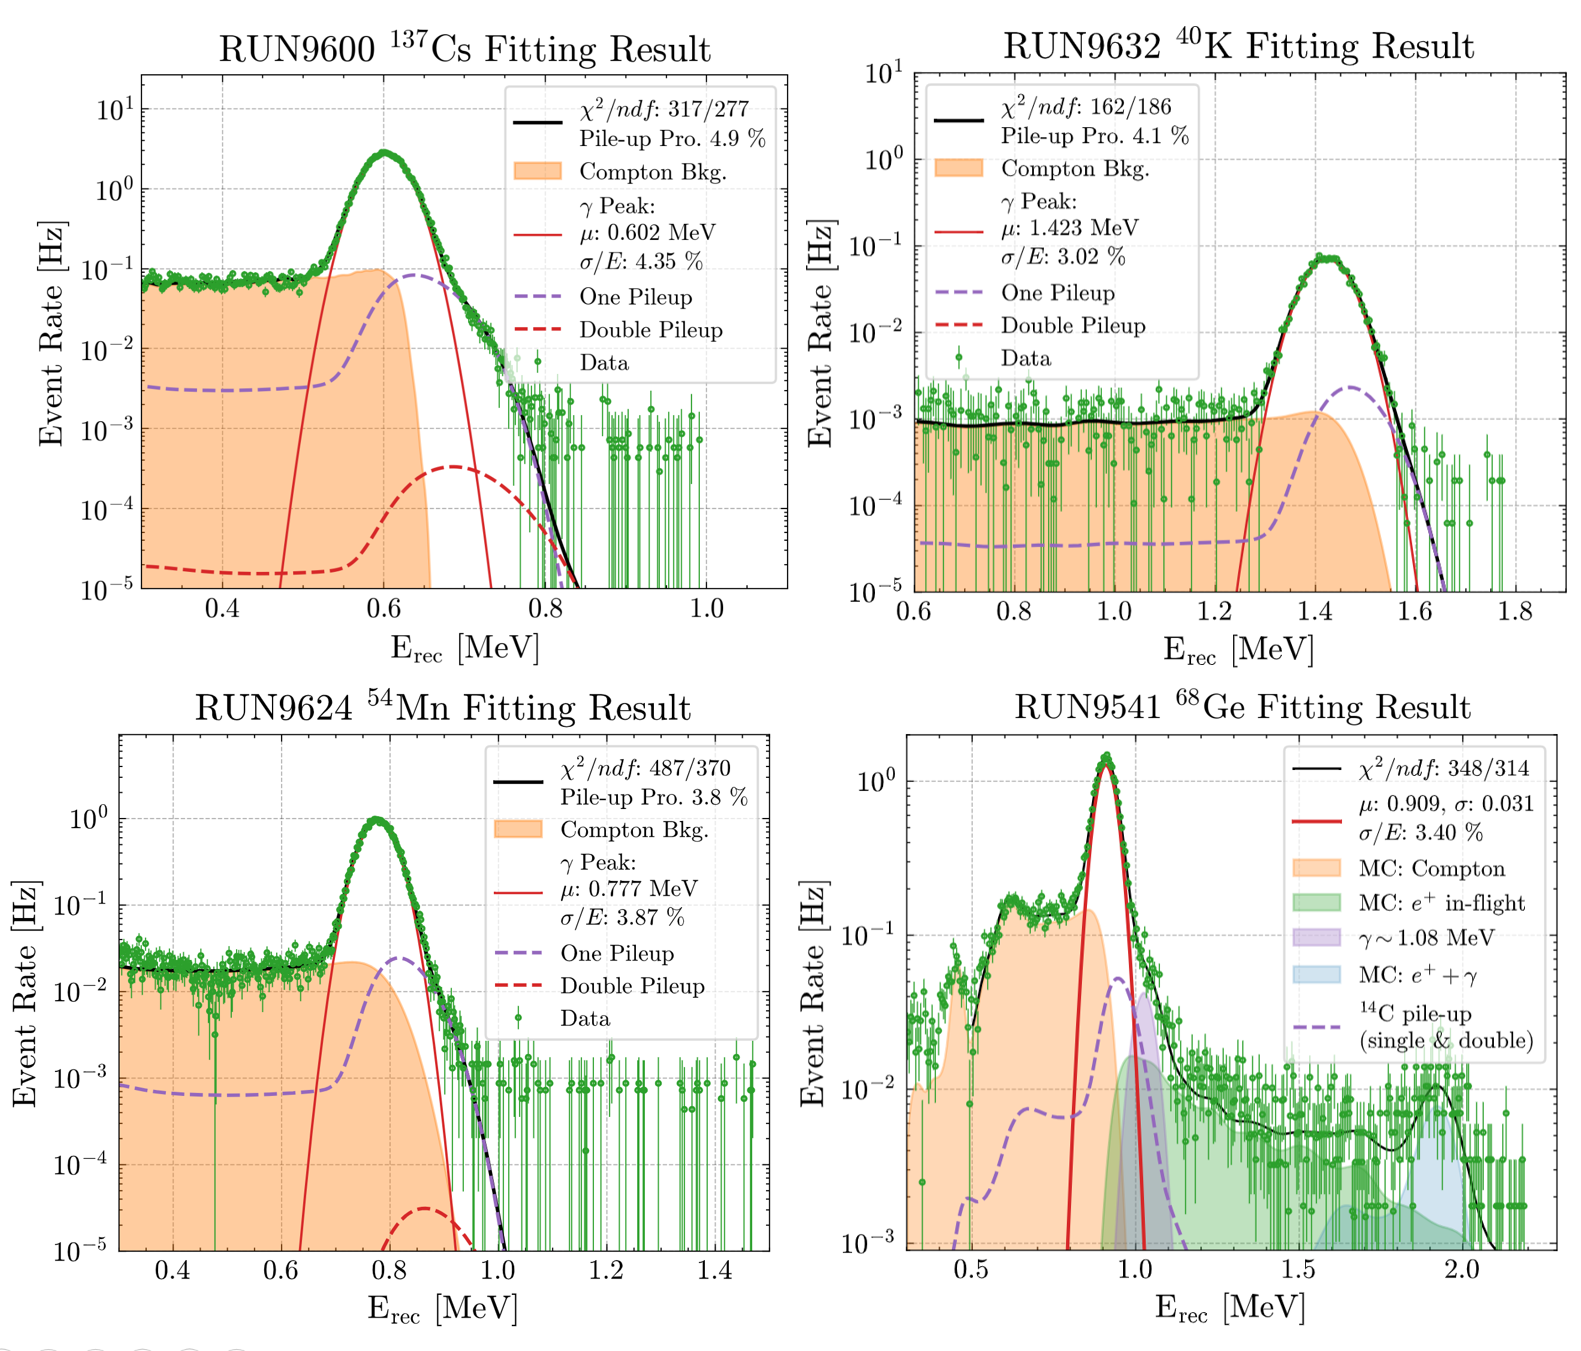
\includegraphics[width=\textwidth]{4_efficiency/with_c14_fits.png}
    \caption{Energy spectrum fits with $^{14}\text{C}$ consideration for multiple sources. Each panel shows: data (green points), total fit (black line), Compton background (orange fill), full-energy peak (red line), single pile-up (purple dashed), and double pile-up (red dashed). Fitting parameters including $\chi^2/\text{ndf}$ and pile-up probability are indicated.}
    \label{fig:with_c14_fits}
\end{figure}

Table~\ref{tab:resolution_results} summarizes the energy resolution measurements for all calibration sources, comparing results obtained with and without $^{14}\text{C}$ consideration in the fitting model.

\begin{table}[h!]
\centering
\caption{Energy resolution measurements for calibration sources. Results are shown for both fitting approaches: without $^{14}\text{C}$ consideration (w/o $^{14}\text{C}$) and with $^{14}\text{C}$ consideration (w/ $^{14}\text{C}$).}
\label{tab:resolution_results}
\resizebox{\linewidth}{!}{
\begin{tabular}{lcccc}
\toprule
\textbf{Source} & \textbf{$\text{E}_{\text{rec}}$ (w/o $^{14}\text{C}$) [MeV]} & \textbf{$\text{E}_{\text{rec}}$ (w/ $^{14}\text{C}$) [MeV]} & \textbf{Resolution (w/o $^{14}\text{C}$) [\%]} & \textbf{Resolution (w/ $^{14}\text{C}$) [\%]} \\
\midrule
$^{137}\text{Cs}$ & 0.602 & 0.602 & 4.449 & 4.349 \\
$^{54}\text{Mn}$ & 0.777 & 0.777 & 3.958 & 3.870 \\
$^{68}\text{Ge}$ & 0.910 & 0.909 & 3.526 & 3.404 \\
$^{40}\text{K}$ & 1.423 & 1.423 & 3.066 & 3.019 \\
nH & 2.221 & 2.221 & 2.576 & --- \\
$^{60}\text{Co}$ & 2.417 & 2.419 & 2.291 & 2.306 \\
nC & 5.028 & 5.028 & 2.219 & --- \\
$^{16}\text{O}$ & 6.303 & 6.303 & 1.642 & --- \\
\bottomrule
\end{tabular}
}
\end{table}

\begin{itemize}
    \item The reconstructed energies are remarkably consistent between the two fitting approaches, with differences typically less than 0.1\%.
    \item Energy resolution shows the expected improvement with increasing energy, from 4.449\% at 0.602 MeV ($^{137}\text{Cs}$) to 1.642\% at 6.303 MeV ($^{16}\text{O}$).
    \item For nH, nC, and $^{16}\text{O}$ sources, $^{14}\text{C}$-aware fitting models are not yet implemented, as indicated by the missing values in the table.
\end{itemize}

Despite the availability of the advanced $^{14}\text{C}$-aware fitting model, for the P25 dataset analysis, we have chosen to use the simplified fitting approach without explicit $^{14}\text{C}$ consideration. The Gaussian-only fit, while underestimating the true complexity, provides results that are closer to the expected physical values than the preliminary $^{14}\text{C}$-aware fits. Table~\ref{tab:abc_params_simple} shows the fitting result of the abc parameter for the energy resolution curve.

\begin{table}[h!]
\centering
\caption{ABC model parameters. Values are given as [parameter $\pm$ error].}
\label{tab:abc_params_simple}
\begin{tabular}{ccc}
\toprule
\textbf{Parameter} & \textbf{Value} \\
\midrule
$a$ (\%) & $3.310 \pm 0.016$\\
$b$ (\%) & $1.280 \pm 0.038$\\
$c$ ((\%) & $0.0014 \pm 0.3041$\\
\bottomrule
\end{tabular}
\end{table}

\paragraph{Data-MC Comparison and Residual Resolution Understanding}
The energy resolution obtained from the $^{14}\text{C}$-unaware fitting of calibration data is systematically compared with the predictions from full detector simulations. This comparison reveals a significant and energy-dependent discrepancy between the measured and simulated resolutions. As shown in the top panel of Fig.~\ref{fig:data_mc_comparison}, the relative energy resolution $\sigma/E_{\text{rec}}$ for sources at the detector center (using OMILRec reconstruction) is plotted against the reconstructed energy $E_{\text{rec}}$. The data points (DetSim Data) include both single-$\gamma$ and multi-$\gamma$ sources, while the dashed curve represents the fit considering only the single-$\gamma$ component. The clear separation between the data and the simulation curve quantifies the excess resolution observed in the experiment.

The magnitude of this discrepancy is quantified by the residual standard deviation $\sigma_{\text{res}}$, defined as the quadrature difference between the measured and simulated energy widths:
$$
\sigma_{\text{res}}(E) = \sqrt{ \sigma_{\text{Data}}^2(E) - \sigma_{\text{MC}}^2(E) }
$$
where $\sigma_{\text{Data}}(E)$ and $\sigma_{\text{MC}}(E)$ are the absolute energy standard deviations ($\sigma = (\sigma/E) \times E$) from the experimental data and MC simulation, respectively. The bottom panel of Fig.~\ref{fig:data_mc_comparison} plots $\sigma_{\text{res}}$ in keV as a function of $E_{\text{rec}}$. A key observation is that the residual $\sigma_{\text{res}}$ is consistently greater than 15 keV across the entire energy range studied, indicating a significant contribution from effects not fully captured by the current detector simulation. Furthermore, $\sigma_{\text{res}}$ exhibits a positive correlation with energy, suggesting that the underlying systematic effects have a non-stochastic, energy-dependent component.

\begin{figure}[h!]
    \centering
    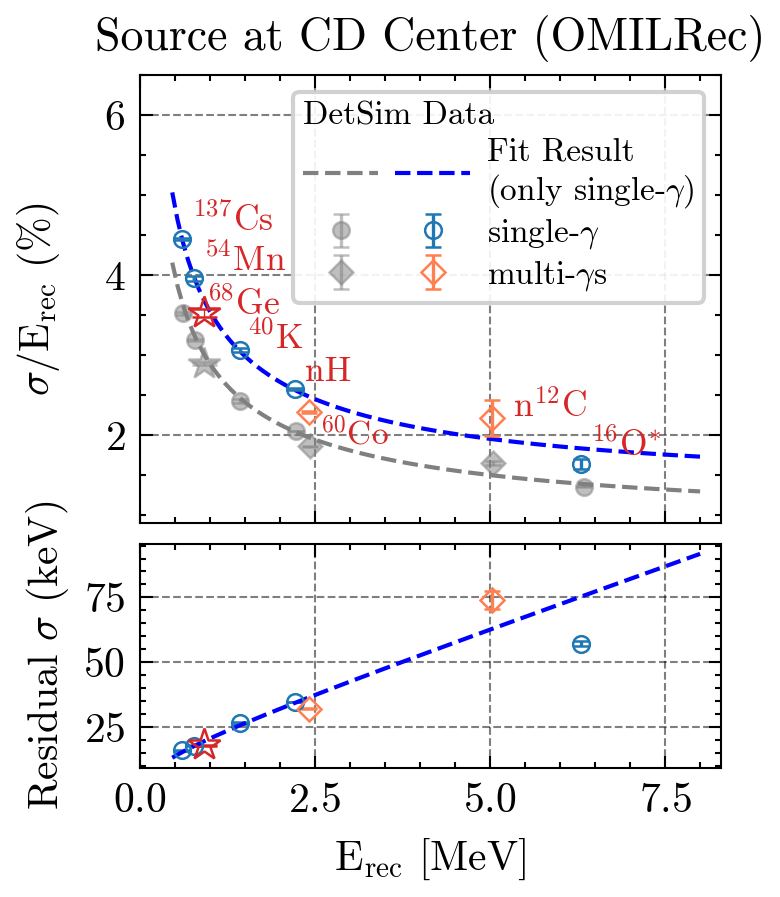
\includegraphics[width=0.85\textwidth]{4_efficiency/data_mc_resolution_center.png}
    \caption{Comparison of energy resolution between experimental data and detector simulation for sources at the detector center (OMILRec). \textbf{Top:} Relative energy resolution $\sigma/E_{\text{rec}}$ versus $E_{\text{rec}}$. Data points include single-$\gamma$ (blue circles) and multi-$\gamma$ sources (orange diamonds and red stars). The dashed line is a fit to the single-$\gamma$ simulation data. \textbf{Bottom:} Residual standard deviation $\sigma_{\text{res}} = \sqrt{\sigma_{\text{Data}}^2 - \sigma_{\text{MC}}^2}$ in keV. The residual is consistently above 15 keV and shows a positive trend with energy.}
    \label{fig:data_mc_comparison}
\end{figure}

\paragraph{Decomposition of the Residual Resolution}
To identify the physical origins of the excess resolution, a decomposition of $\sigma_{\text{res}}$ is performed. The methodology follows the framework established in previous CPC studies, where the total resolution is expressed as the quadrature sum of contributions from several independent effects. The decomposition formula is:
$$
\sigma_{\text{res}}^2 = \sigma_{\text{Vertex}}^2 + \sigma_{\text{Waveform}}^2 + \sigma_{\text{sPE Charge}}^2 + \sigma_{\text{Dark Noise}}^2 + \sigma_{\text{Other}}^2
$$
The contribution from Dark Noise ($\sigma_{\text{Dark Noise}}$) is not taken directly from simulation but is instead quantified using a toy MC method based on the high-statistics periodic trigger data as shown in Fig.~\ref{fig:periodic_trigger}, providing a more realistic estimate of its impact.

Fig.~\ref{fig:residual_decomposition} presents the result of this subtraction analysis. The black solid line represents the total $\sigma_{\text{res}}$. Starting from this total, the contributions from four key effects are sequentially subtracted in quadrature, following the order: Dark Noise, single Photoelectron (sPE) charge smear, waveform reconstruction inaccuracy, and vertex reconstruction uncertainty. The area between successive curves, filled with color, visually represents the magnitude of each contribution. The analysis indicates that the low-energy region ($E_{\text{rec}} < 1$ MeV) is dominated by the combined effects of Dark Noise and sPE charge smearing, which is well understood. However, the significant and increasing residual contribution in the high-energy region ($E_{\text{rec}} > 1$ MeV), which remains after accounting for these known effects, points to sources of systematic uncertainty that are currently not well modeled. This high-energy residual shows a clear proportionality to the incident energy.

\begin{figure}[h!]
    \centering
    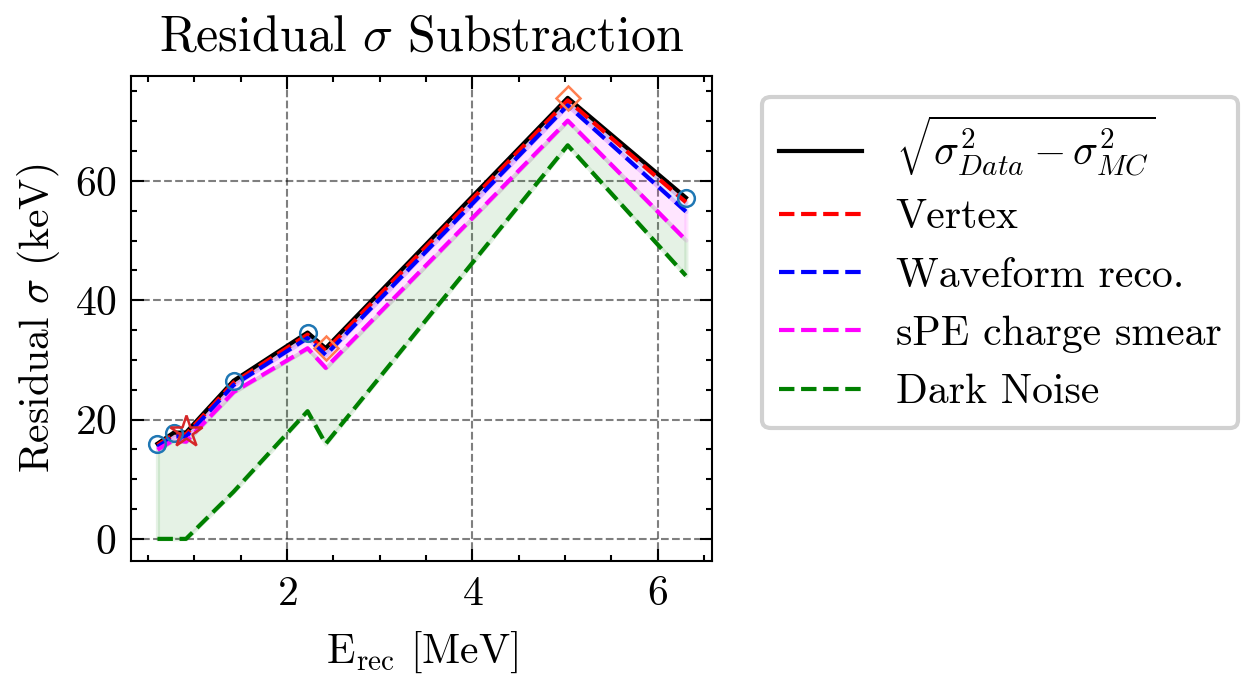
\includegraphics[width=0.7\textwidth]{4_efficiency/residual_sigma_subtraction.png}
    \caption{Decomposition of the residual energy resolution $\sigma_{\text{res}}$. The black solid line is the total $\sigma_{\text{res}} = \sqrt{\sigma_{\text{Data}}^2 - \sigma_{\text{MC}}^2}$. The colored dashed lines show the residual after sequentially subtracting, in quadrature, the contributions from: Dark Noise (estimated based on real data), sPE charge smearing (purple), waveform reconstruction (blue), and vertex reconstruction (red).}
    \label{fig:residual_decomposition}
\end{figure}

\paragraph{Future Work: Full-Chain Simulation and Quantification}
The origin of the energy-proportional residual contribution requires further investigation. We are currently developing a complete \textbf{full-chain simulation} workflow, encompassing the data-driven SPE model, to the application of the full reconstruction algorithms (including vertex and waveform reconstruction). This will help us quantify the intrinsic performance limits introduced by the SPE, waveform reconstruction, and energy-vertex reconstruction algorithms of OMILRec. 

\subsection{Reactor related uncertainty}
The accurate prediction of the reactor antineutrino flux and spectrum depends on several reactor-related parameters, each contributing to the total systematic uncertainty. These include the precise measurement of the reactor's thermal power, the understanding of the energy released per fission, the evolving fission fractions of the four primary isotopes throughout the fuel cycle, and corrections for effects like the non-equilibrium of long-lived fission fragments and the antineutrino emission from spent nuclear fuel. Comprehensive simulations of the reactor core, validated against operational data, are used to track the complex evolution of the fuel composition. The uncertainties from these reactor physics aspects are major contributors to the overall uncertainty in the predicted antineutrino signal at the JUNO experiment.

These uncertainties are kind of complicated and it is hard to define whether they are fully reactor-correlated or reactor-uncorrelated. 
Therefore, some tests are done by defining their reactor correlation and they are used to check which treatment is more conservative. 

\subsubsection{Reactor power}
Based on the experience from Daya Bay experiment, the thermal power of the reactor cores is mainly monitored by three systems. Accounting for correlations and calibration differences, the uncertainty of the KIT/KDO system, which provides hourly thermal power data to the experiment, is estimated to be 0.5\%. 
In this study, the reactor power uncertainties are handled core-by-core, assuming full correlation among cores within the same NPP and no correlation across different NPPs.

Some configurations are set and tests are done. 
\begin{itemize}
        \item Config. 1: Core-by-core uncorrelated 
        \[
        \chi^2_{\text{RUC}} = \sum_{r} \left( \frac{\alpha_r}{\sigma_r} \right)^2
        \]
        \item Config. 2: Core-by-core in same NPP correlated, but NPP-by-NPP uncorrelated 
        \[
        \chi^2_{\text{RUC}} = \sum_{p} \left( \frac{\alpha_p}{\sigma_p} \right)^2 
        \]
    \end{itemize}
    
    \vspace{0.5em}
    \begin{tabular}{|l|c|c|c|}
        \hline
        \textbf{50 days} & $\Delta m^2_{31}$ precision [\%] & $\sin^2\theta_{12}$ precision [\%] & $\Delta m^2_{21}$ precision [\%] \\
        \hline
        Config. 1 & 1.141 & 2.383 & 1.311 \\
        \hline
        Config. 2 & 1.141 & 2.386 & 1.311 \\
        \hline
    \end{tabular}
   
    It is found that the config. 2 produces a more conservative results. 


\subsubsection{Fission energy}
The energy released per fission for each isotope is defined as the energy converted to heat over a finite time, accounting for energy carried by neutrinos and captures on non-fissile materials. 
As studied by Daya Bay experiment, the fission energy is not a fixed fundamental constant but depends on the reactor environment.
In this study, the uncertainties of fission energy are handled assuming full correlation among cores.


\subsubsection{Fission fraction}
Electron antineutrinos are produced from the beta decays of fragments from four primary fission isotopes: $^{235}\rm U$, $^{238}\rm U$, $^{239}\rm{Pu}$, $^{241}\rm{Pu}$. Their relative contributions, or fission fractions change dynamically with fuel burn-up. 
The Daya Bay nuclear power plant provides detailed simulations of this evolution using the validated SCIENCE/APOLLO2 software package. Comparisons between APOLLO2 calculations and direct measurements of spent fuel isotopic content show deviations of less than 5\%. 
Therefore, the uncertainty for each fission fraction is conservatively estimated to be 5\%. These fractions are strongly correlated, as the consumption of uraiunm and production of plutonium isotopes are linked. A correlation matrix is used for proper uncertainty propagation.
JUNO alaysis follows the similar strategy as the Daya Bay analysis. 
In this study, the uncertainties of fission fractions are handled assuming full correlation among cores.


\subsubsection{Spent fuel}
Long-lived fission isotopes within the spent nuclear fuel(SNF) continue to beta-decay, producing an additional source of antineutrinos. The contribution from SNF is calculated by identifying isotopes with half-lives longer than 10 hours and whose decays exceed the inverse beta decay threshold. Using the refueling history and SNF inventory provided by the plant, the cumulative yield and spectrum of these isotopes are computed. 
In this study, the rate uncertainties of SNF spectrum are handled core-by-core, assuming full correlation among cores within the same NPP and no correlation across different NPPs. The shape uncertainties are neglected.


\subsubsection{Non-equilibrium}
The long-lived fission fragments need some time to reach equilibrium between their production and decay rates. 
In an operating reactor core, these fragments accumulate, and their decays contribute extra antineutrinos, known as the non-equilibrium (NonEq) contribution.
In this study, the rate uncertainties of NonEq spectrum are handled core-by-core, assuming full correlation among cores within the same NPP and no correlation across different NPPs. The shape uncertainties are neglected.

\subsubsection{Reference spectrum}
Systematic uncertainties in the IBD yield is dominated by the reference spectrum used in this analysis, which is measured with an uncertainty of 1.2\% from the DayaBay paper~\cite{DYB:Flux2025}.
The IBD yield,  $5.84 \pm 0.07 \times 10^{-43}$~cm$^2$/fission, includes the uncertainties from the IBD cross section, the thermal power, fission fractions and fission energy from Daya Bay and Lingao reactor power plant.
The uncertainty of the IBD cross section is fully correlation between Daya Bay and JUNO, and thus shall not consider the cross section uncertainty in JUNO.
Weighted by the thermal power and baseline of each reactor core or nuclear power plant, the average fission fractions in the JUNO data were 0.564, 0.076, 0.303, and 0.058 for $^{235}$U, $^{238}$U, $^{239}$Pu, and $^{241}$Pu, respectively. In comparison, the corresponding values in the Daya Bay data were 0.564, 0.076, 0.304 and 0.056~\cite{DYB:Flux2025}.
Consequently, they shared a $>$\,99\% common reactor antineutrino spectrum, which we denote as the model-independent component shared by both the JUNO and Daya Bay datasets.
The differences in the fission fractions between JUNO and Daya Bay resulted in a $<$0.1\% uncertainty in the flux, assuming a 10\% uncertainty in the isotopic reference spectra.


\subsubsection{Summary}

\begin{table}[!htbp]
    \caption{Summary of the systematic uncertainties of the predicted integrated reactor antineutrino flux associated with a single reactor core.}
    \label{tab:reactorErr}
    \centering
    \footnotesize% fontsize
    \setlength{\tabcolsep}{4pt}% column separation
    \renewcommand{\arraystretch}{1.2}%row space 
    \begin{tabular}{lc}
        \hline
        Parameter & Uncertainty \\ 
        \hline
        power & 0.5\% \\
        energy/fission & 0.2\% \\
        reference spectrum & 1.2\% \\
        different fission fraction & 0.1\% \\
        fission fraction & 0.6\% \\
        spent nuclear fuel & 0.3\% \\
        non-equilibrium & 0.2\% \\
        \hline 
    \end{tabular}
\end{table}


% \section{Validations for the unbiasing policy}
% Reference: 

% Technote: DocDB-14803.

% Requirement: DocDB-14804.
\section{Oscillation analysis}
\begin{figure}[h]
    \centering
    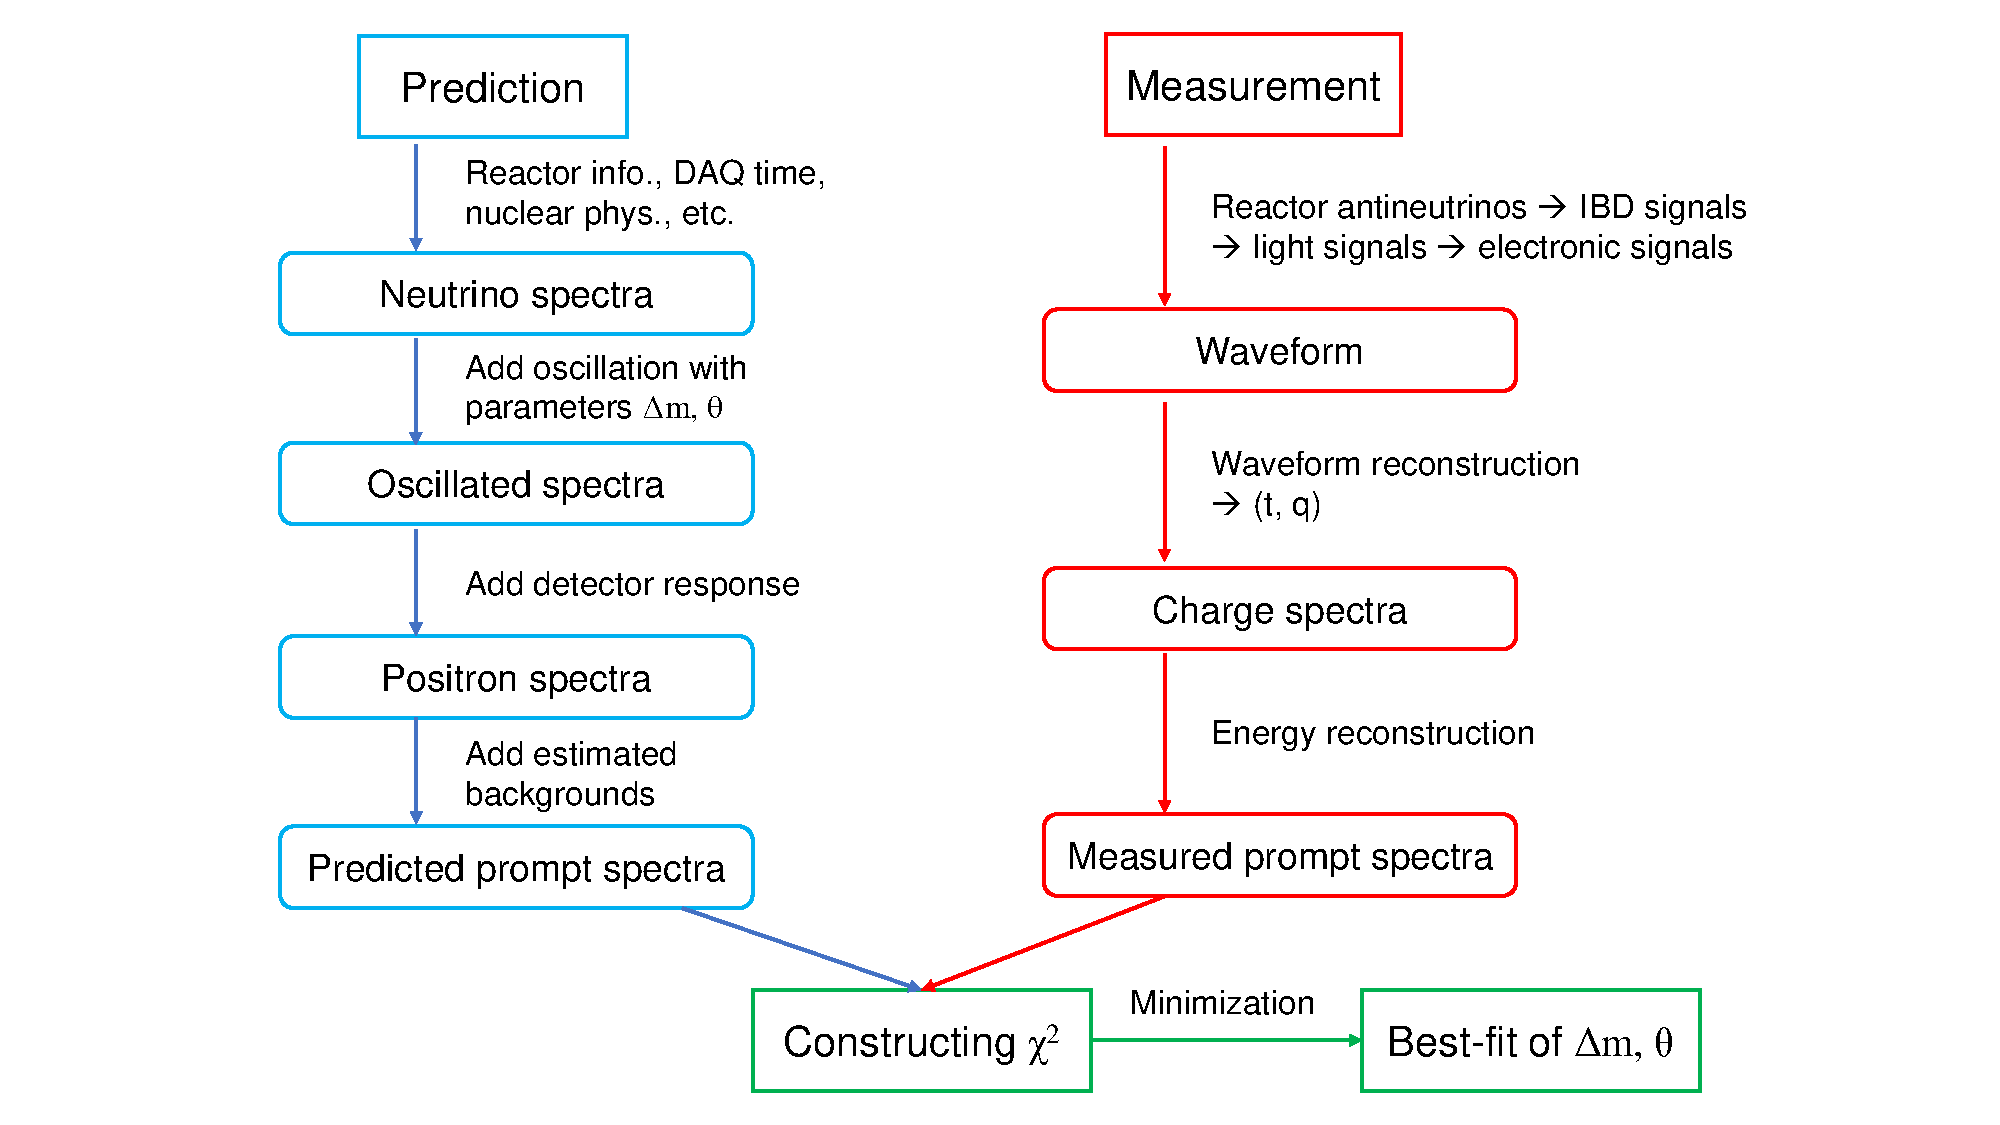
\includegraphics[width=16cm]{5_oscillation/oscAnaDiagram.pdf}
    \caption{Schematic diagram of the oscillation analysis.}
    \label{fig:oscAnaDiagram}
\end{figure}



\subsection{Statistical Analysis Framework}

This subsection defines the core statistical framework for extracting oscillation parameters
($\sin^2\theta_{12}$, $\Delta m^2_{21}$, $\Delta m^2_{31}$) from JUNO data.

\subsubsection{The statistical method}

We predict the binned reconstructed-energy spectrum $\boldsymbol{T}(\theta,\alpha)$ from
oscillation parameters $\theta$ and nuisance parameters $\alpha$ (detector, backgrounds, reactor),
where $\theta=(\sin^2\theta_{12},\Delta m^2_{21},\Delta m^2_{31},\sin^2\theta_{13})$.

With observed JUNO spectrum $\boldsymbol{M}$, We employ the least-squares method and construct a binned $\chi^2$ with pull terms to account for the impact of systematic uncertainties 
% \begin{equation}
%   \chi^2_{\mathrm{CNP}}(\theta,\nu) = \sum_i \frac{(n_i-\mu_i)^2}{\sigma_i^2}, \quad
%   \sigma_i^2 = \tfrac{1}{3}\,n_i + \tfrac{2}{3}\,\mu_i \label{eq:cnp}
% \end{equation}
\begin{equation}
    \begin{split}
        \chi^2_{\rm JUNO} \equiv &\sum_i^{Nbins}{\left(\frac{\left(M_i-T_i^{\rm IBD}\left(\alpha_C,\alpha_D,\alpha_l,\alpha_\eta,\dotsb\right)-\sum_B^{\rm Bkg}{\left(T_i^{B}(\alpha_B)\right)}\right)^2}{V_{ii}^{\rm stat}+\sum_B^{\rm Bkg}{\left(T_i^{B}(\alpha_B)\cdot \sigma_{\rm shp}^B\right)^2}})\right)}\\
        &+\left(\frac{\alpha_C}{\sigma_C}\right)^2+\sum_p^{\rm Plants}{\left(\frac{\alpha_{\rm Pow}^p}{\sigma_{\rm Pow}^p}\right)^2}+\sum_p^{\rm Plants}{\left(\frac{\alpha_{\rm SNF}^p}{\sigma_{\rm SNF}^p}\right)^2}+\sum_p^{\rm Plants}{\left(\frac{\alpha_{\rm NonEq}^p}{\sigma_{\rm NonEq}^p}\right)^2}+\frac{\boldsymbol{\alpha}_{\mathrm{FF}}^{\!\top}\,\boldsymbol{\rho}_{\mathrm{FF}}^{-1}\,\boldsymbol{\alpha}_{\mathrm{FF}}}{\sigma_{\mathrm{FF}}^{2}}\\
        &+\left(\frac{\alpha_D}{\sigma_D}\right)^2+\sum_{l=1}^{4}{\left(\frac{\alpha_l}{\sigma_l}\right)^2}+\left(\frac{\alpha_{\rm EScale}}{\sigma_{\rm EScale}}\right)^2+\sum_{\eta=a,b,c}\left(\frac{\alpha_{\eta}}{\sigma_{\eta}}\right)^2+\sum_{f=1}^{4}\left(\frac{\alpha_{\rm FE}^{f}}{\sigma_{\rm FE}^{f}}\right)^2\\
        &+\sum_B^{\rm Bkg}{\left(\frac{\alpha_B}{\sigma_B}\right)^2}+\left(\frac{\alpha_{\rm Th/U}}{\sigma_{\rm Th/U}}\right)^2+\sum_{k=1}^{5}{\left(\frac{\alpha^k_{\rm AtmShp}}{\sigma^k_{\rm AtmShp}}\right)^2}+\left(\frac{\alpha_{\rho ME}}{\sigma_{\rho ME}}\right)^2,
    \end{split}
    \label{eq:chisq:JUNO}
\end{equation}
where $M_i$ is measured total event number in i-the energy bin, which is the summation of signal and background. And $T_i^{\rm IBD}$ is the predicted IBD signal event number, which depends on the oscillation parameters of interest and will be described in Sec.~\ref{subsubsec:obs-spectrum}. $T_i^{B}$ is the estimated background event number of B-th kind of background, and the estimation procedure is listed in Sec.~\ref{sec:background}. The meaning of the indices in the chi-square formula are listed below:
\begin{itemize}
    \item i, refers to i-th energy bin;
    \item C, refers to reactor-related correlated uncertainty;
    \item D, refers to the detection efficiency uncertainty;
    \item B, refers to B-th background;
    \item l, refers to l-th liquid scintillator nonlinearity pull curve;
    \item EScale, refers to the absolute energy scale;
    \item $\eta$ (a,b,c) refers to energy resolution parameters;
    \item p, refers to p-th nuclear power plant;
    \item Pow, refers to thermal power;
    \item shp, refers to the spectrum shape uncertainties;
    \item $\rho_{ME}$, refers the matter density;
    \item NonEq, refers to the non-equilibrium;
    \item SNF, refers to the spent nuclear fuel;
    \item $\rm Th/U$, refers to the ratio of isotope Th to U for geo-neutrino;
    \item AtmShp, refers to the atmospheric-$\nu$ shape uncertainty;
    \item f, refers to 4 isotopes $^{235}U$, $^{238}U$, $^{239}Pu$, $^{241}Pu$;
    \item FF, refers to fission fractions for 4 isotopes;
    \item FE, refers to fission energy for 4 isotopes.
\end{itemize}
The $V_{ii}^{\rm stat}$ denotes statistical variance combines Neyman ($\sigma^2 \approx M$) and Pearson ($\sigma^2 \approx T$) statistics
\begin{equation}
    V_{ii}^{\rm stat}  \equiv 3\cdot\left(\frac{1}{M_i}+\frac{2}{T_i^{\rm IBD}+\sum_B^{\rm Bkg}T_i^{B}}\right)^{-1}\label{eq:Chisq:CNP},
\end{equation}
which exhibit biases in opposite directions. Their weighted combination eliminates first-order bias relative to the Poisson likelihood, improving parameter estimates while avoiding zero-bin failures.

The Daya Bay spectrum data are analyzed using a $\chi^2$ statistic constructed with the full covariance matrix:
% \begin{equation}
%   \chi^2_{\text{Pearson, DYB}} = \sum_k \frac{(n_k^{\text{DYB}}-\mu_k^{\text{DYB}})^2}{n_k^{\text{DYB}}} \label{eq:pearson}
% \end{equation}
\begin{equation}
    \chi^2_{\text{DYB}} = (\boldsymbol{M}^{\rm DYB} - \boldsymbol{T}^{\rm DYB})^T\mathbf{Cov}^{-1}(\boldsymbol{M}^{\rm DYB} - \boldsymbol{T}^{\rm DYB})\label{eq:Chisq:DYB},
\end{equation}
where $\boldsymbol{M}^{\rm DYB}$ is measured prompt energy spectrum from Ref.~\cite{DYB:Flux2025}, normalized to the spectrum per fission, after removing the effects of oscillation, spent nuclear fuel correction, and non-equilibrium correction. And $\boldsymbol{T}^{\rm DYB}$ is the predicted spectrum obtained using the detector response matrix from Ref.~\cite{DYB:Flux2025}, incorporating IBD cross section, liquid scintillator non-linearity, energy resolution, and inner acrylic vessel effect (IAV). Ref.~\cite{DYB:Flux2025} also provided the full covariance matrix $\mathbf{Cov}$ including statistical uncertainty and systematic uncertainties from detection, backgrounds, and reactors.

% External constraints enter as Gaussian pulls, with nuisance parameters $\alpha_j$ re-centered at zero:
% \begin{equation}
%   \chi^2_{\text{pull}} = \sum_j \left(\frac{\alpha_j}{\sigma_j}\right)^2 \label{eq:pull}
% \end{equation}

In addition to the pull terms for systematic uncertainties, external constraints on $\rm{sin}^2\theta_{13}$ and $\Delta m^2_{31}$ from the Daya Bay measurement~\cite{an2023precision} are also included in Sec.\ref{subsec:analysis:result}. The \textbf{total objective} to be minimized is therefore

\begin{equation}
\chi^2_{\text{Total}}
= \chi^2_{\text{JUNO}} + \chi^2_{\text{DYB}}
+ \left( \frac{\sin^2\theta_{13} - \sin^2\theta_{13}^{\rm DYB}}{\sigma(\sin^2\theta_{13}^{\rm DYB})} \right)^2
+ \left( \frac{\Delta m_{31}^2 - \Delta m_{31}^{2,\,\rm DYB}}{\sigma(\Delta m_{31}^{2,\,\rm DYB})} \right)^2 ,
\label{eq:Chisq:Total}
\end{equation}

\subsubsection{The observed spectrum prediction}
\label{subsubsec:obs-spectrum}
With the prompt energy distribution, we calculate the expected event number $T_{i}^{IBD}$ for i-th energy bin with Eq.~\eqref{eq:DetectorResponse:further}, which is needed for calculating the chi-square defined in Eq.~\eqref{eq:chisq:JUNO}.

\begin{equation}
    T_i^{IBD} \equiv (1+\alpha_C+\alpha_D)\cdot\int_{E^i_{\rm{rec}}}^{E^{i+1}_{\rm{rec}}}dE_{\rm{rec}}\int_{1.8}^{13} dE_{\bar{\nu}_e}\cdot S_0(E_{\bar{\nu}})\cdot R(E_{\bar{\nu}_e}, E_{\rm{rec}}),
    \label{eq:DetectorResponse:further}
\end{equation}
where $E_i$ and $E_{i+1}$ are the lower and upper edges of i-th energy bin, respectively. Both $\alpha_C$ and $\alpha_D$ are the nuisance parameters that float the overall normalization of the spectrum, corresponding to reactor-related correlated uncertainty and detection efficiency uncertainty, respectively. In the following, we sequentially describe the components of the expected antineutrino energy spectrum $S_0(E_{\bar{\nu}})$ arriving at JUNO, as well as the detector response function $R(E_{\bar{\nu}_e}, E_{\rm{rec}})$. 

The IBD signal detected at JUNO originates from ten reactor cores, whose effective thermal power, baselines, and effective fission fractions are summarized in Table~\ref{tab:ReactorInfo}. The effective thermal power and effective fission fractions are obtained by averaging the weekly reactor power and isotope-dependent fission numbers over the data-taking period. The IBD rate without selection efficiency for each core is also listed based on oscillation parameters from PDG 2024.

\begin{table}[ht]
    \centering
    \begin{tabular}{c|c|c|c|c|c|c|c}\hline
        Core    &   Power (GW)   &   Baseline (km)   &   $ff_{235U}$ &   $ff_{238U}$ & $ff_{239Pu}$ & $ff_{241Pu}$ & IBD rate ($\rm day^{-1}$)    \\ \hline
        TS-C1    & 4.09 & 52.77 & 0.670 & 0.076 & 0.223 & 0.031 & 8.53\\ 
        TS-C2    & 4.15 & 52.64 & 0.464 & 0.078 & 0.373 & 0.085 & 8.06\\ 
        YJ-C1    & 1.91 & 52.74 & 0.553 & 0.075 & 0.304 & 0.068 & 3.81\\ 
        YJ-C2    & 2.74 & 52.82 & 0.592 & 0.075 & 0.288 & 0.045 & 5.53\\ 
        YJ-C3    & 2.86 & 52.41 & 0.497 & 0.076 & 0.354 & 0.073 & 5.70\\ 
        YJ-C4    & 1.55 & 52.49 & 0.720 & 0.073 & 0.175 & 0.032 & 3.35\\ 
        YJ-C5    & 2.47 & 52.11 & 0.583 & 0.075 & 0.295 & 0.047 & 5.16\\ 
        YJ-C6    & 2.87 & 52.19 & 0.510 & 0.076 & 0.345 & 0.069 & 5.79\\ 
        DYB      & 15.90 & 215  & 0.549 & 0.076 & 0.315 & 0.060 & 3.37\\ 
        FCG      & 9.28 & 411   & 0.580 & 0.070 & 0.300 & 0.050 & 0.55\\ \hline
        All      & —     & —     & —     & —     & —     & —     & 49.84\\ \hline
    \end{tabular}
    \caption{Summary of unblind effective thermal power, baseline, effective fission fraction distribution of Yangjiang (YJ) and Taishan (TS) reactor complexes, as well as remote Daya Bay (DYB) reactor and Fangchenggang (FCG) reactor. }
    \label{tab:ReactorInfo}%
\end{table}%
The neutrino energy spectrum, $S_0(E_{\bar{\nu}_e})$ at JUNO in data-taking period, given by Eq.~\eqref{equ_generic}, is calculated with reactor antineutrino flux $\phi_r(E_{\nu})$ multiplied by electron antineutrino survival probability in Eq.~\eqref{eq:P_nue2nue}, with corresponding thermal power and baseline of the reactors.
\begin{equation}\label{equ_generic}
    S_0(E_{\nu},T_{\rm live})  = T_{\rm live} \cdot \sum_r \frac{P_{ee}(E_{\nu},L_{r})}{ 4\pi L^2_{r}}\phi_r(E_{\nu}),
\end{equation}
where $E_{\nu}$ is the $\bar\nu_e$ energy, $r$ is the reactor index, $L_{r}$ is the distance from detector to reactor $r$, $T_{\rm live}$ is the total DAQ live time, and $P_{ee}(E_{\nu},L_{r})$ is the $\bar{\nu}_e$ survival probability expressed as
\begin{equation}\label{eq:P_nue2nue}
    \begin{aligned}
        P_{\bar{\nu}_e\to\bar{\nu}_e}=1 & -\sin^22\theta_{13}(\cos^2\theta_{12}\sin^2\Delta_{31}+\sin^2\theta_{12}\sin^2\Delta_{32}) \\
                                        & -\cos^4\theta_{13}\sin^22\theta_{12}\sin^2\Delta_{21},
    \end{aligned}
\end{equation}
where $\Delta_{ji}=\Delta m_{ji}^2L/(4E)=(m_j^2-m_i^2)L/(4E)$, in which L is the baseline and E is antineutrino energy. The correction from matter effect~\cite{Khan:2019doq} on the survival probability is also included. The $\phi_r(E_{\nu})$ in Eq.\eqref{equ_generic} is the average antineutrino energy spectrum emitted per second from reactor $r$. 
\begin{equation}\label{equ_prediction}
    \phi_r(E_{\nu}) = \frac{W_r}{\sum_i f_{ir} \cdot e_i}\sum_i f_{ir} \cdot S_i(E_{\nu}),
\end{equation}
where $W_r(t)$ is the thermal power of reactor $r$, $e_i$ is the mean energy released per fission for isotope $i$, $f_{ir}(t)$ is the fission fraction. $S_i(E_{\nu})$ is the $\bar\nu_e$ energy spectrum per fission for i-th isotope, which is calculated by exponential interpolating the listed values from Huber in Ref.~\cite{Huber:2011wv} ($^{235}$U, $^{239}$Pu, and $^{241}$Pu) and Mueller in Ref.~\cite{Mueller:2011nm} ($^{238}$U). The values of fission fraction and fission energy used are listed in Table~\ref{tab:ReactorInfo}.
In the combined analysis using the JUNO and DYB near-detector measured spectra, the calculation of $\phi_r(E_{\nu})$ is modified accordingly. The detailed procedure for this modification, including the method for combining JUNO and DYB data, is described in Sec.~\ref{subsec:FluxInComb}.

The beta decay rate of some long-lived fission fragments will not reach equilibrium with their production rate. The non-equilibrium fission fragments will then accumulate in the reactor core, and their beta decay will contribute $\sim$0.6\% additional antineutrinos\cite{Mueller:2011nm}.

The burned nuclear fuel removed to a cooling pool near the reactor core is stored as spent nuclear fuel (SNF), the long-lived isotopes in which will also contribute $\sim$0.2\% additional antineutrinos in our analysis. Thus, the antineutrino energy spectrum $\phi_r(E_{\nu})$ is modified to cover the contributions of SNF and non-equilibrium (NonEq) effect as shown in Eq.~\eqref{eq:phi:SNF-NonEq}.
\begin{equation}
    \phi^\prime_r(E_{\nu})=\phi_r(E_{\nu})+\phi_r^{\rm HM}(E_{\nu}) \cdot f_{\rm NonEq}^r(E_{\nu})\cdot \left(1+\alpha_{\rm NonEq}^r\right)+\phi_{\rm SNF}^{r,\rm Abs}(E_{\nu})\cdot\left(1+\alpha_{\rm SNF}^r\right),
    \label{eq:phi:SNF-NonEq}
\end{equation}
where $f_{\rm NonEq}^r$ is the relative contribution of the NonEq effect to the antineutrion energy spectrum $\phi_r^{\rm HM}(E_{\nu})$ predicted by the Huber-Mueller model for reactor $r$, evaluated using the corresponding fuel history. The term $\phi_{\rm SNF}^{r,\rm Abs}(E_{\nu})$ gives the absolute SNF contribution per second derived from core simulation for reactor $r$. In particular, reactors YJ-C1 and YJ-C4 include an additional shutdown SNF component due to their recent shutdown operations.

For the part of detector response, we assume the energy leakage is negligibly small. Therefore, the deposited energy of positron $E_{\rm dep}$ in the liquid scintillator can be expressed in Eq.~\eqref{eq:E_dep}.

\begin{equation}
    % E_{\rm dep}=E_{e^+}+0.511\ {\rm{MeV}}.
    E_{\rm dep}=T_{e^+}+2\times0.511\ {\rm{MeV}},
    \label{eq:E_dep}
\end{equation}
where $T_{e^+}$ is the kinetic energy of positron. The positron energy $E_{e^+}=T_{e^+}+0.511~\rm{MeV}$ is function of the scattering angle $\cos\theta$ and antineutrino energy $E_{\bar{\nu}}$ in the IBD interaction. There are two widely used formulae of IBD cross-section. One is evaluated by Vogel and Beacom~\cite{Vogel:1999zy}, the other is calculated by Strumia and Vissani~\cite{Strumia:2003zx}. In this analysis, we adopt the Vogel–Beacom cross section for the prediction. Besides expressing the cross section in terms of the scattering angle, $\frac{d\sigma}{d\cos\theta}(E_{\bar{\nu}},\cos\theta)$, it can also be formulated as a function of the deposited energy through a variable substitution, $\frac{d\sigma}{dE_{e^+}}(E_{\bar{\nu}},E_{e^+})$~\cite{Vogel:1999zy}.
So the exact formula of the detector response function $R(E_{\bar{\nu}_e}, E_{\rm{rec}})$ in Eq.~\eqref{eq:DetectorResponse:further} can be expressed as Eq.~\eqref{eq:DetectorResponse:Full} shows.
\begin{equation}
    R(E_{\bar{\nu}_e}, E_{\rm{rec}}) \equiv \int_{0.8}^{12} dE_{\rm dep} \cdot \frac{d\sigma}{dE_{e^+}}(E_{\bar{\nu}},E_{e^+})
    \cdot N_p \cdot \epsilon \cdot
    \frac{1}{\sigma_{E_{\rm vis}}\sqrt{2\pi}}\cdot
    \exp{\left(-\frac{1}{2}\left(\frac{E_{\rm{rec}}-E_{\rm vis}\left(E_{\rm dep}\right)}{\sigma_{E_{\rm vis}}}\right)^2\right)},
    \label{eq:DetectorResponse:Full}
\end{equation}
where the prompt energy $E_{\rm{rec}}$ refers to the observed (smeared) visible energy of prompt signal, $N_p$ is the number of target proton number $(1.442\pm0.014)\times10^{33}$, and $\epsilon$ is the total IBD selection efficiency listed in Tabel~\ref{tab:DetErr}. The expected visible energy $E_{\rm vis}$ here is evaluated with LS nonlinearity in Eq.~\eqref{eq:LSNL:definition} and deposited positron energy.
\begin{equation}
    E_{\rm vis}\left(E_{\rm dep}\right)=f_{\rm LSNL}(E_{\rm dep})\cdot E_{\rm dep},
    \label{eq:LSNL:definition}
\end{equation}
\begin{equation}
    f_{\rm LSNL}(E_{\rm dep}) = \left( 1+\alpha_{\rm EScale} \right) \cdot \left( f_{\rm LSNL}^{\rm norm}(E_{\rm dep})+\sum_{l=1}^{4}\left(f_{\rm LSNL}^{l}(E_{\rm dep})-f_{\rm LSNL}^{\rm norm}(E_{\rm dep})\right) \cdot \alpha_{l} \right),
    \label{eq:LSNL:correction}
\end{equation}
where $f_{\rm LSNL}^{\rm norm}(E_{\rm dep})$ is the nominal LSNL curve, and $f_{\rm LSNL}^{l}(E_{\rm dep})$ is $l$-th pull curve to float the final LSNL curve.

The generic parameterization formula in Eq.~\eqref{eq:EnergyResolution:abc} shows the fractional energy resolution for visible energy in MeV.

\begin{equation}
    \frac{\sigma_{E_{\rm vis}}}{E_{\rm vis}}=\sqrt{\left(\frac{a}{\sqrt{E_{\rm vis}}}\right)^2+b^2+\left(\frac{c}{E_{\rm vis}}\right)^2}.
    \label{eq:EnergyResolution:abc}
\end{equation}
The detail of energy resolution has been discussed in Sec.~\ref{subsubsection:EReso}.

\subsubsection{Estimation and Inference}

\paragraph{Lane 1: Estimation (Best Fit)}
Find parameters that minimize Eq.~\eqref{eq:Chisq:Total}:
\begin{equation}
  (\hat\theta,\hat\nu) = \arg\min_{\theta,\nu} \chi^2_{\text{tot}} \label{eq:bestfit}
\end{equation}

\paragraph{Lane 2: Inference (Confidence Regions)}
Profile-likelihood ratio for parameter $\theta$:
\begin{equation}
  \Delta\chi^2(\theta) = \chi^2_{\text{tot}}(\theta,\hat\nu_\theta) - \chi^2_{\min} \label{eq:profile}
\end{equation}
where $\hat\nu_\theta$ minimizes $\chi^2_{\text{tot}}$ for fixed $\theta$ (profiling).

\textbf{Critical point:} With 50-day statistics and many nuisances, Wilks' theorem
does not apply. Critical $\Delta\chi^2$ values are \textbf{empirically determined}
via toy MC.

\paragraph{Confidence Intervals}
Report 1D and 2D intervals using \textbf{toy-calibrated} critical $\Delta\chi^2$;
state actual quantiles used (e.g., 68\% $\rightarrow \Delta\chi^2_{\text{crit}} = 1.05$).
Distinguish Asimov sensitivity (expectation) from data significance (after unblinding).

\subsubsection{Systematics Treatment}

\paragraph{Nuisance-Parameter Policy}
\textbf{Baseline:} Profile nuisances with Gaussian pulls; monitor pull sizes and physicality.
\textbf{Switch criteria:} Marginalize if coverage fails, pulls become unphysical, or overfitting markers appear.

\paragraph{Toy-MC Engine}
Algorithm (1D example):
\begin{enumerate}
  \item \textbf{Parallel universes:} Sample external centers $\alpha^0 \sim \mathcal{N}(0, \sigma)$
  \item \textbf{Generate toy data:} $n_i \sim \text{Poisson}(\mu_i(\theta^{\text{true}}, \alpha^{\text{true}}))$ for 50-day exposure
  \item \textbf{Fit each toy:} Minimize Eq.~\eqref{eq:Chisq:Total} $\rightarrow$ get $\chi^2_{\min}$ and $\Delta\chi^2(\theta)$ profile
  \item \textbf{Aggregate:} Collect $\Delta\chi^2$ across toys; take 68\%/95\% quantiles as critical values
  \item \textbf{Coverage test:} Verify that 68\% of toys have truth in 1$\sigma$ interval
\end{enumerate}

For 2D parameter pairs, use empirical critical values (e.g., 68\% $\rightarrow \Delta\chi^2_{\text{crit}} \approx 2.3$ in Wilks limit, verify with toys).

\paragraph{Implementation Note}
We sample $\alpha^{\text{truth}} \sim \mathcal{N}(0, \sigma)$, generate toy data with $(\theta^{\text{true}}, \alpha^{\text{truth}})$,
then fit with $\chi^2_{\text{pull}} = \sum_j (\alpha_j/\sigma_j)^2$ (i.e., $\alpha^0=0$).
This creates inconsistency between generation truth and fit centers, properly accounting for systematic uncertainties.


\subsection{Semi-Model-Independent Approach}
\label{subsec:FluxInComb}

The reactor spectrum is the dominant systematic. We employ a semi-model-independent
approach: DYB data constrains the baseline spectrum shape; theoretical HM predictions
enter only for JUNO-specific corrections (different cores, SNF, equilibrium adjustments).

\subsubsection{DYB-Anchored Reactor Spectrum}

Represent DYB spectrum as:
\begin{equation}
  S_{\text{DYB}}(E) = S_0(E) + \sum_{i=1}^{N} \alpha_i B_i(E)
\end{equation}

\begin{itemize}
  \item $S_0(E)$: Nominal Huber-Mueller (HM) prediction based on short-irradiation ILL data
  \item $B_i(E)$: Segment basis function ($= S_0(E)$ in segment $i$, zero elsewhere)
  \item $\alpha_i$: Coefficients constrained by DYB data
  \item $N$: Number of segments (tunable parameter, optimized to $N^* = 15$)
\end{itemize}

JUNO spectrum includes corrections:
\begin{equation}
  S_{\text{JUNO}}(E) = S_{\text{DYB}}(E) + \Delta S(E)
\end{equation}
where $\Delta S$ accounts for: (1) fission fraction differences between JUNO and DYB cores,
(2) spent nuclear fuel (SNF), and (3--7) five off-equilibrium corrections to the HM model. The antineutrino energy spectrum in Eq.~\eqref{equ_prediction} depends on the Huber-Mueller flux model. \textbf{In the semi-model-independent approach, it is replaced by Eq.~\eqref{equ_prediction_in_comb}}
\begin{equation}\label{equ_prediction_in_comb}
    \phi_r(E_{\nu}) = \frac{W_r}{\sum_i f_{ir} \cdot e_i} \cdot \left(S_{\rm DYB}(E_\nu)+\sum_i\left(f_{ir}^{\rm JUNO}-f_i^{\rm DYB}\right) \cdot S_{i}^{\rm model}(E_\nu)\right),
\end{equation}
where $f_{r}^{\rm JUNO}$ is the average fission fractions of the four isotopes for reactor $r$ on the JUNO side, while $f^{\rm DYB}$ is average fission fraction in the DYB measurement of reactor flux, $\rm ^{235}U : ^{238}U : ^{239}Pu : ^{241}Pu = 0.564:0.076:0.304:0.056$. The second term in the outer bracket of Eq.~\eqref{equ_prediction_in_comb} accounts for the spectral distortion introduced by the differing fission fractions of reactor $r$ relative to the DYB reference. The implementation of this correction is model-dependent and is described in the following subsubsection.

\subsubsection{Model-Dependent Corrections}

The difference $\Delta S$ uses Huber-Mueller (HM) theoretical predictions for JUNO and DYB separately,
then takes the difference to minimize reliance on absolute theoretical uncertainties (reactor anomaly).

\paragraph{JUNO Configuration}
JUNO reactors operate in equilibrium at $\sim$53~km. SNF contributions are measurable;
off-equilibrium corrections adjust HM to match equilibrium conditions.

For JUNO core $i$:
{\small
\begin{align}
  S_{\text{J},\, i}^{\text{HM}}(E) &= (1{+}\asnf{J,i}) \cdot S^{\text{SNF}}(E) \notag \\
   &\quad + \sum_{j,k} F_{\text{J},i,j} \cdot \left(S^{\text{HM}}_j(E) {+}\ahm{k} \cdot\delta S^{\text{HM}}_{j,k}(E) {+}(1{+}\aneq{J,i,j}) \cdot S_j^{\text{NEQ}}(E)\right)
\end{align}
}

\paragraph{DYB Configuration}
DYB reactors operate in equilibrium at $\sim$500~m; SNF is negligible and removed.

For DYB:
{\small
\begin{equation}
  S_{\text{D}}^{\text{HM}}(E) = \sum_{j,k} F_{\text{D},j} \cdot \left(S^{\text{HM}}_j(E) {+} \ahm{k} \cdot\delta S^{\text{HM}}_{j,k}(E) {+} (1{+}\aneq{D}) \cdot S_j^{\text{NEQ}}(E)\right)
\end{equation}
}

\paragraph{Difference Expansion}
The difference $\Delta S_i(E) = S_{\text{J},i}^{\text{HM}}(E) - S_{\text{D}}^{\text{HM}}(E)$ expands to:
{\small
\begin{align}
  \Delta S_i(E) & = \sum_{j} \Delta F_{i,j} \cdot S^{\text{HM}}_j(E) + (1{+}\asnf{J,i}) \cdot S^{\text{SNF}}(E) \notag \\
   & \quad + \sum_{j,k} \Delta F_{i,j} \cdot \ahm{k} \cdot \delta S^{\text{HM}}_{j,k}(E) \notag \\
   & \quad + \sum_{j} F_{\text{J},i,j} \cdot \Delta \alpha_{\text{NEQ},i,j} \cdot S_j^{\text{NEQ}}(E) \notag \\
   & \quad + \sum_{j} \Delta F_{i,j} \cdot \aneq{D} \cdot S_j^{\text{NEQ}}(E) \notag \\
   & \quad + \sum_{j} \Delta F_{i,j} \cdot \Delta \alpha_{\text{NEQ},i,j} \cdot S_j^{\text{NEQ}}(E)
\end{align}
}
where $\Delta F_{i,j} = F_{\text{J},i,j} - F_{\text{D},j}$ and $\Delta\alpha_{\text{NEQ},i,j} = \aneq{J,i,j} - \aneq{D}$.
The first line contains first-order terms (fission fraction and SNF) implemented in the analysis code.

\paragraph{Key Components}
\begin{itemize}
  \item $S^{\text{HM}}_j(E)$: HM prediction for isotope $j$ (${}^{235}$U, ${}^{238}$U, ${}^{239}$Pu, ${}^{241}$Pu)
  \item $F_{\text{J},i,j}$, $F_{\text{D},j}$: Fission fractions for JUNO core $i$ and DYB
  \item $S^{\text{SNF}}(E)$: Spent nuclear fuel spectrum template
  \item $S_j^{\text{NEQ}}(E)$: Off-equilibrium correction template for HM isotope $j$, accounting for long-lived fission products underrepresented in ILL data
  \item $\asnf{J,i}$: SNF amplitude nuisance parameter
  \item $\aneq{J,i,j}$, $\aneq{D}$: Off-equilibrium correction amplitudes for JUNO and DYB
\end{itemize}



\subsubsection{Choosing the Number of Segments $N$}

The number of segments $N$ represents the \textbf{degrees of freedom} in our semi-model-independent,
DYB-constrained reactor spectrum representation.

\paragraph{Two-Zone Framework}

\begin{center}
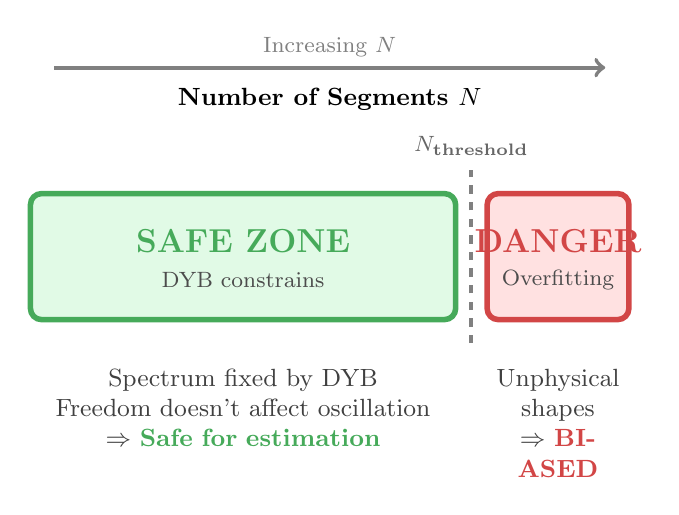
\begin{tikzpicture}[scale=1.0]
  % Define elegant colors
  \definecolor{safegreen}{RGB}{70,170,90}
  \definecolor{dangerred}{RGB}{210,70,70}
  \definecolor{lightsafe}{RGB}{225,250,230}
  \definecolor{lightdanger}{RGB}{255,225,225}

  % Two main zones
  \filldraw[fill=lightsafe, draw=safegreen, line width=2pt, rounded corners=4pt]
    (0,0) rectangle (5.4,1.6);
  \filldraw[fill=lightdanger, draw=dangerred, line width=2pt, rounded corners=4pt]
    (5.8,0) rectangle (7.6,1.6);

  % Zone labels
  \node[font=\large\bfseries, text=safegreen] at (2.7, 1.0) {SAFE ZONE};
  \node[font=\footnotesize, text=black!70] at (2.7, 0.5) {DYB constrains};

  \node[font=\large\bfseries, text=dangerred] at (6.7, 1.0) {DANGER};
  \node[font=\footnotesize, text=black!70] at (6.7, 0.5) {Overfitting};

  % Threshold marker
  \draw[line width=1.5pt, black!50, dashed] (5.6, -0.3) -- (5.6, 1.9);
  \node[font=\footnotesize\bfseries, text=black!60] at (5.6, 2.2) {$N_{\text{threshold}}$};

  % Top labels
  \node[font=\small\bfseries, text=black] at (3.8, 2.8) {Number of Segments $N$};
  \draw[->, line width=1.5pt, black!50] (0.3, 3.2) -- (7.3, 3.2)
    node[midway, above, font=\footnotesize] {Increasing $N$};

  % Bottom annotations
  \node[below=0.5cm of {(2.7,0)}, text width=5.0cm, font=\small, align=center, text=black!75] {
    Spectrum fixed by DYB\\
    Freedom doesn't affect oscillation\\
    $\Rightarrow$ \textcolor{safegreen}{\bfseries Safe for estimation}
  };

  \node[below=0.5cm of {(6.7,0)}, text width=1.7cm, font=\small, align=center, text=black!75] {
    Unphysical\\
    shapes\\
    $\Rightarrow$ \textcolor{dangerred}{\bfseries BIASED}
  };
\end{tikzpicture}
\end{center}

\paragraph{Safe Zone ($N \leq N_{\text{threshold}}$)}
DYB constrains all segments sufficiently that the spectrum shape is essentially fixed for JUNO.
Trade-off within safe zone:
\begin{itemize}
  \item \textbf{Fewer bins ($N$ small):} Larger statistical uncertainty on $\theta$, smaller systematic
  \item \textbf{More bins ($N$ large):} Smaller statistical uncertainty, larger systematic
\end{itemize}

\textbf{Selection principle:} Prefer larger $N$ within the safe zone to minimize model dependence on prior choice.

\paragraph{Dangerous Zone ($N > N_{\text{threshold}}$)}
Too many segments beyond DYB's constraining power. JUNO fit picks unphysical shapes to reduce $\chi^2$,
leading to \textbf{biased oscillation parameters}. Must avoid this regime.

\begin{figure}[h]
  \centering
  \begin{subfigure}[t]{0.45\textwidth}
    \centering
    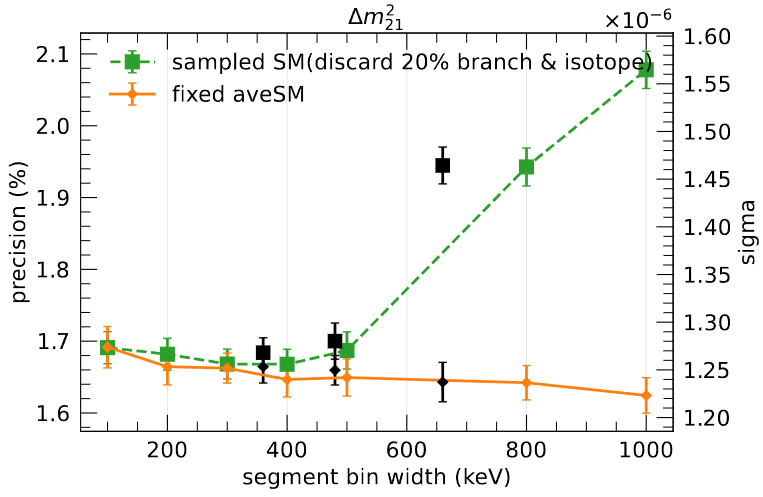
\includegraphics[width=\linewidth]{5_oscillation/segment_dmsq21.png}
    \caption{}
    \label{fig:segment_dmsq21}
  \end{subfigure}
  \hfill
  \begin{subfigure}[t]{0.45\textwidth}
    \centering
    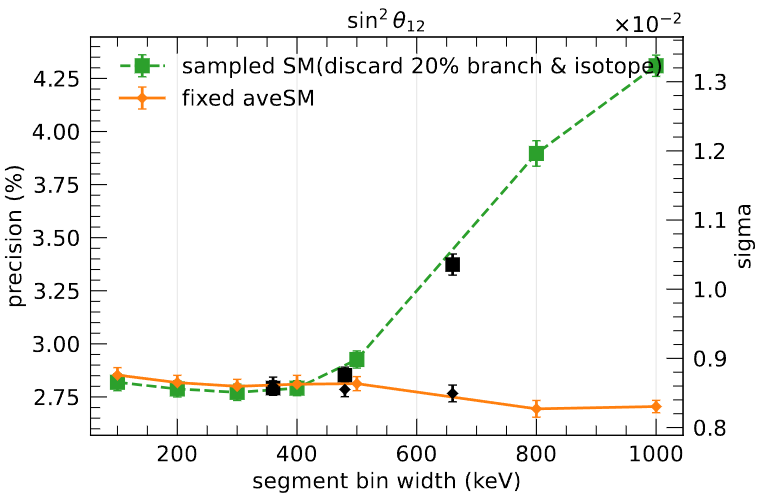
\includegraphics[width=\linewidth]{5_oscillation/segment_sinsq12.png}
    \caption{}
    \label{fig:segment_sinsq12}
  \end{subfigure}
  \caption{Precision of (a) $\Delta m^2_{21}$ and (b) $\sin^2\theta_{12}$ as a function of reactor-spectrum segment width. Green markers/lines show results when the Summation Model is perturbed (randomly discarding 20\% of branches/isotopes); orange markers/lines indicate the baseline precision with a fixed average Summation Model. Black points correspond to segmentation defined by the detector energy resolution (energy-resolution-driven segmentation), while the colored-line points correspond to uniform segmentation of the reactor spectrum. Error bars denote the statistical uncertainty from repeated toys/fits. The additional model-dependent systematic uncertainty is minimized at a segment width of approximately 300\,keV, indicating an optimal trade-off between model flexibility and available statistical constraint.
}
\end{figure}

Figures \ref{fig:segment_dmsq21} and \ref{fig:segment_sinsq12} demonstrate that the additional model-dependent systematic uncertainty is minimized at a segment width of approximately \(300\,\mathrm{keV}\): around this point the difference between the green and orange curves is smallest, indicating effective suppression of model-related uncertainty. Conversely, overly fine segmentation weakens Daya Bay (DYB)'s statistical constraint on each segment and can increase statistical noise or inter-segment correlations, potentially leading to overfitting; overly coarse segmentation cannot absorb local shape differences, causing the model-dependent systematic to grow. Under the perturbation assumptions adopted here, a segment width of about \(300\,\mathrm{keV}\) provides a favorable compromise between reducing model-dependent bias and maintaining adequate statistical constraint.



\subsubsection{Summation Model}

 Currently, the commonly used methods for calculating reactor neutrino flux include the conversion method and the summation method. In recent years, with the continuous improvement and updating of nuclear data, as well as the application of total absorption γ-ray spectroscopy technology, the measurement of β-decay branching data has become more accurate. Consequently, the reliability of neutrino flux models derived via the summation method has been significantly enhanced. The summation method can provide a direct explanation for the reactor neutrino anomaly.

The calculation process of the summation method, as illustrated in the Figure~\ref{fig:summation_procedure}, consists primarily of two components: nuclear database inputs and antineutrino spectra calculation for individual β-decay branches. Further details can be found in Xinzhao’s doctoral dissertation.
 




 \begin{figure}
     \centering
     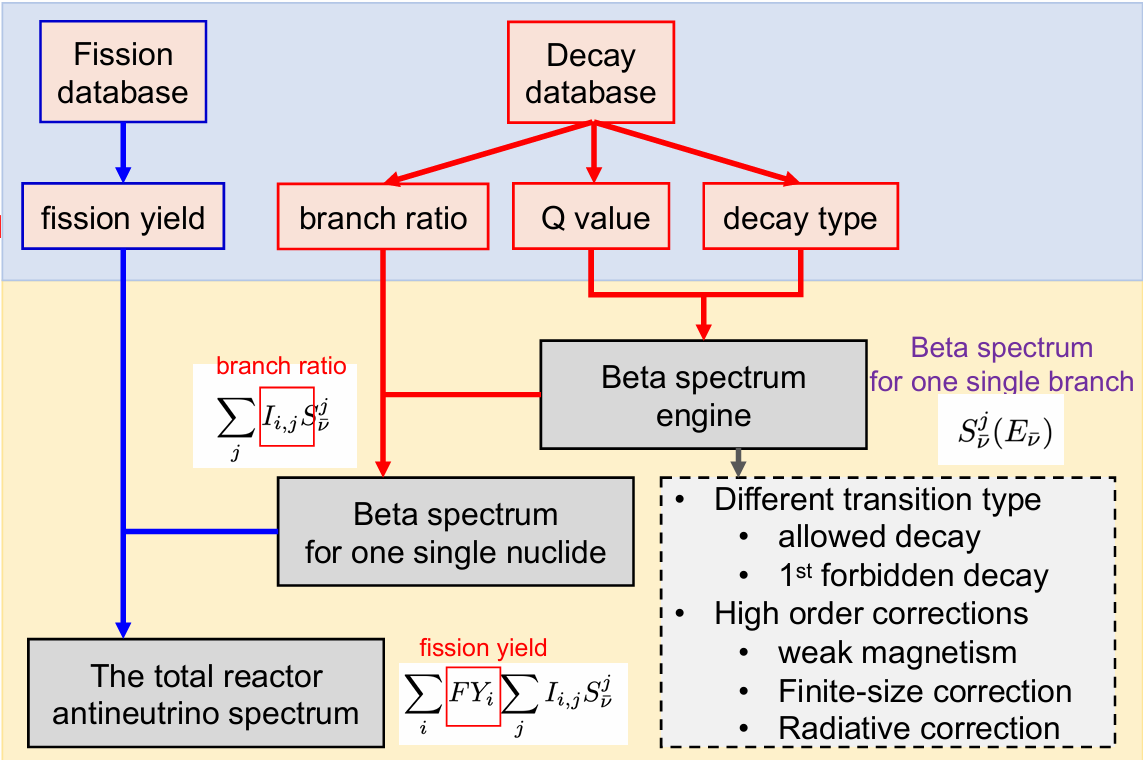
\includegraphics[width=0.75\linewidth]{5_oscillation/summation_procedure.png}
     \caption{Summation spectra calculation framework. The blue region corresponds to the nuclear database inputs, and the yellow region denotes the calculation process of the spectra calculation.}
     \label{fig:summation_procedure}
 \end{figure}

 To investigate the systematic errors in oscillation parameters induced by uncertainties in the shape of the neutrino flux spectrum, it is necessary to construct neutrino spectra with different shapes. This requirement can be achieved by randomly omitting β spectra during the construction of neutrino spectra using the summation method. The specific details are as follows:

\begin{itemize}
  \item Randomly omit $10\% (20\%) $ of the nuclides from all nuclides.
  \item Randomly omit $10\% (20\%) $ the β-decay branches from the remaining nuclides.
  \item Normalize the resulting neutrino spectrum shape to the IBD yield corresponding to the scenario where no nuclides or β-decay branches are omitted.

\end{itemize}

The average spectrum and 1 $\sigma$range of the summation model obtained via the aforementioned method are shown in the Figure~\ref{fig:sm}.
\begin{figure}[htbp] 
    \centering
   
    \begin{subfigure}[t]{0.45\textwidth}
        \centering
        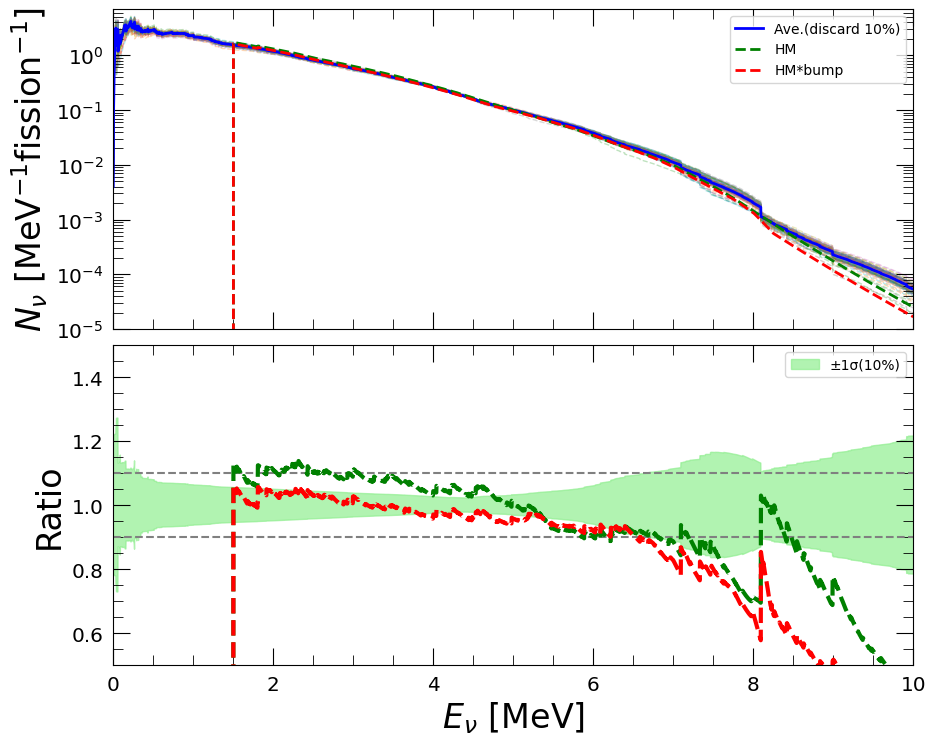
\includegraphics[width=\linewidth]{5_oscillation/sm_discard_0.1.png}
        \caption{Omit 10$\%$} 
        \label{fig:sm_0.1}
    \end{subfigure}
    \hfill  
    \begin{subfigure}[t]{0.45\textwidth}
        \centering
        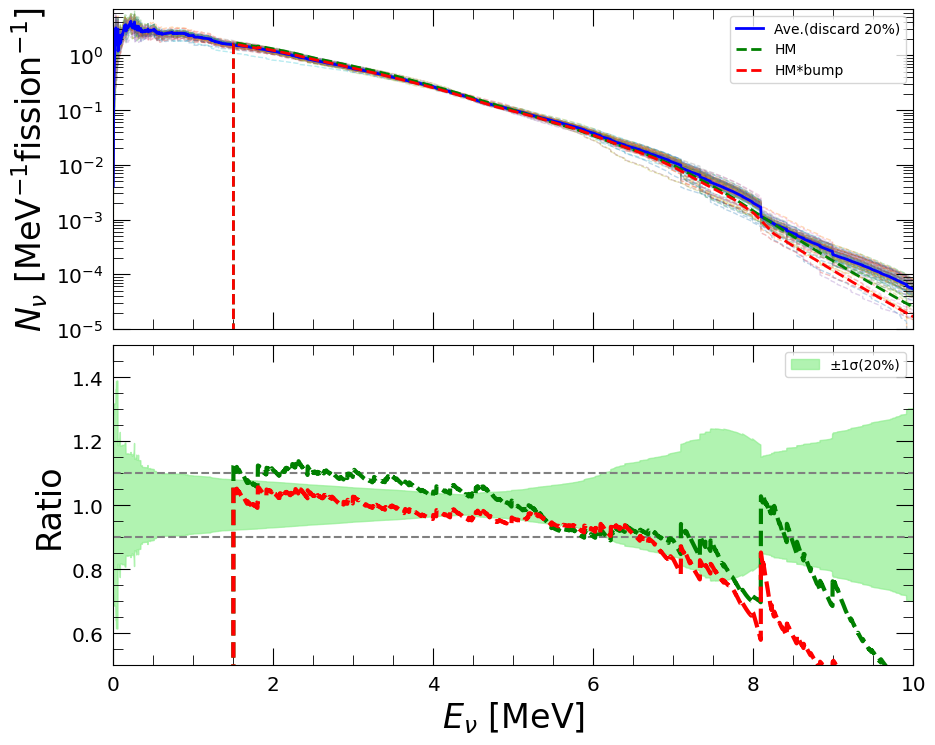
\includegraphics[width=\linewidth]{5_oscillation/sm_0.2.png}
        \caption{Omit 20$\%$}
        \label{fig:sm_0.2}
    \end{subfigure}
    \caption{average spectrum and 1$\sigma$ range of the summation model} 
    \label{fig:sm} 
\end{figure}
\subsection{Feldman-Cousins method}


To validate the use of Wilks' theorem and to obtain confidence intervals with correct coverage in non-regular situations, we performed a series of Feldman--Cousins (FC) coverage studies for the oscillation parameters of interest.  The studies include both a two-dimensional FC construction for the solar-sector parameters and a one-dimensional FC construction for $\Delta m^2_{31}$.

\subsubsection{2D Feldman--Cousins for \(\Delta m^2_{21}\) and \(\sin^2\theta_{12}\)}
We constructed an empirical distribution of the test statistic
\[
\Delta\chi^2(\delta) \equiv \chi^2(\delta) - \chi^2_{\min},
\]
by generating ensembles of pseudo-experiments (toys) under the nominal hypothesis and refitting each toy according to the standard Feldman--Cousins (FC) prescription. For the two-dimensional parameter space \((\Delta m^2_{21},\,\sin^2\theta_{12})\), the expected asymptotic behaviour of the test statistic follows a $\chi^2$ distribution with two degrees of freedom.

Figure~\ref{fig:FC21} shows the empirical $\Delta\chi^2$ distribution obtained at a representative grid point in the \((\Delta m^2_{21},\,\sin^2\theta_{12})\) plane. The extracted critical value at 68.27\% C.L.\ is consistent with the Wilks expectation within statistical uncertainties. Therefore, for the solar-sector parameters \((\Delta m^2_{21},\sin^2\theta_{12})\), the Wilks approximation is adequate in the tested region.

\begin{figure}[h]
    \centering
    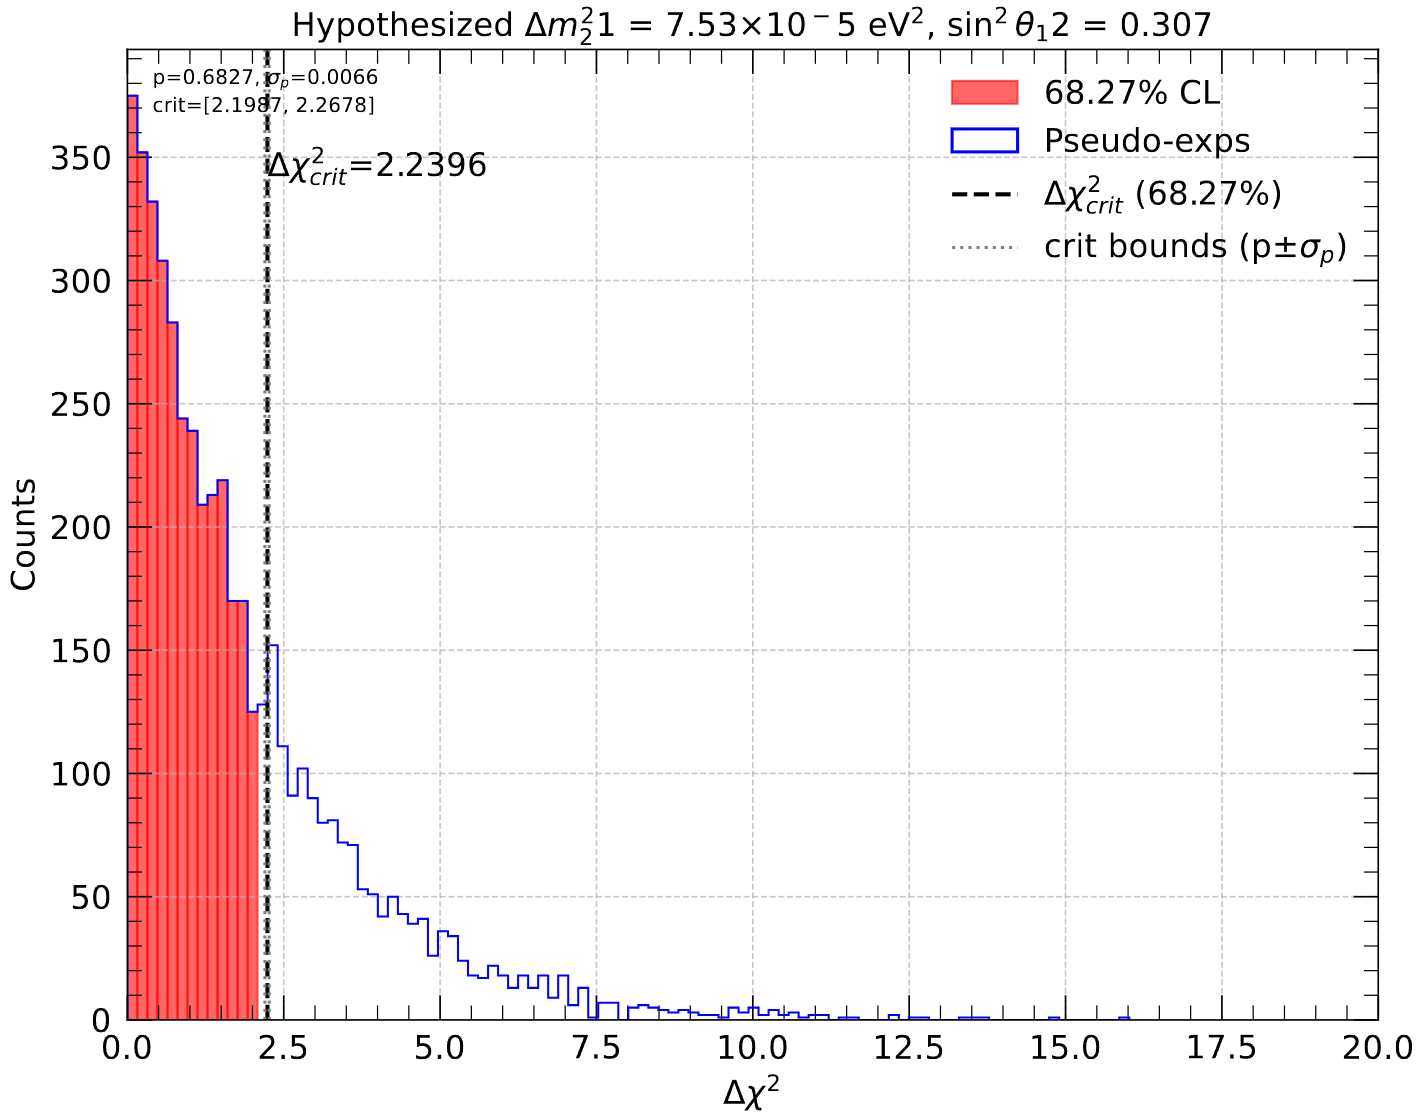
\includegraphics[width=0.7\linewidth]{5_oscillation/FC21.png}
    \caption{Empirical $\Delta\chi^2$ distribution from the 2D Feldman--Cousins test at a representative point in the \((\Delta m^2_{21},\,\sin^2\theta_{12})\) parameter space. The vertical dashed line indicates the critical value at 68.27\% C.L., which agrees with the Wilks expectation of a two-degrees-of-freedom $\chi^2$ distribution.}
    \label{fig:FC21}
\end{figure}


\subsubsection{1D Feldman--Cousins for \(\Delta m^2_{31}\)}
By contrast, the likelihood surface for \(\Delta m^2_{31}\) exhibits non-regular behaviour (nearby unphysical minima and phase-degeneracy effects) that invalidates the naive Wilks approximation in the JUNO-only configuration. We therefore applied a one-dimensional FC construction for \(\Delta m^2_{31}\). The FC procedure was carried out in two steps to assess the impact of reactor-spectrum model uncertainty:

\begin{enumerate}
  \item \textbf{Fixed reactor model:} With the reactor spectrum fixed to the average Summation Model (no shape perturbation), we generated toy ensembles and computed the empirical distribution of $\Delta\chi^2$. The resulting critical value for the 68.27\% acceptance region is
  \[
    \Delta\chi^2_{\rm crit,\,fixed} = 1.5379,
  \]
  which yields a \(\Delta m^2_{31}\) precision of \(1.39\%\) (for the 50-day exposure). The distribution of per-toy precision for this fixed-model case is shown in Fig.~\ref{fig:dmsq31_fixedaveSM}.
  \item \textbf{Sampled reactor model:} To include reactor-model variation we sampled an ensemble of perturbed reactor spectra by varying each 20-keV segment (the sampled-model ensemble, $N_{\rm toys}=5000$), and repeated the FC construction using these perturbed models. The empirical critical value becomes
  \[
    \Delta\chi^2_{\rm crit,\,sampled} = 1.5724,
  \]
  corresponding to a \(\Delta m^2_{31}\) precision of \(1.40\%\) (50-day exposure). The per-toy precision distribution for the sampled (Gaussian-perturbed) models is shown in Fig.~\ref{fig:dmsq31_gaussian}.
\end{enumerate}

The critical value increases slightly when using the sampled reactor-model ensemble compared to the fixed model. The observed difference is small; moreover, the uncertainty on the empirical critical values can be reduced further by increasing the number of toys in the FC ensembles.

From the above studies we draw the following conclusions:
\begin{itemize}
  \item The model-dependent systematic uncertainty affecting \(\Delta m^2_{31}\) is small: we estimate the additional systematic contribution from reactor-model variation to be \(<0.3\%\) on the \(\Delta m^2_{31}\) precision in the 50-day scenario.
  \item For all three parameters considered (\(\Delta m^2_{21}\), \(\sin^2\theta_{12}\), and \(\Delta m^2_{31}\)), the systematic uncertainty induced by realistic reactor-model variations is smaller than the statistical uncertainty for the 50-day exposure; i.e., the remaining model-dependent systematics are negligible at this exposure.
  \item The FC-derived precision for \(\Delta m^2_{31}\) under the adopted assumptions is \(\approx 1.4\%\) (50-days exposure). This is slightly worse than the global-fit precision (approximately \(1.1\%\)) but is internally consistent given the JUNO-only configuration and the treated reactor-model uncertainties.
\end{itemize}

\paragraph{Practical notes.} The FC ensembles reported above used $N_{\rm toys}=5000$ pseudo-experiments for the sampled-model case; increasing $N_{\rm toys}$ will reduce the statistical uncertainty on the empirical critical $\Delta\chi^2$ values. The FC procedure and the quoted numbers should therefore be interpreted with their toy-statistics uncertainty in mind.

\begin{figure}[!htbp]
  \centering
  \begin{subfigure}[t]{0.45\textwidth}
    \centering
    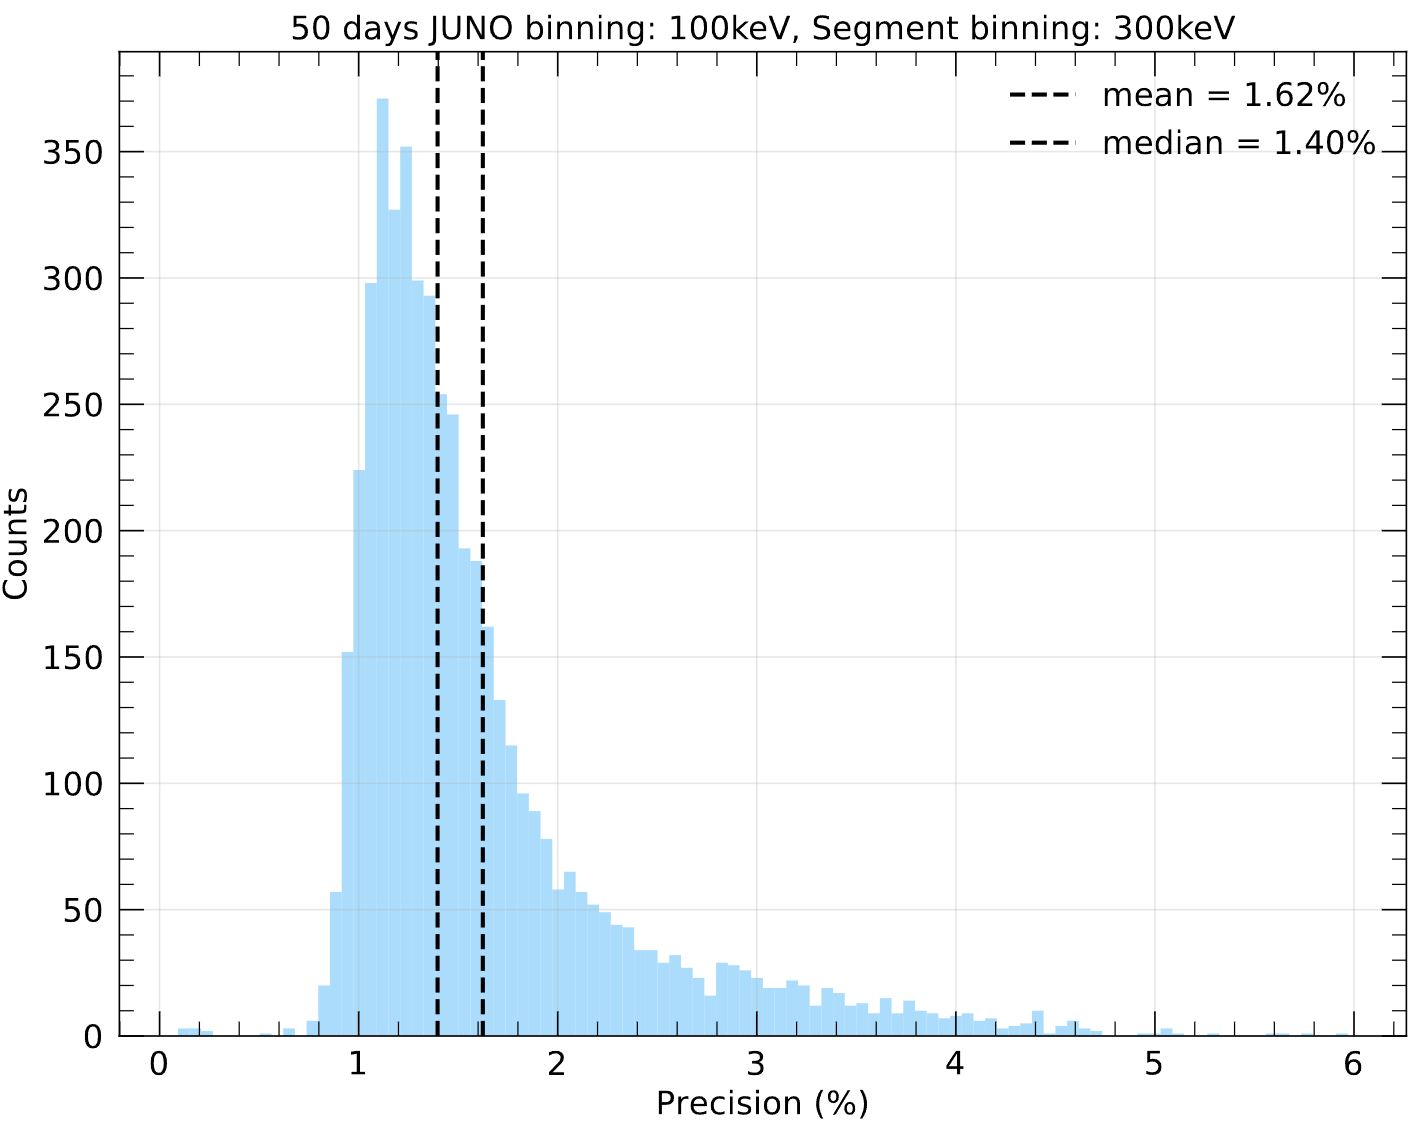
\includegraphics[width=\linewidth]{5_oscillation/dmsq31_gaussian.png}
    \caption{Per-toy precision distribution for the sampled (Gaussian-perturbed) reactor-model ensemble ($N_{\rm toys}=5000$).}
    \label{fig:dmsq31_gaussian}
  \end{subfigure}%
  \hfill
  \begin{subfigure}[t]{0.45\textwidth}
    \centering
    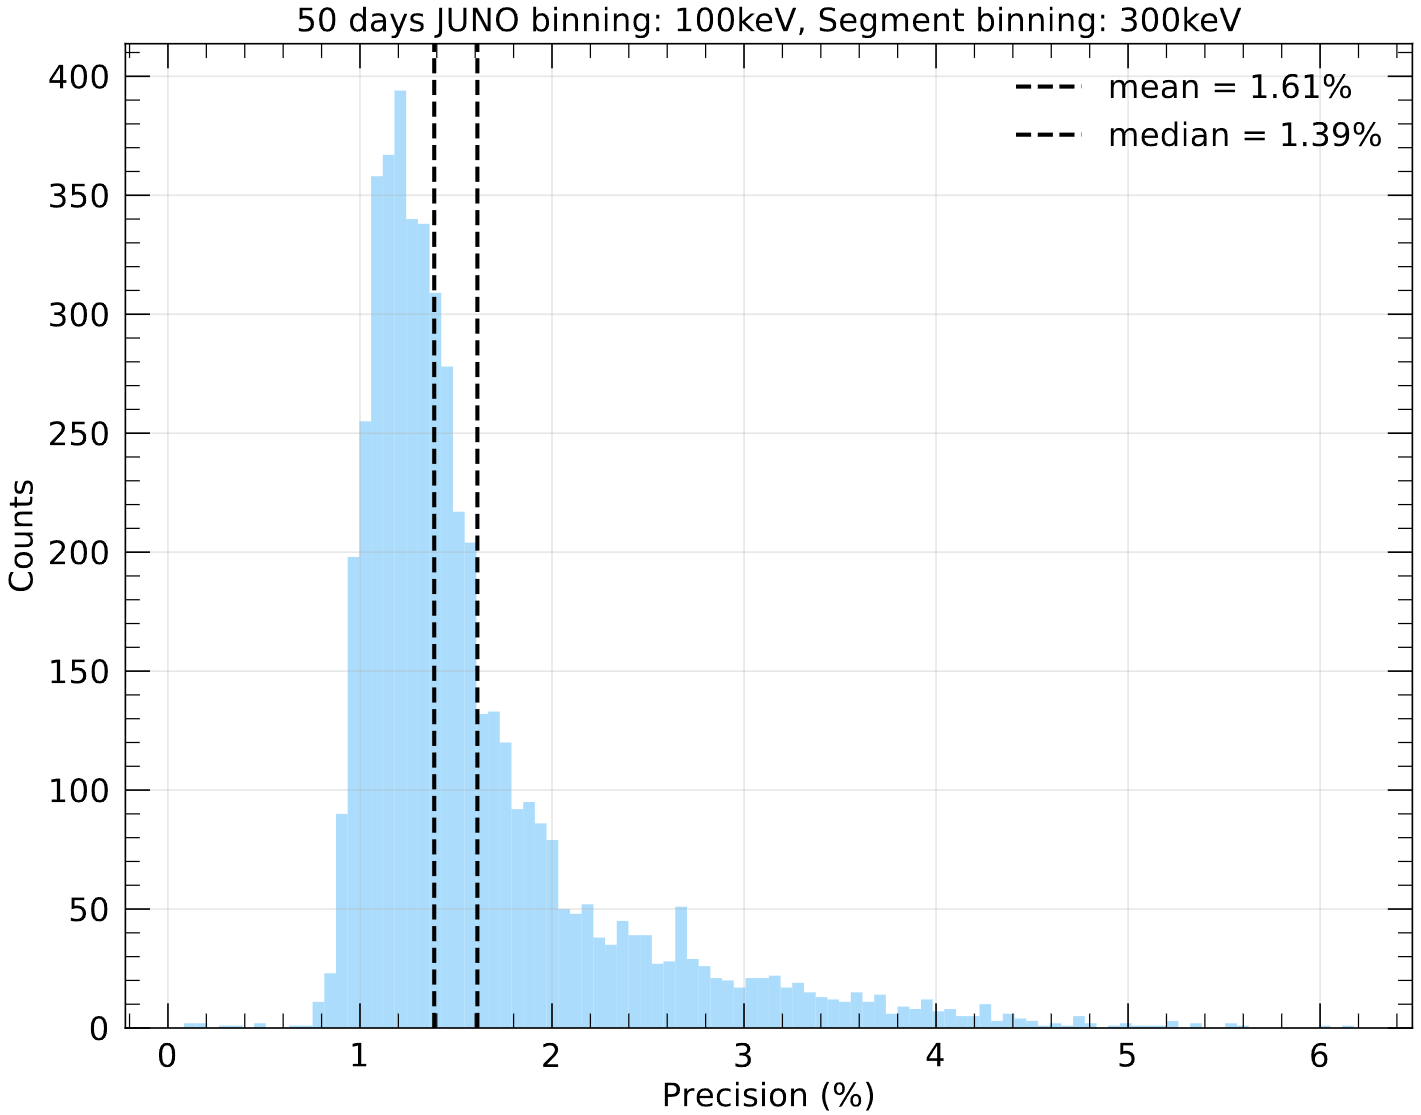
\includegraphics[width=\linewidth]{5_oscillation/dmsq31_fixedaveSM.png}
    \caption{Per-toy precision distribution for the fixed average Summation Model ($N_{\rm toys}=5000$) (no shape perturbation).}
    \label{fig:dmsq31_fixedaveSM}
  \end{subfigure}
  \label{fig:dmsq31_FC}
\end{figure}

\subsection{Oscillation analysis result}
\label{subsec:analysis:result}
Incorporating the estimates of selection efficiency, background contributions, and reactor information, the observed prompt energy spectrum of IBD candidates shown in Fig.~\ref{fig:P25C:spectrum} is compared with a detailed prediction to extract the neutrino oscillation parameters. The spectral distortion observed in the prompt-energy spectrum in Fig.~\ref{fig:P25C:spectrum} was primarily shaped by solar oscillation parameters $\Delta m_{21}^2$ and $\sin^2\theta_{12}$. 
Given the limited statistics of the current data, $\rm{sin}^2\theta_{13}=0$ cannot be strongly rejected in JUNO. However, the third oscillation pattern has already been firmly established by the Daya Bay measurements with high significance. Therefore, external constraints on $\rm{sin}^2\theta_{13}$ and $\Delta m^2_{31}$ from Daya Bay are applied by default. We find that applying or removing the $\Delta m^2_{31}$ constraint has a negligible impact on the measurement of the solar oscillation parameters $\sin^2\theta_{12}$ and $\Delta m^2_{21}$, the measurement is insensitive to the neutrino mass ordering. Due to the currently limited statistics, our oscillation analysis concentrated on determining the solar parameters. The residuals between data and the full prediction are small and consistent within 2$\sigma$, yielding a goodness of fit of $\chi^2/\rm{ndf}=63.03/64$.

\begin{figure}[!htbp]
    \centering
    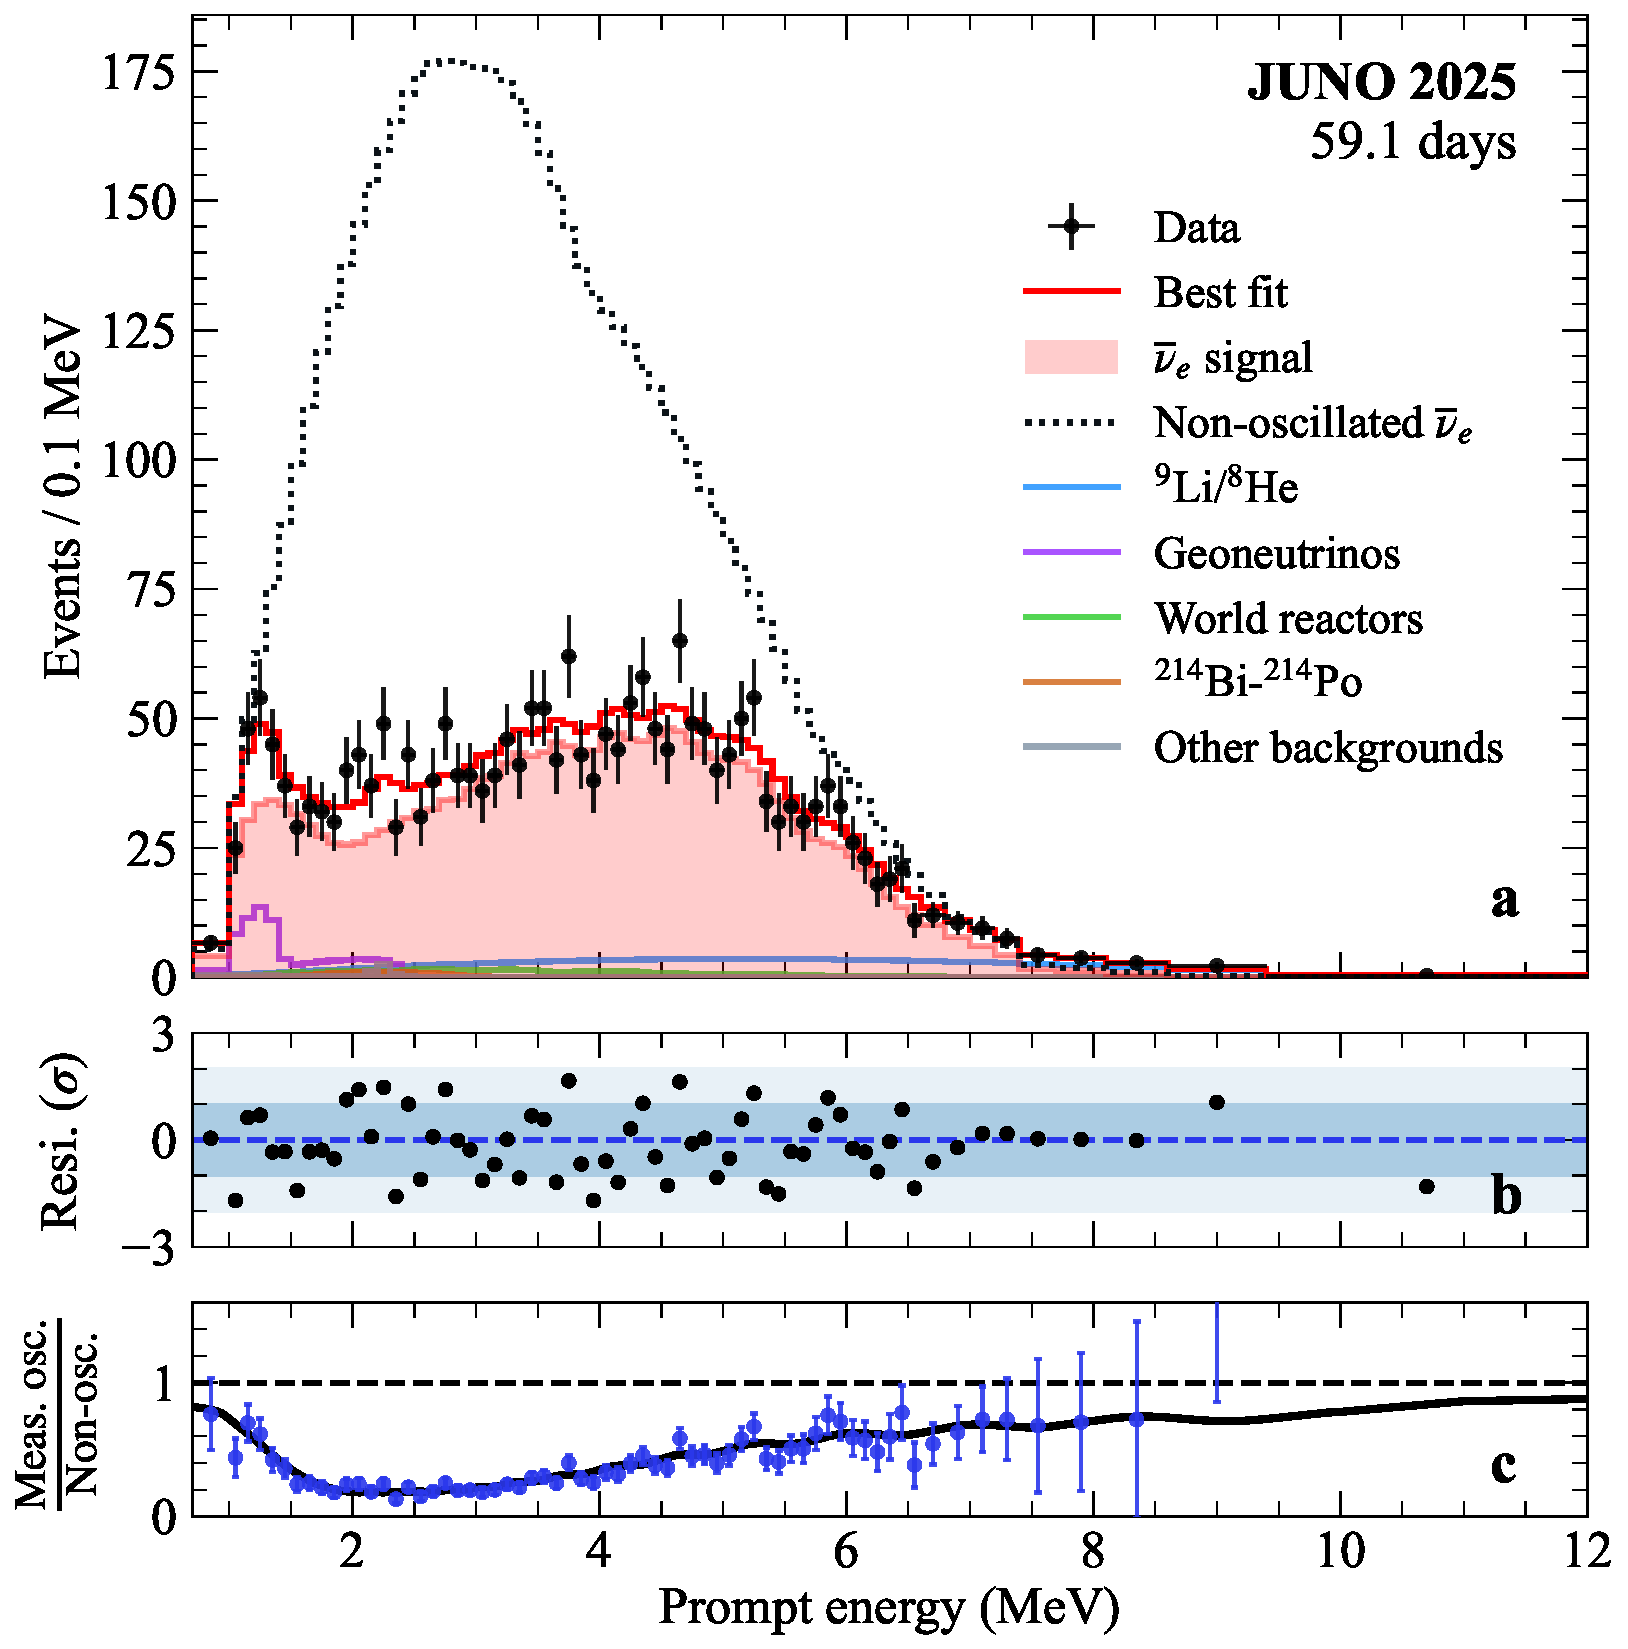
\includegraphics[width=0.65\linewidth]{5_oscillation/spectrum_component_v3.2.pdf}
    \caption{Measured energy spectrum of prompt IBD candidates. a, Black points show measured data with statistical error bars, with the red curve indicating the best-fit oscillation model. Shaded red region represents expected antineutrino signal. Black dotted line represents non-oscillated reactor neutrino expectation. Backgrounds are indicated by other solid color lines. b, Residuals quantifying the statistical consistency between data and the complete model. c, Ratio of the measured oscillated spectrum to non-oscillated prediction.}
    \label{fig:P25C:spectrum}
\end{figure}

The oscillation analysis yielded the following results for the solar parameters for normal mass ordering scenario:
\begin{equation}
\sin^2\theta_{12} &= 0.3092 \pm 0.0087 ,~~~
\Delta m_{21}^2 &= (7.50 \pm 0.12) \times 10^{-5}~\mathrm{eV}^2 .
\end{equation}
The fraction of neutron capture on carbon (99.22\%) is not included in this analysis, but it has a negligible impact on both the best-fit oscillation parameters and their precision.
The allowed regions of oscillation parameters are shown in Fig.~\ref{fig:P25C:osci}. Results from other measurements of reactor neutrinos (KamLAND~\cite{gando2013reactor} and SNO+~\cite{abreu2025measurement}) and solar neutrinos (combined Super-Kamiokande (SK)+SNO~\cite{abe2024solar}) are also shown for comparison in Fig.~\ref{fig:P25C:osci} and Fig.~\ref{fig:P25C:GlobalComp}. This result improved the precision of both parameters by a factor of 1.6.

\begin{figure}[htbp]
    \centering
    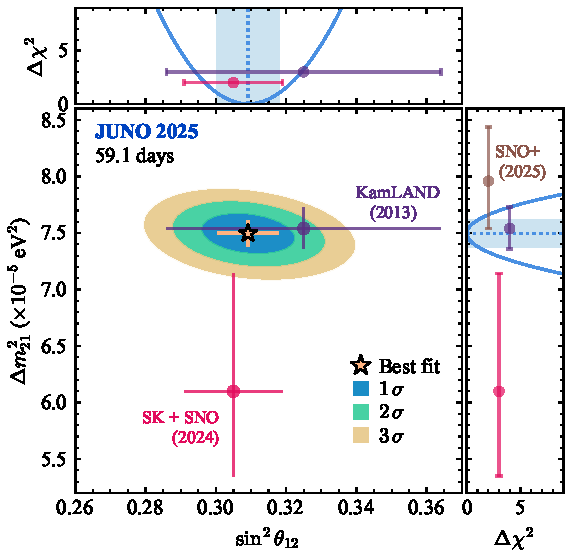
\includegraphics[width=0.65\linewidth]{5_oscillation/plot_contour_sinsq12_dmsq21_with_profiles_NO_errorbar_otherexp_v3.pdf}
    \caption{Results on solar oscillation parameters. Confidence intervals of $\sin^2\theta_{12}$ and $\Delta m_{21}^2$ obtained from the spectral fit of the prompt antineutrino energy spectrum in Fig.~\ref{fig:P25C:spectrum}. Shaded elliptical regions denote the $1\sigma$, $2\sigma$, and $3\sigma$ confidence levels ($\Delta\chi^2 = 2.30,\ 6.18,\ 11.83$). The upper panel shows the one-dimensional $\Delta\chi^2$ for $\sin^2\theta_{12}$ with $\Delta m_{21}^2$ profiled; the right panel shows the corresponding result for $\Delta m_{21}^2$ with $\sin^2\theta_{12}$ profiled. The star indicates the JUNO best-fit point, and the error bars represent the one-dimensional $1\sigma$ intervals.}
    \label{fig:P25C:osci}
\end{figure}

\begin{figure}[!htbp]
  \centering
  \begin{subfigure}[t]{0.45\textwidth}
    \centering
    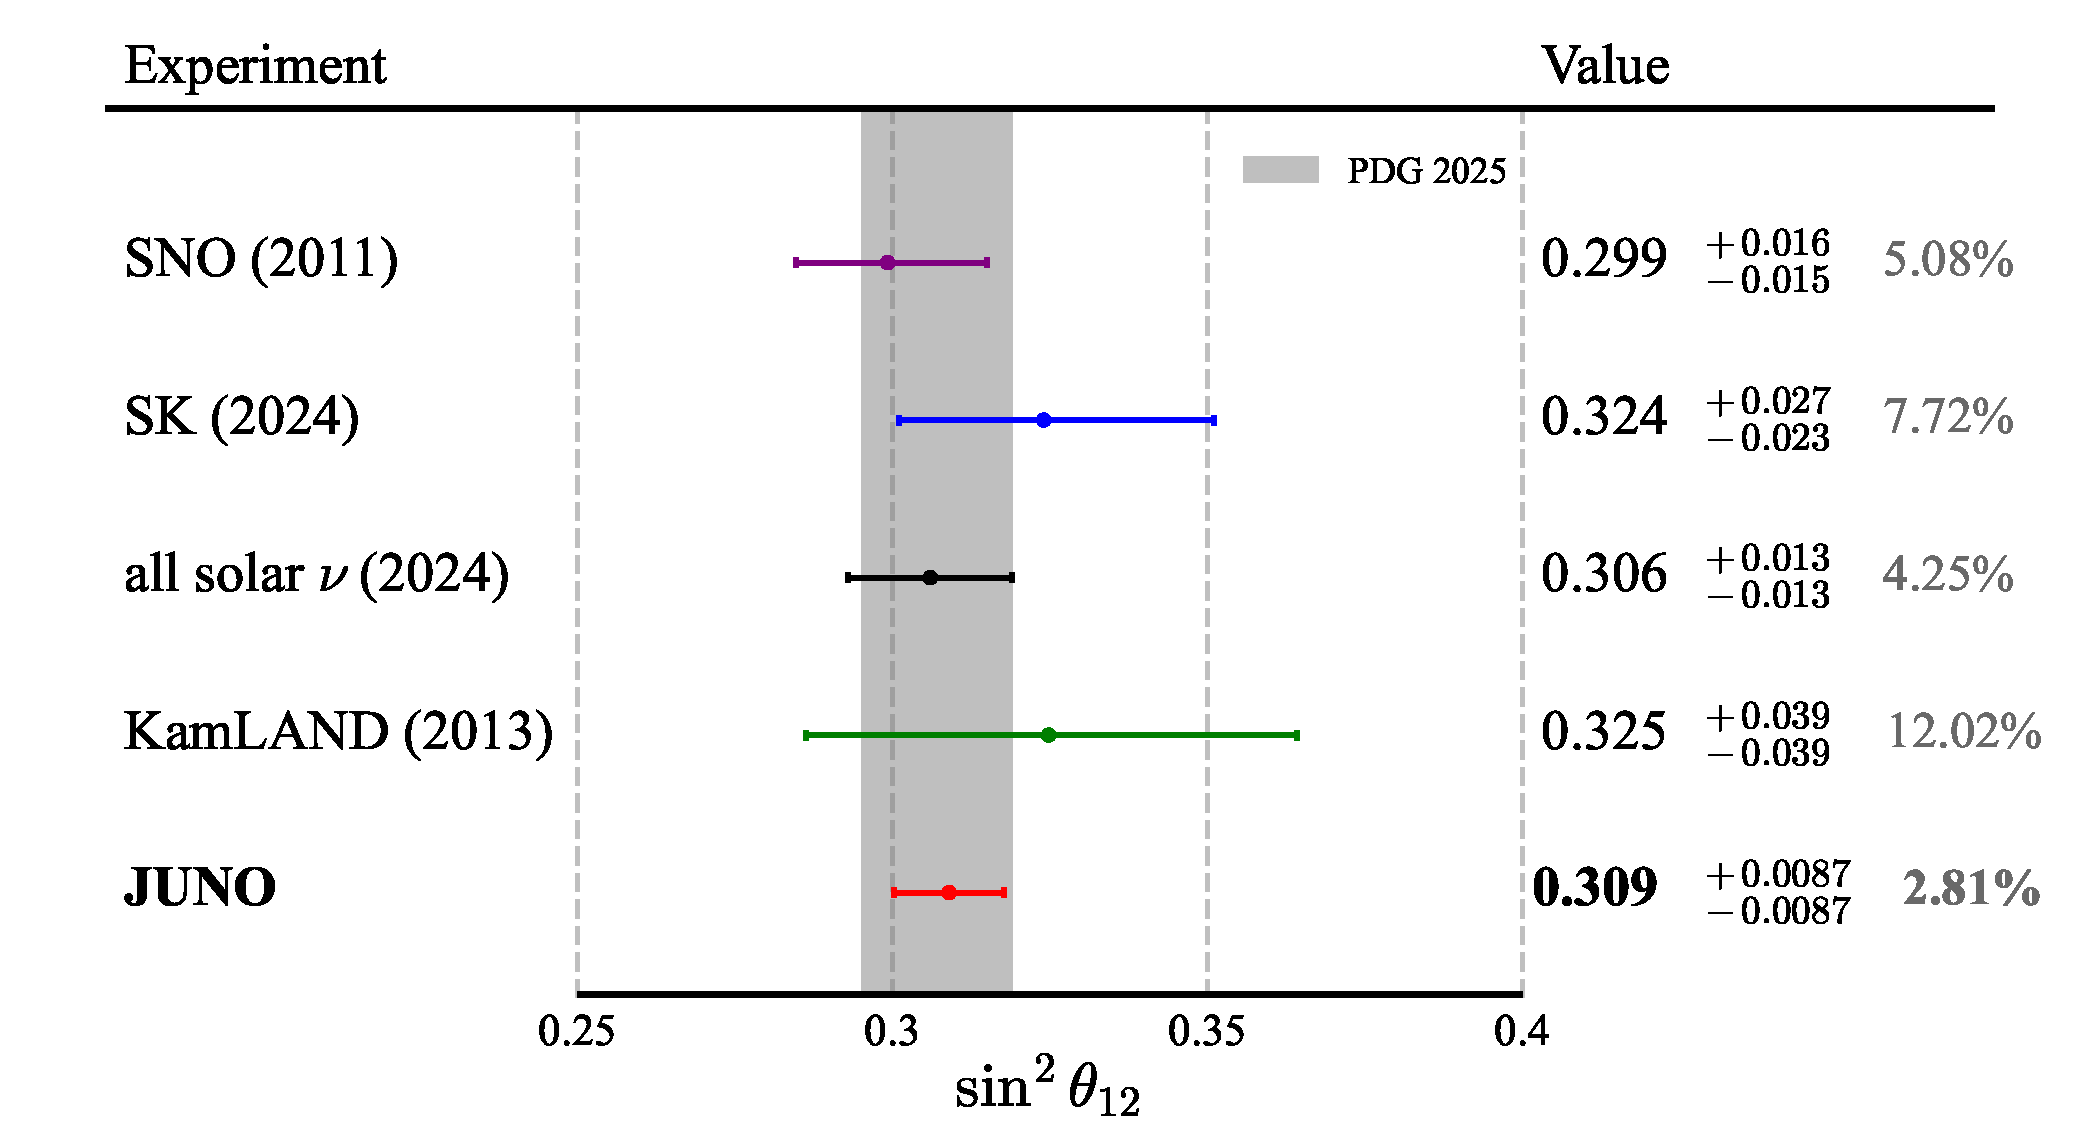
\includegraphics[width=\linewidth]{5_oscillation/th12_new_v251119_w_all_solar.pdf}
    \caption{}
    \label{fig:GlobalComp_sinsq12}
  \end{subfigure}%
  \hspace{0.02\textwidth}
  \begin{subfigure}[t]{0.45\textwidth}
    \centering
    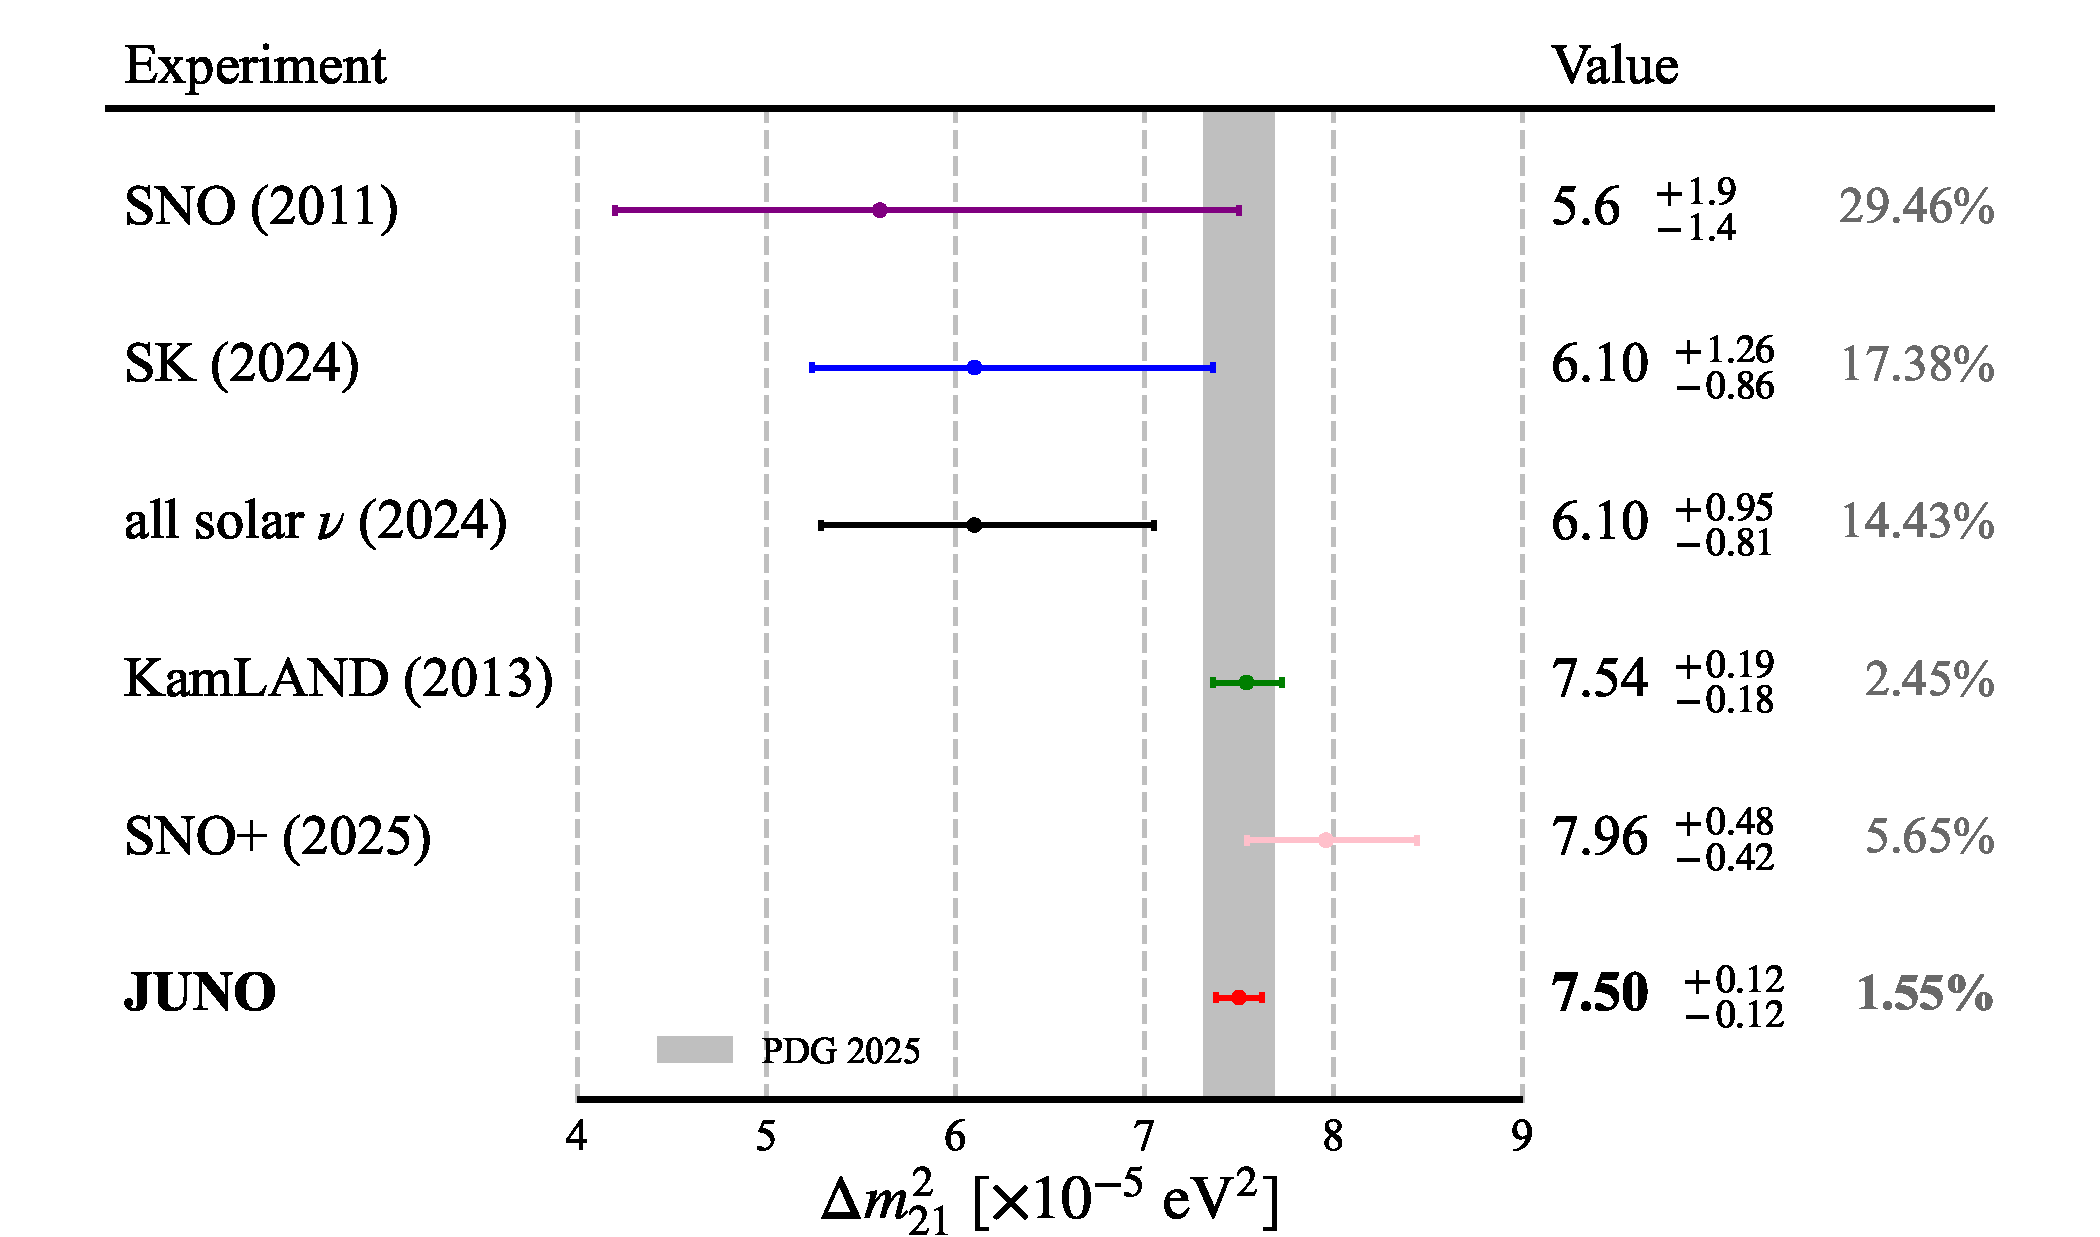
\includegraphics[width=\linewidth]{5_oscillation/m21_v251119_sno+_prl_w_all_solar.pdf}
    \caption{}
    \label{fig:GlobalComp_dmsq21}
  \end{subfigure}
  \caption{Global comparisons of $\sin^2\theta_{12}$ and $\Delta m_{21}^2$ between JUNO and other experiments, together with the PDG 2025 values, are shown in Fig.~\ref{fig:GlobalComp_sinsq12} and Fig.~\ref{fig:GlobalComp_dmsq21}, respectively.}
  \label{fig:P25C:GlobalComp}
\end{figure}

The resulting time evolution of the predicted IBD rate, compared to the measured rate with backgrounds subtracted, is shown in Fig.~\ref{fig:P25C:rate_time_evolution}; the observed variations closely track the known reactor power history. 
% To clearly illustrate the oscillation pattern, we compute the preliminary $L_{\rm eff}/E_\nu$ spectrum shown in Fig.~\ref{fig:P25C:LOverE}, where $L_{\rm eff}$ denotes the flux-weighted baseline of the YJ and TS reactor cores, and the neutrino energy is approximated as $E_\nu \approx E_{\rm rec}+0.784~\rm{MeV}$. The data points are consistent with the predicted oscillation probability, except for the point at large $L/E$, which corresponds to a reconstructed energy of around 3 MeV. The origin of this deviation is under investigation.
\begin{figure}[htbp]
    \centering
    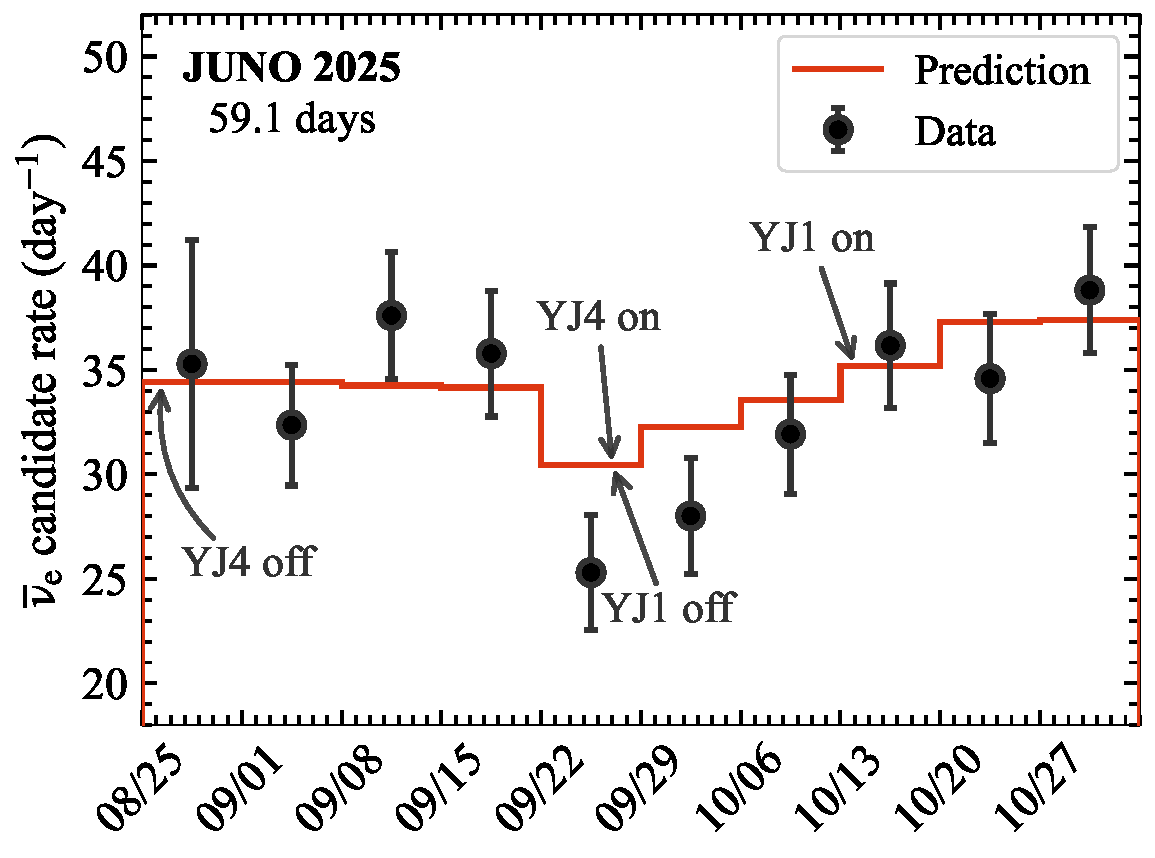
\includegraphics[width=0.65\linewidth]{5_oscillation/IBD_rate_time_evolution.pdf}
    \caption{Temporal distribution of reactor neutrinos. Rates of antineutrino candidates (after subtraction of the mean background rates), shown in one-week time bins (black points with statistical error) are compared to the prediction (red line). Arrows indicate operations on the cores YJ1 and YJ4 of the Yangjiang NPP. The NPP reduced the power output due to the occurrence}
    \label{fig:P25C:rate_time_evolution}
\end{figure}

% \begin{figure}[!htbp]
%     \centering
%     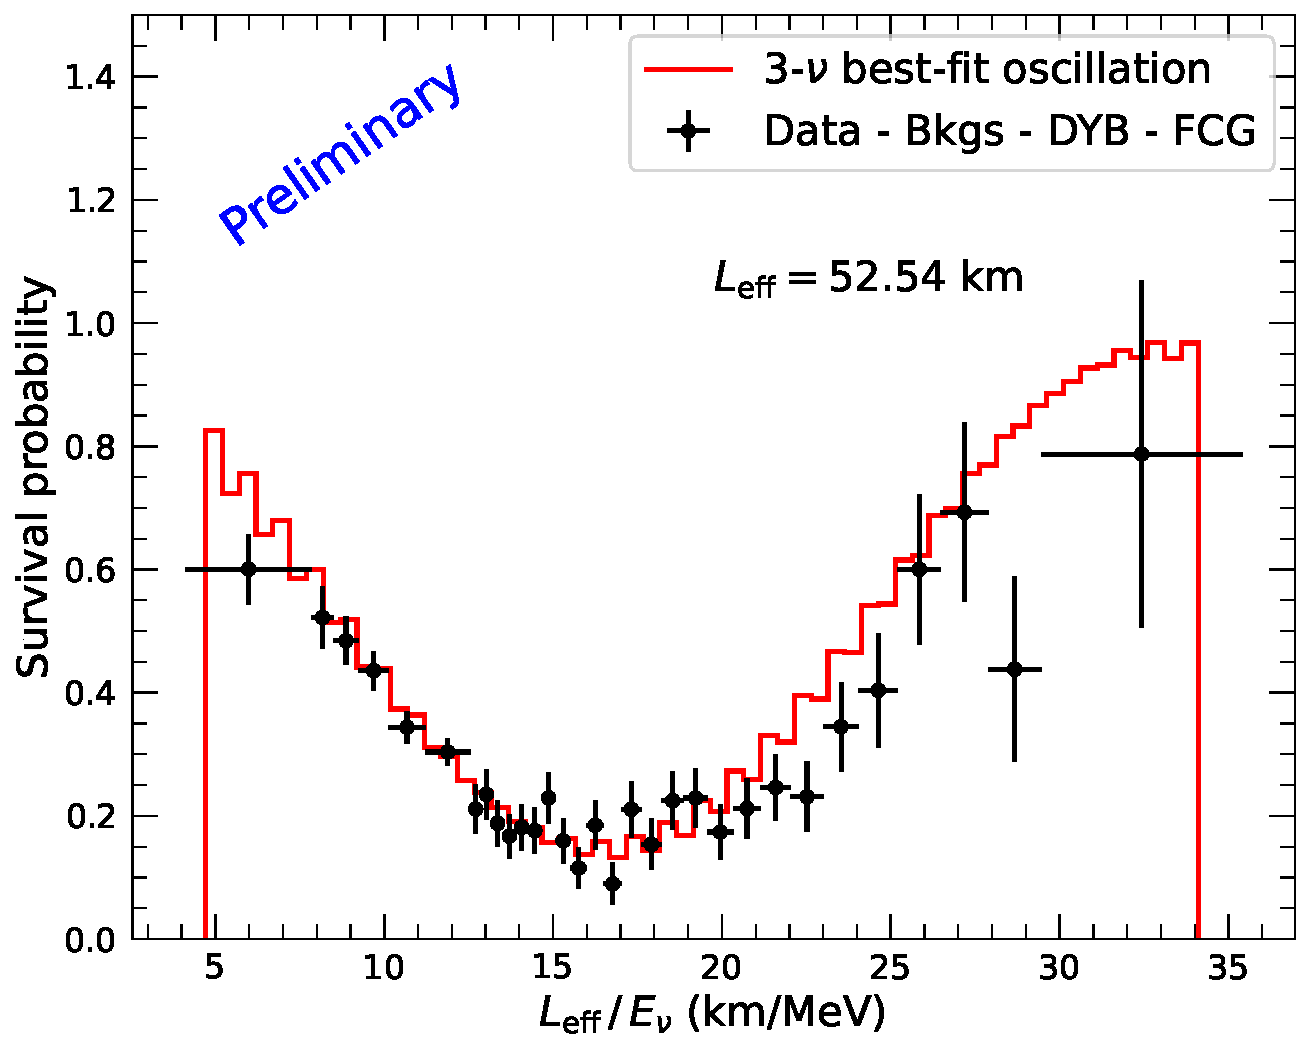
\includegraphics[width=0.65\linewidth]{5_oscillation/Leff_over_Enu_spec.pdf}
%     \caption{Measured $L/E$ spectrum of prompt IBD candidates from the YJ and TS reactor cores. Backgrounds and the IBD contributions from DYB and FCG have been subtracted. The red curve shows the expected three-neutrino survival probability calculated with the best-fit oscillation parameters.}
%     \label{fig:P25C:LOverE}
% \end{figure}

% \subsection{Error budget}

% \begin{figure}[h]
%   \centering
%   \begin{subfigure}[t]{0.32\textwidth}
%     \centering
%     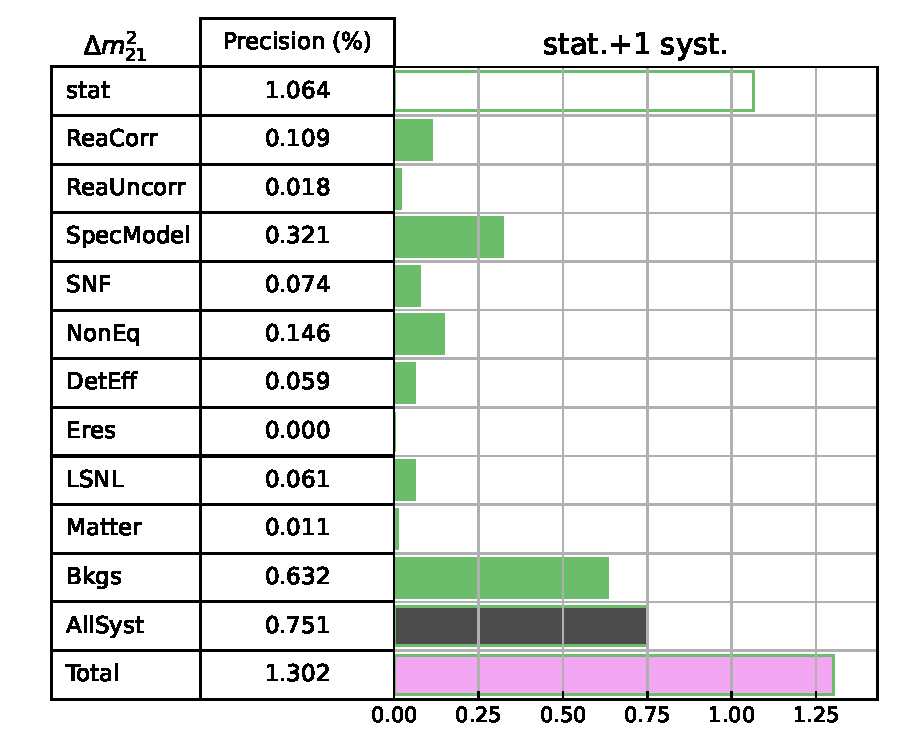
\includegraphics[width=\linewidth]{5_oscillation/dmsq21_50ds_juno_only.pdf}
%     \caption{50 days}
%     \label{fig:l1}
%   \end{subfigure}
%   \hfill
%   \begin{subfigure}[t]{0.32\textwidth}
%     \centering
%     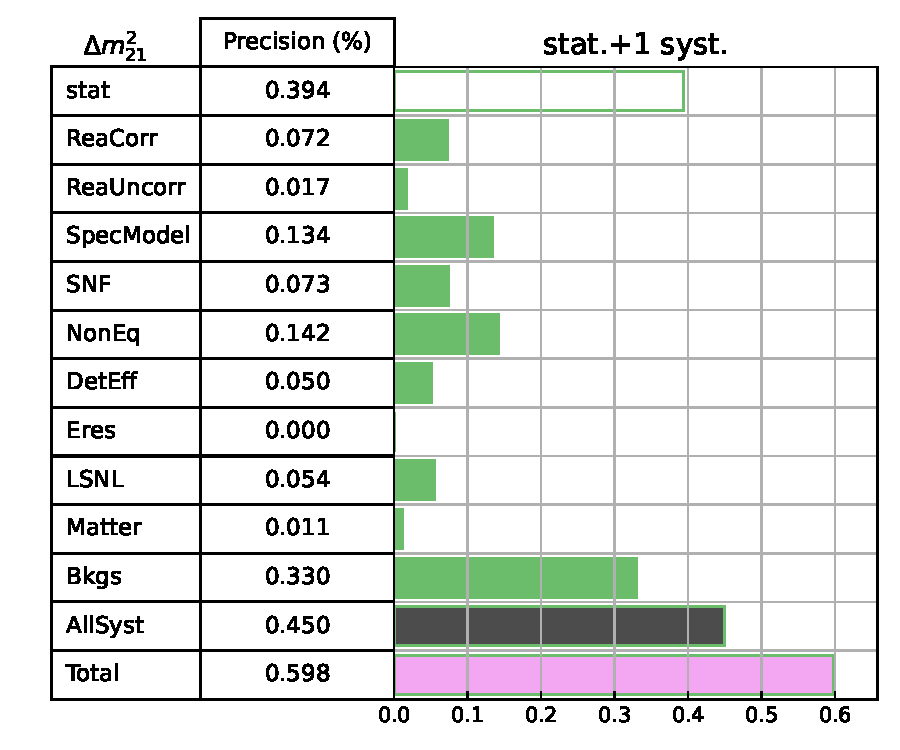
\includegraphics[width=\linewidth]{5_oscillation/dmsq21_1yr_juno_only.pdf}
%     \caption{1 year}
%     \label{fig:l2}
%   \end{subfigure}
%   \hfill
%   \begin{subfigure}[t]{0.32\textwidth}
%     \centering
%     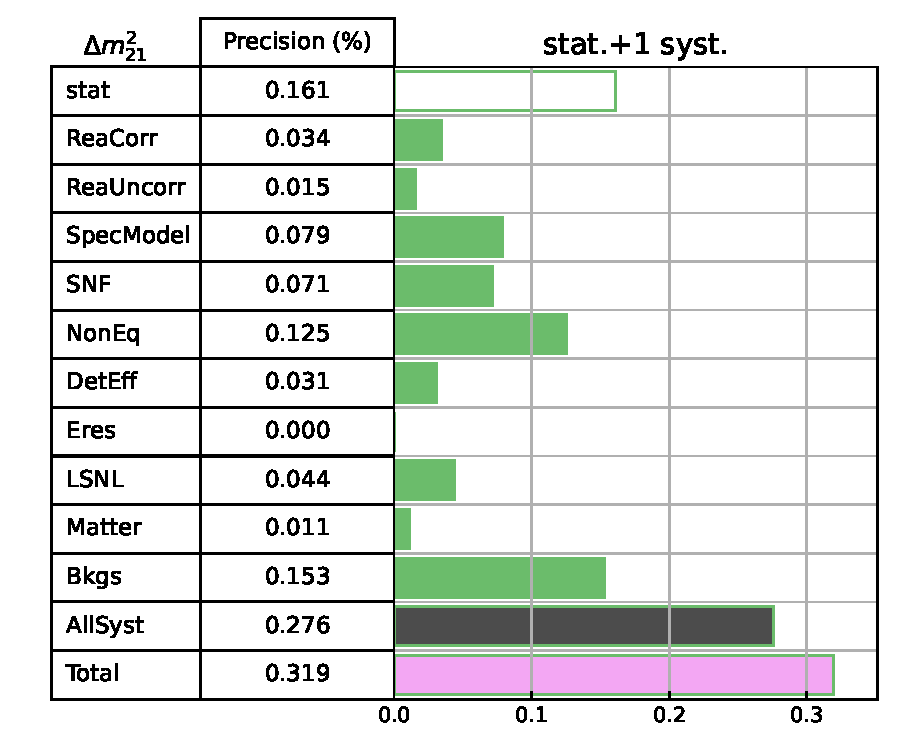
\includegraphics[width=\linewidth]{5_oscillation/dmsq21_6yr_juno_only.pdf}
%     \caption{6 years}
%     \label{fig:l3}
%   \end{subfigure}
%   \caption{Precision breakdown of $\rm \Delta m^2_{21}$}
%   %\label{Precision breakdown of $\rm \Delta m^2_{21}$}
% \end{figure}

% \begin{figure}[h]
%   \centering
%   \begin{subfigure}[t]{0.32\textwidth}
%     \centering
%     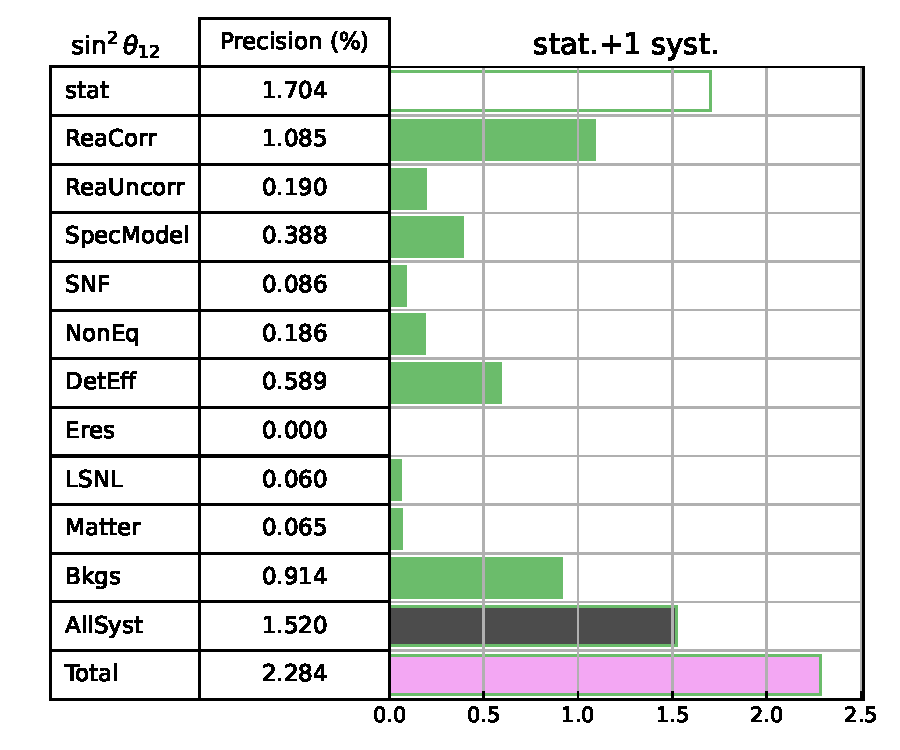
\includegraphics[width=\linewidth]{5_oscillation/sinsq12_50ds_juno_only.pdf}
%     \caption{50 days}
%     \label{fig:l1}
%   \end{subfigure}
%   \hfill
%   \begin{subfigure}[t]{0.32\textwidth}
%     \centering
%     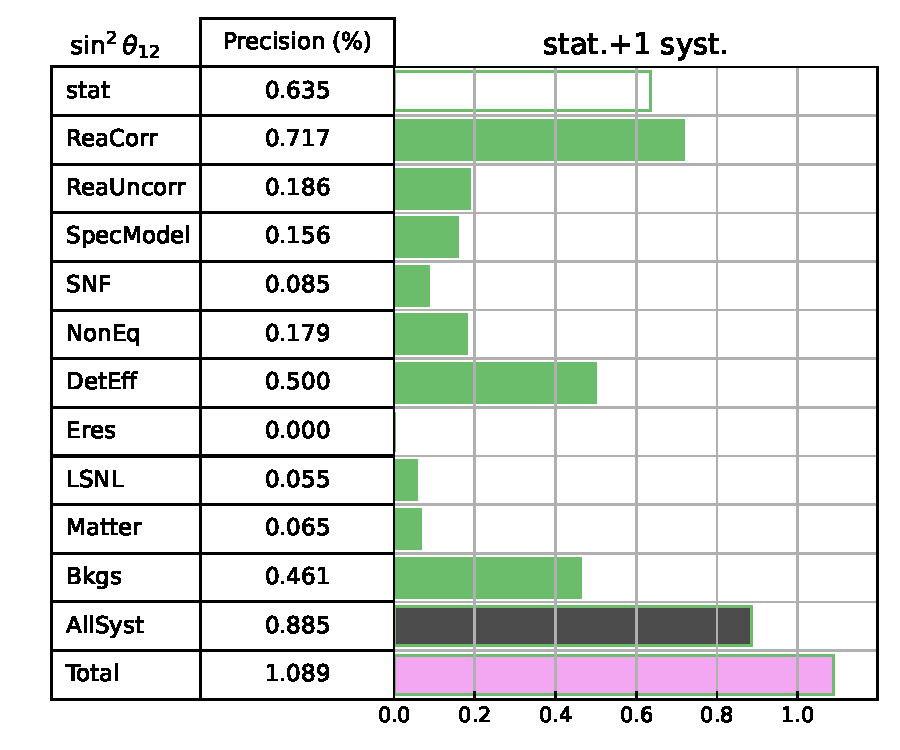
\includegraphics[width=\linewidth]{5_oscillation/sinsq12_1yr_juno_only.pdf}
%     \caption{1 year}
%     \label{fig:l2}
%   \end{subfigure}
%   \hfill
%   \begin{subfigure}[t]{0.32\textwidth}
%     \centering
%     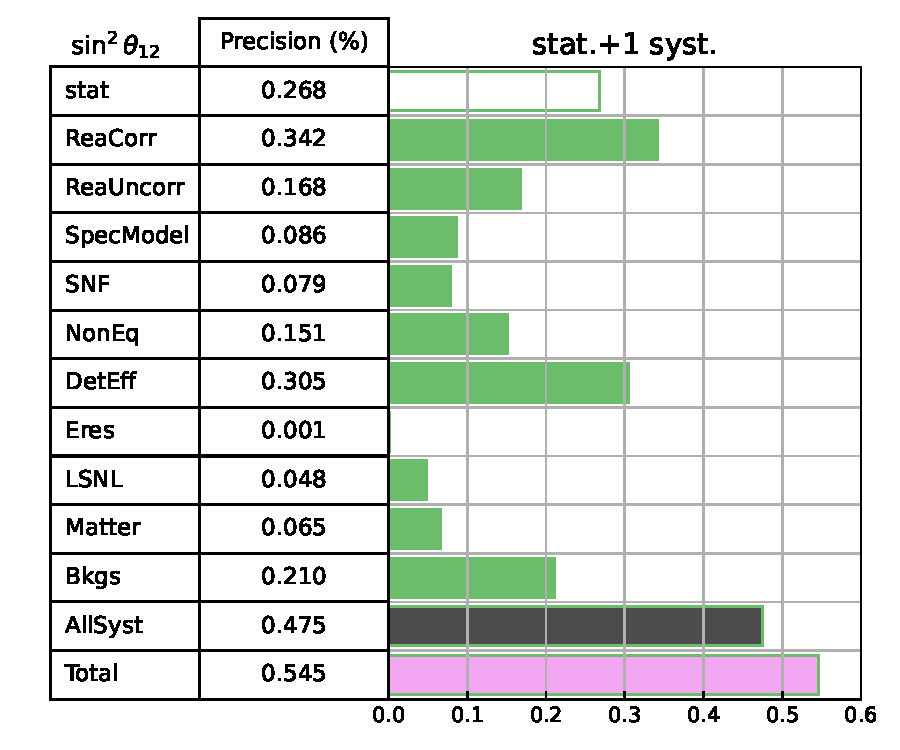
\includegraphics[width=\linewidth]{5_oscillation/sinsq12_6yr_juno_only.pdf}
%     \caption{6 years}
%     \label{fig:l3}
%   \end{subfigure}
%   \caption{Precision breakdown of $\rm sin^2\theta_{12}$.}
%   %\label{Precision breakdown of $\rm sin^2\theta_{12}$}
% \end{figure}

% \begin{figure}[h]
%   \centering
%   \begin{subfigure}[t]{0.32\textwidth}
%     \centering
%     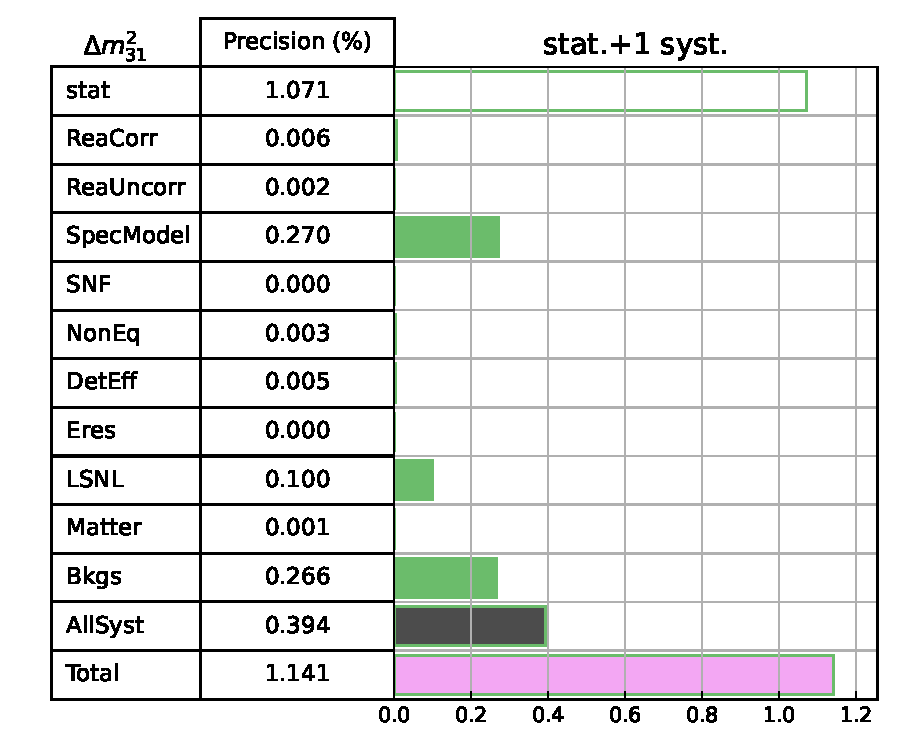
\includegraphics[width=\linewidth]{5_oscillation/dmsq31_50ds_juno_only.pdf}
%     \caption{50 days}
%     \label{fig:l1}
%   \end{subfigure}
%   \hfill
%   \begin{subfigure}[t]{0.32\textwidth}
%     \centering
%     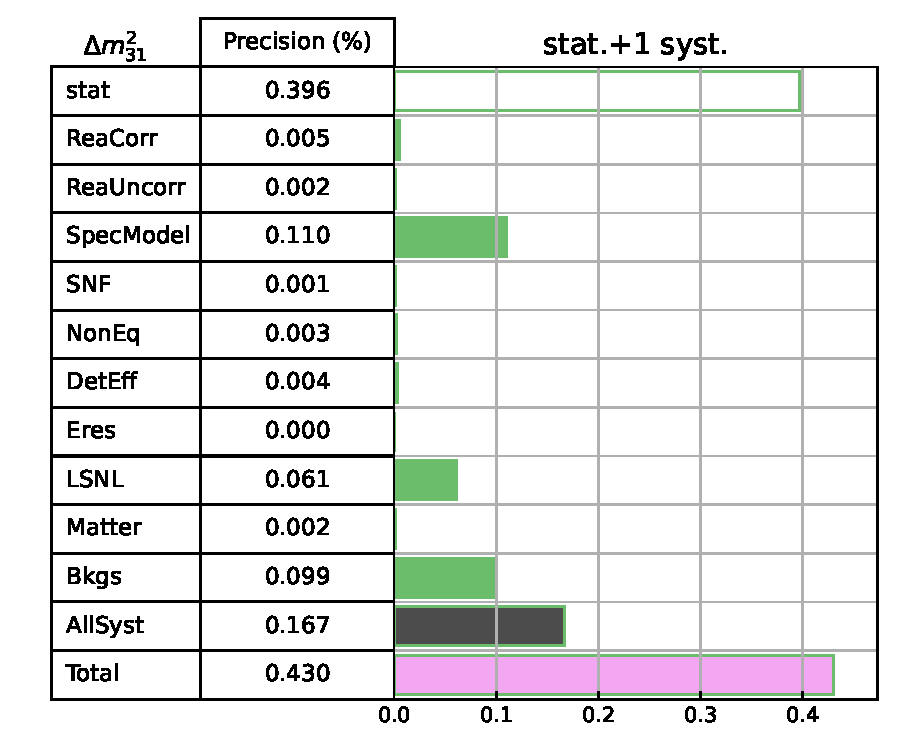
\includegraphics[width=\linewidth]{5_oscillation/dmsq31_1yr_juno_only.pdf}
%     \caption{1 year}
%     \label{fig:l2}
%   \end{subfigure}
%   \hfill
%   \begin{subfigure}[t]{0.32\textwidth}
%     \centering
%     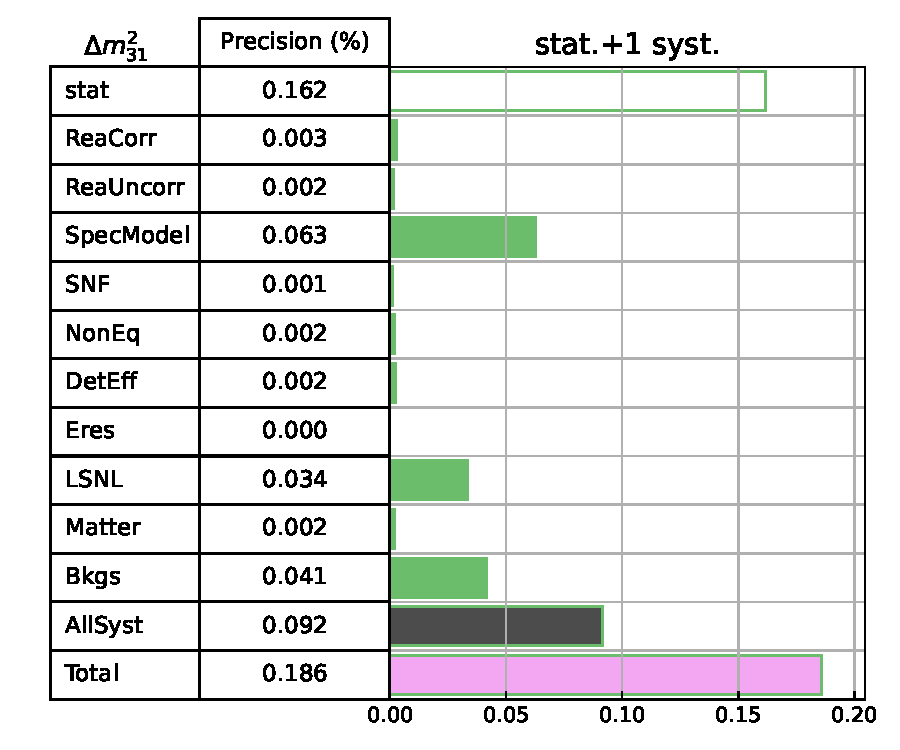
\includegraphics[width=\linewidth]{5_oscillation/dmsq31_6yr_juno_only.pdf}
%     \caption{6 years}
%     \label{fig:l3}
%   \end{subfigure}
%   \caption{Precision breakdown of $\rm \Delta m^2_{31}$}
%   %\label{Precision breakdown of $\rm \Delta m^2_{31}$}
% \end{figure}

\newpage

\bibliography{ref}

\end{document}
